\documentclass[twoside]{book}

% Packages required by doxygen
\usepackage{fixltx2e}
\usepackage{calc}
\usepackage{doxygen}
\usepackage[export]{adjustbox} % also loads graphicx
\usepackage{graphicx}
\usepackage[utf8]{inputenc}
\usepackage{makeidx}
\usepackage{multicol}
\usepackage{multirow}
\PassOptionsToPackage{warn}{textcomp}
\usepackage{textcomp}
\usepackage[nointegrals]{wasysym}
\usepackage[table]{xcolor}

% NLS support packages
\usepackage{hfont}

% Font selection
\usepackage[T1]{fontenc}
\usepackage[scaled=.90]{helvet}
\usepackage{courier}
\usepackage{amssymb}
\usepackage{sectsty}
\renewcommand{\familydefault}{\sfdefault}
\allsectionsfont{%
  \fontseries{bc}\selectfont%
  \color{darkgray}%
}
\renewcommand{\DoxyLabelFont}{%
  \fontseries{bc}\selectfont%
  \color{darkgray}%
}
\newcommand{\+}{\discretionary{\mbox{\scriptsize$\hookleftarrow$}}{}{}}

% Page & text layout
\usepackage{geometry}
\geometry{%
  a4paper,%
  top=2.5cm,%
  bottom=2.5cm,%
  left=2.5cm,%
  right=2.5cm%
}
\tolerance=750
\hfuzz=15pt
\hbadness=750
\setlength{\emergencystretch}{15pt}
\setlength{\parindent}{0cm}
\setlength{\parskip}{3ex plus 2ex minus 2ex}
\makeatletter
\renewcommand{\paragraph}{%
  \@startsection{paragraph}{4}{0ex}{-1.0ex}{1.0ex}{%
    \normalfont\normalsize\bfseries\SS@parafont%
  }%
}
\renewcommand{\subparagraph}{%
  \@startsection{subparagraph}{5}{0ex}{-1.0ex}{1.0ex}{%
    \normalfont\normalsize\bfseries\SS@subparafont%
  }%
}
\makeatother

% Headers & footers
\usepackage{fancyhdr}
\pagestyle{fancyplain}
\fancyhead[LE]{\fancyplain{}{\bfseries\thepage}}
\fancyhead[CE]{\fancyplain{}{}}
\fancyhead[RE]{\fancyplain{}{\bfseries\leftmark}}
\fancyhead[LO]{\fancyplain{}{\bfseries\rightmark}}
\fancyhead[CO]{\fancyplain{}{}}
\fancyhead[RO]{\fancyplain{}{\bfseries\thepage}}
\fancyfoot[LE]{\fancyplain{}{}}
\fancyfoot[CE]{\fancyplain{}{}}
\fancyfoot[RE]{\fancyplain{}{\bfseries\scriptsize 다음에 의해 생성됨 \+:  Doxygen }}
\fancyfoot[LO]{\fancyplain{}{\bfseries\scriptsize 다음에 의해 생성됨 \+:  Doxygen }}
\fancyfoot[CO]{\fancyplain{}{}}
\fancyfoot[RO]{\fancyplain{}{}}
\renewcommand{\footrulewidth}{0.4pt}
\renewcommand{\chaptermark}[1]{%
  \markboth{#1}{}%
}
\renewcommand{\sectionmark}[1]{%
  \markright{\thesection\ #1}%
}

% Indices & bibliography
\usepackage{natbib}
\usepackage[titles]{tocloft}
\setcounter{tocdepth}{3}
\setcounter{secnumdepth}{5}
\makeindex

% Hyperlinks (required, but should be loaded last)
\usepackage{ifpdf}
\ifpdf
  \usepackage[pdftex,pagebackref=true]{hyperref}
\else
  \usepackage[ps2pdf,pagebackref=true]{hyperref}
\fi
\hypersetup{%
  colorlinks=true,%
  linkcolor=blue,%
  citecolor=blue,%
  unicode%
}

% Custom commands
\newcommand{\clearemptydoublepage}{%
  \newpage{\pagestyle{empty}\cleardoublepage}%
}

\usepackage{caption}
\captionsetup{labelsep=space,justification=centering,font={bf},singlelinecheck=off,skip=4pt,position=top}

%===== C O N T E N T S =====

\begin{document}

% Titlepage & ToC
\hypersetup{pageanchor=false,
             bookmarksnumbered=true,
             pdfencoding=unicode
            }
\pagenumbering{alph}
\begin{titlepage}
\vspace*{7cm}
\begin{center}%
{\Large C\+U\+I\+\_\+\+Tetris \\[1ex]\large 1.\+0.\+0 }\\
\vspace*{1cm}
{\large 다음에 의해 생성됨 \+:  Doxygen 1.8.14}\\
\end{center}
\end{titlepage}
\clearemptydoublepage
\pagenumbering{roman}
\tableofcontents
\clearemptydoublepage
\pagenumbering{arabic}
\hypersetup{pageanchor=true}

%--- Begin generated contents ---
\chapter{계통도 색인}
\section{클래스 계통도}
이 상속 목록은 완전하진 않지만 알파벳순으로 대략적으로 정렬되어있습니다.\+:\begin{DoxyCompactList}
\item \contentsline{section}{Block}{\pageref{class_block}}{}
\begin{DoxyCompactList}
\item \contentsline{section}{I}{\pageref{class_i}}{}
\item \contentsline{section}{J}{\pageref{class_j}}{}
\item \contentsline{section}{L}{\pageref{class_l}}{}
\item \contentsline{section}{O}{\pageref{class_o}}{}
\item \contentsline{section}{S}{\pageref{class_s}}{}
\item \contentsline{section}{T}{\pageref{class_t}}{}
\item \contentsline{section}{Z}{\pageref{class_z}}{}
\end{DoxyCompactList}
\item \contentsline{section}{Block\+Handler}{\pageref{class_block_handler}}{}
\item \contentsline{section}{Board}{\pageref{class_board}}{}
\item \contentsline{section}{Board\+:\+:cell\+Info}{\pageref{struct_board_1_1cell_info}}{}
\item \contentsline{section}{Coord}{\pageref{struct_coord}}{}
\item \contentsline{section}{Drawer}{\pageref{class_drawer}}{}
\item \contentsline{section}{Game}{\pageref{class_game}}{}
\end{DoxyCompactList}

\chapter{클래스 색인}
\section{클래스 목록}
다음은 클래스, 구조체, 공용체 그리고 인터페이스들입니다. (간략한 설명만을 보여줍니다) \+:\begin{DoxyCompactList}
\item\contentsline{section}{\mbox{\hyperlink{class_block}{Block}} \\*모든 블럭의 Abstract Base Class }{\pageref{class_block}}{}
\item\contentsline{section}{\mbox{\hyperlink{class_block_handler}{Block\+Handler}} \\*Block을 생성하여 \mbox{\hyperlink{class_board}{Board}} 내에서 움직이도록 하는 클래스 }{\pageref{class_block_handler}}{}
\item\contentsline{section}{\mbox{\hyperlink{class_board}{Board}} \\*블럭이 배치될 보드 판 }{\pageref{class_board}}{}
\item\contentsline{section}{\mbox{\hyperlink{struct_board_1_1cell_info}{Board\+::cell\+Info}} \\*보드 내 각 셀에 대한 정보(채워져 있나 여부, 채운 블럭의 색상) 저장 }{\pageref{struct_board_1_1cell_info}}{}
\item\contentsline{section}{\mbox{\hyperlink{struct_coord}{Coord}} \\*\mbox{\hyperlink{class_board}{Board}} 내의 좌표와 \mbox{\hyperlink{class_block}{Block}} 모양의 좌표 형식 정보 표현 }{\pageref{struct_coord}}{}
\item\contentsline{section}{\mbox{\hyperlink{class_drawer}{Drawer}} \\*화면에 게임을 출력하는 클래스 }{\pageref{class_drawer}}{}
\item\contentsline{section}{\mbox{\hyperlink{class_game}{Game}} \\*\mbox{\hyperlink{class_board}{Board}}, \mbox{\hyperlink{class_block_handler}{Block\+Handler}}, Drawer를 이용하여 게임을 시작, 진행, 종료한다 }{\pageref{class_game}}{}
\item\contentsline{section}{\mbox{\hyperlink{class_i}{I}} \\*\mbox{\hyperlink{class_i}{I}} 모양 블럭 }{\pageref{class_i}}{}
\item\contentsline{section}{\mbox{\hyperlink{class_j}{J}} \\*\mbox{\hyperlink{class_j}{J}} 모양 블럭 }{\pageref{class_j}}{}
\item\contentsline{section}{\mbox{\hyperlink{class_l}{L}} \\*\mbox{\hyperlink{class_l}{L}} 모양 블럭 }{\pageref{class_l}}{}
\item\contentsline{section}{\mbox{\hyperlink{class_o}{O}} \\*ㅁ(네모) 모양 블럭 }{\pageref{class_o}}{}
\item\contentsline{section}{\mbox{\hyperlink{class_s}{S}} \\*\mbox{\hyperlink{class_s}{S}} 모양 블럭 }{\pageref{class_s}}{}
\item\contentsline{section}{\mbox{\hyperlink{class_t}{T}} \\*\mbox{\hyperlink{class_t}{T}} 모양 블럭 }{\pageref{class_t}}{}
\item\contentsline{section}{\mbox{\hyperlink{class_z}{Z}} \\*\mbox{\hyperlink{class_z}{Z}} 모양 블럭 }{\pageref{class_z}}{}
\end{DoxyCompactList}

\chapter{파일 색인}
\section{파일 목록}
다음은 모든 파일에 대한 목록입니다. (간략한 설명만을 보여줍니다) \+:\begin{DoxyCompactList}
\item\contentsline{section}{\mbox{\hyperlink{main_8cpp}{main.\+cpp}} }{\pageref{main_8cpp}}{}
\item\contentsline{section}{\mbox{\hyperlink{tetris__block_8h}{tetris\+\_\+block.\+h}} }{\pageref{tetris__block_8h}}{}
\item\contentsline{section}{\mbox{\hyperlink{tetris__blockhandler_8h}{tetris\+\_\+blockhandler.\+h}} }{\pageref{tetris__blockhandler_8h}}{}
\item\contentsline{section}{\mbox{\hyperlink{tetris__board_8h}{tetris\+\_\+board.\+h}} }{\pageref{tetris__board_8h}}{}
\item\contentsline{section}{\mbox{\hyperlink{tetris__drawer_8h}{tetris\+\_\+drawer.\+h}} }{\pageref{tetris__drawer_8h}}{}
\item\contentsline{section}{\mbox{\hyperlink{tetris__game_8h}{tetris\+\_\+game.\+h}} }{\pageref{tetris__game_8h}}{}
\end{DoxyCompactList}

\chapter{클래스 문서화}
\hypertarget{class_block}{}\section{Block 클래스 참조}
\label{class_block}\index{Block@{Block}}


모든 블럭의 Abstract Base Class.  




{\ttfamily \#include $<$tetris\+\_\+block.\+h$>$}



Block에 대한 상속 다이어그램 \+: 
\nopagebreak
\begin{figure}[H]
\begin{center}
\leavevmode
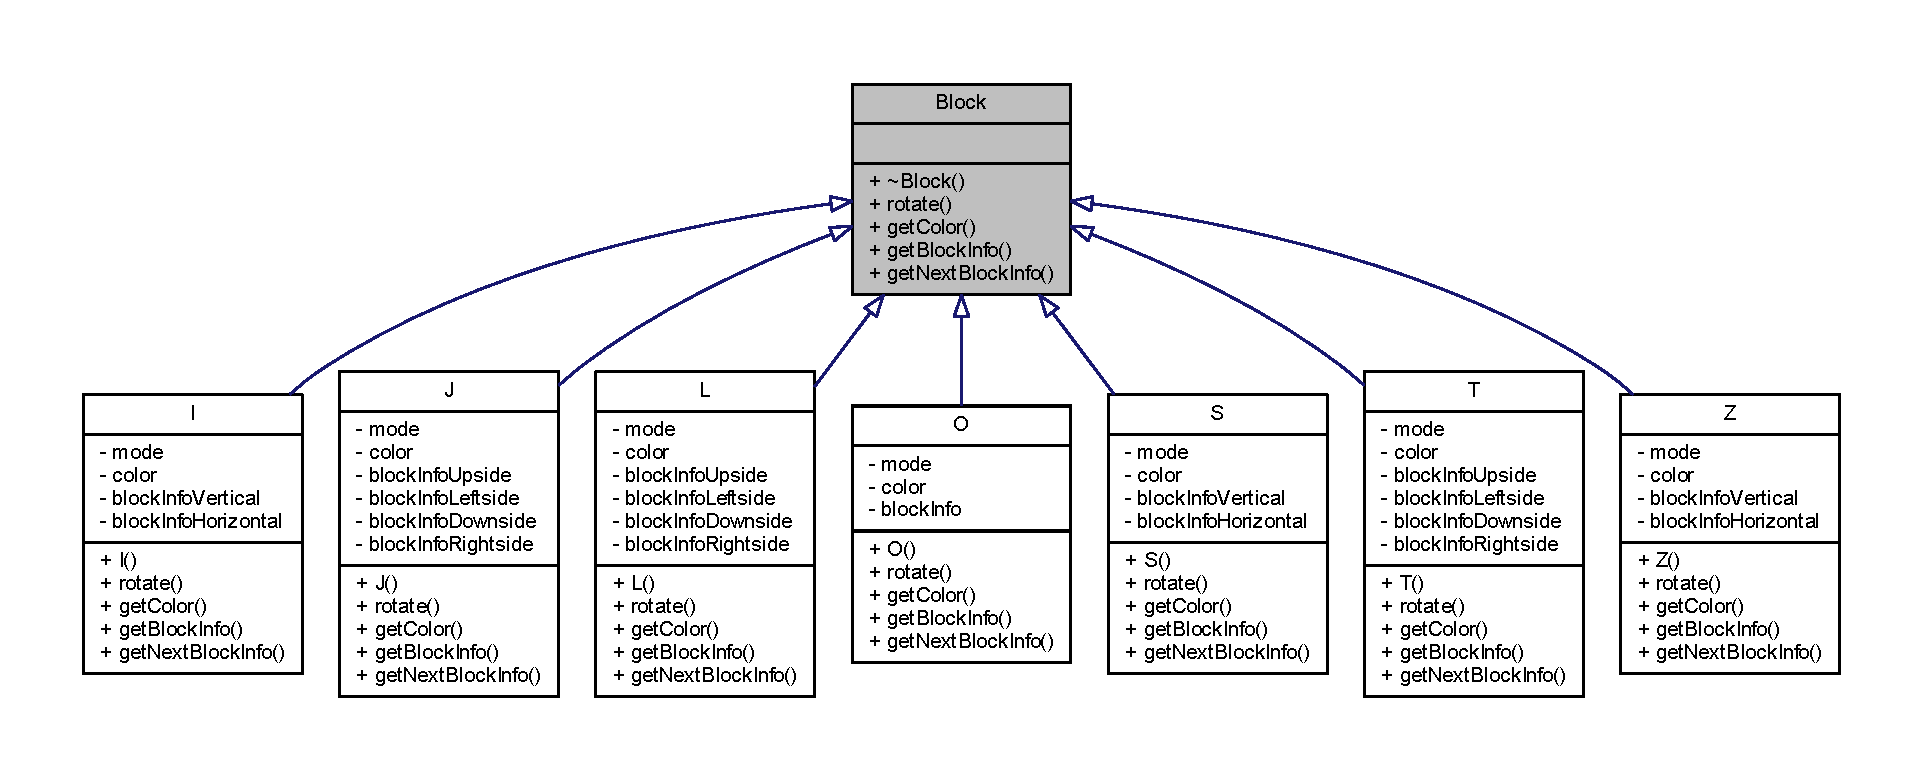
\includegraphics[width=350pt]{class_block__inherit__graph}
\end{center}
\end{figure}


Block에 대한 협력 다이어그램\+:
\nopagebreak
\begin{figure}[H]
\begin{center}
\leavevmode
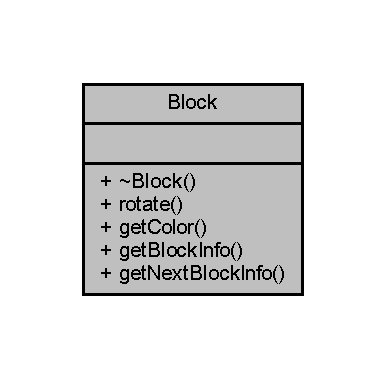
\includegraphics[width=185pt]{class_block__coll__graph}
\end{center}
\end{figure}
\subsection*{Public 타입}
\begin{DoxyCompactItemize}
\item 
enum \mbox{\hyperlink{class_block_a33a96023993478ad4b52426188454765}{Mode}} \{ \newline
\mbox{\hyperlink{class_block_a33a96023993478ad4b52426188454765a4529e89ca1c08cc5f81181e355719fad}{U\+P\+S\+I\+DE}}, 
\mbox{\hyperlink{class_block_a33a96023993478ad4b52426188454765a9c855bf91465e7da98901d7900740919}{L\+E\+F\+T\+S\+I\+DE}}, 
\mbox{\hyperlink{class_block_a33a96023993478ad4b52426188454765a73fd4ad0ff8642235ec8549f9290d13b}{D\+O\+W\+N\+S\+I\+DE}}, 
\mbox{\hyperlink{class_block_a33a96023993478ad4b52426188454765a005424e665ea0b83edfaf9ddb3ab85a1}{R\+I\+G\+H\+T\+S\+I\+DE}}, 
\newline
\mbox{\hyperlink{class_block_a33a96023993478ad4b52426188454765a76628d7877667ccb2f6e549b89466a4a}{V\+E\+R\+T\+I\+C\+AL}}, 
\mbox{\hyperlink{class_block_a33a96023993478ad4b52426188454765a883bda1b4a0cb6d25d8b3c3465f0cfef}{H\+O\+R\+I\+Z\+O\+N\+T\+AL}}
 \}
\begin{DoxyCompactList}\small\item\em 블럭들의 회전 상태를 나타내는 enum type \end{DoxyCompactList}\item 
enum \mbox{\hyperlink{class_block_ad054b4ac51df79aa910040b2a2fdf7b5}{Color}} \{ \newline
\mbox{\hyperlink{class_block_ad054b4ac51df79aa910040b2a2fdf7b5acd0cdefe1b7ef4fc0c9b47a765ae00ca}{B\+L\+A\+CK}}, 
\mbox{\hyperlink{class_block_ad054b4ac51df79aa910040b2a2fdf7b5a770f3d9456df6e3e286c001f0ffc835f}{B\+L\+UE}}, 
\mbox{\hyperlink{class_block_ad054b4ac51df79aa910040b2a2fdf7b5ac7f4e27e7581d2456d7db6b52514800d}{G\+R\+E\+EN}}, 
\mbox{\hyperlink{class_block_ad054b4ac51df79aa910040b2a2fdf7b5aa6acf45f9e85e879c50413b30769006a}{T\+U\+RQ}}, 
\newline
\mbox{\hyperlink{class_block_ad054b4ac51df79aa910040b2a2fdf7b5ac3d067e89682bb3d91db42beb7c68062}{R\+ED}}, 
\mbox{\hyperlink{class_block_ad054b4ac51df79aa910040b2a2fdf7b5adf5ec5d70a53f3465e863f43e9118588}{P\+U\+R\+P\+LE}}, 
\mbox{\hyperlink{class_block_ad054b4ac51df79aa910040b2a2fdf7b5a7ae21b7c7ed4cd37d641a5119d0b3939}{Y\+E\+L\+L\+OW}}, 
\mbox{\hyperlink{class_block_ad054b4ac51df79aa910040b2a2fdf7b5a37ab7320f3ca5662b117fb110adb1011}{W\+H\+I\+TE}}, 
\newline
\mbox{\hyperlink{class_block_ad054b4ac51df79aa910040b2a2fdf7b5a1158efe2e537f0b96f9ea590f22ab821}{G\+R\+AY}}, 
\mbox{\hyperlink{class_block_ad054b4ac51df79aa910040b2a2fdf7b5aad861330fd0e7f87dbfbe9ceb49785b3}{P\+A\+L\+E\+B\+L\+UE}}, 
\mbox{\hyperlink{class_block_ad054b4ac51df79aa910040b2a2fdf7b5ad7542730815e74f4f9a9df7fec33d3b5}{P\+A\+L\+E\+G\+R\+E\+EN}}, 
\mbox{\hyperlink{class_block_ad054b4ac51df79aa910040b2a2fdf7b5acbe4a64f95830b01b5be63b91544d452}{P\+A\+L\+E\+T\+U\+RQ}}, 
\newline
\mbox{\hyperlink{class_block_ad054b4ac51df79aa910040b2a2fdf7b5a9a1a56423a8c5b1b51fb11d184ced4cd}{P\+A\+L\+E\+R\+ED}}, 
\mbox{\hyperlink{class_block_ad054b4ac51df79aa910040b2a2fdf7b5ae78300d2e1540cc8a58c4018a2b902a6}{P\+A\+L\+E\+P\+U\+R\+P\+LE}}, 
\mbox{\hyperlink{class_block_ad054b4ac51df79aa910040b2a2fdf7b5ac09cccdee282b3a0c1331e2892042bea}{P\+A\+L\+E\+Y\+E\+L\+L\+OW}}, 
\mbox{\hyperlink{class_block_ad054b4ac51df79aa910040b2a2fdf7b5af606ae67cebcef81e9ee80f1411d4247}{B\+R\+I\+G\+H\+T\+W\+H\+I\+TE}}
 \}
\begin{DoxyCompactList}\small\item\em 블럭들이 가질 수 있는 색상을 나타내는 enum type \end{DoxyCompactList}\item 
typedef std\+::array$<$ \mbox{\hyperlink{struct_coord}{Coord}}, 4 $>$ \mbox{\hyperlink{class_block_aca5d951639f113e2ebd7856209d6b9ab}{Block\+Shape}}
\begin{DoxyCompactList}\small\item\em 블럭의 모양 정보를 좌표의 배열로 나타냄. \end{DoxyCompactList}\end{DoxyCompactItemize}
\subsection*{Public 멤버 함수}
\begin{DoxyCompactItemize}
\item 
virtual \mbox{\hyperlink{class_block_a9f0026f5d2dafca3c101e70e4b34780f}{$\sim$\+Block}} ()
\begin{DoxyCompactList}\small\item\em 가상 파괴자 \end{DoxyCompactList}\item 
virtual void \mbox{\hyperlink{class_block_af1499ad7e48fb750581b471d0d5bb0e0}{rotate}} ()=0
\begin{DoxyCompactList}\small\item\em 회전 상태를 다음 회전 상태로 변경 (한 번에 90도 회전) \end{DoxyCompactList}\item 
virtual const \mbox{\hyperlink{class_block_ad054b4ac51df79aa910040b2a2fdf7b5}{Color}} \mbox{\hyperlink{class_block_af10efef648f21dc708e42e149cd6fbcf}{get\+Color}} ()=0
\begin{DoxyCompactList}\small\item\em 블럭의 색상 정보를 리턴 \end{DoxyCompactList}\item 
virtual const \mbox{\hyperlink{class_block_aca5d951639f113e2ebd7856209d6b9ab}{Block\+Shape}} \& \mbox{\hyperlink{class_block_a2cdc0af223d621add42ac6c37fede329}{get\+Block\+Info}} ()=0
\begin{DoxyCompactList}\small\item\em 블럭의 현재 회전 상태에 따른 모양 정보 리턴 \end{DoxyCompactList}\item 
virtual const \mbox{\hyperlink{class_block_aca5d951639f113e2ebd7856209d6b9ab}{Block\+Shape}} \& \mbox{\hyperlink{class_block_a654da164e0493be9de6f2f2334bc73e8}{get\+Next\+Block\+Info}} ()=0
\begin{DoxyCompactList}\small\item\em 회전을 1번 더 했을 경우의 모양 정보 리턴 \end{DoxyCompactList}\end{DoxyCompactItemize}


\subsection{상세한 설명}
모든 블럭의 Abstract Base Class. 

tetris\+\_\+block.\+h 파일의 24 번째 라인에서 정의되었습니다.



\subsection{멤버 타입정의 문서화}
\mbox{\Hypertarget{class_block_aca5d951639f113e2ebd7856209d6b9ab}\label{class_block_aca5d951639f113e2ebd7856209d6b9ab}} 
\index{Block@{Block}!Block\+Shape@{Block\+Shape}}
\index{Block\+Shape@{Block\+Shape}!Block@{Block}}
\subsubsection{\texorpdfstring{Block\+Shape}{BlockShape}}
{\footnotesize\ttfamily typedef std\+::array$<$\mbox{\hyperlink{struct_coord}{Coord}}, 4$>$ \mbox{\hyperlink{class_block_aca5d951639f113e2ebd7856209d6b9ab}{Block\+::\+Block\+Shape}}}



블럭의 모양 정보를 좌표의 배열로 나타냄. 



tetris\+\_\+block.\+h 파일의 36 번째 라인에서 정의되었습니다.



\subsection{멤버 열거형 문서화}
\mbox{\Hypertarget{class_block_ad054b4ac51df79aa910040b2a2fdf7b5}\label{class_block_ad054b4ac51df79aa910040b2a2fdf7b5}} 
\index{Block@{Block}!Color@{Color}}
\index{Color@{Color}!Block@{Block}}
\subsubsection{\texorpdfstring{Color}{Color}}
{\footnotesize\ttfamily enum \mbox{\hyperlink{class_block_ad054b4ac51df79aa910040b2a2fdf7b5}{Block\+::\+Color}}}



블럭들이 가질 수 있는 색상을 나타내는 enum type 

\begin{DoxyEnumFields}{열거형 멤버}
\raisebox{\heightof{T}}[0pt][0pt]{\index{B\+L\+A\+CK@{B\+L\+A\+CK}!Block@{Block}}\index{Block@{Block}!B\+L\+A\+CK@{B\+L\+A\+CK}}}\mbox{\Hypertarget{class_block_ad054b4ac51df79aa910040b2a2fdf7b5acd0cdefe1b7ef4fc0c9b47a765ae00ca}\label{class_block_ad054b4ac51df79aa910040b2a2fdf7b5acd0cdefe1b7ef4fc0c9b47a765ae00ca}} 
B\+L\+A\+CK&\\
\hline

\raisebox{\heightof{T}}[0pt][0pt]{\index{B\+L\+UE@{B\+L\+UE}!Block@{Block}}\index{Block@{Block}!B\+L\+UE@{B\+L\+UE}}}\mbox{\Hypertarget{class_block_ad054b4ac51df79aa910040b2a2fdf7b5a770f3d9456df6e3e286c001f0ffc835f}\label{class_block_ad054b4ac51df79aa910040b2a2fdf7b5a770f3d9456df6e3e286c001f0ffc835f}} 
B\+L\+UE&\\
\hline

\raisebox{\heightof{T}}[0pt][0pt]{\index{G\+R\+E\+EN@{G\+R\+E\+EN}!Block@{Block}}\index{Block@{Block}!G\+R\+E\+EN@{G\+R\+E\+EN}}}\mbox{\Hypertarget{class_block_ad054b4ac51df79aa910040b2a2fdf7b5ac7f4e27e7581d2456d7db6b52514800d}\label{class_block_ad054b4ac51df79aa910040b2a2fdf7b5ac7f4e27e7581d2456d7db6b52514800d}} 
G\+R\+E\+EN&\\
\hline

\raisebox{\heightof{T}}[0pt][0pt]{\index{T\+U\+RQ@{T\+U\+RQ}!Block@{Block}}\index{Block@{Block}!T\+U\+RQ@{T\+U\+RQ}}}\mbox{\Hypertarget{class_block_ad054b4ac51df79aa910040b2a2fdf7b5aa6acf45f9e85e879c50413b30769006a}\label{class_block_ad054b4ac51df79aa910040b2a2fdf7b5aa6acf45f9e85e879c50413b30769006a}} 
T\+U\+RQ&\\
\hline

\raisebox{\heightof{T}}[0pt][0pt]{\index{R\+ED@{R\+ED}!Block@{Block}}\index{Block@{Block}!R\+ED@{R\+ED}}}\mbox{\Hypertarget{class_block_ad054b4ac51df79aa910040b2a2fdf7b5ac3d067e89682bb3d91db42beb7c68062}\label{class_block_ad054b4ac51df79aa910040b2a2fdf7b5ac3d067e89682bb3d91db42beb7c68062}} 
R\+ED&\\
\hline

\raisebox{\heightof{T}}[0pt][0pt]{\index{P\+U\+R\+P\+LE@{P\+U\+R\+P\+LE}!Block@{Block}}\index{Block@{Block}!P\+U\+R\+P\+LE@{P\+U\+R\+P\+LE}}}\mbox{\Hypertarget{class_block_ad054b4ac51df79aa910040b2a2fdf7b5adf5ec5d70a53f3465e863f43e9118588}\label{class_block_ad054b4ac51df79aa910040b2a2fdf7b5adf5ec5d70a53f3465e863f43e9118588}} 
P\+U\+R\+P\+LE&\\
\hline

\raisebox{\heightof{T}}[0pt][0pt]{\index{Y\+E\+L\+L\+OW@{Y\+E\+L\+L\+OW}!Block@{Block}}\index{Block@{Block}!Y\+E\+L\+L\+OW@{Y\+E\+L\+L\+OW}}}\mbox{\Hypertarget{class_block_ad054b4ac51df79aa910040b2a2fdf7b5a7ae21b7c7ed4cd37d641a5119d0b3939}\label{class_block_ad054b4ac51df79aa910040b2a2fdf7b5a7ae21b7c7ed4cd37d641a5119d0b3939}} 
Y\+E\+L\+L\+OW&\\
\hline

\raisebox{\heightof{T}}[0pt][0pt]{\index{W\+H\+I\+TE@{W\+H\+I\+TE}!Block@{Block}}\index{Block@{Block}!W\+H\+I\+TE@{W\+H\+I\+TE}}}\mbox{\Hypertarget{class_block_ad054b4ac51df79aa910040b2a2fdf7b5a37ab7320f3ca5662b117fb110adb1011}\label{class_block_ad054b4ac51df79aa910040b2a2fdf7b5a37ab7320f3ca5662b117fb110adb1011}} 
W\+H\+I\+TE&\\
\hline

\raisebox{\heightof{T}}[0pt][0pt]{\index{G\+R\+AY@{G\+R\+AY}!Block@{Block}}\index{Block@{Block}!G\+R\+AY@{G\+R\+AY}}}\mbox{\Hypertarget{class_block_ad054b4ac51df79aa910040b2a2fdf7b5a1158efe2e537f0b96f9ea590f22ab821}\label{class_block_ad054b4ac51df79aa910040b2a2fdf7b5a1158efe2e537f0b96f9ea590f22ab821}} 
G\+R\+AY&\\
\hline

\raisebox{\heightof{T}}[0pt][0pt]{\index{P\+A\+L\+E\+B\+L\+UE@{P\+A\+L\+E\+B\+L\+UE}!Block@{Block}}\index{Block@{Block}!P\+A\+L\+E\+B\+L\+UE@{P\+A\+L\+E\+B\+L\+UE}}}\mbox{\Hypertarget{class_block_ad054b4ac51df79aa910040b2a2fdf7b5aad861330fd0e7f87dbfbe9ceb49785b3}\label{class_block_ad054b4ac51df79aa910040b2a2fdf7b5aad861330fd0e7f87dbfbe9ceb49785b3}} 
P\+A\+L\+E\+B\+L\+UE&\\
\hline

\raisebox{\heightof{T}}[0pt][0pt]{\index{P\+A\+L\+E\+G\+R\+E\+EN@{P\+A\+L\+E\+G\+R\+E\+EN}!Block@{Block}}\index{Block@{Block}!P\+A\+L\+E\+G\+R\+E\+EN@{P\+A\+L\+E\+G\+R\+E\+EN}}}\mbox{\Hypertarget{class_block_ad054b4ac51df79aa910040b2a2fdf7b5ad7542730815e74f4f9a9df7fec33d3b5}\label{class_block_ad054b4ac51df79aa910040b2a2fdf7b5ad7542730815e74f4f9a9df7fec33d3b5}} 
P\+A\+L\+E\+G\+R\+E\+EN&\\
\hline

\raisebox{\heightof{T}}[0pt][0pt]{\index{P\+A\+L\+E\+T\+U\+RQ@{P\+A\+L\+E\+T\+U\+RQ}!Block@{Block}}\index{Block@{Block}!P\+A\+L\+E\+T\+U\+RQ@{P\+A\+L\+E\+T\+U\+RQ}}}\mbox{\Hypertarget{class_block_ad054b4ac51df79aa910040b2a2fdf7b5acbe4a64f95830b01b5be63b91544d452}\label{class_block_ad054b4ac51df79aa910040b2a2fdf7b5acbe4a64f95830b01b5be63b91544d452}} 
P\+A\+L\+E\+T\+U\+RQ&\\
\hline

\raisebox{\heightof{T}}[0pt][0pt]{\index{P\+A\+L\+E\+R\+ED@{P\+A\+L\+E\+R\+ED}!Block@{Block}}\index{Block@{Block}!P\+A\+L\+E\+R\+ED@{P\+A\+L\+E\+R\+ED}}}\mbox{\Hypertarget{class_block_ad054b4ac51df79aa910040b2a2fdf7b5a9a1a56423a8c5b1b51fb11d184ced4cd}\label{class_block_ad054b4ac51df79aa910040b2a2fdf7b5a9a1a56423a8c5b1b51fb11d184ced4cd}} 
P\+A\+L\+E\+R\+ED&\\
\hline

\raisebox{\heightof{T}}[0pt][0pt]{\index{P\+A\+L\+E\+P\+U\+R\+P\+LE@{P\+A\+L\+E\+P\+U\+R\+P\+LE}!Block@{Block}}\index{Block@{Block}!P\+A\+L\+E\+P\+U\+R\+P\+LE@{P\+A\+L\+E\+P\+U\+R\+P\+LE}}}\mbox{\Hypertarget{class_block_ad054b4ac51df79aa910040b2a2fdf7b5ae78300d2e1540cc8a58c4018a2b902a6}\label{class_block_ad054b4ac51df79aa910040b2a2fdf7b5ae78300d2e1540cc8a58c4018a2b902a6}} 
P\+A\+L\+E\+P\+U\+R\+P\+LE&\\
\hline

\raisebox{\heightof{T}}[0pt][0pt]{\index{P\+A\+L\+E\+Y\+E\+L\+L\+OW@{P\+A\+L\+E\+Y\+E\+L\+L\+OW}!Block@{Block}}\index{Block@{Block}!P\+A\+L\+E\+Y\+E\+L\+L\+OW@{P\+A\+L\+E\+Y\+E\+L\+L\+OW}}}\mbox{\Hypertarget{class_block_ad054b4ac51df79aa910040b2a2fdf7b5ac09cccdee282b3a0c1331e2892042bea}\label{class_block_ad054b4ac51df79aa910040b2a2fdf7b5ac09cccdee282b3a0c1331e2892042bea}} 
P\+A\+L\+E\+Y\+E\+L\+L\+OW&\\
\hline

\raisebox{\heightof{T}}[0pt][0pt]{\index{B\+R\+I\+G\+H\+T\+W\+H\+I\+TE@{B\+R\+I\+G\+H\+T\+W\+H\+I\+TE}!Block@{Block}}\index{Block@{Block}!B\+R\+I\+G\+H\+T\+W\+H\+I\+TE@{B\+R\+I\+G\+H\+T\+W\+H\+I\+TE}}}\mbox{\Hypertarget{class_block_ad054b4ac51df79aa910040b2a2fdf7b5af606ae67cebcef81e9ee80f1411d4247}\label{class_block_ad054b4ac51df79aa910040b2a2fdf7b5af606ae67cebcef81e9ee80f1411d4247}} 
B\+R\+I\+G\+H\+T\+W\+H\+I\+TE&\\
\hline

\end{DoxyEnumFields}


tetris\+\_\+block.\+h 파일의 31 번째 라인에서 정의되었습니다.


\begin{DoxyCode}
32     \{
33         \mbox{\hyperlink{class_block_ad054b4ac51df79aa910040b2a2fdf7b5acd0cdefe1b7ef4fc0c9b47a765ae00ca}{BLACK}}, \mbox{\hyperlink{class_block_ad054b4ac51df79aa910040b2a2fdf7b5a770f3d9456df6e3e286c001f0ffc835f}{BLUE}}, \mbox{\hyperlink{class_block_ad054b4ac51df79aa910040b2a2fdf7b5ac7f4e27e7581d2456d7db6b52514800d}{GREEN}}, \mbox{\hyperlink{class_block_ad054b4ac51df79aa910040b2a2fdf7b5aa6acf45f9e85e879c50413b30769006a}{TURQ}}, \mbox{\hyperlink{class_block_ad054b4ac51df79aa910040b2a2fdf7b5ac3d067e89682bb3d91db42beb7c68062}{RED}}, \mbox{\hyperlink{class_block_ad054b4ac51df79aa910040b2a2fdf7b5adf5ec5d70a53f3465e863f43e9118588}{PURPLE}}, \mbox{\hyperlink{class_block_ad054b4ac51df79aa910040b2a2fdf7b5a7ae21b7c7ed4cd37d641a5119d0b3939}{YELLOW}}, 
      \mbox{\hyperlink{class_block_ad054b4ac51df79aa910040b2a2fdf7b5a37ab7320f3ca5662b117fb110adb1011}{WHITE}}, \mbox{\hyperlink{class_block_ad054b4ac51df79aa910040b2a2fdf7b5a1158efe2e537f0b96f9ea590f22ab821}{GRAY}},
34         \mbox{\hyperlink{class_block_ad054b4ac51df79aa910040b2a2fdf7b5aad861330fd0e7f87dbfbe9ceb49785b3}{PALEBLUE}}, \mbox{\hyperlink{class_block_ad054b4ac51df79aa910040b2a2fdf7b5ad7542730815e74f4f9a9df7fec33d3b5}{PALEGREEN}}, \mbox{\hyperlink{class_block_ad054b4ac51df79aa910040b2a2fdf7b5acbe4a64f95830b01b5be63b91544d452}{PALETURQ}}, \mbox{\hyperlink{class_block_ad054b4ac51df79aa910040b2a2fdf7b5a9a1a56423a8c5b1b51fb11d184ced4cd}{PALERED}}, 
      \mbox{\hyperlink{class_block_ad054b4ac51df79aa910040b2a2fdf7b5ae78300d2e1540cc8a58c4018a2b902a6}{PALEPURPLE}}, \mbox{\hyperlink{class_block_ad054b4ac51df79aa910040b2a2fdf7b5ac09cccdee282b3a0c1331e2892042bea}{PALEYELLOW}}, \mbox{\hyperlink{class_block_ad054b4ac51df79aa910040b2a2fdf7b5af606ae67cebcef81e9ee80f1411d4247}{BRIGHTWHITE}}
35     \};
\end{DoxyCode}
\mbox{\Hypertarget{class_block_a33a96023993478ad4b52426188454765}\label{class_block_a33a96023993478ad4b52426188454765}} 
\index{Block@{Block}!Mode@{Mode}}
\index{Mode@{Mode}!Block@{Block}}
\subsubsection{\texorpdfstring{Mode}{Mode}}
{\footnotesize\ttfamily enum \mbox{\hyperlink{class_block_a33a96023993478ad4b52426188454765}{Block\+::\+Mode}}}



블럭들의 회전 상태를 나타내는 enum type 

\begin{DoxyEnumFields}{열거형 멤버}
\raisebox{\heightof{T}}[0pt][0pt]{\index{U\+P\+S\+I\+DE@{U\+P\+S\+I\+DE}!Block@{Block}}\index{Block@{Block}!U\+P\+S\+I\+DE@{U\+P\+S\+I\+DE}}}\mbox{\Hypertarget{class_block_a33a96023993478ad4b52426188454765a4529e89ca1c08cc5f81181e355719fad}\label{class_block_a33a96023993478ad4b52426188454765a4529e89ca1c08cc5f81181e355719fad}} 
U\+P\+S\+I\+DE&\\
\hline

\raisebox{\heightof{T}}[0pt][0pt]{\index{L\+E\+F\+T\+S\+I\+DE@{L\+E\+F\+T\+S\+I\+DE}!Block@{Block}}\index{Block@{Block}!L\+E\+F\+T\+S\+I\+DE@{L\+E\+F\+T\+S\+I\+DE}}}\mbox{\Hypertarget{class_block_a33a96023993478ad4b52426188454765a9c855bf91465e7da98901d7900740919}\label{class_block_a33a96023993478ad4b52426188454765a9c855bf91465e7da98901d7900740919}} 
L\+E\+F\+T\+S\+I\+DE&\\
\hline

\raisebox{\heightof{T}}[0pt][0pt]{\index{D\+O\+W\+N\+S\+I\+DE@{D\+O\+W\+N\+S\+I\+DE}!Block@{Block}}\index{Block@{Block}!D\+O\+W\+N\+S\+I\+DE@{D\+O\+W\+N\+S\+I\+DE}}}\mbox{\Hypertarget{class_block_a33a96023993478ad4b52426188454765a73fd4ad0ff8642235ec8549f9290d13b}\label{class_block_a33a96023993478ad4b52426188454765a73fd4ad0ff8642235ec8549f9290d13b}} 
D\+O\+W\+N\+S\+I\+DE&\\
\hline

\raisebox{\heightof{T}}[0pt][0pt]{\index{R\+I\+G\+H\+T\+S\+I\+DE@{R\+I\+G\+H\+T\+S\+I\+DE}!Block@{Block}}\index{Block@{Block}!R\+I\+G\+H\+T\+S\+I\+DE@{R\+I\+G\+H\+T\+S\+I\+DE}}}\mbox{\Hypertarget{class_block_a33a96023993478ad4b52426188454765a005424e665ea0b83edfaf9ddb3ab85a1}\label{class_block_a33a96023993478ad4b52426188454765a005424e665ea0b83edfaf9ddb3ab85a1}} 
R\+I\+G\+H\+T\+S\+I\+DE&\\
\hline

\raisebox{\heightof{T}}[0pt][0pt]{\index{V\+E\+R\+T\+I\+C\+AL@{V\+E\+R\+T\+I\+C\+AL}!Block@{Block}}\index{Block@{Block}!V\+E\+R\+T\+I\+C\+AL@{V\+E\+R\+T\+I\+C\+AL}}}\mbox{\Hypertarget{class_block_a33a96023993478ad4b52426188454765a76628d7877667ccb2f6e549b89466a4a}\label{class_block_a33a96023993478ad4b52426188454765a76628d7877667ccb2f6e549b89466a4a}} 
V\+E\+R\+T\+I\+C\+AL&\\
\hline

\raisebox{\heightof{T}}[0pt][0pt]{\index{H\+O\+R\+I\+Z\+O\+N\+T\+AL@{H\+O\+R\+I\+Z\+O\+N\+T\+AL}!Block@{Block}}\index{Block@{Block}!H\+O\+R\+I\+Z\+O\+N\+T\+AL@{H\+O\+R\+I\+Z\+O\+N\+T\+AL}}}\mbox{\Hypertarget{class_block_a33a96023993478ad4b52426188454765a883bda1b4a0cb6d25d8b3c3465f0cfef}\label{class_block_a33a96023993478ad4b52426188454765a883bda1b4a0cb6d25d8b3c3465f0cfef}} 
H\+O\+R\+I\+Z\+O\+N\+T\+AL&\\
\hline

\end{DoxyEnumFields}


tetris\+\_\+block.\+h 파일의 28 번째 라인에서 정의되었습니다.


\begin{DoxyCode}
28 \{ \mbox{\hyperlink{class_block_a33a96023993478ad4b52426188454765a4529e89ca1c08cc5f81181e355719fad}{UPSIDE}}, \mbox{\hyperlink{class_block_a33a96023993478ad4b52426188454765a9c855bf91465e7da98901d7900740919}{LEFTSIDE}}, \mbox{\hyperlink{class_block_a33a96023993478ad4b52426188454765a73fd4ad0ff8642235ec8549f9290d13b}{DOWNSIDE}}, \mbox{\hyperlink{class_block_a33a96023993478ad4b52426188454765a005424e665ea0b83edfaf9ddb3ab85a1}{RIGHTSIDE}}, \mbox{\hyperlink{class_block_a33a96023993478ad4b52426188454765a76628d7877667ccb2f6e549b89466a4a}{VERTICAL}}, 
      \mbox{\hyperlink{class_block_a33a96023993478ad4b52426188454765a883bda1b4a0cb6d25d8b3c3465f0cfef}{HORIZONTAL}} \}; 
\end{DoxyCode}


\subsection{생성자 \& 소멸자 문서화}
\mbox{\Hypertarget{class_block_a9f0026f5d2dafca3c101e70e4b34780f}\label{class_block_a9f0026f5d2dafca3c101e70e4b34780f}} 
\index{Block@{Block}!````~Block@{$\sim$\+Block}}
\index{````~Block@{$\sim$\+Block}!Block@{Block}}
\subsubsection{\texorpdfstring{$\sim$\+Block()}{~Block()}}
{\footnotesize\ttfamily virtual Block\+::$\sim$\+Block (\begin{DoxyParamCaption}{ }\end{DoxyParamCaption})\hspace{0.3cm}{\ttfamily [inline]}, {\ttfamily [virtual]}}



가상 파괴자 



tetris\+\_\+block.\+h 파일의 38 번째 라인에서 정의되었습니다.



\subsection{멤버 함수 문서화}
\mbox{\Hypertarget{class_block_a2cdc0af223d621add42ac6c37fede329}\label{class_block_a2cdc0af223d621add42ac6c37fede329}} 
\index{Block@{Block}!get\+Block\+Info@{get\+Block\+Info}}
\index{get\+Block\+Info@{get\+Block\+Info}!Block@{Block}}
\subsubsection{\texorpdfstring{get\+Block\+Info()}{getBlockInfo()}}
{\footnotesize\ttfamily virtual const \mbox{\hyperlink{class_block_aca5d951639f113e2ebd7856209d6b9ab}{Block\+Shape}}\& Block\+::get\+Block\+Info (\begin{DoxyParamCaption}{ }\end{DoxyParamCaption})\hspace{0.3cm}{\ttfamily [pure virtual]}}



블럭의 현재 회전 상태에 따른 모양 정보 리턴 



\mbox{\hyperlink{class_z_a95cca7076b1d1744d099f2a7db67fbf1}{Z}}, \mbox{\hyperlink{class_s_aedd52f4a59ed94415945a54e0a1a477b}{S}}, \mbox{\hyperlink{class_o_a608161f6603f07da95a9d26ac7f0cacb}{O}}, \mbox{\hyperlink{class_t_a7c4343dcdc6e48c8413e2d582cdbcea9}{T}}, \mbox{\hyperlink{class_l_a15b15422c8c61bda876d5a7ca68e7347}{L}}, \mbox{\hyperlink{class_j_a2ef290578088ff6206767f6624748284}{J}}, \mbox{\hyperlink{class_i_a21f835547d478a560c6616d8ca81e966}{I}}에서 구현되었습니다.

\mbox{\Hypertarget{class_block_af10efef648f21dc708e42e149cd6fbcf}\label{class_block_af10efef648f21dc708e42e149cd6fbcf}} 
\index{Block@{Block}!get\+Color@{get\+Color}}
\index{get\+Color@{get\+Color}!Block@{Block}}
\subsubsection{\texorpdfstring{get\+Color()}{getColor()}}
{\footnotesize\ttfamily virtual const \mbox{\hyperlink{class_block_ad054b4ac51df79aa910040b2a2fdf7b5}{Color}} Block\+::get\+Color (\begin{DoxyParamCaption}{ }\end{DoxyParamCaption})\hspace{0.3cm}{\ttfamily [pure virtual]}}



블럭의 색상 정보를 리턴 



\mbox{\hyperlink{class_z_a75f1e882dd5fb52b23bbd691da1e306e}{Z}}, \mbox{\hyperlink{class_s_a6b0a59fa5ae754544d2ad1c250f8dece}{S}}, \mbox{\hyperlink{class_o_a2ffa14a52f6fa0f6964f25f75e2909ad}{O}}, \mbox{\hyperlink{class_t_a1aebf9e5cf8cf319810b09cc5c619157}{T}}, \mbox{\hyperlink{class_l_a059120e541b527394d832e5994659652}{L}}, \mbox{\hyperlink{class_j_a9055b5b54907c2fe1b9973cd74fc9c3e}{J}}, \mbox{\hyperlink{class_i_afa15b62959b0207778d0db1763aff784}{I}}에서 구현되었습니다.

\mbox{\Hypertarget{class_block_a654da164e0493be9de6f2f2334bc73e8}\label{class_block_a654da164e0493be9de6f2f2334bc73e8}} 
\index{Block@{Block}!get\+Next\+Block\+Info@{get\+Next\+Block\+Info}}
\index{get\+Next\+Block\+Info@{get\+Next\+Block\+Info}!Block@{Block}}
\subsubsection{\texorpdfstring{get\+Next\+Block\+Info()}{getNextBlockInfo()}}
{\footnotesize\ttfamily virtual const \mbox{\hyperlink{class_block_aca5d951639f113e2ebd7856209d6b9ab}{Block\+Shape}}\& Block\+::get\+Next\+Block\+Info (\begin{DoxyParamCaption}{ }\end{DoxyParamCaption})\hspace{0.3cm}{\ttfamily [pure virtual]}}



회전을 1번 더 했을 경우의 모양 정보 리턴 



\mbox{\hyperlink{class_z_a6891b8f72f62e7bb3a606b0d8fc96c38}{Z}}, \mbox{\hyperlink{class_s_a48ef6d5f37afe48b14ea11fe00537c5e}{S}}, \mbox{\hyperlink{class_o_a76a288c5f887c3b24cc6cb1c03bcd9b1}{O}}, \mbox{\hyperlink{class_t_a70e028be061a3f56032317cbedccb2d3}{T}}, \mbox{\hyperlink{class_l_ae7744f0eb73bfc7bd92e1e6fcee6ec52}{L}}, \mbox{\hyperlink{class_j_aeeaf9ab45ccf61d0e7435e3d1bf04300}{J}}, \mbox{\hyperlink{class_i_ae5a6c09baa0575ff54446278a32a900a}{I}}에서 구현되었습니다.

\mbox{\Hypertarget{class_block_af1499ad7e48fb750581b471d0d5bb0e0}\label{class_block_af1499ad7e48fb750581b471d0d5bb0e0}} 
\index{Block@{Block}!rotate@{rotate}}
\index{rotate@{rotate}!Block@{Block}}
\subsubsection{\texorpdfstring{rotate()}{rotate()}}
{\footnotesize\ttfamily virtual void Block\+::rotate (\begin{DoxyParamCaption}{ }\end{DoxyParamCaption})\hspace{0.3cm}{\ttfamily [pure virtual]}}



회전 상태를 다음 회전 상태로 변경 (한 번에 90도 회전) 



\mbox{\hyperlink{class_z_aa2d629f1ad269cf21fe06b1e83ed70fa}{Z}}, \mbox{\hyperlink{class_s_a9d968087a1d499416a0ce91cce3c8f9f}{S}}, \mbox{\hyperlink{class_o_ae1c0b5ef6d51aa94765531f555b47cd0}{O}}, \mbox{\hyperlink{class_t_a56d86fc6d32cda1c47176a8b85bb6599}{T}}, \mbox{\hyperlink{class_l_aff0b530ac47a401c6f285d9ded2f997b}{L}}, \mbox{\hyperlink{class_j_a79f9fdd2b9542a95d3d2f82381b1cb62}{J}}, \mbox{\hyperlink{class_i_a5ee89d0f1ddc27429dfd0c83edf86ad5}{I}}에서 구현되었습니다.



이 클래스에 대한 문서화 페이지는 다음의 파일로부터 생성되었습니다.\+:\begin{DoxyCompactItemize}
\item 
\mbox{\hyperlink{tetris__block_8h}{tetris\+\_\+block.\+h}}\end{DoxyCompactItemize}

\hypertarget{class_block_handler}{}\section{Block\+Handler 클래스 참조}
\label{class_block_handler}\index{Block\+Handler@{Block\+Handler}}


Block을 생성하여 \mbox{\hyperlink{class_board}{Board}} 내에서 움직이도록 하는 클래스  




{\ttfamily \#include $<$tetris\+\_\+blockhandler.\+h$>$}



Block\+Handler에 대한 협력 다이어그램\+:
\nopagebreak
\begin{figure}[H]
\begin{center}
\leavevmode
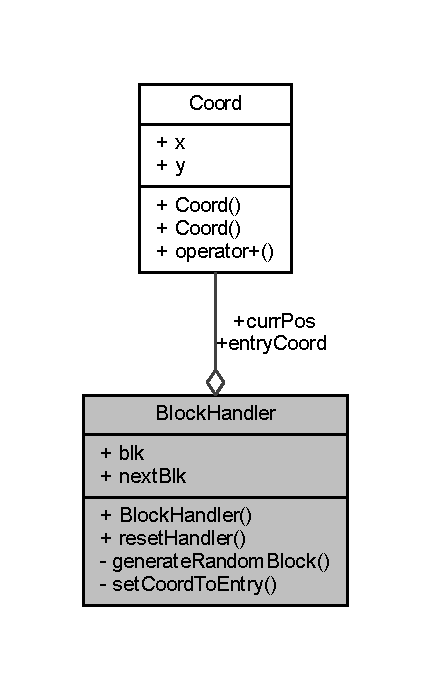
\includegraphics[width=207pt]{class_block_handler__coll__graph}
\end{center}
\end{figure}
\subsection*{Public 멤버 함수}
\begin{DoxyCompactItemize}
\item 
\mbox{\hyperlink{class_block_handler_ae1955a1830df4398795c153ef54804fa}{Block\+Handler}} (\mbox{\hyperlink{struct_coord}{Coord}} entry)
\begin{DoxyCompactList}\small\item\em 블럭 초기 설정 \end{DoxyCompactList}\item 
void \mbox{\hyperlink{class_block_handler_a170a8b83b6df72530675d722a17fb8c4}{reset\+Handler}} ()
\end{DoxyCompactItemize}
\subsection*{Public 속성}
\begin{DoxyCompactItemize}
\item 
\mbox{\hyperlink{struct_coord}{Coord}} \mbox{\hyperlink{class_block_handler_a11bd634fdc179446f9c6751e2394999e}{curr\+Pos}}
\begin{DoxyCompactList}\small\item\em Block의 \mbox{\hyperlink{class_board}{Board}} 내 현재 위치 \end{DoxyCompactList}\item 
std\+::unique\+\_\+ptr$<$ \mbox{\hyperlink{class_block}{Block}} $>$ \mbox{\hyperlink{class_block_handler_ab57212ded2552ab5559d278c8538c454}{blk}}
\begin{DoxyCompactList}\small\item\em 현재 블럭 \end{DoxyCompactList}\item 
std\+::unique\+\_\+ptr$<$ \mbox{\hyperlink{class_block}{Block}} $>$ \mbox{\hyperlink{class_block_handler_a7a7f96fa7c0d44f9e0fb5e52ebc9c428}{next\+Blk}}
\begin{DoxyCompactList}\small\item\em 다음에 배치될 블럭 \end{DoxyCompactList}\item 
\mbox{\hyperlink{struct_coord}{Coord}} \mbox{\hyperlink{class_block_handler_a5a2b1799763c46ced8a197775ca13fa7}{entry\+Coord}}
\begin{DoxyCompactList}\small\item\em \mbox{\hyperlink{class_board}{Board}} 내 초기 진입 위치 \end{DoxyCompactList}\end{DoxyCompactItemize}
\subsection*{Private 멤버 함수}
\begin{DoxyCompactItemize}
\item 
void \mbox{\hyperlink{class_block_handler_afaa88871c837a9af8fc407690aadffd6}{generate\+Random\+Block}} ()
\item 
void \mbox{\hyperlink{class_block_handler_aa0143a5722a52a91357c184354d484a6}{set\+Coord\+To\+Entry}} ()
\end{DoxyCompactItemize}


\subsection{상세한 설명}
Block을 생성하여 \mbox{\hyperlink{class_board}{Board}} 내에서 움직이도록 하는 클래스 

새 Block을 생성한다. 또한 그 다음에 배치될 Block에 대한 정보를 저장하고 있다. 그리고, 현재 Block의 \mbox{\hyperlink{class_board}{Board}} 내 위치와 진입 지점에 대한 정보를 가지고 있다. 

tetris\+\_\+blockhandler.\+h 파일의 14 번째 라인에서 정의되었습니다.



\subsection{생성자 \& 소멸자 문서화}
\mbox{\Hypertarget{class_block_handler_ae1955a1830df4398795c153ef54804fa}\label{class_block_handler_ae1955a1830df4398795c153ef54804fa}} 
\index{Block\+Handler@{Block\+Handler}!Block\+Handler@{Block\+Handler}}
\index{Block\+Handler@{Block\+Handler}!Block\+Handler@{Block\+Handler}}
\subsubsection{\texorpdfstring{Block\+Handler()}{BlockHandler()}}
{\footnotesize\ttfamily Block\+Handler\+::\+Block\+Handler (\begin{DoxyParamCaption}\item[{\mbox{\hyperlink{struct_coord}{Coord}}}]{entry }\end{DoxyParamCaption})\hspace{0.3cm}{\ttfamily [inline]}}



블럭 초기 설정 

\mbox{\hyperlink{class_board}{Board}} 내 초기 진입 위치를 저장하고, 현재 Block과 다음에 배치될 Block을 저장한다. 이후 현재 Block의 위치를 초기 위치로 설정한다. 
\begin{DoxyParams}{매개변수}
{\em \mbox{\hyperlink{struct_coord}{Coord}}} & entry \+: \mbox{\hyperlink{class_board}{Board}} 내 초기 진입 위치 \\
\hline
\end{DoxyParams}


tetris\+\_\+blockhandler.\+h 파일의 63 번째 라인에서 정의되었습니다.


\begin{DoxyCode}
64         : \mbox{\hyperlink{class_block_handler_ab57212ded2552ab5559d278c8538c454}{blk}}(\textcolor{keyword}{nullptr}), \mbox{\hyperlink{class_block_handler_a7a7f96fa7c0d44f9e0fb5e52ebc9c428}{nextBlk}}(\textcolor{keyword}{nullptr}), \mbox{\hyperlink{class_block_handler_a5a2b1799763c46ced8a197775ca13fa7}{entryCoord}}(entry), 
      \mbox{\hyperlink{class_block_handler_a11bd634fdc179446f9c6751e2394999e}{currPos}}(entry) 
65     \{
66         \mbox{\hyperlink{class_block_handler_afaa88871c837a9af8fc407690aadffd6}{generateRandomBlock}}();       \textcolor{comment}{// 현재 블럭을 위해 랜덤 블럭 생성}
67         \mbox{\hyperlink{class_block_handler_aa0143a5722a52a91357c184354d484a6}{setCoordToEntry}}();           \textcolor{comment}{// 현재 블럭의 초기 위치 설정}
68         \mbox{\hyperlink{class_block_handler_ab57212ded2552ab5559d278c8538c454}{blk}} = std::move(\mbox{\hyperlink{class_block_handler_a7a7f96fa7c0d44f9e0fb5e52ebc9c428}{nextBlk}}); \textcolor{comment}{// 생성한 랜덤 블럭을 현재 블럭에 인계}
69         \mbox{\hyperlink{class_block_handler_afaa88871c837a9af8fc407690aadffd6}{generateRandomBlock}}();       \textcolor{comment}{// 다음 블럭을 위한 블럭 생성}
70     \}
\end{DoxyCode}
이 함수 내부에서 호출하는 함수들에 대한 그래프입니다.\+:
\nopagebreak
\begin{figure}[H]
\begin{center}
\leavevmode
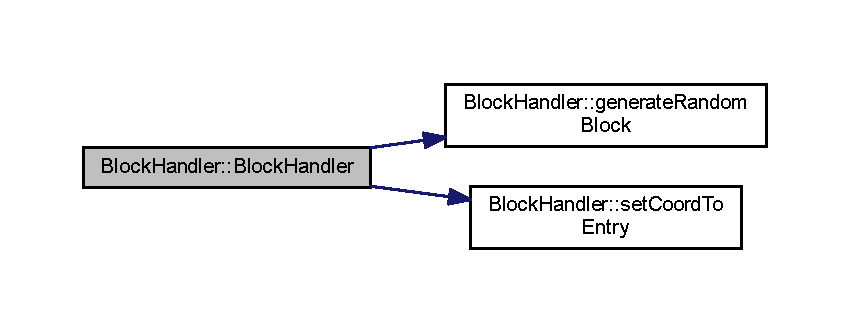
\includegraphics[width=350pt]{class_block_handler_ae1955a1830df4398795c153ef54804fa_cgraph}
\end{center}
\end{figure}


\subsection{멤버 함수 문서화}
\mbox{\Hypertarget{class_block_handler_afaa88871c837a9af8fc407690aadffd6}\label{class_block_handler_afaa88871c837a9af8fc407690aadffd6}} 
\index{Block\+Handler@{Block\+Handler}!generate\+Random\+Block@{generate\+Random\+Block}}
\index{generate\+Random\+Block@{generate\+Random\+Block}!Block\+Handler@{Block\+Handler}}
\subsubsection{\texorpdfstring{generate\+Random\+Block()}{generateRandomBlock()}}
{\footnotesize\ttfamily void Block\+Handler\+::generate\+Random\+Block (\begin{DoxyParamCaption}{ }\end{DoxyParamCaption})\hspace{0.3cm}{\ttfamily [inline]}, {\ttfamily [private]}}



tetris\+\_\+blockhandler.\+h 파일의 17 번째 라인에서 정의되었습니다.


\begin{DoxyCode}
18     \{
19         \textcolor{keywordflow}{switch} (std::rand() % 7)
20         \{
21         \textcolor{keywordflow}{case} 0:
22             \mbox{\hyperlink{class_block_handler_a7a7f96fa7c0d44f9e0fb5e52ebc9c428}{nextBlk}} = std::make\_unique<I>();
23             \textcolor{keywordflow}{break};
24         \textcolor{keywordflow}{case} 1:
25             \mbox{\hyperlink{class_block_handler_a7a7f96fa7c0d44f9e0fb5e52ebc9c428}{nextBlk}} = std::make\_unique<J>();
26             \textcolor{keywordflow}{break};
27         \textcolor{keywordflow}{case} 2:
28             \mbox{\hyperlink{class_block_handler_a7a7f96fa7c0d44f9e0fb5e52ebc9c428}{nextBlk}} = std::make\_unique<L>();
29             \textcolor{keywordflow}{break};
30         \textcolor{keywordflow}{case} 3:
31             \mbox{\hyperlink{class_block_handler_a7a7f96fa7c0d44f9e0fb5e52ebc9c428}{nextBlk}} = std::make\_unique<T>();
32             \textcolor{keywordflow}{break};
33         \textcolor{keywordflow}{case} 4:
34             \mbox{\hyperlink{class_block_handler_a7a7f96fa7c0d44f9e0fb5e52ebc9c428}{nextBlk}} = std::make\_unique<O>();
35             \textcolor{keywordflow}{break};
36         \textcolor{keywordflow}{case} 5:
37             \mbox{\hyperlink{class_block_handler_a7a7f96fa7c0d44f9e0fb5e52ebc9c428}{nextBlk}} = std::make\_unique<S>();
38             \textcolor{keywordflow}{break};
39         \textcolor{keywordflow}{case} 6:
40             \mbox{\hyperlink{class_block_handler_a7a7f96fa7c0d44f9e0fb5e52ebc9c428}{nextBlk}} = std::make\_unique<Z>();
41             \textcolor{keywordflow}{break};
42         \}
43     \}
\end{DoxyCode}
이 함수를 호출하는 함수들에 대한 그래프입니다.\+:
\nopagebreak
\begin{figure}[H]
\begin{center}
\leavevmode
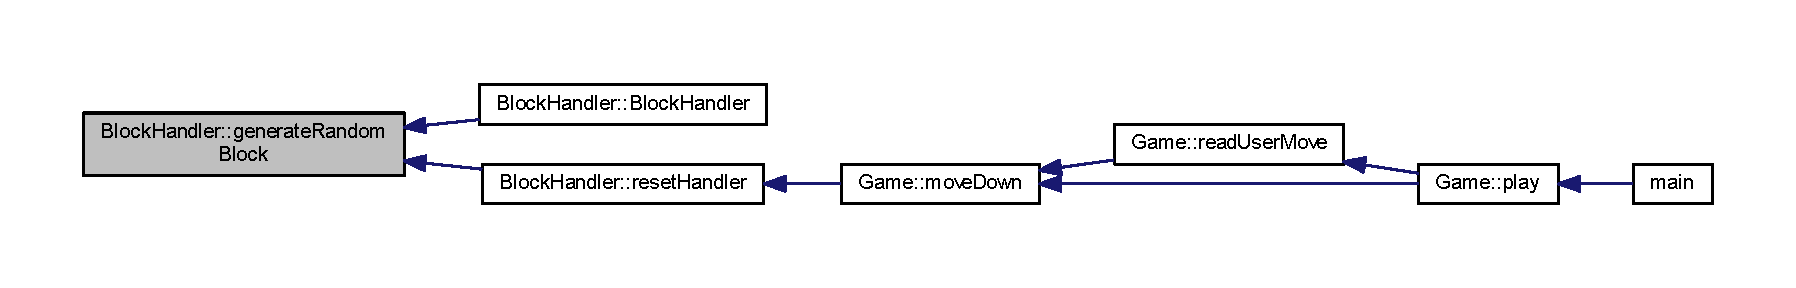
\includegraphics[width=350pt]{class_block_handler_afaa88871c837a9af8fc407690aadffd6_icgraph}
\end{center}
\end{figure}
\mbox{\Hypertarget{class_block_handler_a170a8b83b6df72530675d722a17fb8c4}\label{class_block_handler_a170a8b83b6df72530675d722a17fb8c4}} 
\index{Block\+Handler@{Block\+Handler}!reset\+Handler@{reset\+Handler}}
\index{reset\+Handler@{reset\+Handler}!Block\+Handler@{Block\+Handler}}
\subsubsection{\texorpdfstring{reset\+Handler()}{resetHandler()}}
{\footnotesize\ttfamily void Block\+Handler\+::reset\+Handler (\begin{DoxyParamCaption}{ }\end{DoxyParamCaption})\hspace{0.3cm}{\ttfamily [inline]}}



tetris\+\_\+blockhandler.\+h 파일의 72 번째 라인에서 정의되었습니다.


\begin{DoxyCode}
73     \{
74         \mbox{\hyperlink{class_block_handler_ab57212ded2552ab5559d278c8538c454}{blk}} = std::move(\mbox{\hyperlink{class_block_handler_a7a7f96fa7c0d44f9e0fb5e52ebc9c428}{nextBlk}}); 
75         \mbox{\hyperlink{class_block_handler_afaa88871c837a9af8fc407690aadffd6}{generateRandomBlock}}();
76         \mbox{\hyperlink{class_block_handler_aa0143a5722a52a91357c184354d484a6}{setCoordToEntry}}();
77     \}
\end{DoxyCode}
이 함수 내부에서 호출하는 함수들에 대한 그래프입니다.\+:
\nopagebreak
\begin{figure}[H]
\begin{center}
\leavevmode
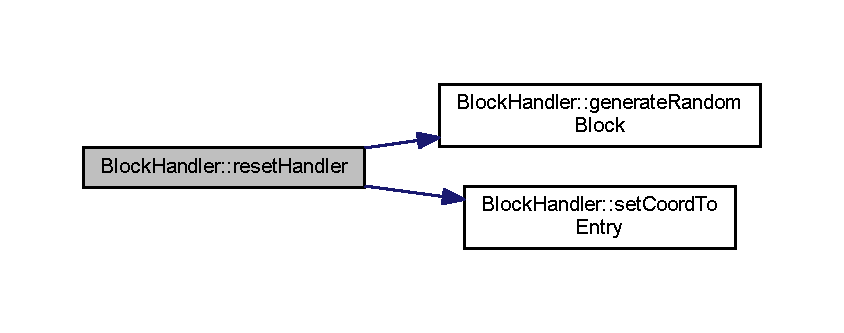
\includegraphics[width=350pt]{class_block_handler_a170a8b83b6df72530675d722a17fb8c4_cgraph}
\end{center}
\end{figure}
이 함수를 호출하는 함수들에 대한 그래프입니다.\+:
\nopagebreak
\begin{figure}[H]
\begin{center}
\leavevmode
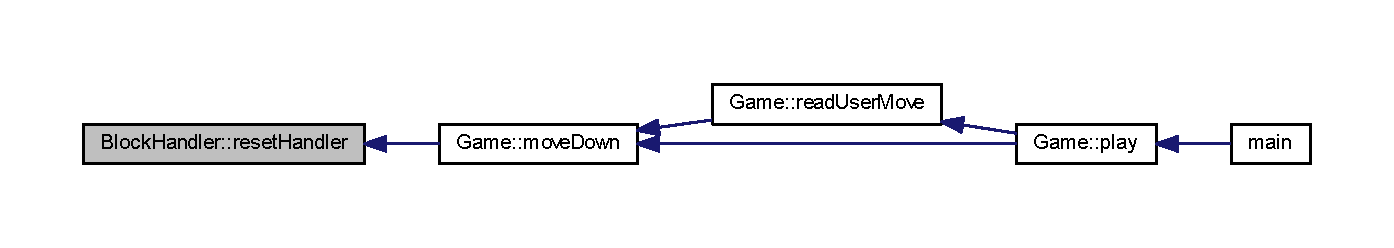
\includegraphics[width=350pt]{class_block_handler_a170a8b83b6df72530675d722a17fb8c4_icgraph}
\end{center}
\end{figure}
\mbox{\Hypertarget{class_block_handler_aa0143a5722a52a91357c184354d484a6}\label{class_block_handler_aa0143a5722a52a91357c184354d484a6}} 
\index{Block\+Handler@{Block\+Handler}!set\+Coord\+To\+Entry@{set\+Coord\+To\+Entry}}
\index{set\+Coord\+To\+Entry@{set\+Coord\+To\+Entry}!Block\+Handler@{Block\+Handler}}
\subsubsection{\texorpdfstring{set\+Coord\+To\+Entry()}{setCoordToEntry()}}
{\footnotesize\ttfamily void Block\+Handler\+::set\+Coord\+To\+Entry (\begin{DoxyParamCaption}{ }\end{DoxyParamCaption})\hspace{0.3cm}{\ttfamily [inline]}, {\ttfamily [private]}}



tetris\+\_\+blockhandler.\+h 파일의 45 번째 라인에서 정의되었습니다.


\begin{DoxyCode}
46     \{
47         \mbox{\hyperlink{class_block_handler_a11bd634fdc179446f9c6751e2394999e}{currPos}} = \mbox{\hyperlink{class_block_handler_a5a2b1799763c46ced8a197775ca13fa7}{entryCoord}};
48     \}
\end{DoxyCode}
이 함수를 호출하는 함수들에 대한 그래프입니다.\+:
\nopagebreak
\begin{figure}[H]
\begin{center}
\leavevmode
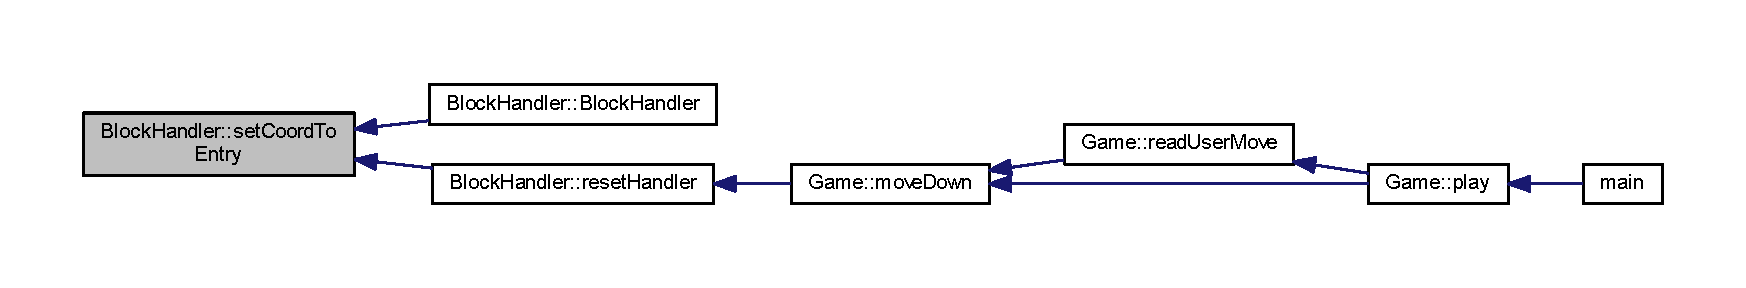
\includegraphics[width=350pt]{class_block_handler_aa0143a5722a52a91357c184354d484a6_icgraph}
\end{center}
\end{figure}


\subsection{멤버 데이터 문서화}
\mbox{\Hypertarget{class_block_handler_ab57212ded2552ab5559d278c8538c454}\label{class_block_handler_ab57212ded2552ab5559d278c8538c454}} 
\index{Block\+Handler@{Block\+Handler}!blk@{blk}}
\index{blk@{blk}!Block\+Handler@{Block\+Handler}}
\subsubsection{\texorpdfstring{blk}{blk}}
{\footnotesize\ttfamily std\+::unique\+\_\+ptr$<$\mbox{\hyperlink{class_block}{Block}}$>$ Block\+Handler\+::blk}



현재 블럭 



tetris\+\_\+blockhandler.\+h 파일의 52 번째 라인에서 정의되었습니다.

\mbox{\Hypertarget{class_block_handler_a11bd634fdc179446f9c6751e2394999e}\label{class_block_handler_a11bd634fdc179446f9c6751e2394999e}} 
\index{Block\+Handler@{Block\+Handler}!curr\+Pos@{curr\+Pos}}
\index{curr\+Pos@{curr\+Pos}!Block\+Handler@{Block\+Handler}}
\subsubsection{\texorpdfstring{curr\+Pos}{currPos}}
{\footnotesize\ttfamily \mbox{\hyperlink{struct_coord}{Coord}} Block\+Handler\+::curr\+Pos}



Block의 \mbox{\hyperlink{class_board}{Board}} 내 현재 위치 



tetris\+\_\+blockhandler.\+h 파일의 51 번째 라인에서 정의되었습니다.

\mbox{\Hypertarget{class_block_handler_a5a2b1799763c46ced8a197775ca13fa7}\label{class_block_handler_a5a2b1799763c46ced8a197775ca13fa7}} 
\index{Block\+Handler@{Block\+Handler}!entry\+Coord@{entry\+Coord}}
\index{entry\+Coord@{entry\+Coord}!Block\+Handler@{Block\+Handler}}
\subsubsection{\texorpdfstring{entry\+Coord}{entryCoord}}
{\footnotesize\ttfamily \mbox{\hyperlink{struct_coord}{Coord}} Block\+Handler\+::entry\+Coord}



\mbox{\hyperlink{class_board}{Board}} 내 초기 진입 위치 



tetris\+\_\+blockhandler.\+h 파일의 54 번째 라인에서 정의되었습니다.

\mbox{\Hypertarget{class_block_handler_a7a7f96fa7c0d44f9e0fb5e52ebc9c428}\label{class_block_handler_a7a7f96fa7c0d44f9e0fb5e52ebc9c428}} 
\index{Block\+Handler@{Block\+Handler}!next\+Blk@{next\+Blk}}
\index{next\+Blk@{next\+Blk}!Block\+Handler@{Block\+Handler}}
\subsubsection{\texorpdfstring{next\+Blk}{nextBlk}}
{\footnotesize\ttfamily std\+::unique\+\_\+ptr$<$\mbox{\hyperlink{class_block}{Block}}$>$ Block\+Handler\+::next\+Blk}



다음에 배치될 블럭 



tetris\+\_\+blockhandler.\+h 파일의 53 번째 라인에서 정의되었습니다.



이 클래스에 대한 문서화 페이지는 다음의 파일로부터 생성되었습니다.\+:\begin{DoxyCompactItemize}
\item 
\mbox{\hyperlink{tetris__blockhandler_8h}{tetris\+\_\+blockhandler.\+h}}\end{DoxyCompactItemize}

\hypertarget{class_board}{}\section{Board 클래스 참조}
\label{class_board}\index{Board@{Board}}


블럭이 배치될 보드 판.  




{\ttfamily \#include $<$tetris\+\_\+board.\+h$>$}



Board에 대한 협력 다이어그램\+:
\nopagebreak
\begin{figure}[H]
\begin{center}
\leavevmode
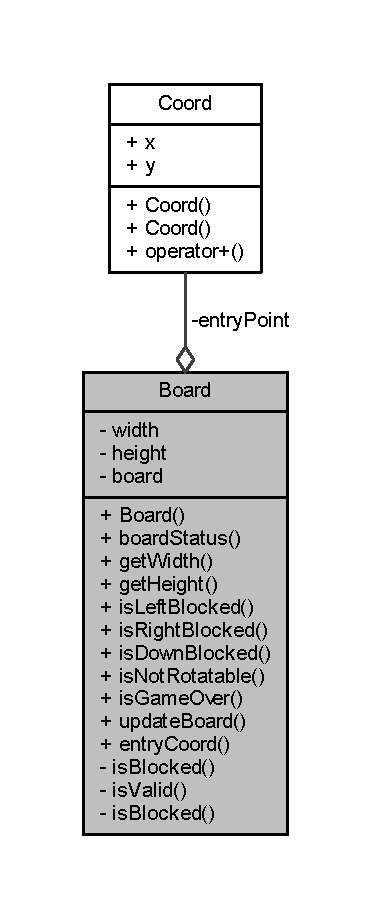
\includegraphics[width=180pt]{class_board__coll__graph}
\end{center}
\end{figure}
\subsection*{클래스}
\begin{DoxyCompactItemize}
\item 
struct \mbox{\hyperlink{struct_board_1_1cell_info}{cell\+Info}}
\begin{DoxyCompactList}\small\item\em 보드 내 각 셀에 대한 정보(채워져 있나 여부, 채운 블럭의 색상) 저장. \end{DoxyCompactList}\end{DoxyCompactItemize}
\subsection*{Public 타입}
\begin{DoxyCompactItemize}
\item 
typedef std\+::array$<$ std\+::array$<$ \mbox{\hyperlink{struct_board_1_1cell_info}{cell\+Info}}, 10 $>$, 25 $>$ \mbox{\hyperlink{class_board_a84bf794bc185e31e333b78bb003c4bc3}{Board\+Type}}
\begin{DoxyCompactList}\small\item\em 25 $\ast$ 10의 \mbox{\hyperlink{struct_board_1_1cell_info}{cell\+Info}} 2차원 배열로 보드를 나타냄 \end{DoxyCompactList}\end{DoxyCompactItemize}
\subsection*{Public 멤버 함수}
\begin{DoxyCompactItemize}
\item 
\mbox{\hyperlink{class_board_a9ee491d4fea680cf69b033374a9fdfcb}{Board}} ()
\begin{DoxyCompactList}\small\item\em 25 $\ast$ 10 보드를 생성하고, 진입 지점을 설정한다. \end{DoxyCompactList}\item 
const \mbox{\hyperlink{class_board_a84bf794bc185e31e333b78bb003c4bc3}{Board\+Type}} \& \mbox{\hyperlink{class_board_ac96b4da16e8dc266b39772f2da3fd7e2}{board\+Status}} () const
\begin{DoxyCompactList}\small\item\em 보드의 현재 상태를 리턴한다 \end{DoxyCompactList}\item 
int \mbox{\hyperlink{class_board_a31bdad2985e3b4857a383dd2da8e8e27}{get\+Width}} () const
\begin{DoxyCompactList}\small\item\em 보드의 너비를 리턴한다 \end{DoxyCompactList}\item 
int \mbox{\hyperlink{class_board_a888725ae3b1177a60a8f77299c1c939a}{get\+Height}} () const
\begin{DoxyCompactList}\small\item\em 보드의 높이를 리턴한다 \end{DoxyCompactList}\item 
bool \mbox{\hyperlink{class_board_a5545704e21b5f7447eb9ffe014954cb3}{is\+Left\+Blocked}} (const \mbox{\hyperlink{class_block_handler}{Block\+Handler}} \&handler) const
\begin{DoxyCompactList}\small\item\em 현재 블럭의 왼쪽이 막혀 있는 지를 리턴 \end{DoxyCompactList}\item 
bool \mbox{\hyperlink{class_board_ad38cdb8757f58a32b5747e2b7e0be277}{is\+Right\+Blocked}} (const \mbox{\hyperlink{class_block_handler}{Block\+Handler}} \&handler) const
\begin{DoxyCompactList}\small\item\em 현재 블럭의 오른쪽이 막혀 있는 지를 리턴 \end{DoxyCompactList}\item 
bool \mbox{\hyperlink{class_board_ad617ae22e46d1a62ed33592b20e00b44}{is\+Down\+Blocked}} (const \mbox{\hyperlink{class_block_handler}{Block\+Handler}} \&handler) const
\begin{DoxyCompactList}\small\item\em 현재 블럭의 아래가 막혀 있는 지를 리턴 \end{DoxyCompactList}\item 
bool \mbox{\hyperlink{class_board_a4b84310dd1ac3a08a3180361508a43e3}{is\+Not\+Rotatable}} (const \mbox{\hyperlink{class_block_handler}{Block\+Handler}} \&handler) const
\begin{DoxyCompactList}\small\item\em 현재 블럭이 회전 불가능한지를 리턴 \end{DoxyCompactList}\item 
bool \mbox{\hyperlink{class_board_a538ca2c02fbccf3af07ed3c821d9a736}{is\+Game\+Over}} (const \mbox{\hyperlink{class_block_handler}{Block\+Handler}} \&handler) const
\begin{DoxyCompactList}\small\item\em 현재 블럭이 보드에 진입 가능한지를 리턴 \end{DoxyCompactList}\item 
void \mbox{\hyperlink{class_board_a06e5188ef352fc5c0e3957895cef6a89}{update\+Board}} (const \mbox{\hyperlink{class_block_handler}{Block\+Handler}} \&handler)
\begin{DoxyCompactList}\small\item\em 블럭이 끝에 도달했을 때, 이를 보드에 기록한다. 줄이 꽉찼다면 보드를 새로 고친다. \end{DoxyCompactList}\item 
\mbox{\hyperlink{struct_coord}{Coord}} \mbox{\hyperlink{class_board_a902cd3b288be772ba6b7abc6a822afea}{entry\+Coord}} () const
\begin{DoxyCompactList}\small\item\em 진입 지점을 리턴한다 \end{DoxyCompactList}\end{DoxyCompactItemize}
\subsection*{Private 멤버 함수}
\begin{DoxyCompactItemize}
\item 
bool \mbox{\hyperlink{class_board_a61ff9b1284e5c3e1214a780361ed650b}{is\+Blocked}} (const \mbox{\hyperlink{struct_coord}{Coord}} \&dest) const
\begin{DoxyCompactList}\small\item\em 좌표에 해당하는 자리에 이미 블럭이 있는지를 리턴 \end{DoxyCompactList}\item 
bool \mbox{\hyperlink{class_board_a5df9c4c18c53b8029e0a080e5e089732}{is\+Valid}} (const \mbox{\hyperlink{struct_coord}{Coord}} \&dest) const
\item 
bool \mbox{\hyperlink{class_board_a1ba0d2a44e1469738220b5ff7dfda6fc}{is\+Blocked}} (const \mbox{\hyperlink{struct_coord}{Coord}} \&curr\+Pos, const \mbox{\hyperlink{class_block_aca5d951639f113e2ebd7856209d6b9ab}{Block\+::\+Block\+Shape}} \&block\+Shape) const
\begin{DoxyCompactList}\small\item\em 해당하는 자리가 막혀있는지를 리턴 \end{DoxyCompactList}\end{DoxyCompactItemize}
\subsection*{Private 속성}
\begin{DoxyCompactItemize}
\item 
const int \mbox{\hyperlink{class_board_a5c5b64d99e3c653c425206d2babf2f97}{width}}
\begin{DoxyCompactList}\small\item\em 보드의 너비(25) \end{DoxyCompactList}\item 
const int \mbox{\hyperlink{class_board_a37b65287f3b416ed31b0f15cfd9b3f7c}{height}}
\begin{DoxyCompactList}\small\item\em 보드의 높이(10) \end{DoxyCompactList}\item 
\mbox{\hyperlink{class_board_a84bf794bc185e31e333b78bb003c4bc3}{Board\+Type}} \mbox{\hyperlink{class_board_ad26aada4f19d2ca0c7bd534e8f466b6b}{board}} \{\}
\begin{DoxyCompactList}\small\item\em 보드(\mbox{\hyperlink{struct_board_1_1cell_info}{cell\+Info}} 2차원 배열) \end{DoxyCompactList}\item 
const \mbox{\hyperlink{struct_coord}{Coord}} \mbox{\hyperlink{class_board_a51d0b870dfe79367034bdda967e63a82}{entry\+Point}}
\begin{DoxyCompactList}\small\item\em 보드 내 블럭의 진입 지점 -\/ width와 height 다음에 선언되어야 한다 \end{DoxyCompactList}\end{DoxyCompactItemize}


\subsection{상세한 설명}
블럭이 배치될 보드 판. 

tetris\+\_\+board.\+h 파일의 12 번째 라인에서 정의되었습니다.



\subsection{멤버 타입정의 문서화}
\mbox{\Hypertarget{class_board_a84bf794bc185e31e333b78bb003c4bc3}\label{class_board_a84bf794bc185e31e333b78bb003c4bc3}} 
\index{Board@{Board}!Board\+Type@{Board\+Type}}
\index{Board\+Type@{Board\+Type}!Board@{Board}}
\subsubsection{\texorpdfstring{Board\+Type}{BoardType}}
{\footnotesize\ttfamily typedef std\+::array$<$std\+::array$<$\mbox{\hyperlink{struct_board_1_1cell_info}{cell\+Info}}, 10$>$, 25$>$ \mbox{\hyperlink{class_board_a84bf794bc185e31e333b78bb003c4bc3}{Board\+::\+Board\+Type}}}



25 $\ast$ 10의 \mbox{\hyperlink{struct_board_1_1cell_info}{cell\+Info}} 2차원 배열로 보드를 나타냄 



tetris\+\_\+board.\+h 파일의 24 번째 라인에서 정의되었습니다.



\subsection{생성자 \& 소멸자 문서화}
\mbox{\Hypertarget{class_board_a9ee491d4fea680cf69b033374a9fdfcb}\label{class_board_a9ee491d4fea680cf69b033374a9fdfcb}} 
\index{Board@{Board}!Board@{Board}}
\index{Board@{Board}!Board@{Board}}
\subsubsection{\texorpdfstring{Board()}{Board()}}
{\footnotesize\ttfamily Board\+::\+Board (\begin{DoxyParamCaption}{ }\end{DoxyParamCaption})\hspace{0.3cm}{\ttfamily [inline]}}



25 $\ast$ 10 보드를 생성하고, 진입 지점을 설정한다. 



tetris\+\_\+board.\+h 파일의 67 번째 라인에서 정의되었습니다.


\begin{DoxyCode}
67             : \mbox{\hyperlink{class_board_a5c5b64d99e3c653c425206d2babf2f97}{width}}(10), \mbox{\hyperlink{class_board_a37b65287f3b416ed31b0f15cfd9b3f7c}{height}}(25), \mbox{\hyperlink{class_board_a51d0b870dfe79367034bdda967e63a82}{entryPoint}}(\mbox{\hyperlink{class_board_a5c5b64d99e3c653c425206d2babf2f97}{width}} / 2, 1)
68     \{
69         
70     \}
\end{DoxyCode}


\subsection{멤버 함수 문서화}
\mbox{\Hypertarget{class_board_ac96b4da16e8dc266b39772f2da3fd7e2}\label{class_board_ac96b4da16e8dc266b39772f2da3fd7e2}} 
\index{Board@{Board}!board\+Status@{board\+Status}}
\index{board\+Status@{board\+Status}!Board@{Board}}
\subsubsection{\texorpdfstring{board\+Status()}{boardStatus()}}
{\footnotesize\ttfamily const \mbox{\hyperlink{class_board_a84bf794bc185e31e333b78bb003c4bc3}{Board\+Type}}\& Board\+::board\+Status (\begin{DoxyParamCaption}{ }\end{DoxyParamCaption}) const\hspace{0.3cm}{\ttfamily [inline]}}



보드의 현재 상태를 리턴한다 



tetris\+\_\+board.\+h 파일의 73 번째 라인에서 정의되었습니다.


\begin{DoxyCode}
74     \{
75         \textcolor{keywordflow}{return} \mbox{\hyperlink{class_board_ad26aada4f19d2ca0c7bd534e8f466b6b}{board}};
76     \}
\end{DoxyCode}
이 함수를 호출하는 함수들에 대한 그래프입니다.\+:
\nopagebreak
\begin{figure}[H]
\begin{center}
\leavevmode
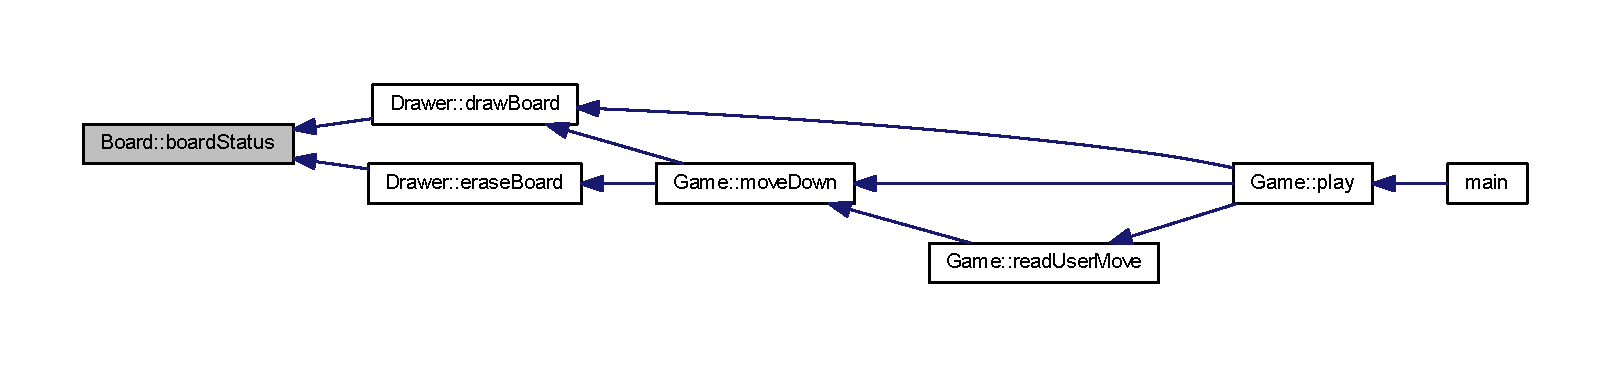
\includegraphics[width=350pt]{class_board_ac96b4da16e8dc266b39772f2da3fd7e2_icgraph}
\end{center}
\end{figure}
\mbox{\Hypertarget{class_board_a902cd3b288be772ba6b7abc6a822afea}\label{class_board_a902cd3b288be772ba6b7abc6a822afea}} 
\index{Board@{Board}!entry\+Coord@{entry\+Coord}}
\index{entry\+Coord@{entry\+Coord}!Board@{Board}}
\subsubsection{\texorpdfstring{entry\+Coord()}{entryCoord()}}
{\footnotesize\ttfamily \mbox{\hyperlink{struct_coord}{Coord}} Board\+::entry\+Coord (\begin{DoxyParamCaption}{ }\end{DoxyParamCaption}) const\hspace{0.3cm}{\ttfamily [inline]}}



진입 지점을 리턴한다 



tetris\+\_\+board.\+h 파일의 180 번째 라인에서 정의되었습니다.


\begin{DoxyCode}
181     \{
182         \textcolor{keywordflow}{return} \mbox{\hyperlink{class_board_a51d0b870dfe79367034bdda967e63a82}{entryPoint}};
183     \}
\end{DoxyCode}
\mbox{\Hypertarget{class_board_a888725ae3b1177a60a8f77299c1c939a}\label{class_board_a888725ae3b1177a60a8f77299c1c939a}} 
\index{Board@{Board}!get\+Height@{get\+Height}}
\index{get\+Height@{get\+Height}!Board@{Board}}
\subsubsection{\texorpdfstring{get\+Height()}{getHeight()}}
{\footnotesize\ttfamily int Board\+::get\+Height (\begin{DoxyParamCaption}{ }\end{DoxyParamCaption}) const\hspace{0.3cm}{\ttfamily [inline]}}



보드의 높이를 리턴한다 



tetris\+\_\+board.\+h 파일의 85 번째 라인에서 정의되었습니다.


\begin{DoxyCode}
86     \{
87         \textcolor{keywordflow}{return} \mbox{\hyperlink{class_board_a37b65287f3b416ed31b0f15cfd9b3f7c}{height}};
88     \}
\end{DoxyCode}
\mbox{\Hypertarget{class_board_a31bdad2985e3b4857a383dd2da8e8e27}\label{class_board_a31bdad2985e3b4857a383dd2da8e8e27}} 
\index{Board@{Board}!get\+Width@{get\+Width}}
\index{get\+Width@{get\+Width}!Board@{Board}}
\subsubsection{\texorpdfstring{get\+Width()}{getWidth()}}
{\footnotesize\ttfamily int Board\+::get\+Width (\begin{DoxyParamCaption}{ }\end{DoxyParamCaption}) const\hspace{0.3cm}{\ttfamily [inline]}}



보드의 너비를 리턴한다 



tetris\+\_\+board.\+h 파일의 79 번째 라인에서 정의되었습니다.


\begin{DoxyCode}
80     \{
81         \textcolor{keywordflow}{return} \mbox{\hyperlink{class_board_a5c5b64d99e3c653c425206d2babf2f97}{width}};
82     \}
\end{DoxyCode}
\mbox{\Hypertarget{class_board_a61ff9b1284e5c3e1214a780361ed650b}\label{class_board_a61ff9b1284e5c3e1214a780361ed650b}} 
\index{Board@{Board}!is\+Blocked@{is\+Blocked}}
\index{is\+Blocked@{is\+Blocked}!Board@{Board}}
\subsubsection{\texorpdfstring{is\+Blocked()}{isBlocked()}\hspace{0.1cm}{\footnotesize\ttfamily [1/2]}}
{\footnotesize\ttfamily bool Board\+::is\+Blocked (\begin{DoxyParamCaption}\item[{const \mbox{\hyperlink{struct_coord}{Coord}} \&}]{dest }\end{DoxyParamCaption}) const\hspace{0.3cm}{\ttfamily [inline]}, {\ttfamily [private]}}



좌표에 해당하는 자리에 이미 블럭이 있는지를 리턴 



tetris\+\_\+board.\+h 파일의 33 번째 라인에서 정의되었습니다.


\begin{DoxyCode}
34     \{
35         \textcolor{comment}{// 좌표와 배열 subscript 사이에는 반대 관계가 존재함에 유의}
36         \textcolor{keywordflow}{return} \mbox{\hyperlink{class_board_ad26aada4f19d2ca0c7bd534e8f466b6b}{board}}[dest.\mbox{\hyperlink{struct_coord_a214166cca70cef7dda9201689c3e81ab}{y}}][dest.\mbox{\hyperlink{struct_coord_a696eaa744360fc791d0e3b331c549dbe}{x}}].occupied == \textcolor{keyword}{true};   
37     \}
\end{DoxyCode}
이 함수를 호출하는 함수들에 대한 그래프입니다.\+:
\nopagebreak
\begin{figure}[H]
\begin{center}
\leavevmode
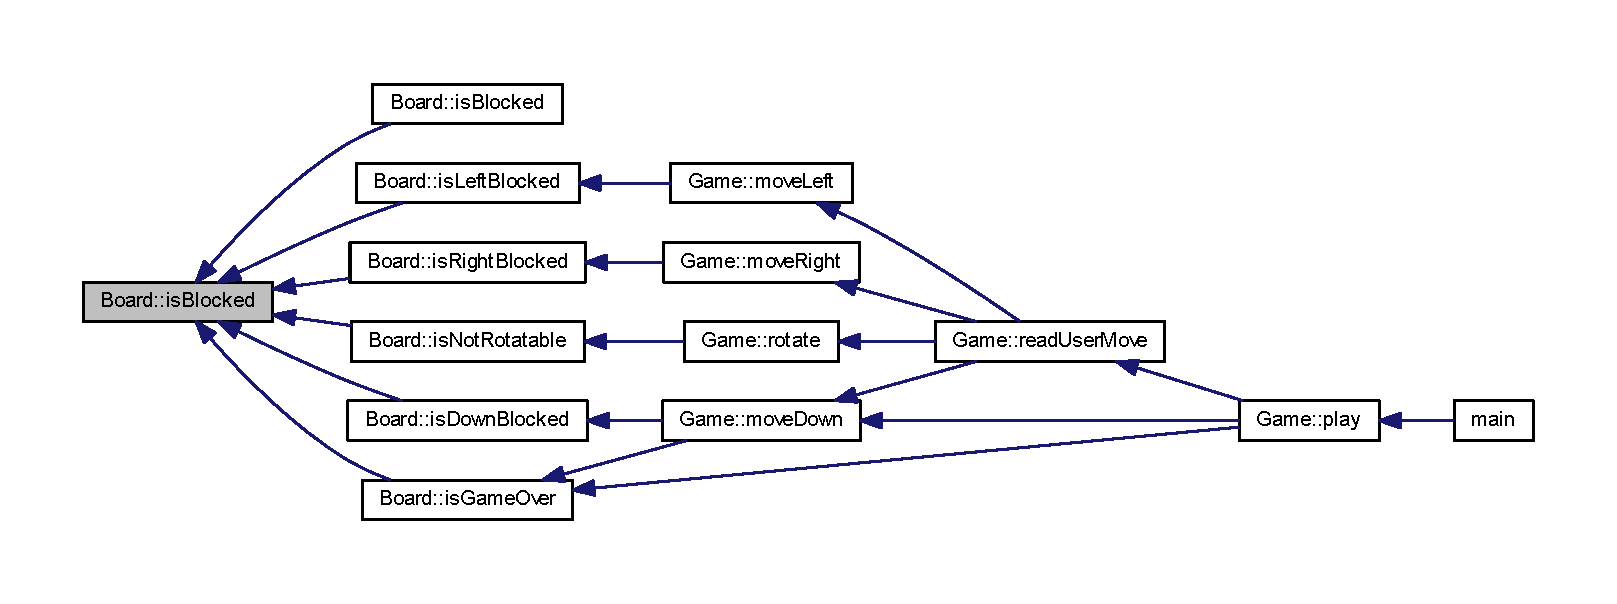
\includegraphics[width=350pt]{class_board_a61ff9b1284e5c3e1214a780361ed650b_icgraph}
\end{center}
\end{figure}
\mbox{\Hypertarget{class_board_a1ba0d2a44e1469738220b5ff7dfda6fc}\label{class_board_a1ba0d2a44e1469738220b5ff7dfda6fc}} 
\index{Board@{Board}!is\+Blocked@{is\+Blocked}}
\index{is\+Blocked@{is\+Blocked}!Board@{Board}}
\subsubsection{\texorpdfstring{is\+Blocked()}{isBlocked()}\hspace{0.1cm}{\footnotesize\ttfamily [2/2]}}
{\footnotesize\ttfamily bool Board\+::is\+Blocked (\begin{DoxyParamCaption}\item[{const \mbox{\hyperlink{struct_coord}{Coord}} \&}]{curr\+Pos,  }\item[{const \mbox{\hyperlink{class_block_aca5d951639f113e2ebd7856209d6b9ab}{Block\+::\+Block\+Shape}} \&}]{block\+Shape }\end{DoxyParamCaption}) const\hspace{0.3cm}{\ttfamily [inline]}, {\ttfamily [private]}}



해당하는 자리가 막혀있는지를 리턴 

현 위치와 현재 회전 상태를 읽어, 블럭의 자리에 다른 블럭이 막혀있는지를 리턴 
\begin{DoxyParams}{매개변수}
{\em curr\+Pos} & \+: 현재 좌표 \\
\hline
{\em block\+Shape} & \+: 현재 회전 상태에 따른 블럭 모양 \\
\hline
\end{DoxyParams}


tetris\+\_\+board.\+h 파일의 50 번째 라인에서 정의되었습니다.


\begin{DoxyCode}
51     \{
52         \textcolor{keywordflow}{for} (\textcolor{keyword}{auto} & x : blockShape)
53         \{
54             \mbox{\hyperlink{struct_coord}{Coord}} temp = currPos + x;
55             \textcolor{comment}{// 좌우 순서 중요(순서 변경 시 array out of bound 예외 발생)}
56             \textcolor{keywordflow}{if} (!\mbox{\hyperlink{class_board_a5df9c4c18c53b8029e0a080e5e089732}{isValid}}(temp) || \mbox{\hyperlink{class_board_a61ff9b1284e5c3e1214a780361ed650b}{isBlocked}}(temp))
57                 \textcolor{keywordflow}{return} \textcolor{keyword}{true};
58         \}
59         \textcolor{keywordflow}{return} \textcolor{keyword}{false};
60     \}
\end{DoxyCode}
이 함수 내부에서 호출하는 함수들에 대한 그래프입니다.\+:
\nopagebreak
\begin{figure}[H]
\begin{center}
\leavevmode
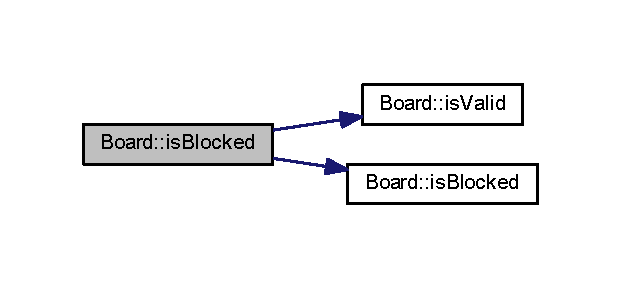
\includegraphics[width=298pt]{class_board_a1ba0d2a44e1469738220b5ff7dfda6fc_cgraph}
\end{center}
\end{figure}
\mbox{\Hypertarget{class_board_ad617ae22e46d1a62ed33592b20e00b44}\label{class_board_ad617ae22e46d1a62ed33592b20e00b44}} 
\index{Board@{Board}!is\+Down\+Blocked@{is\+Down\+Blocked}}
\index{is\+Down\+Blocked@{is\+Down\+Blocked}!Board@{Board}}
\subsubsection{\texorpdfstring{is\+Down\+Blocked()}{isDownBlocked()}}
{\footnotesize\ttfamily bool Board\+::is\+Down\+Blocked (\begin{DoxyParamCaption}\item[{const \mbox{\hyperlink{class_block_handler}{Block\+Handler}} \&}]{handler }\end{DoxyParamCaption}) const\hspace{0.3cm}{\ttfamily [inline]}}



현재 블럭의 아래가 막혀 있는 지를 리턴 



tetris\+\_\+board.\+h 파일의 105 번째 라인에서 정의되었습니다.


\begin{DoxyCode}
106     \{
107         \mbox{\hyperlink{struct_coord}{Coord}} temp(handler.\mbox{\hyperlink{class_block_handler_a11bd634fdc179446f9c6751e2394999e}{currPos}}.\mbox{\hyperlink{struct_coord_a696eaa744360fc791d0e3b331c549dbe}{x}}, handler.\mbox{\hyperlink{class_block_handler_a11bd634fdc179446f9c6751e2394999e}{currPos}}.\mbox{\hyperlink{struct_coord_a214166cca70cef7dda9201689c3e81ab}{y}} + 1);
108         \textcolor{keywordflow}{return} \mbox{\hyperlink{class_board_a61ff9b1284e5c3e1214a780361ed650b}{isBlocked}}(temp, handler.\mbox{\hyperlink{class_block_handler_ab57212ded2552ab5559d278c8538c454}{blk}}->getBlockInfo());
109     \}
\end{DoxyCode}
이 함수 내부에서 호출하는 함수들에 대한 그래프입니다.\+:
\nopagebreak
\begin{figure}[H]
\begin{center}
\leavevmode
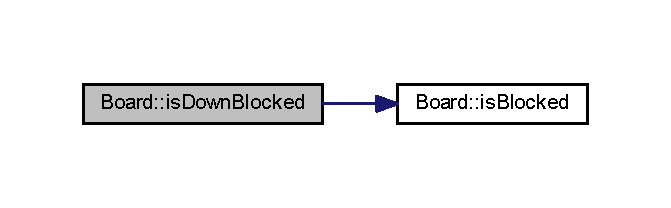
\includegraphics[width=322pt]{class_board_ad617ae22e46d1a62ed33592b20e00b44_cgraph}
\end{center}
\end{figure}
이 함수를 호출하는 함수들에 대한 그래프입니다.\+:
\nopagebreak
\begin{figure}[H]
\begin{center}
\leavevmode
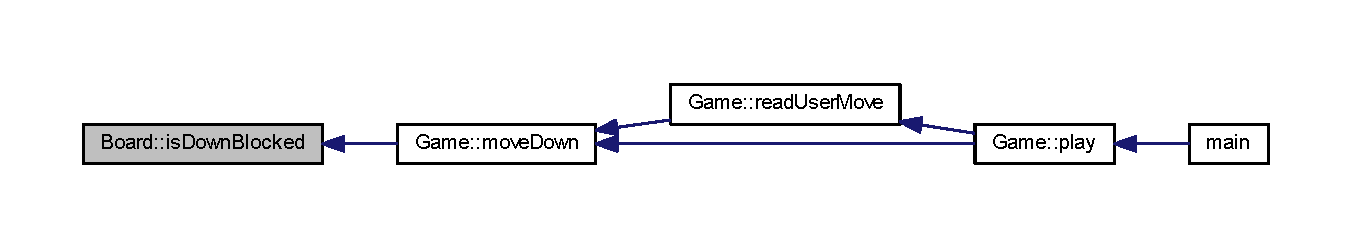
\includegraphics[width=350pt]{class_board_ad617ae22e46d1a62ed33592b20e00b44_icgraph}
\end{center}
\end{figure}
\mbox{\Hypertarget{class_board_a538ca2c02fbccf3af07ed3c821d9a736}\label{class_board_a538ca2c02fbccf3af07ed3c821d9a736}} 
\index{Board@{Board}!is\+Game\+Over@{is\+Game\+Over}}
\index{is\+Game\+Over@{is\+Game\+Over}!Board@{Board}}
\subsubsection{\texorpdfstring{is\+Game\+Over()}{isGameOver()}}
{\footnotesize\ttfamily bool Board\+::is\+Game\+Over (\begin{DoxyParamCaption}\item[{const \mbox{\hyperlink{class_block_handler}{Block\+Handler}} \&}]{handler }\end{DoxyParamCaption}) const\hspace{0.3cm}{\ttfamily [inline]}}



현재 블럭이 보드에 진입 가능한지를 리턴 



tetris\+\_\+board.\+h 파일의 118 번째 라인에서 정의되었습니다.


\begin{DoxyCode}
119     \{
120         \textcolor{keywordflow}{return} \mbox{\hyperlink{class_board_a61ff9b1284e5c3e1214a780361ed650b}{isBlocked}}(\mbox{\hyperlink{class_board_a51d0b870dfe79367034bdda967e63a82}{entryPoint}}, handler.\mbox{\hyperlink{class_block_handler_ab57212ded2552ab5559d278c8538c454}{blk}}->getBlockInfo());
121     \}
\end{DoxyCode}
이 함수 내부에서 호출하는 함수들에 대한 그래프입니다.\+:
\nopagebreak
\begin{figure}[H]
\begin{center}
\leavevmode
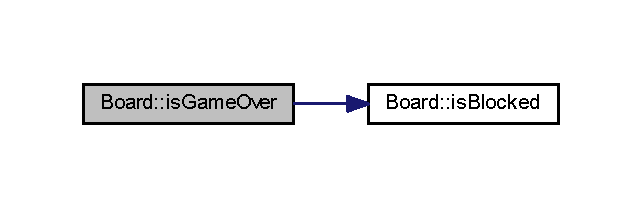
\includegraphics[width=308pt]{class_board_a538ca2c02fbccf3af07ed3c821d9a736_cgraph}
\end{center}
\end{figure}
이 함수를 호출하는 함수들에 대한 그래프입니다.\+:
\nopagebreak
\begin{figure}[H]
\begin{center}
\leavevmode
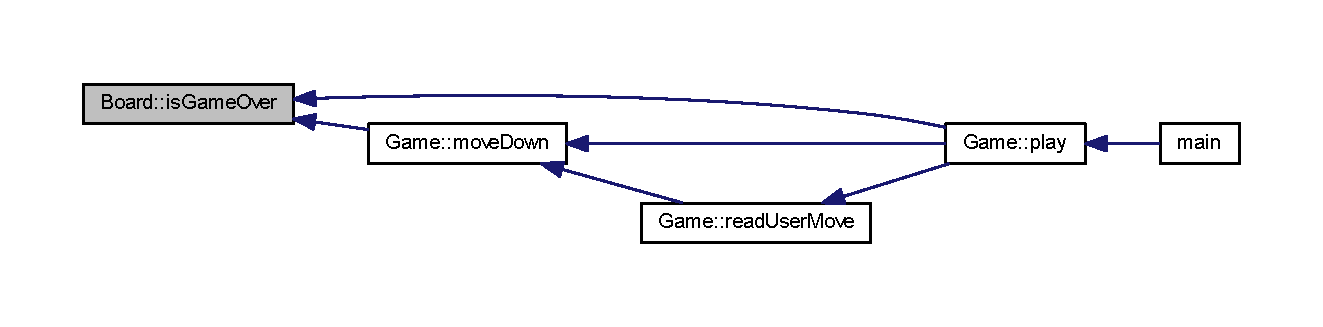
\includegraphics[width=350pt]{class_board_a538ca2c02fbccf3af07ed3c821d9a736_icgraph}
\end{center}
\end{figure}
\mbox{\Hypertarget{class_board_a5545704e21b5f7447eb9ffe014954cb3}\label{class_board_a5545704e21b5f7447eb9ffe014954cb3}} 
\index{Board@{Board}!is\+Left\+Blocked@{is\+Left\+Blocked}}
\index{is\+Left\+Blocked@{is\+Left\+Blocked}!Board@{Board}}
\subsubsection{\texorpdfstring{is\+Left\+Blocked()}{isLeftBlocked()}}
{\footnotesize\ttfamily bool Board\+::is\+Left\+Blocked (\begin{DoxyParamCaption}\item[{const \mbox{\hyperlink{class_block_handler}{Block\+Handler}} \&}]{handler }\end{DoxyParamCaption}) const\hspace{0.3cm}{\ttfamily [inline]}}



현재 블럭의 왼쪽이 막혀 있는 지를 리턴 



tetris\+\_\+board.\+h 파일의 91 번째 라인에서 정의되었습니다.


\begin{DoxyCode}
92     \{
93         \mbox{\hyperlink{struct_coord}{Coord}} temp(handler.\mbox{\hyperlink{class_block_handler_a11bd634fdc179446f9c6751e2394999e}{currPos}}.\mbox{\hyperlink{struct_coord_a696eaa744360fc791d0e3b331c549dbe}{x}} - 1, handler.\mbox{\hyperlink{class_block_handler_a11bd634fdc179446f9c6751e2394999e}{currPos}}.\mbox{\hyperlink{struct_coord_a214166cca70cef7dda9201689c3e81ab}{y}}); \textcolor{comment}{// 현 위치를 왼쪽으로 1칸 옮긴 임시
       위치 생성}
94         \textcolor{keywordflow}{return} \mbox{\hyperlink{class_board_a61ff9b1284e5c3e1214a780361ed650b}{isBlocked}}(temp, handler.\mbox{\hyperlink{class_block_handler_ab57212ded2552ab5559d278c8538c454}{blk}}->getBlockInfo());  \textcolor{comment}{// 임시 위치가 막혀 있는지를 리턴}
95     \}
\end{DoxyCode}
이 함수 내부에서 호출하는 함수들에 대한 그래프입니다.\+:
\nopagebreak
\begin{figure}[H]
\begin{center}
\leavevmode
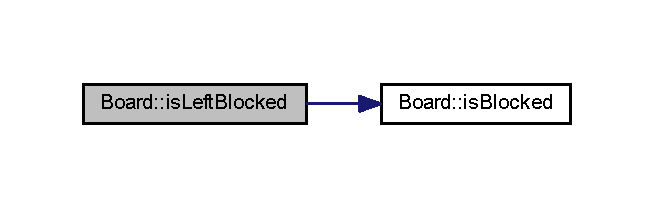
\includegraphics[width=314pt]{class_board_a5545704e21b5f7447eb9ffe014954cb3_cgraph}
\end{center}
\end{figure}
이 함수를 호출하는 함수들에 대한 그래프입니다.\+:
\nopagebreak
\begin{figure}[H]
\begin{center}
\leavevmode
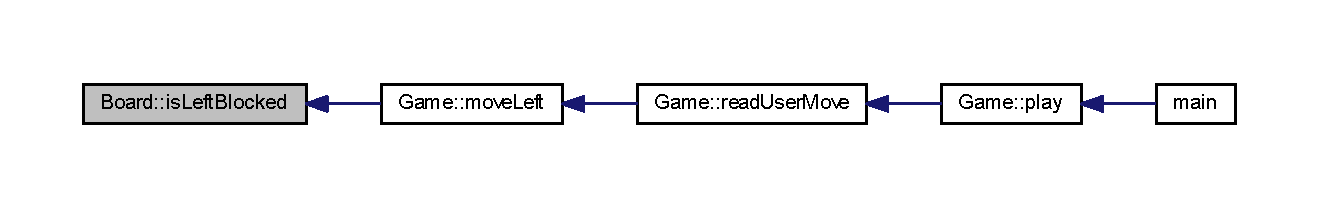
\includegraphics[width=350pt]{class_board_a5545704e21b5f7447eb9ffe014954cb3_icgraph}
\end{center}
\end{figure}
\mbox{\Hypertarget{class_board_a4b84310dd1ac3a08a3180361508a43e3}\label{class_board_a4b84310dd1ac3a08a3180361508a43e3}} 
\index{Board@{Board}!is\+Not\+Rotatable@{is\+Not\+Rotatable}}
\index{is\+Not\+Rotatable@{is\+Not\+Rotatable}!Board@{Board}}
\subsubsection{\texorpdfstring{is\+Not\+Rotatable()}{isNotRotatable()}}
{\footnotesize\ttfamily bool Board\+::is\+Not\+Rotatable (\begin{DoxyParamCaption}\item[{const \mbox{\hyperlink{class_block_handler}{Block\+Handler}} \&}]{handler }\end{DoxyParamCaption}) const\hspace{0.3cm}{\ttfamily [inline]}}



현재 블럭이 회전 불가능한지를 리턴 



tetris\+\_\+board.\+h 파일의 112 번째 라인에서 정의되었습니다.


\begin{DoxyCode}
113     \{
114         \textcolor{keywordflow}{return} \mbox{\hyperlink{class_board_a61ff9b1284e5c3e1214a780361ed650b}{isBlocked}}(handler.\mbox{\hyperlink{class_block_handler_a11bd634fdc179446f9c6751e2394999e}{currPos}}, handler.\mbox{\hyperlink{class_block_handler_ab57212ded2552ab5559d278c8538c454}{blk}}->getNextBlockInfo()); \textcolor{comment}{// 현재 블럭을
       회전했을 경우 막히는지를 리턴}
115     \}
\end{DoxyCode}
이 함수 내부에서 호출하는 함수들에 대한 그래프입니다.\+:
\nopagebreak
\begin{figure}[H]
\begin{center}
\leavevmode
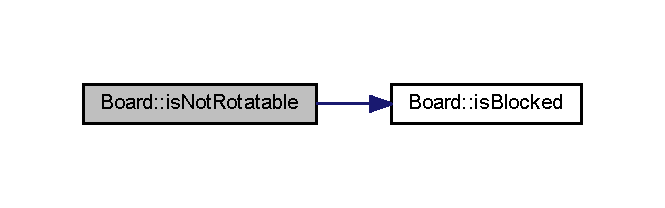
\includegraphics[width=319pt]{class_board_a4b84310dd1ac3a08a3180361508a43e3_cgraph}
\end{center}
\end{figure}
이 함수를 호출하는 함수들에 대한 그래프입니다.\+:
\nopagebreak
\begin{figure}[H]
\begin{center}
\leavevmode
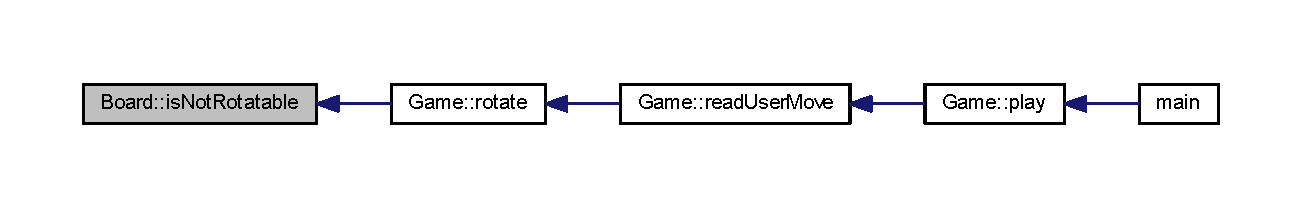
\includegraphics[width=350pt]{class_board_a4b84310dd1ac3a08a3180361508a43e3_icgraph}
\end{center}
\end{figure}
\mbox{\Hypertarget{class_board_ad38cdb8757f58a32b5747e2b7e0be277}\label{class_board_ad38cdb8757f58a32b5747e2b7e0be277}} 
\index{Board@{Board}!is\+Right\+Blocked@{is\+Right\+Blocked}}
\index{is\+Right\+Blocked@{is\+Right\+Blocked}!Board@{Board}}
\subsubsection{\texorpdfstring{is\+Right\+Blocked()}{isRightBlocked()}}
{\footnotesize\ttfamily bool Board\+::is\+Right\+Blocked (\begin{DoxyParamCaption}\item[{const \mbox{\hyperlink{class_block_handler}{Block\+Handler}} \&}]{handler }\end{DoxyParamCaption}) const\hspace{0.3cm}{\ttfamily [inline]}}



현재 블럭의 오른쪽이 막혀 있는 지를 리턴 



tetris\+\_\+board.\+h 파일의 98 번째 라인에서 정의되었습니다.


\begin{DoxyCode}
99     \{
100         \mbox{\hyperlink{struct_coord}{Coord}} temp(handler.\mbox{\hyperlink{class_block_handler_a11bd634fdc179446f9c6751e2394999e}{currPos}}.\mbox{\hyperlink{struct_coord_a696eaa744360fc791d0e3b331c549dbe}{x}} + 1, handler.\mbox{\hyperlink{class_block_handler_a11bd634fdc179446f9c6751e2394999e}{currPos}}.\mbox{\hyperlink{struct_coord_a214166cca70cef7dda9201689c3e81ab}{y}});
101         \textcolor{keywordflow}{return} \mbox{\hyperlink{class_board_a61ff9b1284e5c3e1214a780361ed650b}{isBlocked}}(temp, handler.\mbox{\hyperlink{class_block_handler_ab57212ded2552ab5559d278c8538c454}{blk}}->getBlockInfo());
102     \}
\end{DoxyCode}
이 함수 내부에서 호출하는 함수들에 대한 그래프입니다.\+:
\nopagebreak
\begin{figure}[H]
\begin{center}
\leavevmode
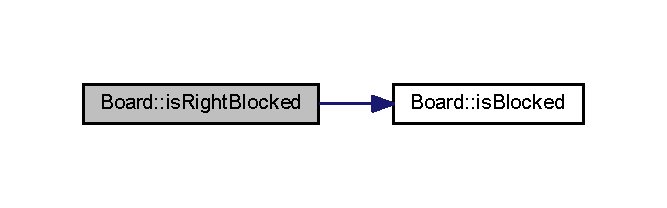
\includegraphics[width=320pt]{class_board_ad38cdb8757f58a32b5747e2b7e0be277_cgraph}
\end{center}
\end{figure}
이 함수를 호출하는 함수들에 대한 그래프입니다.\+:
\nopagebreak
\begin{figure}[H]
\begin{center}
\leavevmode
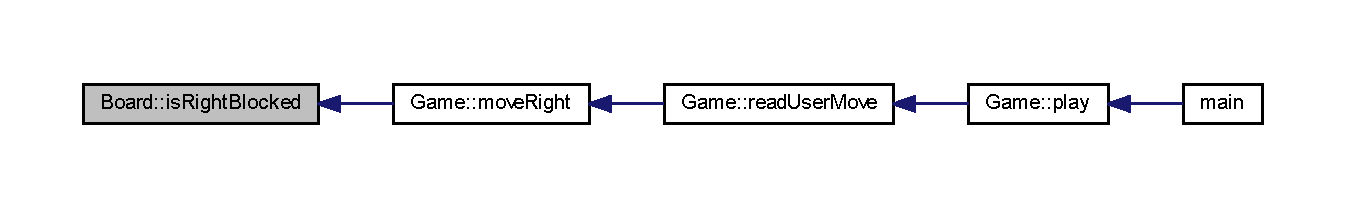
\includegraphics[width=350pt]{class_board_ad38cdb8757f58a32b5747e2b7e0be277_icgraph}
\end{center}
\end{figure}
\mbox{\Hypertarget{class_board_a5df9c4c18c53b8029e0a080e5e089732}\label{class_board_a5df9c4c18c53b8029e0a080e5e089732}} 
\index{Board@{Board}!is\+Valid@{is\+Valid}}
\index{is\+Valid@{is\+Valid}!Board@{Board}}
\subsubsection{\texorpdfstring{is\+Valid()}{isValid()}}
{\footnotesize\ttfamily bool Board\+::is\+Valid (\begin{DoxyParamCaption}\item[{const \mbox{\hyperlink{struct_coord}{Coord}} \&}]{dest }\end{DoxyParamCaption}) const\hspace{0.3cm}{\ttfamily [inline]}, {\ttfamily [private]}}



tetris\+\_\+board.\+h 파일의 39 번째 라인에서 정의되었습니다.


\begin{DoxyCode}
40     \{
41         \textcolor{keywordflow}{return} !(dest.\mbox{\hyperlink{struct_coord_a696eaa744360fc791d0e3b331c549dbe}{x}} < 0 || dest.\mbox{\hyperlink{struct_coord_a696eaa744360fc791d0e3b331c549dbe}{x}} >= \mbox{\hyperlink{class_board_a5c5b64d99e3c653c425206d2babf2f97}{width}} || dest.\mbox{\hyperlink{struct_coord_a214166cca70cef7dda9201689c3e81ab}{y}} < 0 || dest.\mbox{\hyperlink{struct_coord_a214166cca70cef7dda9201689c3e81ab}{y}} >= 
      \mbox{\hyperlink{class_board_a37b65287f3b416ed31b0f15cfd9b3f7c}{height}});
42     \}
\end{DoxyCode}
이 함수를 호출하는 함수들에 대한 그래프입니다.\+:
\nopagebreak
\begin{figure}[H]
\begin{center}
\leavevmode
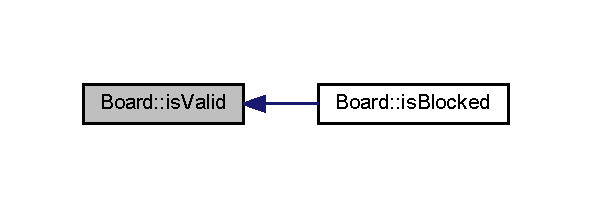
\includegraphics[width=284pt]{class_board_a5df9c4c18c53b8029e0a080e5e089732_icgraph}
\end{center}
\end{figure}
\mbox{\Hypertarget{class_board_a06e5188ef352fc5c0e3957895cef6a89}\label{class_board_a06e5188ef352fc5c0e3957895cef6a89}} 
\index{Board@{Board}!update\+Board@{update\+Board}}
\index{update\+Board@{update\+Board}!Board@{Board}}
\subsubsection{\texorpdfstring{update\+Board()}{updateBoard()}}
{\footnotesize\ttfamily void Board\+::update\+Board (\begin{DoxyParamCaption}\item[{const \mbox{\hyperlink{class_block_handler}{Block\+Handler}} \&}]{handler }\end{DoxyParamCaption})\hspace{0.3cm}{\ttfamily [inline]}}



블럭이 끝에 도달했을 때, 이를 보드에 기록한다. 줄이 꽉찼다면 보드를 새로 고친다. 



tetris\+\_\+board.\+h 파일의 124 번째 라인에서 정의되었습니다.


\begin{DoxyCode}
125     \{
126         \textcolor{comment}{// 현재 블럭의 정보를 보드에 반영한다.}
127         \mbox{\hyperlink{class_block_ad054b4ac51df79aa910040b2a2fdf7b5}{Block::Color}} currentBlockColor = handler.\mbox{\hyperlink{class_block_handler_ab57212ded2552ab5559d278c8538c454}{blk}}->getColor();
128         \textcolor{keywordflow}{for} (\textcolor{keyword}{auto} & blkInfo : handler.\mbox{\hyperlink{class_block_handler_ab57212ded2552ab5559d278c8538c454}{blk}}->getBlockInfo())
129         \{
130             \textcolor{comment}{// 좌표와 배열 subscript 사이에는 반대 관계가 존재함에 유의}
131             \mbox{\hyperlink{class_board_ad26aada4f19d2ca0c7bd534e8f466b6b}{board}}[handler.\mbox{\hyperlink{class_block_handler_a11bd634fdc179446f9c6751e2394999e}{currPos}}.\mbox{\hyperlink{struct_coord_a214166cca70cef7dda9201689c3e81ab}{y}} + blkInfo.y][handler.\mbox{\hyperlink{class_block_handler_a11bd634fdc179446f9c6751e2394999e}{currPos}}.
      \mbox{\hyperlink{struct_coord_a696eaa744360fc791d0e3b331c549dbe}{x}} + blkInfo.x].occupied = \textcolor{keyword}{true};
132             \mbox{\hyperlink{class_board_ad26aada4f19d2ca0c7bd534e8f466b6b}{board}}[handler.\mbox{\hyperlink{class_block_handler_a11bd634fdc179446f9c6751e2394999e}{currPos}}.\mbox{\hyperlink{struct_coord_a214166cca70cef7dda9201689c3e81ab}{y}} + blkInfo.y][handler.\mbox{\hyperlink{class_block_handler_a11bd634fdc179446f9c6751e2394999e}{currPos}}.
      \mbox{\hyperlink{struct_coord_a696eaa744360fc791d0e3b331c549dbe}{x}} + blkInfo.x].color = currentBlockColor;
133         \}
134 
135         \textcolor{comment}{// 꽉찬 줄이 있는지 검사한다.}
136         std::vector<bool> lineChecker;
137         \textcolor{keywordtype}{int} count;
138         \textcolor{keywordtype}{bool} refreshFlag = \textcolor{keyword}{false};
139         \textcolor{comment}{// 보드의 위에서부터 아래로 꽉찬 줄을 검사한다.}
140         \textcolor{keywordflow}{for} (\textcolor{keywordtype}{int} i = \mbox{\hyperlink{class_board_a37b65287f3b416ed31b0f15cfd9b3f7c}{height}} - 1; i >= 0; --i)
141         \{
142             count = 0;
143             \textcolor{comment}{// 이번 줄의 찬 자리를 센다.}
144             \textcolor{keywordflow}{for} (\textcolor{keywordtype}{int} j = 0; j < \mbox{\hyperlink{class_board_a5c5b64d99e3c653c425206d2babf2f97}{width}}; ++j)
145             \{
146                 \textcolor{keywordflow}{if} (\mbox{\hyperlink{class_board_ad26aada4f19d2ca0c7bd534e8f466b6b}{board}}[i][j].occupied == \textcolor{keyword}{true})
147                     ++count;
148                 \textcolor{keywordflow}{else}
149                     \textcolor{keywordflow}{break};
150             \}
151 
152             \textcolor{comment}{// 줄이 꽉찼다면 false, 반대라면 true를 push한다.}
153             \textcolor{keywordflow}{if} (count == \mbox{\hyperlink{class_board_a5c5b64d99e3c653c425206d2babf2f97}{width}})
154             \{
155                 lineChecker.push\_back(\textcolor{keyword}{false});
156                 refreshFlag = \textcolor{keyword}{true};
157             \}
158             \textcolor{keywordflow}{else}
159                 lineChecker.push\_back(\textcolor{keyword}{true});
160         \}
161 
162         \textcolor{comment}{// 만약 꽉찬 줄이 하나라도 있다면, 보드를 새로 고친다.}
163         \textcolor{keywordflow}{if} (refreshFlag == \textcolor{keyword}{true})
164         \{
165             \textcolor{comment}{// 새 보드를 생성하여 기존 보드로부터 정보를 받되, 꽉 찬 줄은 스킵한다.}
166             \mbox{\hyperlink{class_board_a84bf794bc185e31e333b78bb003c4bc3}{BoardType}} newBoard \{\};
167             \textcolor{keywordtype}{int} j = lineChecker.size() - 1;
168             \textcolor{keywordflow}{for} (\textcolor{keywordtype}{int} i = lineChecker.size() - 1; i >= 0; --i)
169                 \textcolor{keywordflow}{if} (lineChecker[lineChecker.size() - 1 - i] == \textcolor{keyword}{true})
170                 \{
171                     \textcolor{keywordflow}{for} (\textcolor{keywordtype}{int} k = 0; k < \mbox{\hyperlink{class_board_a5c5b64d99e3c653c425206d2babf2f97}{width}}; ++k)
172                         newBoard[j][k] = \mbox{\hyperlink{class_board_ad26aada4f19d2ca0c7bd534e8f466b6b}{board}}[i][k];
173                     --j;
174                 \}
175             \mbox{\hyperlink{class_board_ad26aada4f19d2ca0c7bd534e8f466b6b}{board}} = newBoard;
176         \}
177 \}
\end{DoxyCode}
이 함수를 호출하는 함수들에 대한 그래프입니다.\+:
\nopagebreak
\begin{figure}[H]
\begin{center}
\leavevmode
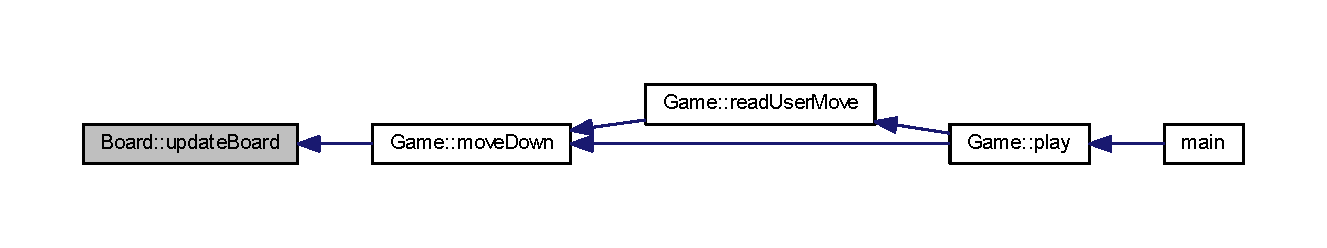
\includegraphics[width=350pt]{class_board_a06e5188ef352fc5c0e3957895cef6a89_icgraph}
\end{center}
\end{figure}


\subsection{멤버 데이터 문서화}
\mbox{\Hypertarget{class_board_ad26aada4f19d2ca0c7bd534e8f466b6b}\label{class_board_ad26aada4f19d2ca0c7bd534e8f466b6b}} 
\index{Board@{Board}!board@{board}}
\index{board@{board}!Board@{Board}}
\subsubsection{\texorpdfstring{board}{board}}
{\footnotesize\ttfamily \mbox{\hyperlink{class_board_a84bf794bc185e31e333b78bb003c4bc3}{Board\+Type}} Board\+::board \{\}\hspace{0.3cm}{\ttfamily [private]}}



보드(\mbox{\hyperlink{struct_board_1_1cell_info}{cell\+Info}} 2차원 배열) 



tetris\+\_\+board.\+h 파일의 29 번째 라인에서 정의되었습니다.

\mbox{\Hypertarget{class_board_a51d0b870dfe79367034bdda967e63a82}\label{class_board_a51d0b870dfe79367034bdda967e63a82}} 
\index{Board@{Board}!entry\+Point@{entry\+Point}}
\index{entry\+Point@{entry\+Point}!Board@{Board}}
\subsubsection{\texorpdfstring{entry\+Point}{entryPoint}}
{\footnotesize\ttfamily const \mbox{\hyperlink{struct_coord}{Coord}} Board\+::entry\+Point\hspace{0.3cm}{\ttfamily [private]}}



보드 내 블럭의 진입 지점 -\/ width와 height 다음에 선언되어야 한다 



tetris\+\_\+board.\+h 파일의 30 번째 라인에서 정의되었습니다.

\mbox{\Hypertarget{class_board_a37b65287f3b416ed31b0f15cfd9b3f7c}\label{class_board_a37b65287f3b416ed31b0f15cfd9b3f7c}} 
\index{Board@{Board}!height@{height}}
\index{height@{height}!Board@{Board}}
\subsubsection{\texorpdfstring{height}{height}}
{\footnotesize\ttfamily const int Board\+::height\hspace{0.3cm}{\ttfamily [private]}}



보드의 높이(10) 



tetris\+\_\+board.\+h 파일의 28 번째 라인에서 정의되었습니다.

\mbox{\Hypertarget{class_board_a5c5b64d99e3c653c425206d2babf2f97}\label{class_board_a5c5b64d99e3c653c425206d2babf2f97}} 
\index{Board@{Board}!width@{width}}
\index{width@{width}!Board@{Board}}
\subsubsection{\texorpdfstring{width}{width}}
{\footnotesize\ttfamily const int Board\+::width\hspace{0.3cm}{\ttfamily [private]}}



보드의 너비(25) 



tetris\+\_\+board.\+h 파일의 27 번째 라인에서 정의되었습니다.



이 클래스에 대한 문서화 페이지는 다음의 파일로부터 생성되었습니다.\+:\begin{DoxyCompactItemize}
\item 
\mbox{\hyperlink{tetris__board_8h}{tetris\+\_\+board.\+h}}\end{DoxyCompactItemize}

\hypertarget{struct_board_1_1cell_info}{}\section{Board\+:\+:cell\+Info 구조체 참조}
\label{struct_board_1_1cell_info}\index{Board\+::cell\+Info@{Board\+::cell\+Info}}


보드 내 각 셀에 대한 정보(채워져 있나 여부, 채운 블럭의 색상) 저장.  




{\ttfamily \#include $<$tetris\+\_\+board.\+h$>$}



Board\+:\+:cell\+Info에 대한 협력 다이어그램\+:
\nopagebreak
\begin{figure}[H]
\begin{center}
\leavevmode
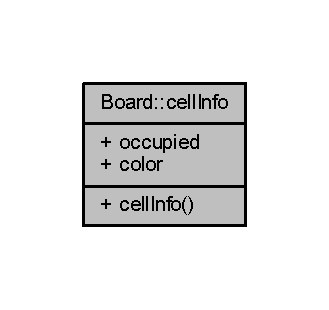
\includegraphics[width=158pt]{struct_board_1_1cell_info__coll__graph}
\end{center}
\end{figure}
\subsection*{Public 멤버 함수}
\begin{DoxyCompactItemize}
\item 
\mbox{\hyperlink{struct_board_1_1cell_info_a6912555905168decac5c8dd1fba998a9}{cell\+Info}} ()
\end{DoxyCompactItemize}
\subsection*{Public 속성}
\begin{DoxyCompactItemize}
\item 
bool \mbox{\hyperlink{struct_board_1_1cell_info_a518ee0af8b662d092a1e4dffefadf27c}{occupied}}
\item 
\mbox{\hyperlink{class_block_ad054b4ac51df79aa910040b2a2fdf7b5}{Block\+::\+Color}} \mbox{\hyperlink{struct_board_1_1cell_info_ac4e0ca21aefe0f000144641e5eb6698d}{color}}
\end{DoxyCompactItemize}


\subsection{상세한 설명}
보드 내 각 셀에 대한 정보(채워져 있나 여부, 채운 블럭의 색상) 저장. 

tetris\+\_\+board.\+h 파일의 18 번째 라인에서 정의되었습니다.



\subsection{생성자 \& 소멸자 문서화}
\mbox{\Hypertarget{struct_board_1_1cell_info_a6912555905168decac5c8dd1fba998a9}\label{struct_board_1_1cell_info_a6912555905168decac5c8dd1fba998a9}} 
\index{Board\+::cell\+Info@{Board\+::cell\+Info}!cell\+Info@{cell\+Info}}
\index{cell\+Info@{cell\+Info}!Board\+::cell\+Info@{Board\+::cell\+Info}}
\subsubsection{\texorpdfstring{cell\+Info()}{cellInfo()}}
{\footnotesize\ttfamily Board\+::cell\+Info\+::cell\+Info (\begin{DoxyParamCaption}{ }\end{DoxyParamCaption})\hspace{0.3cm}{\ttfamily [inline]}}



tetris\+\_\+board.\+h 파일의 22 번째 라인에서 정의되었습니다.


\begin{DoxyCode}
22 : \mbox{\hyperlink{struct_board_1_1cell_info_a518ee0af8b662d092a1e4dffefadf27c}{occupied}}(\textcolor{keyword}{false}), \mbox{\hyperlink{struct_board_1_1cell_info_ac4e0ca21aefe0f000144641e5eb6698d}{color}}(Block::Color::WHITE) \{\}
\end{DoxyCode}


\subsection{멤버 데이터 문서화}
\mbox{\Hypertarget{struct_board_1_1cell_info_ac4e0ca21aefe0f000144641e5eb6698d}\label{struct_board_1_1cell_info_ac4e0ca21aefe0f000144641e5eb6698d}} 
\index{Board\+::cell\+Info@{Board\+::cell\+Info}!color@{color}}
\index{color@{color}!Board\+::cell\+Info@{Board\+::cell\+Info}}
\subsubsection{\texorpdfstring{color}{color}}
{\footnotesize\ttfamily \mbox{\hyperlink{class_block_ad054b4ac51df79aa910040b2a2fdf7b5}{Block\+::\+Color}} Board\+::cell\+Info\+::color}



tetris\+\_\+board.\+h 파일의 21 번째 라인에서 정의되었습니다.

\mbox{\Hypertarget{struct_board_1_1cell_info_a518ee0af8b662d092a1e4dffefadf27c}\label{struct_board_1_1cell_info_a518ee0af8b662d092a1e4dffefadf27c}} 
\index{Board\+::cell\+Info@{Board\+::cell\+Info}!occupied@{occupied}}
\index{occupied@{occupied}!Board\+::cell\+Info@{Board\+::cell\+Info}}
\subsubsection{\texorpdfstring{occupied}{occupied}}
{\footnotesize\ttfamily bool Board\+::cell\+Info\+::occupied}



tetris\+\_\+board.\+h 파일의 20 번째 라인에서 정의되었습니다.



이 구조체에 대한 문서화 페이지는 다음의 파일로부터 생성되었습니다.\+:\begin{DoxyCompactItemize}
\item 
\mbox{\hyperlink{tetris__board_8h}{tetris\+\_\+board.\+h}}\end{DoxyCompactItemize}

\hypertarget{struct_coord}{}\section{Coord 구조체 참조}
\label{struct_coord}\index{Coord@{Coord}}


\mbox{\hyperlink{class_board}{Board}} 내의 좌표와 \mbox{\hyperlink{class_block}{Block}} 모양의 좌표 형식 정보 표현  




{\ttfamily \#include $<$tetris\+\_\+block.\+h$>$}



Coord에 대한 협력 다이어그램\+:
\nopagebreak
\begin{figure}[H]
\begin{center}
\leavevmode
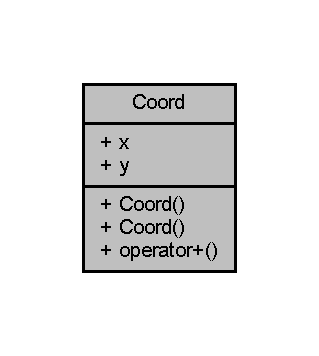
\includegraphics[width=153pt]{struct_coord__coll__graph}
\end{center}
\end{figure}
\subsection*{Public 멤버 함수}
\begin{DoxyCompactItemize}
\item 
\mbox{\hyperlink{struct_coord_a46e518631fa539ebb8a7f2a5b59fd483}{Coord}} ()=delete
\item 
\mbox{\hyperlink{struct_coord_ab01ff8e569cc417d7c669007e12a5fa1}{Coord}} (int xpos, int ypos)
\item 
\mbox{\hyperlink{struct_coord}{Coord}} \mbox{\hyperlink{struct_coord_ad564b77330c90986e1586d2d04aad6f9}{operator+}} (const \mbox{\hyperlink{struct_coord}{Coord}} \&operand) const
\end{DoxyCompactItemize}
\subsection*{Public 속성}
\begin{DoxyCompactItemize}
\item 
int \mbox{\hyperlink{struct_coord_a696eaa744360fc791d0e3b331c549dbe}{x}}
\item 
int \mbox{\hyperlink{struct_coord_a214166cca70cef7dda9201689c3e81ab}{y}}
\end{DoxyCompactItemize}


\subsection{상세한 설명}
\mbox{\hyperlink{class_board}{Board}} 내의 좌표와 \mbox{\hyperlink{class_block}{Block}} 모양의 좌표 형식 정보 표현 

\mbox{\hyperlink{class_board}{Board}} 내에서의 좌표를 (열, 행) 순서로 표현한다. \mbox{\hyperlink{class_block}{Block}} 모양의 좌표 형식 정보를 (열, 행) 순서로 표현한다. 

tetris\+\_\+block.\+h 파일의 9 번째 라인에서 정의되었습니다.



\subsection{생성자 \& 소멸자 문서화}
\mbox{\Hypertarget{struct_coord_a46e518631fa539ebb8a7f2a5b59fd483}\label{struct_coord_a46e518631fa539ebb8a7f2a5b59fd483}} 
\index{Coord@{Coord}!Coord@{Coord}}
\index{Coord@{Coord}!Coord@{Coord}}
\subsubsection{\texorpdfstring{Coord()}{Coord()}\hspace{0.1cm}{\footnotesize\ttfamily [1/2]}}
{\footnotesize\ttfamily Coord\+::\+Coord (\begin{DoxyParamCaption}{ }\end{DoxyParamCaption})\hspace{0.3cm}{\ttfamily [delete]}}

이 함수를 호출하는 함수들에 대한 그래프입니다.\+:
\nopagebreak
\begin{figure}[H]
\begin{center}
\leavevmode
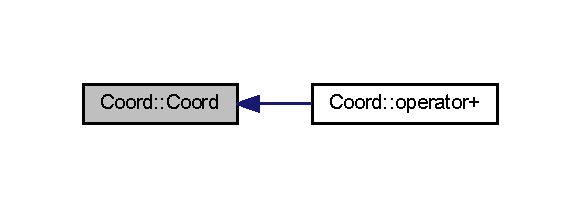
\includegraphics[width=279pt]{struct_coord_a46e518631fa539ebb8a7f2a5b59fd483_icgraph}
\end{center}
\end{figure}
\mbox{\Hypertarget{struct_coord_ab01ff8e569cc417d7c669007e12a5fa1}\label{struct_coord_ab01ff8e569cc417d7c669007e12a5fa1}} 
\index{Coord@{Coord}!Coord@{Coord}}
\index{Coord@{Coord}!Coord@{Coord}}
\subsubsection{\texorpdfstring{Coord()}{Coord()}\hspace{0.1cm}{\footnotesize\ttfamily [2/2]}}
{\footnotesize\ttfamily Coord\+::\+Coord (\begin{DoxyParamCaption}\item[{int}]{xpos,  }\item[{int}]{ypos }\end{DoxyParamCaption})\hspace{0.3cm}{\ttfamily [inline]}}



tetris\+\_\+block.\+h 파일의 14 번째 라인에서 정의되었습니다.


\begin{DoxyCode}
14 : \mbox{\hyperlink{struct_coord_a696eaa744360fc791d0e3b331c549dbe}{x}}(xpos), \mbox{\hyperlink{struct_coord_a214166cca70cef7dda9201689c3e81ab}{y}}(ypos) \{\}
\end{DoxyCode}


\subsection{멤버 함수 문서화}
\mbox{\Hypertarget{struct_coord_ad564b77330c90986e1586d2d04aad6f9}\label{struct_coord_ad564b77330c90986e1586d2d04aad6f9}} 
\index{Coord@{Coord}!operator+@{operator+}}
\index{operator+@{operator+}!Coord@{Coord}}
\subsubsection{\texorpdfstring{operator+()}{operator+()}}
{\footnotesize\ttfamily \mbox{\hyperlink{struct_coord}{Coord}} Coord\+::operator+ (\begin{DoxyParamCaption}\item[{const \mbox{\hyperlink{struct_coord}{Coord}} \&}]{operand }\end{DoxyParamCaption}) const\hspace{0.3cm}{\ttfamily [inline]}}



tetris\+\_\+block.\+h 파일의 15 번째 라인에서 정의되었습니다.


\begin{DoxyCode}
16     \{
17         \textcolor{keywordflow}{return} \mbox{\hyperlink{struct_coord_a46e518631fa539ebb8a7f2a5b59fd483}{Coord}}(\mbox{\hyperlink{struct_coord_a696eaa744360fc791d0e3b331c549dbe}{x}} + operand.\mbox{\hyperlink{struct_coord_a696eaa744360fc791d0e3b331c549dbe}{x}}, \mbox{\hyperlink{struct_coord_a214166cca70cef7dda9201689c3e81ab}{y}} + operand.\mbox{\hyperlink{struct_coord_a214166cca70cef7dda9201689c3e81ab}{y}});
18     \}
\end{DoxyCode}
이 함수 내부에서 호출하는 함수들에 대한 그래프입니다.\+:
\nopagebreak
\begin{figure}[H]
\begin{center}
\leavevmode
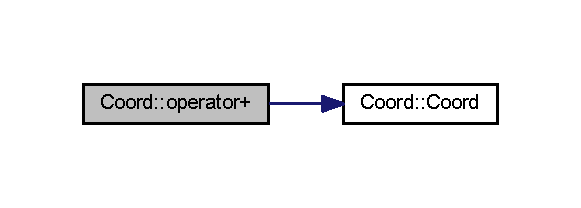
\includegraphics[width=279pt]{struct_coord_ad564b77330c90986e1586d2d04aad6f9_cgraph}
\end{center}
\end{figure}


\subsection{멤버 데이터 문서화}
\mbox{\Hypertarget{struct_coord_a696eaa744360fc791d0e3b331c549dbe}\label{struct_coord_a696eaa744360fc791d0e3b331c549dbe}} 
\index{Coord@{Coord}!x@{x}}
\index{x@{x}!Coord@{Coord}}
\subsubsection{\texorpdfstring{x}{x}}
{\footnotesize\ttfamily int Coord\+::x}



tetris\+\_\+block.\+h 파일의 11 번째 라인에서 정의되었습니다.

\mbox{\Hypertarget{struct_coord_a214166cca70cef7dda9201689c3e81ab}\label{struct_coord_a214166cca70cef7dda9201689c3e81ab}} 
\index{Coord@{Coord}!y@{y}}
\index{y@{y}!Coord@{Coord}}
\subsubsection{\texorpdfstring{y}{y}}
{\footnotesize\ttfamily int Coord\+::y}



tetris\+\_\+block.\+h 파일의 12 번째 라인에서 정의되었습니다.



이 구조체에 대한 문서화 페이지는 다음의 파일로부터 생성되었습니다.\+:\begin{DoxyCompactItemize}
\item 
\mbox{\hyperlink{tetris__block_8h}{tetris\+\_\+block.\+h}}\end{DoxyCompactItemize}

\hypertarget{class_drawer}{}\section{Drawer 클래스 참조}
\label{class_drawer}\index{Drawer@{Drawer}}


화면에 게임을 출력하는 클래스  




{\ttfamily \#include $<$tetris\+\_\+drawer.\+h$>$}



Drawer에 대한 협력 다이어그램\+:
\nopagebreak
\begin{figure}[H]
\begin{center}
\leavevmode
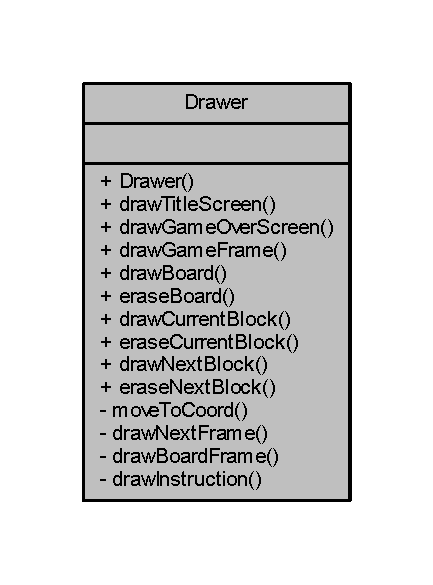
\includegraphics[width=208pt]{class_drawer__coll__graph}
\end{center}
\end{figure}
\subsection*{Public 멤버 함수}
\begin{DoxyCompactItemize}
\item 
\mbox{\hyperlink{class_drawer_a7daabfaadc8a076a71f5f09b0a88f4bb}{Drawer}} ()
\item 
void \mbox{\hyperlink{class_drawer_ad87ca95db3cafee6f005e297e2c6d4de}{draw\+Title\+Screen}} () const
\begin{DoxyCompactList}\small\item\em 타이틀 화면을 그림 \end{DoxyCompactList}\item 
void \mbox{\hyperlink{class_drawer_a57ec099eb46c93f20d9221a2244dd9a7}{draw\+Game\+Over\+Screen}} (const \mbox{\hyperlink{class_board}{Board}} \&bd) const
\begin{DoxyCompactList}\small\item\em 게임오버 화면을 그림 \end{DoxyCompactList}\item 
void \mbox{\hyperlink{class_drawer_a9f5e10f6175710be253244d6f80ebcf7}{draw\+Game\+Frame}} () const
\begin{DoxyCompactList}\small\item\em 게임 플레이에 필요한 프레임들을 그림 \end{DoxyCompactList}\item 
void \mbox{\hyperlink{class_drawer_af26df40487cb2de033887b5342d94b5a}{draw\+Board}} (const \mbox{\hyperlink{class_board}{Board}} \&bd) const
\begin{DoxyCompactList}\small\item\em 보드를 그림 \end{DoxyCompactList}\item 
void \mbox{\hyperlink{class_drawer_ad8b55aff1fbf975536ef3d995d3a4526}{erase\+Board}} (const \mbox{\hyperlink{class_board}{Board}} \&bd) const
\begin{DoxyCompactList}\small\item\em 보드를 지움 \end{DoxyCompactList}\item 
void \mbox{\hyperlink{class_drawer_acef9be5772c0a3bdbae4f01d851e60f1}{draw\+Current\+Block}} (const \mbox{\hyperlink{class_block_handler}{Block\+Handler}} \&handle) const
\begin{DoxyCompactList}\small\item\em 현재 블럭을 그림 \end{DoxyCompactList}\item 
void \mbox{\hyperlink{class_drawer_a513de5ba9d65771ed21918a90cd70afa}{erase\+Current\+Block}} (const \mbox{\hyperlink{class_block_handler}{Block\+Handler}} \&handle) const
\begin{DoxyCompactList}\small\item\em 현재 블럭을 지움 \end{DoxyCompactList}\item 
void \mbox{\hyperlink{class_drawer_a6d8f74fa5fae96990547abb2521b5432}{draw\+Next\+Block}} (const \mbox{\hyperlink{class_block_handler}{Block\+Handler}} \&handle) const
\begin{DoxyCompactList}\small\item\em 다음 블럭을 그림 \end{DoxyCompactList}\item 
void \mbox{\hyperlink{class_drawer_a3110e80f9256176373f0580788e69037}{erase\+Next\+Block}} (const \mbox{\hyperlink{class_block_handler}{Block\+Handler}} \&handle) const
\begin{DoxyCompactList}\small\item\em 다음 블럭을 지움 \end{DoxyCompactList}\end{DoxyCompactItemize}
\subsection*{Private 멤버 함수}
\begin{DoxyCompactItemize}
\item 
void \mbox{\hyperlink{class_drawer_ac1a96e007c07cab2e36a7c78484ee9a6}{move\+To\+Coord}} (int x, int y) const
\begin{DoxyCompactList}\small\item\em 해당 좌표로 커서를 이동시킴 \end{DoxyCompactList}\item 
void \mbox{\hyperlink{class_drawer_a2deae79fb268b41b72693d005cdf2178}{draw\+Next\+Frame}} () const
\begin{DoxyCompactList}\small\item\em 다음 블럭을 나타낼 자리에 프레임을 그림 \end{DoxyCompactList}\item 
void \mbox{\hyperlink{class_drawer_a72d01f53fc2c5ff15763dcd76a9b9395}{draw\+Board\+Frame}} () const
\begin{DoxyCompactList}\small\item\em 보드 프레임을 그림 \end{DoxyCompactList}\item 
void \mbox{\hyperlink{class_drawer_a4fb74bcad295250c519bb848dd48b0de}{draw\+Instruction}} () const
\begin{DoxyCompactList}\small\item\em 게임 플레이 방법을 그림 \end{DoxyCompactList}\end{DoxyCompactItemize}


\subsection{상세한 설명}
화면에 게임을 출력하는 클래스 

tetris\+\_\+drawer.\+h 파일의 18 번째 라인에서 정의되었습니다.



\subsection{생성자 \& 소멸자 문서화}
\mbox{\Hypertarget{class_drawer_a7daabfaadc8a076a71f5f09b0a88f4bb}\label{class_drawer_a7daabfaadc8a076a71f5f09b0a88f4bb}} 
\index{Drawer@{Drawer}!Drawer@{Drawer}}
\index{Drawer@{Drawer}!Drawer@{Drawer}}
\subsubsection{\texorpdfstring{Drawer()}{Drawer()}}
{\footnotesize\ttfamily Drawer\+::\+Drawer (\begin{DoxyParamCaption}{ }\end{DoxyParamCaption})\hspace{0.3cm}{\ttfamily [inline]}}



tetris\+\_\+drawer.\+h 파일의 83 번째 라인에서 정의되었습니다.


\begin{DoxyCode}
83 \{\}
\end{DoxyCode}


\subsection{멤버 함수 문서화}
\mbox{\Hypertarget{class_drawer_af26df40487cb2de033887b5342d94b5a}\label{class_drawer_af26df40487cb2de033887b5342d94b5a}} 
\index{Drawer@{Drawer}!draw\+Board@{draw\+Board}}
\index{draw\+Board@{draw\+Board}!Drawer@{Drawer}}
\subsubsection{\texorpdfstring{draw\+Board()}{drawBoard()}}
{\footnotesize\ttfamily void Drawer\+::draw\+Board (\begin{DoxyParamCaption}\item[{const \mbox{\hyperlink{class_board}{Board}} \&}]{bd }\end{DoxyParamCaption}) const\hspace{0.3cm}{\ttfamily [inline]}}



보드를 그림 



tetris\+\_\+drawer.\+h 파일의 135 번째 라인에서 정의되었습니다.


\begin{DoxyCode}
136     \{
137         \textcolor{keyword}{const} \mbox{\hyperlink{class_board_a84bf794bc185e31e333b78bb003c4bc3}{Board::BoardType}} & status = bd.\mbox{\hyperlink{class_board_ac96b4da16e8dc266b39772f2da3fd7e2}{boardStatus}}();
138         \textcolor{keywordflow}{for} (\textcolor{keywordtype}{int} i = 0; i < 25; ++i)
139             \textcolor{keywordflow}{for} (\textcolor{keywordtype}{int} j = 0; j < 10; ++j)
140                 \textcolor{keywordflow}{if} (status[i][j].occupied == \textcolor{keyword}{true})  \textcolor{comment}{// false 시 else문을 통해 std::cout << "  "; 을 사용하면 간혹 게임이
       매우 느려짐.}
141                 \{
142                     \mbox{\hyperlink{class_drawer_ac1a96e007c07cab2e36a7c78484ee9a6}{moveToCoord}}(\mbox{\hyperlink{tetris__drawer_8h_afe5fa4d0ad1820f448b83de84142af4d}{boardDrawCoord}}.\mbox{\hyperlink{struct_coord_a696eaa744360fc791d0e3b331c549dbe}{x}} + j * 2, 
      \mbox{\hyperlink{tetris__drawer_8h_afe5fa4d0ad1820f448b83de84142af4d}{boardDrawCoord}}.\mbox{\hyperlink{struct_coord_a214166cca70cef7dda9201689c3e81ab}{y}} + i);
143                     SetConsoleTextAttribute(GetStdHandle(STD\_OUTPUT\_HANDLE), static\_cast<WORD>(status[i][j]
      .color));
144                     std::cout << \textcolor{stringliteral}{"■"};
145                 \}
146     \}
\end{DoxyCode}
이 함수 내부에서 호출하는 함수들에 대한 그래프입니다.\+:
\nopagebreak
\begin{figure}[H]
\begin{center}
\leavevmode
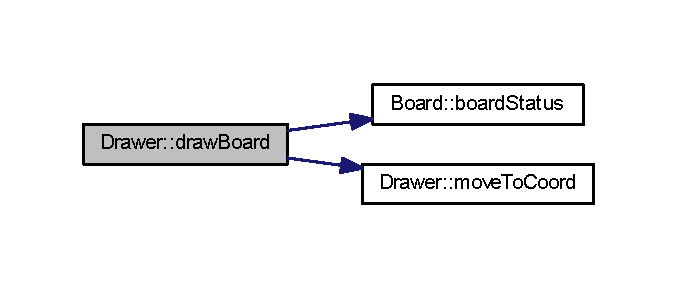
\includegraphics[width=325pt]{class_drawer_af26df40487cb2de033887b5342d94b5a_cgraph}
\end{center}
\end{figure}
이 함수를 호출하는 함수들에 대한 그래프입니다.\+:
\nopagebreak
\begin{figure}[H]
\begin{center}
\leavevmode
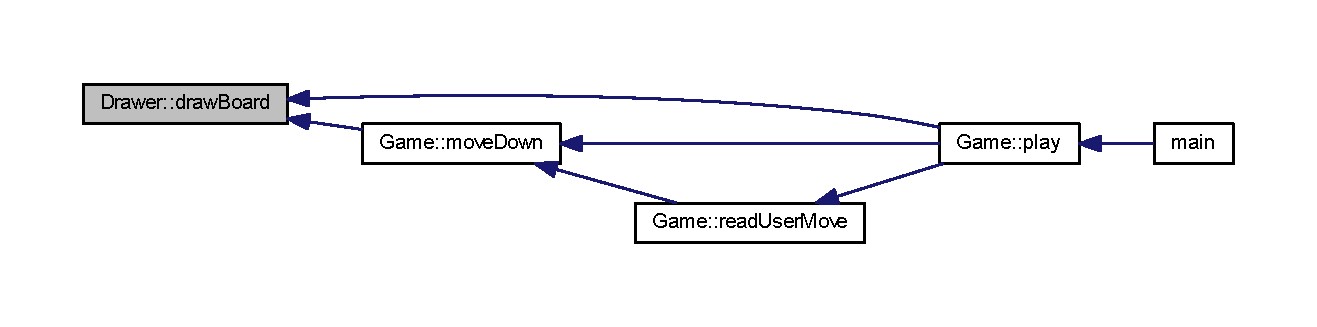
\includegraphics[width=350pt]{class_drawer_af26df40487cb2de033887b5342d94b5a_icgraph}
\end{center}
\end{figure}
\mbox{\Hypertarget{class_drawer_a72d01f53fc2c5ff15763dcd76a9b9395}\label{class_drawer_a72d01f53fc2c5ff15763dcd76a9b9395}} 
\index{Drawer@{Drawer}!draw\+Board\+Frame@{draw\+Board\+Frame}}
\index{draw\+Board\+Frame@{draw\+Board\+Frame}!Drawer@{Drawer}}
\subsubsection{\texorpdfstring{draw\+Board\+Frame()}{drawBoardFrame()}}
{\footnotesize\ttfamily void Drawer\+::draw\+Board\+Frame (\begin{DoxyParamCaption}{ }\end{DoxyParamCaption}) const\hspace{0.3cm}{\ttfamily [inline]}, {\ttfamily [private]}}



보드 프레임을 그림 



tetris\+\_\+drawer.\+h 파일의 51 번째 라인에서 정의되었습니다.


\begin{DoxyCode}
52     \{
53         \mbox{\hyperlink{class_drawer_ac1a96e007c07cab2e36a7c78484ee9a6}{moveToCoord}}(\mbox{\hyperlink{tetris__drawer_8h_a4dcd1769680ae6c150a2285edfeb9e1f}{boardFrameDrawCoord}}.\mbox{\hyperlink{struct_coord_a696eaa744360fc791d0e3b331c549dbe}{x}}, 
      \mbox{\hyperlink{tetris__drawer_8h_a4dcd1769680ae6c150a2285edfeb9e1f}{boardFrameDrawCoord}}.\mbox{\hyperlink{struct_coord_a214166cca70cef7dda9201689c3e81ab}{y}});
54         \textcolor{keywordflow}{for} (\textcolor{keywordtype}{int} i = 0; i < 12; ++i)
55             std::cout << \textcolor{stringliteral}{"▩"};
56         \textcolor{keywordflow}{for} (\textcolor{keywordtype}{int} i = \mbox{\hyperlink{tetris__drawer_8h_a4dcd1769680ae6c150a2285edfeb9e1f}{boardFrameDrawCoord}}.\mbox{\hyperlink{struct_coord_a214166cca70cef7dda9201689c3e81ab}{y}} + 1; i < 
      \mbox{\hyperlink{tetris__drawer_8h_a4dcd1769680ae6c150a2285edfeb9e1f}{boardFrameDrawCoord}}.\mbox{\hyperlink{struct_coord_a214166cca70cef7dda9201689c3e81ab}{y}} + 26; ++i)
57         \{
58             \mbox{\hyperlink{class_drawer_ac1a96e007c07cab2e36a7c78484ee9a6}{moveToCoord}}(\mbox{\hyperlink{tetris__drawer_8h_a4dcd1769680ae6c150a2285edfeb9e1f}{boardFrameDrawCoord}}.\mbox{\hyperlink{struct_coord_a696eaa744360fc791d0e3b331c549dbe}{x}}, i);
59             std::cout << \textcolor{stringliteral}{"▩"};
60             \mbox{\hyperlink{class_drawer_ac1a96e007c07cab2e36a7c78484ee9a6}{moveToCoord}}(\mbox{\hyperlink{tetris__drawer_8h_a4dcd1769680ae6c150a2285edfeb9e1f}{boardFrameDrawCoord}}.\mbox{\hyperlink{struct_coord_a696eaa744360fc791d0e3b331c549dbe}{x}} + 22, i);
61             std::cout << \textcolor{stringliteral}{"▩"};
62         \}
63         \mbox{\hyperlink{class_drawer_ac1a96e007c07cab2e36a7c78484ee9a6}{moveToCoord}}(\mbox{\hyperlink{tetris__drawer_8h_a4dcd1769680ae6c150a2285edfeb9e1f}{boardFrameDrawCoord}}.\mbox{\hyperlink{struct_coord_a696eaa744360fc791d0e3b331c549dbe}{x}}, 
      \mbox{\hyperlink{tetris__drawer_8h_a4dcd1769680ae6c150a2285edfeb9e1f}{boardFrameDrawCoord}}.\mbox{\hyperlink{struct_coord_a214166cca70cef7dda9201689c3e81ab}{y}} + 26);
64         \textcolor{keywordflow}{for} (\textcolor{keywordtype}{int} i = 0; i < 12; ++i)
65             std::cout << \textcolor{stringliteral}{"▩"};
66     \}
\end{DoxyCode}
이 함수 내부에서 호출하는 함수들에 대한 그래프입니다.\+:
\nopagebreak
\begin{figure}[H]
\begin{center}
\leavevmode
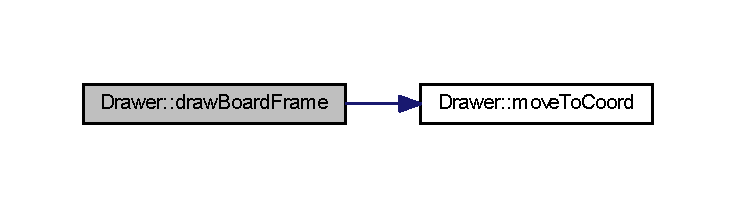
\includegraphics[width=350pt]{class_drawer_a72d01f53fc2c5ff15763dcd76a9b9395_cgraph}
\end{center}
\end{figure}
이 함수를 호출하는 함수들에 대한 그래프입니다.\+:
\nopagebreak
\begin{figure}[H]
\begin{center}
\leavevmode
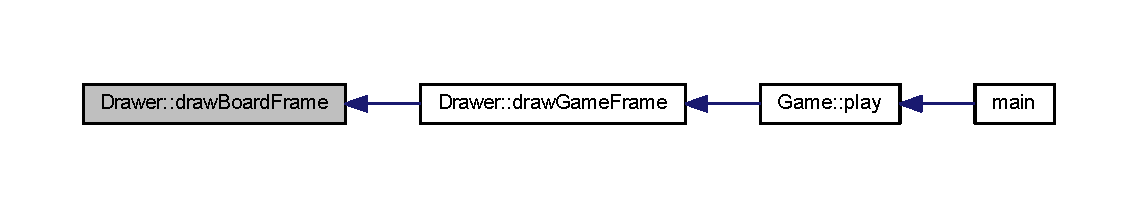
\includegraphics[width=350pt]{class_drawer_a72d01f53fc2c5ff15763dcd76a9b9395_icgraph}
\end{center}
\end{figure}
\mbox{\Hypertarget{class_drawer_acef9be5772c0a3bdbae4f01d851e60f1}\label{class_drawer_acef9be5772c0a3bdbae4f01d851e60f1}} 
\index{Drawer@{Drawer}!draw\+Current\+Block@{draw\+Current\+Block}}
\index{draw\+Current\+Block@{draw\+Current\+Block}!Drawer@{Drawer}}
\subsubsection{\texorpdfstring{draw\+Current\+Block()}{drawCurrentBlock()}}
{\footnotesize\ttfamily void Drawer\+::draw\+Current\+Block (\begin{DoxyParamCaption}\item[{const \mbox{\hyperlink{class_block_handler}{Block\+Handler}} \&}]{handle }\end{DoxyParamCaption}) const\hspace{0.3cm}{\ttfamily [inline]}}



현재 블럭을 그림 



tetris\+\_\+drawer.\+h 파일의 162 번째 라인에서 정의되었습니다.


\begin{DoxyCode}
163     \{
164         \mbox{\hyperlink{class_block_ad054b4ac51df79aa910040b2a2fdf7b5}{Block::Color}} currentBlockColor = handle.\mbox{\hyperlink{class_block_handler_ab57212ded2552ab5559d278c8538c454}{blk}}->getColor();
165         SetConsoleTextAttribute(GetStdHandle(STD\_OUTPUT\_HANDLE), static\_cast<WORD>(currentBlockColor));
166         \textcolor{keywordflow}{for} (\textcolor{keyword}{auto} & cellInfo : handle.\mbox{\hyperlink{class_block_handler_ab57212ded2552ab5559d278c8538c454}{blk}}->getBlockInfo())
167         \{
168             \mbox{\hyperlink{struct_coord}{Coord}} temp = handle.\mbox{\hyperlink{class_block_handler_a11bd634fdc179446f9c6751e2394999e}{currPos}} + cellInfo;
169             \mbox{\hyperlink{class_drawer_ac1a96e007c07cab2e36a7c78484ee9a6}{moveToCoord}}(\mbox{\hyperlink{tetris__drawer_8h_afe5fa4d0ad1820f448b83de84142af4d}{boardDrawCoord}}.\mbox{\hyperlink{struct_coord_a696eaa744360fc791d0e3b331c549dbe}{x}} + temp.\mbox{\hyperlink{struct_coord_a696eaa744360fc791d0e3b331c549dbe}{x}} * 2, 
      \mbox{\hyperlink{tetris__drawer_8h_afe5fa4d0ad1820f448b83de84142af4d}{boardDrawCoord}}.\mbox{\hyperlink{struct_coord_a214166cca70cef7dda9201689c3e81ab}{y}} + temp.\mbox{\hyperlink{struct_coord_a214166cca70cef7dda9201689c3e81ab}{y}});
170             std::cout << \textcolor{stringliteral}{"■"};
171         \}
172     \}
\end{DoxyCode}
이 함수 내부에서 호출하는 함수들에 대한 그래프입니다.\+:
\nopagebreak
\begin{figure}[H]
\begin{center}
\leavevmode
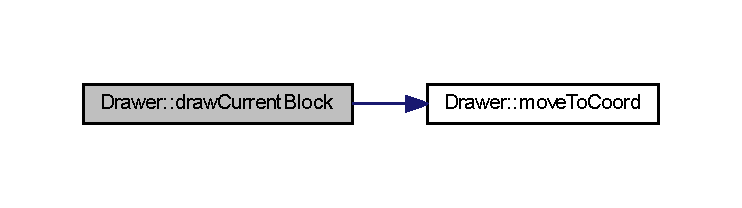
\includegraphics[width=350pt]{class_drawer_acef9be5772c0a3bdbae4f01d851e60f1_cgraph}
\end{center}
\end{figure}
이 함수를 호출하는 함수들에 대한 그래프입니다.\+:
\nopagebreak
\begin{figure}[H]
\begin{center}
\leavevmode
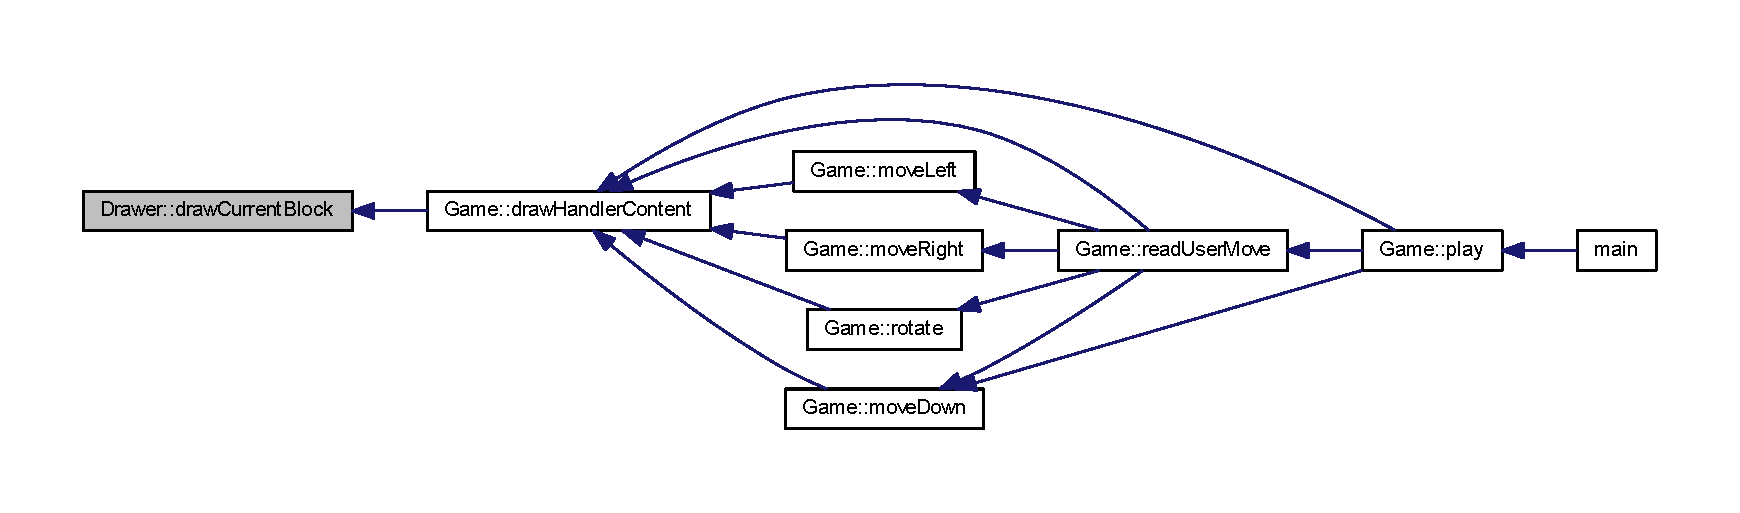
\includegraphics[width=350pt]{class_drawer_acef9be5772c0a3bdbae4f01d851e60f1_icgraph}
\end{center}
\end{figure}
\mbox{\Hypertarget{class_drawer_a9f5e10f6175710be253244d6f80ebcf7}\label{class_drawer_a9f5e10f6175710be253244d6f80ebcf7}} 
\index{Drawer@{Drawer}!draw\+Game\+Frame@{draw\+Game\+Frame}}
\index{draw\+Game\+Frame@{draw\+Game\+Frame}!Drawer@{Drawer}}
\subsubsection{\texorpdfstring{draw\+Game\+Frame()}{drawGameFrame()}}
{\footnotesize\ttfamily void Drawer\+::draw\+Game\+Frame (\begin{DoxyParamCaption}{ }\end{DoxyParamCaption}) const\hspace{0.3cm}{\ttfamily [inline]}}



게임 플레이에 필요한 프레임들을 그림 



tetris\+\_\+drawer.\+h 파일의 126 번째 라인에서 정의되었습니다.


\begin{DoxyCode}
127     \{
128         system(\textcolor{stringliteral}{"cls"});
129         \mbox{\hyperlink{class_drawer_a2deae79fb268b41b72693d005cdf2178}{drawNextFrame}}();
130         \mbox{\hyperlink{class_drawer_a72d01f53fc2c5ff15763dcd76a9b9395}{drawBoardFrame}}();
131         \mbox{\hyperlink{class_drawer_a4fb74bcad295250c519bb848dd48b0de}{drawInstruction}}();
132     \}
\end{DoxyCode}
이 함수 내부에서 호출하는 함수들에 대한 그래프입니다.\+:
\nopagebreak
\begin{figure}[H]
\begin{center}
\leavevmode
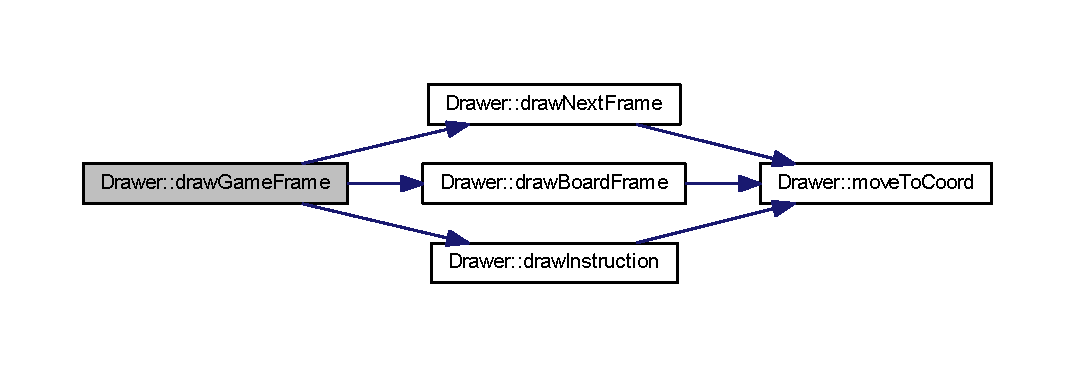
\includegraphics[width=350pt]{class_drawer_a9f5e10f6175710be253244d6f80ebcf7_cgraph}
\end{center}
\end{figure}
이 함수를 호출하는 함수들에 대한 그래프입니다.\+:
\nopagebreak
\begin{figure}[H]
\begin{center}
\leavevmode
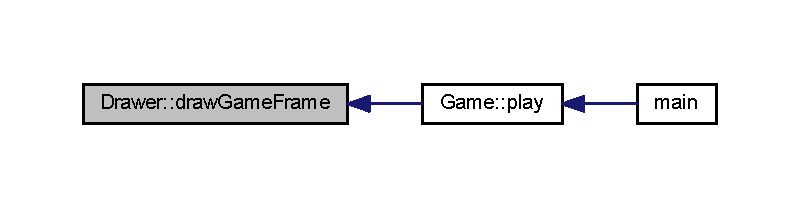
\includegraphics[width=350pt]{class_drawer_a9f5e10f6175710be253244d6f80ebcf7_icgraph}
\end{center}
\end{figure}
\mbox{\Hypertarget{class_drawer_a57ec099eb46c93f20d9221a2244dd9a7}\label{class_drawer_a57ec099eb46c93f20d9221a2244dd9a7}} 
\index{Drawer@{Drawer}!draw\+Game\+Over\+Screen@{draw\+Game\+Over\+Screen}}
\index{draw\+Game\+Over\+Screen@{draw\+Game\+Over\+Screen}!Drawer@{Drawer}}
\subsubsection{\texorpdfstring{draw\+Game\+Over\+Screen()}{drawGameOverScreen()}}
{\footnotesize\ttfamily void Drawer\+::draw\+Game\+Over\+Screen (\begin{DoxyParamCaption}\item[{const \mbox{\hyperlink{class_board}{Board}} \&}]{bd }\end{DoxyParamCaption}) const\hspace{0.3cm}{\ttfamily [inline]}}



게임오버 화면을 그림 



tetris\+\_\+drawer.\+h 파일의 111 번째 라인에서 정의되었습니다.


\begin{DoxyCode}
112     \{
113         SetConsoleTextAttribute(GetStdHandle(STD\_OUTPUT\_HANDLE), 0x7);
114         
115         \mbox{\hyperlink{class_drawer_ac1a96e007c07cab2e36a7c78484ee9a6}{moveToCoord}}(\mbox{\hyperlink{tetris__drawer_8h_afe5fa4d0ad1820f448b83de84142af4d}{boardDrawCoord}}.\mbox{\hyperlink{struct_coord_a696eaa744360fc791d0e3b331c549dbe}{x}}, \mbox{\hyperlink{tetris__drawer_8h_afe5fa4d0ad1820f448b83de84142af4d}{boardDrawCoord}}.
      \mbox{\hyperlink{struct_coord_a214166cca70cef7dda9201689c3e81ab}{y}} + 9);
116         std::cout << \textcolor{stringliteral}{"                    "}; \textcolor{comment}{// 20 spaces}
117         \mbox{\hyperlink{class_drawer_ac1a96e007c07cab2e36a7c78484ee9a6}{moveToCoord}}(\mbox{\hyperlink{tetris__drawer_8h_afe5fa4d0ad1820f448b83de84142af4d}{boardDrawCoord}}.\mbox{\hyperlink{struct_coord_a696eaa744360fc791d0e3b331c549dbe}{x}}, \mbox{\hyperlink{tetris__drawer_8h_afe5fa4d0ad1820f448b83de84142af4d}{boardDrawCoord}}.
      \mbox{\hyperlink{struct_coord_a214166cca70cef7dda9201689c3e81ab}{y}} + 10);
118         std::cout << \textcolor{stringliteral}{"  G A M E O V E R   "};
119         \mbox{\hyperlink{class_drawer_ac1a96e007c07cab2e36a7c78484ee9a6}{moveToCoord}}(\mbox{\hyperlink{tetris__drawer_8h_afe5fa4d0ad1820f448b83de84142af4d}{boardDrawCoord}}.\mbox{\hyperlink{struct_coord_a696eaa744360fc791d0e3b331c549dbe}{x}}, \mbox{\hyperlink{tetris__drawer_8h_afe5fa4d0ad1820f448b83de84142af4d}{boardDrawCoord}}.
      \mbox{\hyperlink{struct_coord_a214166cca70cef7dda9201689c3e81ab}{y}} + 11);
120         std::cout << \textcolor{stringliteral}{"                    "};
121         \mbox{\hyperlink{class_drawer_ac1a96e007c07cab2e36a7c78484ee9a6}{moveToCoord}}(0, 0);
122         Sleep(1000);
123     \}
\end{DoxyCode}
이 함수 내부에서 호출하는 함수들에 대한 그래프입니다.\+:
\nopagebreak
\begin{figure}[H]
\begin{center}
\leavevmode
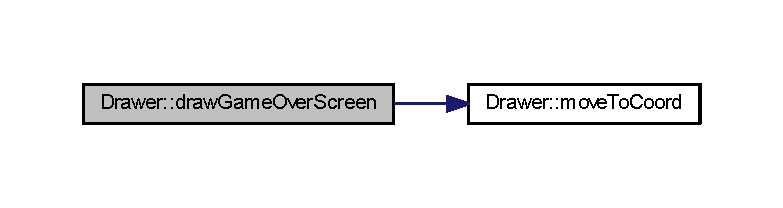
\includegraphics[width=350pt]{class_drawer_a57ec099eb46c93f20d9221a2244dd9a7_cgraph}
\end{center}
\end{figure}
이 함수를 호출하는 함수들에 대한 그래프입니다.\+:
\nopagebreak
\begin{figure}[H]
\begin{center}
\leavevmode
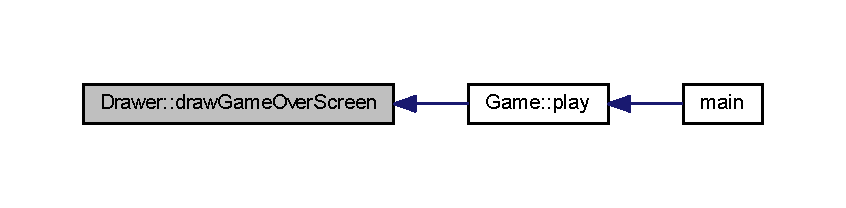
\includegraphics[width=350pt]{class_drawer_a57ec099eb46c93f20d9221a2244dd9a7_icgraph}
\end{center}
\end{figure}
\mbox{\Hypertarget{class_drawer_a4fb74bcad295250c519bb848dd48b0de}\label{class_drawer_a4fb74bcad295250c519bb848dd48b0de}} 
\index{Drawer@{Drawer}!draw\+Instruction@{draw\+Instruction}}
\index{draw\+Instruction@{draw\+Instruction}!Drawer@{Drawer}}
\subsubsection{\texorpdfstring{draw\+Instruction()}{drawInstruction()}}
{\footnotesize\ttfamily void Drawer\+::draw\+Instruction (\begin{DoxyParamCaption}{ }\end{DoxyParamCaption}) const\hspace{0.3cm}{\ttfamily [inline]}, {\ttfamily [private]}}



게임 플레이 방법을 그림 



tetris\+\_\+drawer.\+h 파일의 69 번째 라인에서 정의되었습니다.


\begin{DoxyCode}
70     \{
71         \mbox{\hyperlink{class_drawer_ac1a96e007c07cab2e36a7c78484ee9a6}{moveToCoord}}(\mbox{\hyperlink{tetris__drawer_8h_a19714d61f50f7fa80357eba4d88aa69d}{instructionDrawCoord}}.\mbox{\hyperlink{struct_coord_a696eaa744360fc791d0e3b331c549dbe}{x}}, 
      \mbox{\hyperlink{tetris__drawer_8h_a19714d61f50f7fa80357eba4d88aa69d}{instructionDrawCoord}}.\mbox{\hyperlink{struct_coord_a214166cca70cef7dda9201689c3e81ab}{y}});
72         std::cout << \textcolor{stringliteral}{"  HOW TO PLAY"};
73         \mbox{\hyperlink{class_drawer_ac1a96e007c07cab2e36a7c78484ee9a6}{moveToCoord}}(\mbox{\hyperlink{tetris__drawer_8h_a19714d61f50f7fa80357eba4d88aa69d}{instructionDrawCoord}}.\mbox{\hyperlink{struct_coord_a696eaa744360fc791d0e3b331c549dbe}{x}}, 
      \mbox{\hyperlink{tetris__drawer_8h_a19714d61f50f7fa80357eba4d88aa69d}{instructionDrawCoord}}.\mbox{\hyperlink{struct_coord_a214166cca70cef7dda9201689c3e81ab}{y}} + 1);
74         std::cout << \textcolor{stringliteral}{"  ▲ to rotate"};
75         \mbox{\hyperlink{class_drawer_ac1a96e007c07cab2e36a7c78484ee9a6}{moveToCoord}}(\mbox{\hyperlink{tetris__drawer_8h_a19714d61f50f7fa80357eba4d88aa69d}{instructionDrawCoord}}.\mbox{\hyperlink{struct_coord_a696eaa744360fc791d0e3b331c549dbe}{x}}, 
      \mbox{\hyperlink{tetris__drawer_8h_a19714d61f50f7fa80357eba4d88aa69d}{instructionDrawCoord}}.\mbox{\hyperlink{struct_coord_a214166cca70cef7dda9201689c3e81ab}{y}} + 2);
76         std::cout << \textcolor{stringliteral}{"◀▼▶ to move"};
77         \mbox{\hyperlink{class_drawer_ac1a96e007c07cab2e36a7c78484ee9a6}{moveToCoord}}(\mbox{\hyperlink{tetris__drawer_8h_a19714d61f50f7fa80357eba4d88aa69d}{instructionDrawCoord}}.\mbox{\hyperlink{struct_coord_a696eaa744360fc791d0e3b331c549dbe}{x}}, 
      \mbox{\hyperlink{tetris__drawer_8h_a19714d61f50f7fa80357eba4d88aa69d}{instructionDrawCoord}}.\mbox{\hyperlink{struct_coord_a214166cca70cef7dda9201689c3e81ab}{y}} + 3);
78         std::cout << \textcolor{stringliteral}{" SPACE to drop"};
79     \}
\end{DoxyCode}
이 함수 내부에서 호출하는 함수들에 대한 그래프입니다.\+:
\nopagebreak
\begin{figure}[H]
\begin{center}
\leavevmode
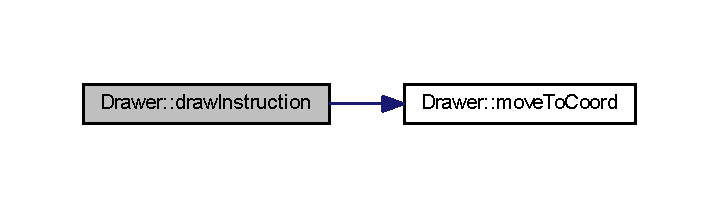
\includegraphics[width=345pt]{class_drawer_a4fb74bcad295250c519bb848dd48b0de_cgraph}
\end{center}
\end{figure}
이 함수를 호출하는 함수들에 대한 그래프입니다.\+:
\nopagebreak
\begin{figure}[H]
\begin{center}
\leavevmode
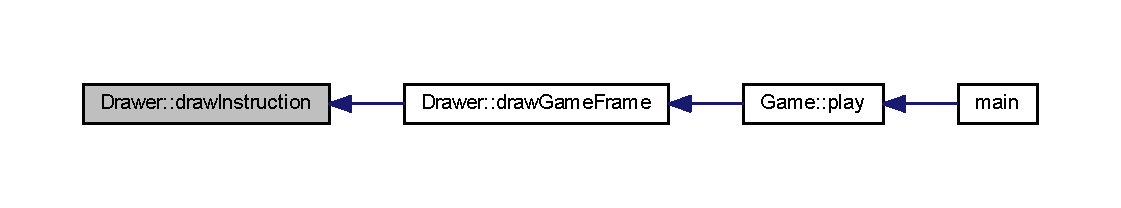
\includegraphics[width=350pt]{class_drawer_a4fb74bcad295250c519bb848dd48b0de_icgraph}
\end{center}
\end{figure}
\mbox{\Hypertarget{class_drawer_a6d8f74fa5fae96990547abb2521b5432}\label{class_drawer_a6d8f74fa5fae96990547abb2521b5432}} 
\index{Drawer@{Drawer}!draw\+Next\+Block@{draw\+Next\+Block}}
\index{draw\+Next\+Block@{draw\+Next\+Block}!Drawer@{Drawer}}
\subsubsection{\texorpdfstring{draw\+Next\+Block()}{drawNextBlock()}}
{\footnotesize\ttfamily void Drawer\+::draw\+Next\+Block (\begin{DoxyParamCaption}\item[{const \mbox{\hyperlink{class_block_handler}{Block\+Handler}} \&}]{handle }\end{DoxyParamCaption}) const\hspace{0.3cm}{\ttfamily [inline]}}



다음 블럭을 그림 



tetris\+\_\+drawer.\+h 파일의 186 번째 라인에서 정의되었습니다.


\begin{DoxyCode}
187     \{
188         \mbox{\hyperlink{class_block_ad054b4ac51df79aa910040b2a2fdf7b5}{Block::Color}} currentBlockColor = handle.\mbox{\hyperlink{class_block_handler_a7a7f96fa7c0d44f9e0fb5e52ebc9c428}{nextBlk}}->getColor();
189         SetConsoleTextAttribute(GetStdHandle(STD\_OUTPUT\_HANDLE), static\_cast<WORD>(currentBlockColor));
190         \textcolor{keywordflow}{for} (\textcolor{keyword}{auto} & cellInfo : handle.\mbox{\hyperlink{class_block_handler_a7a7f96fa7c0d44f9e0fb5e52ebc9c428}{nextBlk}}->getBlockInfo())
191         \{
192             \mbox{\hyperlink{class_drawer_ac1a96e007c07cab2e36a7c78484ee9a6}{moveToCoord}}(\mbox{\hyperlink{tetris__drawer_8h_a83cc61593b9fb64d690139400b3d760b}{nextFrameDrawCoord}}.\mbox{\hyperlink{struct_coord_a696eaa744360fc791d0e3b331c549dbe}{x}} + 4 + (cellInfo.x * 2), 
      \mbox{\hyperlink{tetris__drawer_8h_a83cc61593b9fb64d690139400b3d760b}{nextFrameDrawCoord}}.\mbox{\hyperlink{struct_coord_a214166cca70cef7dda9201689c3e81ab}{y}} + 3 + cellInfo.y);
193             std::cout << \textcolor{stringliteral}{"■"};
194         \}
195         \mbox{\hyperlink{class_drawer_ac1a96e007c07cab2e36a7c78484ee9a6}{moveToCoord}}(0, 0);   \textcolor{comment}{// 게임 플레이시 커서가 화면 구석에서 깜빡거리도록 좌표를 구석으로 이동시킴}
196     \}
\end{DoxyCode}
이 함수 내부에서 호출하는 함수들에 대한 그래프입니다.\+:
\nopagebreak
\begin{figure}[H]
\begin{center}
\leavevmode
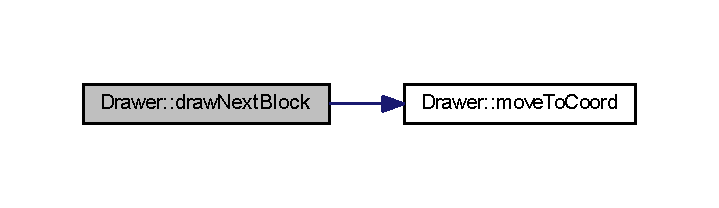
\includegraphics[width=345pt]{class_drawer_a6d8f74fa5fae96990547abb2521b5432_cgraph}
\end{center}
\end{figure}
이 함수를 호출하는 함수들에 대한 그래프입니다.\+:
\nopagebreak
\begin{figure}[H]
\begin{center}
\leavevmode
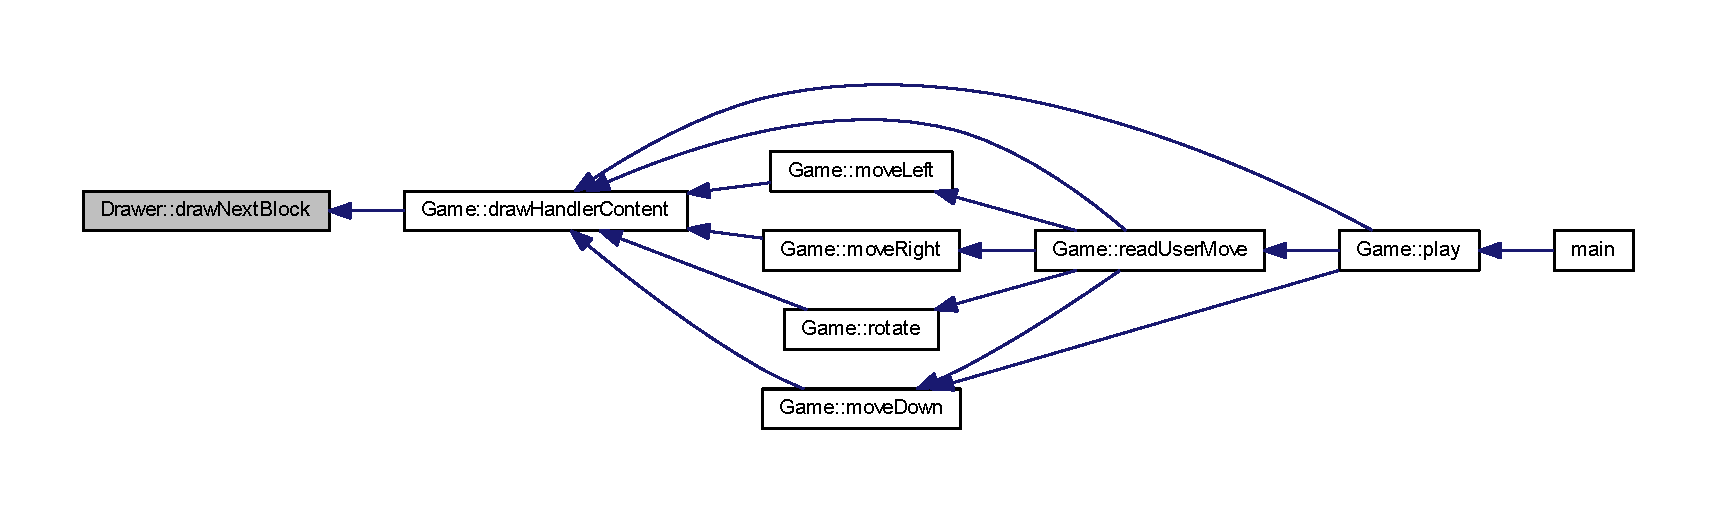
\includegraphics[width=350pt]{class_drawer_a6d8f74fa5fae96990547abb2521b5432_icgraph}
\end{center}
\end{figure}
\mbox{\Hypertarget{class_drawer_a2deae79fb268b41b72693d005cdf2178}\label{class_drawer_a2deae79fb268b41b72693d005cdf2178}} 
\index{Drawer@{Drawer}!draw\+Next\+Frame@{draw\+Next\+Frame}}
\index{draw\+Next\+Frame@{draw\+Next\+Frame}!Drawer@{Drawer}}
\subsubsection{\texorpdfstring{draw\+Next\+Frame()}{drawNextFrame()}}
{\footnotesize\ttfamily void Drawer\+::draw\+Next\+Frame (\begin{DoxyParamCaption}{ }\end{DoxyParamCaption}) const\hspace{0.3cm}{\ttfamily [inline]}, {\ttfamily [private]}}



다음 블럭을 나타낼 자리에 프레임을 그림 



tetris\+\_\+drawer.\+h 파일의 31 번째 라인에서 정의되었습니다.


\begin{DoxyCode}
32     \{
33         \mbox{\hyperlink{class_drawer_ac1a96e007c07cab2e36a7c78484ee9a6}{moveToCoord}}(\mbox{\hyperlink{tetris__drawer_8h_a83cc61593b9fb64d690139400b3d760b}{nextFrameDrawCoord}}.\mbox{\hyperlink{struct_coord_a696eaa744360fc791d0e3b331c549dbe}{x}}, 
      \mbox{\hyperlink{tetris__drawer_8h_a83cc61593b9fb64d690139400b3d760b}{nextFrameDrawCoord}}.\mbox{\hyperlink{struct_coord_a214166cca70cef7dda9201689c3e81ab}{y}});
34         std::cout << \textcolor{stringliteral}{" N  E  X  T"};
35         \mbox{\hyperlink{class_drawer_ac1a96e007c07cab2e36a7c78484ee9a6}{moveToCoord}}(\mbox{\hyperlink{tetris__drawer_8h_a83cc61593b9fb64d690139400b3d760b}{nextFrameDrawCoord}}.\mbox{\hyperlink{struct_coord_a696eaa744360fc791d0e3b331c549dbe}{x}}, 
      \mbox{\hyperlink{tetris__drawer_8h_a83cc61593b9fb64d690139400b3d760b}{nextFrameDrawCoord}}.\mbox{\hyperlink{struct_coord_a214166cca70cef7dda9201689c3e81ab}{y}} + 1);
36         \textcolor{keywordflow}{for} (\textcolor{keywordtype}{int} i = 0; i < 6; ++i)
37             std::cout << \textcolor{stringliteral}{"▩"};
38         \textcolor{keywordflow}{for} (\textcolor{keywordtype}{int} i = \mbox{\hyperlink{tetris__drawer_8h_a83cc61593b9fb64d690139400b3d760b}{nextFrameDrawCoord}}.\mbox{\hyperlink{struct_coord_a214166cca70cef7dda9201689c3e81ab}{y}} + 2; i < 
      \mbox{\hyperlink{tetris__drawer_8h_a83cc61593b9fb64d690139400b3d760b}{nextFrameDrawCoord}}.\mbox{\hyperlink{struct_coord_a214166cca70cef7dda9201689c3e81ab}{y}} + 5; ++i)
39         \{
40             \mbox{\hyperlink{class_drawer_ac1a96e007c07cab2e36a7c78484ee9a6}{moveToCoord}}(\mbox{\hyperlink{tetris__drawer_8h_a83cc61593b9fb64d690139400b3d760b}{nextFrameDrawCoord}}.\mbox{\hyperlink{struct_coord_a696eaa744360fc791d0e3b331c549dbe}{x}}, i);
41             std::cout << \textcolor{stringliteral}{"▩"};
42             \mbox{\hyperlink{class_drawer_ac1a96e007c07cab2e36a7c78484ee9a6}{moveToCoord}}(\mbox{\hyperlink{tetris__drawer_8h_a83cc61593b9fb64d690139400b3d760b}{nextFrameDrawCoord}}.\mbox{\hyperlink{struct_coord_a696eaa744360fc791d0e3b331c549dbe}{x}} + 10, i);
43             std::cout << \textcolor{stringliteral}{"▩"};
44         \}
45         \mbox{\hyperlink{class_drawer_ac1a96e007c07cab2e36a7c78484ee9a6}{moveToCoord}}(\mbox{\hyperlink{tetris__drawer_8h_a83cc61593b9fb64d690139400b3d760b}{nextFrameDrawCoord}}.\mbox{\hyperlink{struct_coord_a696eaa744360fc791d0e3b331c549dbe}{x}}, 
      \mbox{\hyperlink{tetris__drawer_8h_a83cc61593b9fb64d690139400b3d760b}{nextFrameDrawCoord}}.\mbox{\hyperlink{struct_coord_a214166cca70cef7dda9201689c3e81ab}{y}} + 5);
46         \textcolor{keywordflow}{for} (\textcolor{keywordtype}{int} i = 0; i < 6; ++i)
47             std::cout << \textcolor{stringliteral}{"▩"};
48     \}
\end{DoxyCode}
이 함수 내부에서 호출하는 함수들에 대한 그래프입니다.\+:
\nopagebreak
\begin{figure}[H]
\begin{center}
\leavevmode
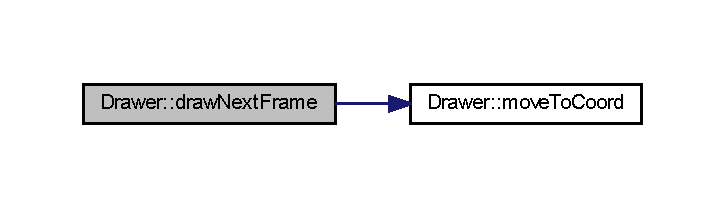
\includegraphics[width=348pt]{class_drawer_a2deae79fb268b41b72693d005cdf2178_cgraph}
\end{center}
\end{figure}
이 함수를 호출하는 함수들에 대한 그래프입니다.\+:
\nopagebreak
\begin{figure}[H]
\begin{center}
\leavevmode
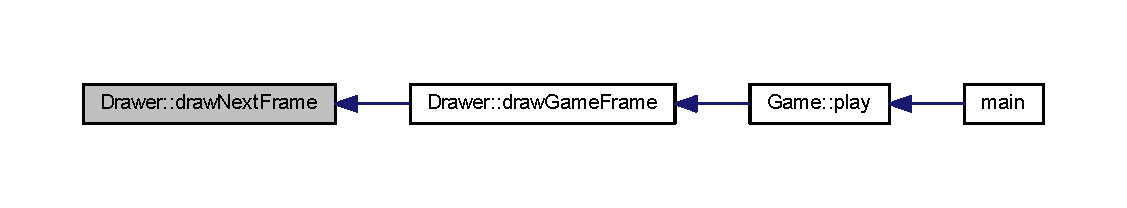
\includegraphics[width=350pt]{class_drawer_a2deae79fb268b41b72693d005cdf2178_icgraph}
\end{center}
\end{figure}
\mbox{\Hypertarget{class_drawer_ad87ca95db3cafee6f005e297e2c6d4de}\label{class_drawer_ad87ca95db3cafee6f005e297e2c6d4de}} 
\index{Drawer@{Drawer}!draw\+Title\+Screen@{draw\+Title\+Screen}}
\index{draw\+Title\+Screen@{draw\+Title\+Screen}!Drawer@{Drawer}}
\subsubsection{\texorpdfstring{draw\+Title\+Screen()}{drawTitleScreen()}}
{\footnotesize\ttfamily void Drawer\+::draw\+Title\+Screen (\begin{DoxyParamCaption}{ }\end{DoxyParamCaption}) const\hspace{0.3cm}{\ttfamily [inline]}}



타이틀 화면을 그림 



tetris\+\_\+drawer.\+h 파일의 86 번째 라인에서 정의되었습니다.


\begin{DoxyCode}
87     \{
88         system(\textcolor{stringliteral}{"cls"});
89         SetConsoleTextAttribute(GetStdHandle(STD\_OUTPUT\_HANDLE), 0x7);
90 
91         \mbox{\hyperlink{class_drawer_ac1a96e007c07cab2e36a7c78484ee9a6}{moveToCoord}}(\mbox{\hyperlink{tetris__drawer_8h_ae68c7ba7cc7e4331abf15313be5319bb}{titleScreenDrawCoord}}.\mbox{\hyperlink{struct_coord_a696eaa744360fc791d0e3b331c549dbe}{x}}, 
      \mbox{\hyperlink{tetris__drawer_8h_ae68c7ba7cc7e4331abf15313be5319bb}{titleScreenDrawCoord}}.\mbox{\hyperlink{struct_coord_a214166cca70cef7dda9201689c3e81ab}{y}}); \textcolor{comment}{// temporary}
92         std::cout << \textcolor{stringliteral}{"□□□□□□□□□□□□□□□□□□□□□□□□□□□□□□□□□□□□□\(\backslash\)n"};
93         \mbox{\hyperlink{class_drawer_ac1a96e007c07cab2e36a7c78484ee9a6}{moveToCoord}}(\mbox{\hyperlink{tetris__drawer_8h_ae68c7ba7cc7e4331abf15313be5319bb}{titleScreenDrawCoord}}.\mbox{\hyperlink{struct_coord_a696eaa744360fc791d0e3b331c549dbe}{x}}, 
      \mbox{\hyperlink{tetris__drawer_8h_ae68c7ba7cc7e4331abf15313be5319bb}{titleScreenDrawCoord}}.\mbox{\hyperlink{struct_coord_a214166cca70cef7dda9201689c3e81ab}{y}} + 1);
94         std::cout << \textcolor{stringliteral}{"□■■■■■□■■■■■□■■■■■□■■■■□□■■■■■□□■■■■□\(\backslash\)n"};
95         \mbox{\hyperlink{class_drawer_ac1a96e007c07cab2e36a7c78484ee9a6}{moveToCoord}}(\mbox{\hyperlink{tetris__drawer_8h_ae68c7ba7cc7e4331abf15313be5319bb}{titleScreenDrawCoord}}.\mbox{\hyperlink{struct_coord_a696eaa744360fc791d0e3b331c549dbe}{x}}, 
      \mbox{\hyperlink{tetris__drawer_8h_ae68c7ba7cc7e4331abf15313be5319bb}{titleScreenDrawCoord}}.\mbox{\hyperlink{struct_coord_a214166cca70cef7dda9201689c3e81ab}{y}} + 2);
96         std::cout << \textcolor{stringliteral}{"□□□■□□□■□□□□□□□■□□□■□□□■□□□■□□□■□□□□□\(\backslash\)n"};
97         \mbox{\hyperlink{class_drawer_ac1a96e007c07cab2e36a7c78484ee9a6}{moveToCoord}}(\mbox{\hyperlink{tetris__drawer_8h_ae68c7ba7cc7e4331abf15313be5319bb}{titleScreenDrawCoord}}.\mbox{\hyperlink{struct_coord_a696eaa744360fc791d0e3b331c549dbe}{x}}, 
      \mbox{\hyperlink{tetris__drawer_8h_ae68c7ba7cc7e4331abf15313be5319bb}{titleScreenDrawCoord}}.\mbox{\hyperlink{struct_coord_a214166cca70cef7dda9201689c3e81ab}{y}} + 3);
98         std::cout << \textcolor{stringliteral}{"□□□■□□□■■■■■□□□■□□□■■■■□□□□■□□□□■■■■□\(\backslash\)n"};
99         \mbox{\hyperlink{class_drawer_ac1a96e007c07cab2e36a7c78484ee9a6}{moveToCoord}}(\mbox{\hyperlink{tetris__drawer_8h_ae68c7ba7cc7e4331abf15313be5319bb}{titleScreenDrawCoord}}.\mbox{\hyperlink{struct_coord_a696eaa744360fc791d0e3b331c549dbe}{x}}, 
      \mbox{\hyperlink{tetris__drawer_8h_ae68c7ba7cc7e4331abf15313be5319bb}{titleScreenDrawCoord}}.\mbox{\hyperlink{struct_coord_a214166cca70cef7dda9201689c3e81ab}{y}} + 4);
100         std::cout << \textcolor{stringliteral}{"□□□■□□□■□□□□□□□■□□□■■■□□□□□■□□□□□□□■□\(\backslash\)n"};
101         \mbox{\hyperlink{class_drawer_ac1a96e007c07cab2e36a7c78484ee9a6}{moveToCoord}}(\mbox{\hyperlink{tetris__drawer_8h_ae68c7ba7cc7e4331abf15313be5319bb}{titleScreenDrawCoord}}.\mbox{\hyperlink{struct_coord_a696eaa744360fc791d0e3b331c549dbe}{x}}, 
      \mbox{\hyperlink{tetris__drawer_8h_ae68c7ba7cc7e4331abf15313be5319bb}{titleScreenDrawCoord}}.\mbox{\hyperlink{struct_coord_a214166cca70cef7dda9201689c3e81ab}{y}} + 5);
102         std::cout << \textcolor{stringliteral}{"□□□■□□□■■■■■□□□■□□□■□□■■□■■■■■□■■■■□□\(\backslash\)n"};
103         \mbox{\hyperlink{class_drawer_ac1a96e007c07cab2e36a7c78484ee9a6}{moveToCoord}}(\mbox{\hyperlink{tetris__drawer_8h_ae68c7ba7cc7e4331abf15313be5319bb}{titleScreenDrawCoord}}.\mbox{\hyperlink{struct_coord_a696eaa744360fc791d0e3b331c549dbe}{x}}, 
      \mbox{\hyperlink{tetris__drawer_8h_ae68c7ba7cc7e4331abf15313be5319bb}{titleScreenDrawCoord}}.\mbox{\hyperlink{struct_coord_a214166cca70cef7dda9201689c3e81ab}{y}} + 6);
104         std::cout << \textcolor{stringliteral}{"□□□□□□□□□□□□□□□□□□□□□□□□□□□□□□□□□□□□□\(\backslash\)n"};
105         \mbox{\hyperlink{class_drawer_ac1a96e007c07cab2e36a7c78484ee9a6}{moveToCoord}}(\mbox{\hyperlink{tetris__drawer_8h_ae68c7ba7cc7e4331abf15313be5319bb}{titleScreenDrawCoord}}.\mbox{\hyperlink{struct_coord_a696eaa744360fc791d0e3b331c549dbe}{x}} + 16, 
      \mbox{\hyperlink{tetris__drawer_8h_ae68c7ba7cc7e4331abf15313be5319bb}{titleScreenDrawCoord}}.\mbox{\hyperlink{struct_coord_a214166cca70cef7dda9201689c3e81ab}{y}} + 12);
106         std::cout << \textcolor{stringliteral}{"P R E S S  S P A C E  K E Y  T O  S T A R T..."};
107 
108     \}
\end{DoxyCode}
이 함수 내부에서 호출하는 함수들에 대한 그래프입니다.\+:
\nopagebreak
\begin{figure}[H]
\begin{center}
\leavevmode
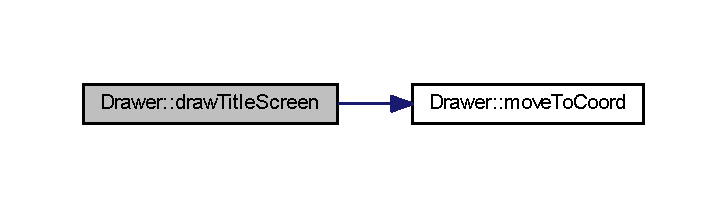
\includegraphics[width=349pt]{class_drawer_ad87ca95db3cafee6f005e297e2c6d4de_cgraph}
\end{center}
\end{figure}
이 함수를 호출하는 함수들에 대한 그래프입니다.\+:
\nopagebreak
\begin{figure}[H]
\begin{center}
\leavevmode
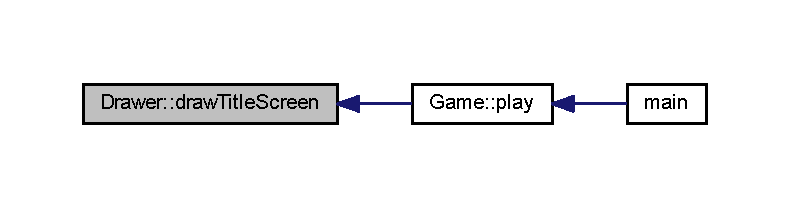
\includegraphics[width=350pt]{class_drawer_ad87ca95db3cafee6f005e297e2c6d4de_icgraph}
\end{center}
\end{figure}
\mbox{\Hypertarget{class_drawer_ad8b55aff1fbf975536ef3d995d3a4526}\label{class_drawer_ad8b55aff1fbf975536ef3d995d3a4526}} 
\index{Drawer@{Drawer}!erase\+Board@{erase\+Board}}
\index{erase\+Board@{erase\+Board}!Drawer@{Drawer}}
\subsubsection{\texorpdfstring{erase\+Board()}{eraseBoard()}}
{\footnotesize\ttfamily void Drawer\+::erase\+Board (\begin{DoxyParamCaption}\item[{const \mbox{\hyperlink{class_board}{Board}} \&}]{bd }\end{DoxyParamCaption}) const\hspace{0.3cm}{\ttfamily [inline]}}



보드를 지움 



tetris\+\_\+drawer.\+h 파일의 149 번째 라인에서 정의되었습니다.


\begin{DoxyCode}
150     \{
151         \textcolor{keyword}{const} \mbox{\hyperlink{class_board_a84bf794bc185e31e333b78bb003c4bc3}{Board::BoardType}} & status = bd.\mbox{\hyperlink{class_board_ac96b4da16e8dc266b39772f2da3fd7e2}{boardStatus}}();
152         \textcolor{keywordflow}{for} (\textcolor{keywordtype}{int} i = 0; i < 25; ++i)
153             \textcolor{keywordflow}{for} (\textcolor{keywordtype}{int} j = 0; j < 10; ++j)
154                 \textcolor{keywordflow}{if} (status[i][j].occupied == \textcolor{keyword}{true})  \textcolor{comment}{// false 시 else문을 통해 std::cout << "  "; 을 사용하면 간혹 게임이
       매우 느려짐.}
155                 \{
156                     \mbox{\hyperlink{class_drawer_ac1a96e007c07cab2e36a7c78484ee9a6}{moveToCoord}}(\mbox{\hyperlink{tetris__drawer_8h_afe5fa4d0ad1820f448b83de84142af4d}{boardDrawCoord}}.\mbox{\hyperlink{struct_coord_a696eaa744360fc791d0e3b331c549dbe}{x}} + j * 2, 
      \mbox{\hyperlink{tetris__drawer_8h_afe5fa4d0ad1820f448b83de84142af4d}{boardDrawCoord}}.\mbox{\hyperlink{struct_coord_a214166cca70cef7dda9201689c3e81ab}{y}} + i);
157                     std::cout << \textcolor{stringliteral}{"  "};
158                 \}
159     \}
\end{DoxyCode}
이 함수 내부에서 호출하는 함수들에 대한 그래프입니다.\+:
\nopagebreak
\begin{figure}[H]
\begin{center}
\leavevmode
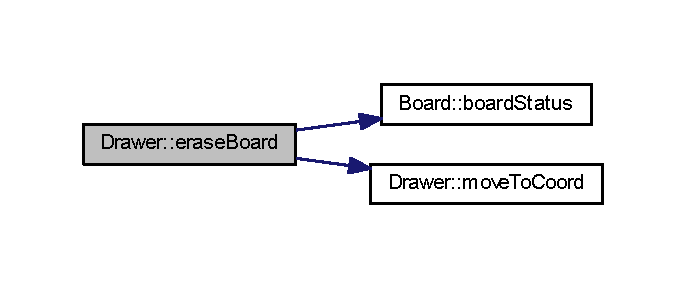
\includegraphics[width=329pt]{class_drawer_ad8b55aff1fbf975536ef3d995d3a4526_cgraph}
\end{center}
\end{figure}
이 함수를 호출하는 함수들에 대한 그래프입니다.\+:
\nopagebreak
\begin{figure}[H]
\begin{center}
\leavevmode
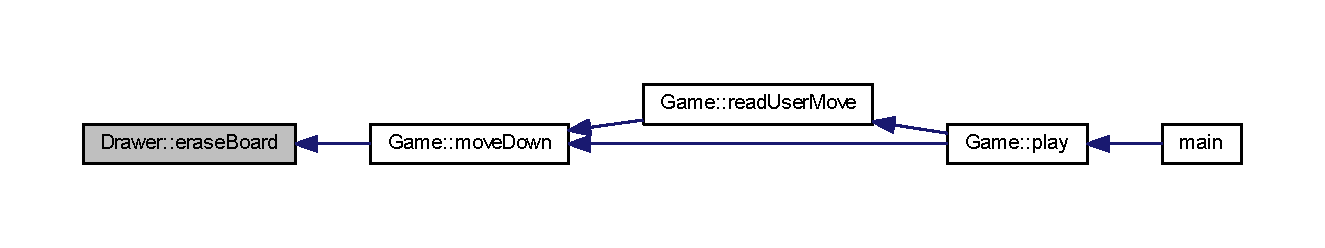
\includegraphics[width=350pt]{class_drawer_ad8b55aff1fbf975536ef3d995d3a4526_icgraph}
\end{center}
\end{figure}
\mbox{\Hypertarget{class_drawer_a513de5ba9d65771ed21918a90cd70afa}\label{class_drawer_a513de5ba9d65771ed21918a90cd70afa}} 
\index{Drawer@{Drawer}!erase\+Current\+Block@{erase\+Current\+Block}}
\index{erase\+Current\+Block@{erase\+Current\+Block}!Drawer@{Drawer}}
\subsubsection{\texorpdfstring{erase\+Current\+Block()}{eraseCurrentBlock()}}
{\footnotesize\ttfamily void Drawer\+::erase\+Current\+Block (\begin{DoxyParamCaption}\item[{const \mbox{\hyperlink{class_block_handler}{Block\+Handler}} \&}]{handle }\end{DoxyParamCaption}) const\hspace{0.3cm}{\ttfamily [inline]}}



현재 블럭을 지움 



tetris\+\_\+drawer.\+h 파일의 175 번째 라인에서 정의되었습니다.


\begin{DoxyCode}
176     \{
177         \textcolor{keywordflow}{for} (\textcolor{keyword}{auto} & cellInfo : handle.\mbox{\hyperlink{class_block_handler_ab57212ded2552ab5559d278c8538c454}{blk}}->getBlockInfo())
178         \{
179             \mbox{\hyperlink{struct_coord}{Coord}} temp = handle.\mbox{\hyperlink{class_block_handler_a11bd634fdc179446f9c6751e2394999e}{currPos}} + cellInfo;
180             \mbox{\hyperlink{class_drawer_ac1a96e007c07cab2e36a7c78484ee9a6}{moveToCoord}}(\mbox{\hyperlink{tetris__drawer_8h_afe5fa4d0ad1820f448b83de84142af4d}{boardDrawCoord}}.\mbox{\hyperlink{struct_coord_a696eaa744360fc791d0e3b331c549dbe}{x}} + temp.\mbox{\hyperlink{struct_coord_a696eaa744360fc791d0e3b331c549dbe}{x}} * 2, 
      \mbox{\hyperlink{tetris__drawer_8h_afe5fa4d0ad1820f448b83de84142af4d}{boardDrawCoord}}.\mbox{\hyperlink{struct_coord_a214166cca70cef7dda9201689c3e81ab}{y}} + temp.\mbox{\hyperlink{struct_coord_a214166cca70cef7dda9201689c3e81ab}{y}});
181             std::cout << \textcolor{stringliteral}{"  "};
182         \}
183     \}
\end{DoxyCode}
이 함수 내부에서 호출하는 함수들에 대한 그래프입니다.\+:
\nopagebreak
\begin{figure}[H]
\begin{center}
\leavevmode
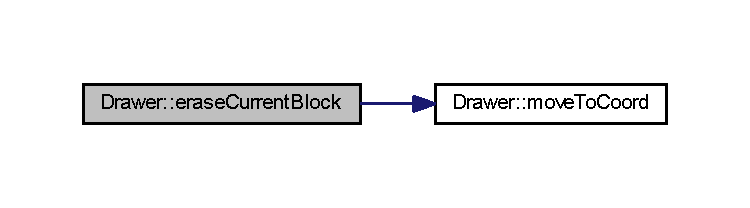
\includegraphics[width=350pt]{class_drawer_a513de5ba9d65771ed21918a90cd70afa_cgraph}
\end{center}
\end{figure}
이 함수를 호출하는 함수들에 대한 그래프입니다.\+:
\nopagebreak
\begin{figure}[H]
\begin{center}
\leavevmode
\includegraphics[width=350pt]{class_drawer_a513de5ba9d65771ed21918a90cd70afa_icgraph}
\end{center}
\end{figure}
\mbox{\Hypertarget{class_drawer_a3110e80f9256176373f0580788e69037}\label{class_drawer_a3110e80f9256176373f0580788e69037}} 
\index{Drawer@{Drawer}!erase\+Next\+Block@{erase\+Next\+Block}}
\index{erase\+Next\+Block@{erase\+Next\+Block}!Drawer@{Drawer}}
\subsubsection{\texorpdfstring{erase\+Next\+Block()}{eraseNextBlock()}}
{\footnotesize\ttfamily void Drawer\+::erase\+Next\+Block (\begin{DoxyParamCaption}\item[{const \mbox{\hyperlink{class_block_handler}{Block\+Handler}} \&}]{handle }\end{DoxyParamCaption}) const\hspace{0.3cm}{\ttfamily [inline]}}



다음 블럭을 지움 



tetris\+\_\+drawer.\+h 파일의 199 번째 라인에서 정의되었습니다.


\begin{DoxyCode}
200     \{
201         \textcolor{keywordflow}{for} (\textcolor{keyword}{auto} & cellInfo : handle.\mbox{\hyperlink{class_block_handler_a7a7f96fa7c0d44f9e0fb5e52ebc9c428}{nextBlk}}->getBlockInfo())
202         \{
203             \mbox{\hyperlink{class_drawer_ac1a96e007c07cab2e36a7c78484ee9a6}{moveToCoord}}(\mbox{\hyperlink{tetris__drawer_8h_a83cc61593b9fb64d690139400b3d760b}{nextFrameDrawCoord}}.\mbox{\hyperlink{struct_coord_a696eaa744360fc791d0e3b331c549dbe}{x}} + 4 + (cellInfo.x * 2), 
      \mbox{\hyperlink{tetris__drawer_8h_a83cc61593b9fb64d690139400b3d760b}{nextFrameDrawCoord}}.\mbox{\hyperlink{struct_coord_a214166cca70cef7dda9201689c3e81ab}{y}} + 3 + cellInfo.y);
204             std::cout << \textcolor{stringliteral}{"  "};
205         \}
206         \mbox{\hyperlink{class_drawer_ac1a96e007c07cab2e36a7c78484ee9a6}{moveToCoord}}(0, 0);
207     \}
\end{DoxyCode}
이 함수 내부에서 호출하는 함수들에 대한 그래프입니다.\+:
\nopagebreak
\begin{figure}[H]
\begin{center}
\leavevmode
\includegraphics[width=349pt]{class_drawer_a3110e80f9256176373f0580788e69037_cgraph}
\end{center}
\end{figure}
이 함수를 호출하는 함수들에 대한 그래프입니다.\+:
\nopagebreak
\begin{figure}[H]
\begin{center}
\leavevmode
\includegraphics[width=350pt]{class_drawer_a3110e80f9256176373f0580788e69037_icgraph}
\end{center}
\end{figure}
\mbox{\Hypertarget{class_drawer_ac1a96e007c07cab2e36a7c78484ee9a6}\label{class_drawer_ac1a96e007c07cab2e36a7c78484ee9a6}} 
\index{Drawer@{Drawer}!move\+To\+Coord@{move\+To\+Coord}}
\index{move\+To\+Coord@{move\+To\+Coord}!Drawer@{Drawer}}
\subsubsection{\texorpdfstring{move\+To\+Coord()}{moveToCoord()}}
{\footnotesize\ttfamily void Drawer\+::move\+To\+Coord (\begin{DoxyParamCaption}\item[{int}]{x,  }\item[{int}]{y }\end{DoxyParamCaption}) const\hspace{0.3cm}{\ttfamily [inline]}, {\ttfamily [private]}}



해당 좌표로 커서를 이동시킴 



tetris\+\_\+drawer.\+h 파일의 22 번째 라인에서 정의되었습니다.


\begin{DoxyCode}
23     \{
24         COORD cursor;
25         cursor.X = x;
26         cursor.Y = y;
27         SetConsoleCursorPosition(GetStdHandle(STD\_OUTPUT\_HANDLE), cursor);
28     \}
\end{DoxyCode}
이 함수를 호출하는 함수들에 대한 그래프입니다.\+:
\nopagebreak
\begin{figure}[H]
\begin{center}
\leavevmode
\includegraphics[width=350pt]{class_drawer_ac1a96e007c07cab2e36a7c78484ee9a6_icgraph}
\end{center}
\end{figure}


이 클래스에 대한 문서화 페이지는 다음의 파일로부터 생성되었습니다.\+:\begin{DoxyCompactItemize}
\item 
\mbox{\hyperlink{tetris__drawer_8h}{tetris\+\_\+drawer.\+h}}\end{DoxyCompactItemize}

\hypertarget{class_game}{}\section{Game 클래스 참조}
\label{class_game}\index{Game@{Game}}


\mbox{\hyperlink{class_board}{Board}}, \mbox{\hyperlink{class_block_handler}{Block\+Handler}}, Drawer를 이용하여 게임을 시작, 진행, 종료한다.  




{\ttfamily \#include $<$tetris\+\_\+game.\+h$>$}



Game에 대한 협력 다이어그램\+:
\nopagebreak
\begin{figure}[H]
\begin{center}
\leavevmode
\includegraphics[width=350pt]{class_game__coll__graph}
\end{center}
\end{figure}
\subsection*{Public 멤버 함수}
\begin{DoxyCompactItemize}
\item 
\mbox{\hyperlink{class_game_a46a5ded6c47eeab8c880ebf0d6abd0cf}{Game}} (int level)
\begin{DoxyCompactList}\small\item\em 게임의 초기 설정(블럭, 진입 위치, 난이도, 난수 시드 초기화)을 진행한다. \end{DoxyCompactList}\item 
void \mbox{\hyperlink{class_game_aa333825d0bca80e91e53c7e23f053405}{play}} ()
\begin{DoxyCompactList}\small\item\em 게임을 실행한다. \end{DoxyCompactList}\item 
void \mbox{\hyperlink{class_game_a3bd586b9c1bcd71f78bc2c2f7e2fe9e7}{move\+Left}} ()
\begin{DoxyCompactList}\small\item\em 왼쪽으로 움직일 수 있으면, 현 블럭을 옮기고 새로 그린다. \end{DoxyCompactList}\item 
void \mbox{\hyperlink{class_game_a36ee055aa2c311deea72c38f50814007}{move\+Right}} ()
\begin{DoxyCompactList}\small\item\em 오른쪽으로 움직일 수 있으면, 현 블럭을 옮기고 새로 그린다. \end{DoxyCompactList}\item 
bool \mbox{\hyperlink{class_game_af379862400da53dd8f296f0990c0953f}{move\+Down}} ()
\item 
void \mbox{\hyperlink{class_game_a8727c9c167265bff376f606d02687c6b}{rotate}} ()
\begin{DoxyCompactList}\small\item\em 현 블럭을 회전시킬 수 있으면 회전시킨다. \end{DoxyCompactList}\end{DoxyCompactItemize}
\subsection*{Private 멤버 함수}
\begin{DoxyCompactItemize}
\item 
void \mbox{\hyperlink{class_game_a00e70c3fa536c8b76e92aaca66c5ccc2}{press\+Space\+To\+Continue}} () const
\begin{DoxyCompactList}\small\item\em 사용자가 스페이스를 누를 때까지 대기한다. \end{DoxyCompactList}\item 
void \mbox{\hyperlink{class_game_aeb128045605ef167c233da9f993d407d}{read\+User\+Move}} ()
\begin{DoxyCompactList}\small\item\em 사용자의 조작을 읽어 블럭을 조작한다. \end{DoxyCompactList}\item 
void \mbox{\hyperlink{class_game_aa61075838d60bc5c850b72bc4804b7b8}{draw\+Handler\+Content}} () const
\begin{DoxyCompactList}\small\item\em 현재 블럭과 다음 블럭을 그리는 함수를 호출하는 함수. \end{DoxyCompactList}\item 
void \mbox{\hyperlink{class_game_a7ab3d17dc7bf72f0a59fbb7b17c6ce5a}{erase\+Handler\+Content}} () const
\begin{DoxyCompactList}\small\item\em 현재 블럭과 다음 블럭을 지우는 함수를 호출하는 함수. \end{DoxyCompactList}\end{DoxyCompactItemize}
\subsection*{Private 속성}
\begin{DoxyCompactItemize}
\item 
\mbox{\hyperlink{class_drawer}{Drawer}} \mbox{\hyperlink{class_game_a045e1468514c0c0d51e968364e0678ad}{drawer}}
\item 
\mbox{\hyperlink{class_board}{Board}} \mbox{\hyperlink{class_game_af5bc546b0c766ecf2f7e008f750832ed}{board}}
\item 
\mbox{\hyperlink{class_block_handler}{Block\+Handler}} \mbox{\hyperlink{class_game_ae72b7259125e83dfd258c6a132394eec}{handler}}
\item 
int \mbox{\hyperlink{class_game_a536a6390d16f05d402928bd731e06ef3}{difficulty}}
\begin{DoxyCompactList}\small\item\em 난이도를 나타내는 변수. 1 -\/ 5의 범위를 가지며, 1 높아질 수록 블럭이 100ms 빨리 내려간다. \end{DoxyCompactList}\end{DoxyCompactItemize}


\subsection{상세한 설명}
\mbox{\hyperlink{class_board}{Board}}, \mbox{\hyperlink{class_block_handler}{Block\+Handler}}, Drawer를 이용하여 게임을 시작, 진행, 종료한다. 

tetris\+\_\+game.\+h 파일의 19 번째 라인에서 정의되었습니다.



\subsection{생성자 \& 소멸자 문서화}
\mbox{\Hypertarget{class_game_a46a5ded6c47eeab8c880ebf0d6abd0cf}\label{class_game_a46a5ded6c47eeab8c880ebf0d6abd0cf}} 
\index{Game@{Game}!Game@{Game}}
\index{Game@{Game}!Game@{Game}}
\subsubsection{\texorpdfstring{Game()}{Game()}}
{\footnotesize\ttfamily Game\+::\+Game (\begin{DoxyParamCaption}\item[{int}]{level }\end{DoxyParamCaption})\hspace{0.3cm}{\ttfamily [inline]}}



게임의 초기 설정(블럭, 진입 위치, 난이도, 난수 시드 초기화)을 진행한다. 



tetris\+\_\+game.\+h 파일의 76 번째 라인에서 정의되었습니다.


\begin{DoxyCode}
76                     : \mbox{\hyperlink{class_game_af5bc546b0c766ecf2f7e008f750832ed}{board}}(), \mbox{\hyperlink{class_game_ae72b7259125e83dfd258c6a132394eec}{handler}}(\mbox{\hyperlink{class_game_af5bc546b0c766ecf2f7e008f750832ed}{board}}.\mbox{\hyperlink{class_board_a902cd3b288be772ba6b7abc6a822afea}{entryCoord}}()), 
      \mbox{\hyperlink{class_game_a536a6390d16f05d402928bd731e06ef3}{difficulty}}(level - 1)
77     \{
78         std::srand(std::time(NULL));
79     \}
\end{DoxyCode}


\subsection{멤버 함수 문서화}
\mbox{\Hypertarget{class_game_aa61075838d60bc5c850b72bc4804b7b8}\label{class_game_aa61075838d60bc5c850b72bc4804b7b8}} 
\index{Game@{Game}!draw\+Handler\+Content@{draw\+Handler\+Content}}
\index{draw\+Handler\+Content@{draw\+Handler\+Content}!Game@{Game}}
\subsubsection{\texorpdfstring{draw\+Handler\+Content()}{drawHandlerContent()}}
{\footnotesize\ttfamily void Game\+::draw\+Handler\+Content (\begin{DoxyParamCaption}{ }\end{DoxyParamCaption}) const\hspace{0.3cm}{\ttfamily [inline]}, {\ttfamily [private]}}



현재 블럭과 다음 블럭을 그리는 함수를 호출하는 함수. 



tetris\+\_\+game.\+h 파일의 60 번째 라인에서 정의되었습니다.


\begin{DoxyCode}
61     \{
62         \mbox{\hyperlink{class_game_a045e1468514c0c0d51e968364e0678ad}{drawer}}.\mbox{\hyperlink{class_drawer_acef9be5772c0a3bdbae4f01d851e60f1}{drawCurrentBlock}}(\mbox{\hyperlink{class_game_ae72b7259125e83dfd258c6a132394eec}{handler}});
63         \mbox{\hyperlink{class_game_a045e1468514c0c0d51e968364e0678ad}{drawer}}.\mbox{\hyperlink{class_drawer_a6d8f74fa5fae96990547abb2521b5432}{drawNextBlock}}(\mbox{\hyperlink{class_game_ae72b7259125e83dfd258c6a132394eec}{handler}});
64     \}
\end{DoxyCode}
이 함수 내부에서 호출하는 함수들에 대한 그래프입니다.\+:
\nopagebreak
\begin{figure}[H]
\begin{center}
\leavevmode
\includegraphics[width=350pt]{class_game_aa61075838d60bc5c850b72bc4804b7b8_cgraph}
\end{center}
\end{figure}
이 함수를 호출하는 함수들에 대한 그래프입니다.\+:
\nopagebreak
\begin{figure}[H]
\begin{center}
\leavevmode
\includegraphics[width=350pt]{class_game_aa61075838d60bc5c850b72bc4804b7b8_icgraph}
\end{center}
\end{figure}
\mbox{\Hypertarget{class_game_a7ab3d17dc7bf72f0a59fbb7b17c6ce5a}\label{class_game_a7ab3d17dc7bf72f0a59fbb7b17c6ce5a}} 
\index{Game@{Game}!erase\+Handler\+Content@{erase\+Handler\+Content}}
\index{erase\+Handler\+Content@{erase\+Handler\+Content}!Game@{Game}}
\subsubsection{\texorpdfstring{erase\+Handler\+Content()}{eraseHandlerContent()}}
{\footnotesize\ttfamily void Game\+::erase\+Handler\+Content (\begin{DoxyParamCaption}{ }\end{DoxyParamCaption}) const\hspace{0.3cm}{\ttfamily [inline]}, {\ttfamily [private]}}



현재 블럭과 다음 블럭을 지우는 함수를 호출하는 함수. 



tetris\+\_\+game.\+h 파일의 67 번째 라인에서 정의되었습니다.


\begin{DoxyCode}
68     \{
69         \mbox{\hyperlink{class_game_a045e1468514c0c0d51e968364e0678ad}{drawer}}.\mbox{\hyperlink{class_drawer_a513de5ba9d65771ed21918a90cd70afa}{eraseCurrentBlock}}(\mbox{\hyperlink{class_game_ae72b7259125e83dfd258c6a132394eec}{handler}});
70         \mbox{\hyperlink{class_game_a045e1468514c0c0d51e968364e0678ad}{drawer}}.\mbox{\hyperlink{class_drawer_a3110e80f9256176373f0580788e69037}{eraseNextBlock}}(\mbox{\hyperlink{class_game_ae72b7259125e83dfd258c6a132394eec}{handler}});
71     \}
\end{DoxyCode}
이 함수 내부에서 호출하는 함수들에 대한 그래프입니다.\+:
\nopagebreak
\begin{figure}[H]
\begin{center}
\leavevmode
\includegraphics[width=350pt]{class_game_a7ab3d17dc7bf72f0a59fbb7b17c6ce5a_cgraph}
\end{center}
\end{figure}
이 함수를 호출하는 함수들에 대한 그래프입니다.\+:
\nopagebreak
\begin{figure}[H]
\begin{center}
\leavevmode
\includegraphics[width=350pt]{class_game_a7ab3d17dc7bf72f0a59fbb7b17c6ce5a_icgraph}
\end{center}
\end{figure}
\mbox{\Hypertarget{class_game_af379862400da53dd8f296f0990c0953f}\label{class_game_af379862400da53dd8f296f0990c0953f}} 
\index{Game@{Game}!move\+Down@{move\+Down}}
\index{move\+Down@{move\+Down}!Game@{Game}}
\subsubsection{\texorpdfstring{move\+Down()}{moveDown()}}
{\footnotesize\ttfamily bool Game\+::move\+Down (\begin{DoxyParamCaption}{ }\end{DoxyParamCaption})\hspace{0.3cm}{\ttfamily [inline]}}

아래로 움직일 수 있으면, 현 블럭을 옮기고 새로 그린다. 아니라면, 보드와 현 블럭, 그리고 다음 블럭을 화면에서 지우고, 새로 고쳐 다시 그린다. \begin{DoxyReturn}{반환값}
아래로 움직였는 지 여부 
\end{DoxyReturn}


tetris\+\_\+game.\+h 파일의 139 번째 라인에서 정의되었습니다.


\begin{DoxyCode}
140     \{
141         \textcolor{keywordflow}{if} (!\mbox{\hyperlink{class_game_af5bc546b0c766ecf2f7e008f750832ed}{board}}.\mbox{\hyperlink{class_board_ad617ae22e46d1a62ed33592b20e00b44}{isDownBlocked}}(\mbox{\hyperlink{class_game_ae72b7259125e83dfd258c6a132394eec}{handler}}))
142         \{
143             \mbox{\hyperlink{class_game_a7ab3d17dc7bf72f0a59fbb7b17c6ce5a}{eraseHandlerContent}}();
144             \mbox{\hyperlink{class_game_ae72b7259125e83dfd258c6a132394eec}{handler}}.\mbox{\hyperlink{class_block_handler_a11bd634fdc179446f9c6751e2394999e}{currPos}}.\mbox{\hyperlink{struct_coord_a214166cca70cef7dda9201689c3e81ab}{y}} += 1;
145             \mbox{\hyperlink{class_game_aa61075838d60bc5c850b72bc4804b7b8}{drawHandlerContent}}();
146             \textcolor{keywordflow}{return} \textcolor{keyword}{true};
147         \}
148         \textcolor{keywordflow}{else}
149         \{
150             \mbox{\hyperlink{class_game_a045e1468514c0c0d51e968364e0678ad}{drawer}}.\mbox{\hyperlink{class_drawer_ad8b55aff1fbf975536ef3d995d3a4526}{eraseBoard}}(\mbox{\hyperlink{class_game_af5bc546b0c766ecf2f7e008f750832ed}{board}});
151             \mbox{\hyperlink{class_game_a7ab3d17dc7bf72f0a59fbb7b17c6ce5a}{eraseHandlerContent}}();
152 
153             \mbox{\hyperlink{class_game_af5bc546b0c766ecf2f7e008f750832ed}{board}}.\mbox{\hyperlink{class_board_a06e5188ef352fc5c0e3957895cef6a89}{updateBoard}}(\mbox{\hyperlink{class_game_ae72b7259125e83dfd258c6a132394eec}{handler}});  
154             \mbox{\hyperlink{class_game_ae72b7259125e83dfd258c6a132394eec}{handler}}.\mbox{\hyperlink{class_block_handler_a170a8b83b6df72530675d722a17fb8c4}{resetHandler}}();
155 
156             \textcolor{comment}{// 게임 오버라면 보드, 현 블럭, 그리고 다음 블럭을 다시 그리는 과정은 생략한다.}
157             \textcolor{keywordflow}{if} (!\mbox{\hyperlink{class_game_af5bc546b0c766ecf2f7e008f750832ed}{board}}.\mbox{\hyperlink{class_board_a538ca2c02fbccf3af07ed3c821d9a736}{isGameOver}}(\mbox{\hyperlink{class_game_ae72b7259125e83dfd258c6a132394eec}{handler}}))
158             \{
159                 \mbox{\hyperlink{class_game_a045e1468514c0c0d51e968364e0678ad}{drawer}}.\mbox{\hyperlink{class_drawer_af26df40487cb2de033887b5342d94b5a}{drawBoard}}(\mbox{\hyperlink{class_game_af5bc546b0c766ecf2f7e008f750832ed}{board}});
160                 \mbox{\hyperlink{class_game_aa61075838d60bc5c850b72bc4804b7b8}{drawHandlerContent}}();
161             \}
162             \textcolor{keywordflow}{return} \textcolor{keyword}{false};
163         \}
164     \}
\end{DoxyCode}
이 함수 내부에서 호출하는 함수들에 대한 그래프입니다.\+:
\nopagebreak
\begin{figure}[H]
\begin{center}
\leavevmode
\includegraphics[width=350pt]{class_game_af379862400da53dd8f296f0990c0953f_cgraph}
\end{center}
\end{figure}
이 함수를 호출하는 함수들에 대한 그래프입니다.\+:
\nopagebreak
\begin{figure}[H]
\begin{center}
\leavevmode
\includegraphics[width=350pt]{class_game_af379862400da53dd8f296f0990c0953f_icgraph}
\end{center}
\end{figure}
\mbox{\Hypertarget{class_game_a3bd586b9c1bcd71f78bc2c2f7e2fe9e7}\label{class_game_a3bd586b9c1bcd71f78bc2c2f7e2fe9e7}} 
\index{Game@{Game}!move\+Left@{move\+Left}}
\index{move\+Left@{move\+Left}!Game@{Game}}
\subsubsection{\texorpdfstring{move\+Left()}{moveLeft()}}
{\footnotesize\ttfamily void Game\+::move\+Left (\begin{DoxyParamCaption}{ }\end{DoxyParamCaption})\hspace{0.3cm}{\ttfamily [inline]}}



왼쪽으로 움직일 수 있으면, 현 블럭을 옮기고 새로 그린다. 



tetris\+\_\+game.\+h 파일의 112 번째 라인에서 정의되었습니다.


\begin{DoxyCode}
113     \{
114         \textcolor{keywordflow}{if} (!\mbox{\hyperlink{class_game_af5bc546b0c766ecf2f7e008f750832ed}{board}}.\mbox{\hyperlink{class_board_a5545704e21b5f7447eb9ffe014954cb3}{isLeftBlocked}}(\mbox{\hyperlink{class_game_ae72b7259125e83dfd258c6a132394eec}{handler}}))
115         \{
116             \mbox{\hyperlink{class_game_a7ab3d17dc7bf72f0a59fbb7b17c6ce5a}{eraseHandlerContent}}();
117             \mbox{\hyperlink{class_game_ae72b7259125e83dfd258c6a132394eec}{handler}}.\mbox{\hyperlink{class_block_handler_a11bd634fdc179446f9c6751e2394999e}{currPos}}.\mbox{\hyperlink{struct_coord_a696eaa744360fc791d0e3b331c549dbe}{x}} -= 1;
118             \mbox{\hyperlink{class_game_aa61075838d60bc5c850b72bc4804b7b8}{drawHandlerContent}}();
119         \}
120     \}
\end{DoxyCode}
이 함수 내부에서 호출하는 함수들에 대한 그래프입니다.\+:
\nopagebreak
\begin{figure}[H]
\begin{center}
\leavevmode
\includegraphics[width=350pt]{class_game_a3bd586b9c1bcd71f78bc2c2f7e2fe9e7_cgraph}
\end{center}
\end{figure}
이 함수를 호출하는 함수들에 대한 그래프입니다.\+:
\nopagebreak
\begin{figure}[H]
\begin{center}
\leavevmode
\includegraphics[width=350pt]{class_game_a3bd586b9c1bcd71f78bc2c2f7e2fe9e7_icgraph}
\end{center}
\end{figure}
\mbox{\Hypertarget{class_game_a36ee055aa2c311deea72c38f50814007}\label{class_game_a36ee055aa2c311deea72c38f50814007}} 
\index{Game@{Game}!move\+Right@{move\+Right}}
\index{move\+Right@{move\+Right}!Game@{Game}}
\subsubsection{\texorpdfstring{move\+Right()}{moveRight()}}
{\footnotesize\ttfamily void Game\+::move\+Right (\begin{DoxyParamCaption}{ }\end{DoxyParamCaption})\hspace{0.3cm}{\ttfamily [inline]}}



오른쪽으로 움직일 수 있으면, 현 블럭을 옮기고 새로 그린다. 



tetris\+\_\+game.\+h 파일의 123 번째 라인에서 정의되었습니다.


\begin{DoxyCode}
124     \{
125         \textcolor{keywordflow}{if} (!\mbox{\hyperlink{class_game_af5bc546b0c766ecf2f7e008f750832ed}{board}}.\mbox{\hyperlink{class_board_ad38cdb8757f58a32b5747e2b7e0be277}{isRightBlocked}}(\mbox{\hyperlink{class_game_ae72b7259125e83dfd258c6a132394eec}{handler}}))
126         \{
127             \mbox{\hyperlink{class_game_a7ab3d17dc7bf72f0a59fbb7b17c6ce5a}{eraseHandlerContent}}();
128             \mbox{\hyperlink{class_game_ae72b7259125e83dfd258c6a132394eec}{handler}}.\mbox{\hyperlink{class_block_handler_a11bd634fdc179446f9c6751e2394999e}{currPos}}.\mbox{\hyperlink{struct_coord_a696eaa744360fc791d0e3b331c549dbe}{x}} += 1;
129             \mbox{\hyperlink{class_game_aa61075838d60bc5c850b72bc4804b7b8}{drawHandlerContent}}();
130         \}
131     \}
\end{DoxyCode}
이 함수 내부에서 호출하는 함수들에 대한 그래프입니다.\+:
\nopagebreak
\begin{figure}[H]
\begin{center}
\leavevmode
\includegraphics[width=350pt]{class_game_a36ee055aa2c311deea72c38f50814007_cgraph}
\end{center}
\end{figure}
이 함수를 호출하는 함수들에 대한 그래프입니다.\+:
\nopagebreak
\begin{figure}[H]
\begin{center}
\leavevmode
\includegraphics[width=350pt]{class_game_a36ee055aa2c311deea72c38f50814007_icgraph}
\end{center}
\end{figure}
\mbox{\Hypertarget{class_game_aa333825d0bca80e91e53c7e23f053405}\label{class_game_aa333825d0bca80e91e53c7e23f053405}} 
\index{Game@{Game}!play@{play}}
\index{play@{play}!Game@{Game}}
\subsubsection{\texorpdfstring{play()}{play()}}
{\footnotesize\ttfamily void Game\+::play (\begin{DoxyParamCaption}{ }\end{DoxyParamCaption})\hspace{0.3cm}{\ttfamily [inline]}}



게임을 실행한다. 



tetris\+\_\+game.\+h 파일의 82 번째 라인에서 정의되었습니다.


\begin{DoxyCode}
83     \{
84         \mbox{\hyperlink{class_game_a045e1468514c0c0d51e968364e0678ad}{drawer}}.\mbox{\hyperlink{class_drawer_ad87ca95db3cafee6f005e297e2c6d4de}{drawTitleScreen}}(); 
85         \mbox{\hyperlink{class_game_a00e70c3fa536c8b76e92aaca66c5ccc2}{pressSpaceToContinue}}();
86         \mbox{\hyperlink{class_game_a045e1468514c0c0d51e968364e0678ad}{drawer}}.\mbox{\hyperlink{class_drawer_a9f5e10f6175710be253244d6f80ebcf7}{drawGameFrame}}();
87         \mbox{\hyperlink{class_game_a045e1468514c0c0d51e968364e0678ad}{drawer}}.\mbox{\hyperlink{class_drawer_af26df40487cb2de033887b5342d94b5a}{drawBoard}}(\mbox{\hyperlink{class_game_af5bc546b0c766ecf2f7e008f750832ed}{board}});
88         \mbox{\hyperlink{class_game_aa61075838d60bc5c850b72bc4804b7b8}{drawHandlerContent}}();
89         \textcolor{keywordtype}{int} countForAutoDown = 0;                   \textcolor{comment}{// 100ms에 1 증가하는 카운트. 블럭 자동 내림에 사용}
90         \textcolor{keywordtype}{int} countLimit = \mbox{\hyperlink{tetris__game_8h_aca9e87e8e4e22a94653954e21e81c939}{normalLevel}} - \mbox{\hyperlink{class_game_a536a6390d16f05d402928bd731e06ef3}{difficulty}};  \textcolor{comment}{// 난이도가 1에서 오를 수록 1000ms에서 100ms씩
       감소하는 카운트 제한}
91         \textcolor{keywordflow}{while} (\textcolor{keyword}{true})
92         \{
93             \textcolor{keywordflow}{if} (\mbox{\hyperlink{class_game_af5bc546b0c766ecf2f7e008f750832ed}{board}}.\mbox{\hyperlink{class_board_a538ca2c02fbccf3af07ed3c821d9a736}{isGameOver}}(\mbox{\hyperlink{class_game_ae72b7259125e83dfd258c6a132394eec}{handler}}))
94             \{
95                 Sleep(75);
96                 \mbox{\hyperlink{class_game_a045e1468514c0c0d51e968364e0678ad}{drawer}}.\mbox{\hyperlink{class_drawer_a57ec099eb46c93f20d9221a2244dd9a7}{drawGameOverScreen}}(\mbox{\hyperlink{class_game_af5bc546b0c766ecf2f7e008f750832ed}{board}});
97                 \textcolor{keywordflow}{break};
98             \}
99             
100             ++countForAutoDown;
101             \textcolor{keywordflow}{if} (countForAutoDown == countLimit) \textcolor{comment}{// 1 second}
102             \{
103                 \mbox{\hyperlink{class_game_af379862400da53dd8f296f0990c0953f}{moveDown}}();
104                 countForAutoDown = 0;
105             \}
106 
107             \mbox{\hyperlink{class_game_aeb128045605ef167c233da9f993d407d}{readUserMove}}();
108         \}
109     \}
\end{DoxyCode}
이 함수 내부에서 호출하는 함수들에 대한 그래프입니다.\+:
\nopagebreak
\begin{figure}[H]
\begin{center}
\leavevmode
\includegraphics[width=350pt]{class_game_aa333825d0bca80e91e53c7e23f053405_cgraph}
\end{center}
\end{figure}
이 함수를 호출하는 함수들에 대한 그래프입니다.\+:
\nopagebreak
\begin{figure}[H]
\begin{center}
\leavevmode
\includegraphics[width=221pt]{class_game_aa333825d0bca80e91e53c7e23f053405_icgraph}
\end{center}
\end{figure}
\mbox{\Hypertarget{class_game_a00e70c3fa536c8b76e92aaca66c5ccc2}\label{class_game_a00e70c3fa536c8b76e92aaca66c5ccc2}} 
\index{Game@{Game}!press\+Space\+To\+Continue@{press\+Space\+To\+Continue}}
\index{press\+Space\+To\+Continue@{press\+Space\+To\+Continue}!Game@{Game}}
\subsubsection{\texorpdfstring{press\+Space\+To\+Continue()}{pressSpaceToContinue()}}
{\footnotesize\ttfamily void Game\+::press\+Space\+To\+Continue (\begin{DoxyParamCaption}{ }\end{DoxyParamCaption}) const\hspace{0.3cm}{\ttfamily [inline]}, {\ttfamily [private]}}



사용자가 스페이스를 누를 때까지 대기한다. 



tetris\+\_\+game.\+h 파일의 29 번째 라인에서 정의되었습니다.


\begin{DoxyCode}
30     \{
31         \textcolor{keywordflow}{while} (\textcolor{keyword}{true})
32             \textcolor{keywordflow}{if} (GetAsyncKeyState(VK\_SPACE) & 0x8000)
33             \{
34                 Sleep(500);
35                 \textcolor{keywordflow}{break};
36             \}
37     \}
\end{DoxyCode}
이 함수를 호출하는 함수들에 대한 그래프입니다.\+:
\nopagebreak
\begin{figure}[H]
\begin{center}
\leavevmode
\includegraphics[width=350pt]{class_game_a00e70c3fa536c8b76e92aaca66c5ccc2_icgraph}
\end{center}
\end{figure}
\mbox{\Hypertarget{class_game_aeb128045605ef167c233da9f993d407d}\label{class_game_aeb128045605ef167c233da9f993d407d}} 
\index{Game@{Game}!read\+User\+Move@{read\+User\+Move}}
\index{read\+User\+Move@{read\+User\+Move}!Game@{Game}}
\subsubsection{\texorpdfstring{read\+User\+Move()}{readUserMove()}}
{\footnotesize\ttfamily void Game\+::read\+User\+Move (\begin{DoxyParamCaption}{ }\end{DoxyParamCaption})\hspace{0.3cm}{\ttfamily [inline]}, {\ttfamily [private]}}



사용자의 조작을 읽어 블럭을 조작한다. 



tetris\+\_\+game.\+h 파일의 40 번째 라인에서 정의되었습니다.


\begin{DoxyCode}
41     \{
42         \textcolor{keywordflow}{if} (GetAsyncKeyState(VK\_UP) & 0x8000)
43             \mbox{\hyperlink{class_game_a8727c9c167265bff376f606d02687c6b}{rotate}}();
44         \textcolor{keywordflow}{if} (GetAsyncKeyState(VK\_DOWN) & 0x8000)
45             \mbox{\hyperlink{class_game_af379862400da53dd8f296f0990c0953f}{moveDown}}();
46         \textcolor{keywordflow}{if} (GetAsyncKeyState(VK\_LEFT) & 0x8000)
47             \mbox{\hyperlink{class_game_a3bd586b9c1bcd71f78bc2c2f7e2fe9e7}{moveLeft}}();
48         \textcolor{keywordflow}{if} (GetAsyncKeyState(VK\_RIGHT) & 0x8000)
49             \mbox{\hyperlink{class_game_a36ee055aa2c311deea72c38f50814007}{moveRight}}();
50         \textcolor{keywordflow}{if} (GetAsyncKeyState(VK\_SPACE) & 0x8000)
51         \{
52             \textcolor{keywordflow}{while} (\mbox{\hyperlink{class_game_af379862400da53dd8f296f0990c0953f}{moveDown}}())
53                 \textcolor{keywordflow}{continue};
54             \mbox{\hyperlink{class_game_aa61075838d60bc5c850b72bc4804b7b8}{drawHandlerContent}}();
55         \}
56         Sleep(100);
57     \}
\end{DoxyCode}
이 함수 내부에서 호출하는 함수들에 대한 그래프입니다.\+:
\nopagebreak
\begin{figure}[H]
\begin{center}
\leavevmode
\includegraphics[width=350pt]{class_game_aeb128045605ef167c233da9f993d407d_cgraph}
\end{center}
\end{figure}
이 함수를 호출하는 함수들에 대한 그래프입니다.\+:
\nopagebreak
\begin{figure}[H]
\begin{center}
\leavevmode
\includegraphics[width=350pt]{class_game_aeb128045605ef167c233da9f993d407d_icgraph}
\end{center}
\end{figure}
\mbox{\Hypertarget{class_game_a8727c9c167265bff376f606d02687c6b}\label{class_game_a8727c9c167265bff376f606d02687c6b}} 
\index{Game@{Game}!rotate@{rotate}}
\index{rotate@{rotate}!Game@{Game}}
\subsubsection{\texorpdfstring{rotate()}{rotate()}}
{\footnotesize\ttfamily void Game\+::rotate (\begin{DoxyParamCaption}{ }\end{DoxyParamCaption})\hspace{0.3cm}{\ttfamily [inline]}}



현 블럭을 회전시킬 수 있으면 회전시킨다. 



tetris\+\_\+game.\+h 파일의 167 번째 라인에서 정의되었습니다.


\begin{DoxyCode}
168     \{
169         \textcolor{keywordflow}{if} (!\mbox{\hyperlink{class_game_af5bc546b0c766ecf2f7e008f750832ed}{board}}.\mbox{\hyperlink{class_board_a4b84310dd1ac3a08a3180361508a43e3}{isNotRotatable}}(\mbox{\hyperlink{class_game_ae72b7259125e83dfd258c6a132394eec}{handler}}))
170         \{
171             \mbox{\hyperlink{class_game_a7ab3d17dc7bf72f0a59fbb7b17c6ce5a}{eraseHandlerContent}}();
172             \mbox{\hyperlink{class_game_ae72b7259125e83dfd258c6a132394eec}{handler}}.\mbox{\hyperlink{class_block_handler_ab57212ded2552ab5559d278c8538c454}{blk}}->rotate();
173             \mbox{\hyperlink{class_game_aa61075838d60bc5c850b72bc4804b7b8}{drawHandlerContent}}();
174         \}
175     \}
\end{DoxyCode}
이 함수 내부에서 호출하는 함수들에 대한 그래프입니다.\+:
\nopagebreak
\begin{figure}[H]
\begin{center}
\leavevmode
\includegraphics[width=350pt]{class_game_a8727c9c167265bff376f606d02687c6b_cgraph}
\end{center}
\end{figure}
이 함수를 호출하는 함수들에 대한 그래프입니다.\+:
\nopagebreak
\begin{figure}[H]
\begin{center}
\leavevmode
\includegraphics[width=350pt]{class_game_a8727c9c167265bff376f606d02687c6b_icgraph}
\end{center}
\end{figure}


\subsection{멤버 데이터 문서화}
\mbox{\Hypertarget{class_game_af5bc546b0c766ecf2f7e008f750832ed}\label{class_game_af5bc546b0c766ecf2f7e008f750832ed}} 
\index{Game@{Game}!board@{board}}
\index{board@{board}!Game@{Game}}
\subsubsection{\texorpdfstring{board}{board}}
{\footnotesize\ttfamily \mbox{\hyperlink{class_board}{Board}} Game\+::board\hspace{0.3cm}{\ttfamily [private]}}



tetris\+\_\+game.\+h 파일의 24 번째 라인에서 정의되었습니다.

\mbox{\Hypertarget{class_game_a536a6390d16f05d402928bd731e06ef3}\label{class_game_a536a6390d16f05d402928bd731e06ef3}} 
\index{Game@{Game}!difficulty@{difficulty}}
\index{difficulty@{difficulty}!Game@{Game}}
\subsubsection{\texorpdfstring{difficulty}{difficulty}}
{\footnotesize\ttfamily int Game\+::difficulty\hspace{0.3cm}{\ttfamily [private]}}



난이도를 나타내는 변수. 1 -\/ 5의 범위를 가지며, 1 높아질 수록 블럭이 100ms 빨리 내려간다. 



tetris\+\_\+game.\+h 파일의 26 번째 라인에서 정의되었습니다.

\mbox{\Hypertarget{class_game_a045e1468514c0c0d51e968364e0678ad}\label{class_game_a045e1468514c0c0d51e968364e0678ad}} 
\index{Game@{Game}!drawer@{drawer}}
\index{drawer@{drawer}!Game@{Game}}
\subsubsection{\texorpdfstring{drawer}{drawer}}
{\footnotesize\ttfamily \mbox{\hyperlink{class_drawer}{Drawer}} Game\+::drawer\hspace{0.3cm}{\ttfamily [private]}}



tetris\+\_\+game.\+h 파일의 23 번째 라인에서 정의되었습니다.

\mbox{\Hypertarget{class_game_ae72b7259125e83dfd258c6a132394eec}\label{class_game_ae72b7259125e83dfd258c6a132394eec}} 
\index{Game@{Game}!handler@{handler}}
\index{handler@{handler}!Game@{Game}}
\subsubsection{\texorpdfstring{handler}{handler}}
{\footnotesize\ttfamily \mbox{\hyperlink{class_block_handler}{Block\+Handler}} Game\+::handler\hspace{0.3cm}{\ttfamily [private]}}



tetris\+\_\+game.\+h 파일의 25 번째 라인에서 정의되었습니다.



이 클래스에 대한 문서화 페이지는 다음의 파일로부터 생성되었습니다.\+:\begin{DoxyCompactItemize}
\item 
\mbox{\hyperlink{tetris__game_8h}{tetris\+\_\+game.\+h}}\end{DoxyCompactItemize}

\hypertarget{class_i}{}\section{I 클래스 참조}
\label{class_i}\index{I@{I}}


\mbox{\hyperlink{class_i}{I}} 모양 블럭  




{\ttfamily \#include $<$tetris\+\_\+block.\+h$>$}



I에 대한 상속 다이어그램 \+: 
\nopagebreak
\begin{figure}[H]
\begin{center}
\leavevmode
\includegraphics[width=185pt]{class_i__inherit__graph}
\end{center}
\end{figure}


I에 대한 협력 다이어그램\+:
\nopagebreak
\begin{figure}[H]
\begin{center}
\leavevmode
\includegraphics[width=185pt]{class_i__coll__graph}
\end{center}
\end{figure}
\subsection*{Public 타입}
\begin{DoxyCompactItemize}
\item 
enum \mbox{\hyperlink{class_block_a33a96023993478ad4b52426188454765}{Mode}} \{ \newline
\mbox{\hyperlink{class_block_a33a96023993478ad4b52426188454765a4529e89ca1c08cc5f81181e355719fad}{U\+P\+S\+I\+DE}}, 
\mbox{\hyperlink{class_block_a33a96023993478ad4b52426188454765a9c855bf91465e7da98901d7900740919}{L\+E\+F\+T\+S\+I\+DE}}, 
\mbox{\hyperlink{class_block_a33a96023993478ad4b52426188454765a73fd4ad0ff8642235ec8549f9290d13b}{D\+O\+W\+N\+S\+I\+DE}}, 
\mbox{\hyperlink{class_block_a33a96023993478ad4b52426188454765a005424e665ea0b83edfaf9ddb3ab85a1}{R\+I\+G\+H\+T\+S\+I\+DE}}, 
\newline
\mbox{\hyperlink{class_block_a33a96023993478ad4b52426188454765a76628d7877667ccb2f6e549b89466a4a}{V\+E\+R\+T\+I\+C\+AL}}, 
\mbox{\hyperlink{class_block_a33a96023993478ad4b52426188454765a883bda1b4a0cb6d25d8b3c3465f0cfef}{H\+O\+R\+I\+Z\+O\+N\+T\+AL}}
 \}
\begin{DoxyCompactList}\small\item\em 블럭들의 회전 상태를 나타내는 enum type \end{DoxyCompactList}\item 
enum \mbox{\hyperlink{class_block_ad054b4ac51df79aa910040b2a2fdf7b5}{Color}} \{ \newline
\mbox{\hyperlink{class_block_ad054b4ac51df79aa910040b2a2fdf7b5acd0cdefe1b7ef4fc0c9b47a765ae00ca}{B\+L\+A\+CK}}, 
\mbox{\hyperlink{class_block_ad054b4ac51df79aa910040b2a2fdf7b5a770f3d9456df6e3e286c001f0ffc835f}{B\+L\+UE}}, 
\mbox{\hyperlink{class_block_ad054b4ac51df79aa910040b2a2fdf7b5ac7f4e27e7581d2456d7db6b52514800d}{G\+R\+E\+EN}}, 
\mbox{\hyperlink{class_block_ad054b4ac51df79aa910040b2a2fdf7b5aa6acf45f9e85e879c50413b30769006a}{T\+U\+RQ}}, 
\newline
\mbox{\hyperlink{class_block_ad054b4ac51df79aa910040b2a2fdf7b5ac3d067e89682bb3d91db42beb7c68062}{R\+ED}}, 
\mbox{\hyperlink{class_block_ad054b4ac51df79aa910040b2a2fdf7b5adf5ec5d70a53f3465e863f43e9118588}{P\+U\+R\+P\+LE}}, 
\mbox{\hyperlink{class_block_ad054b4ac51df79aa910040b2a2fdf7b5a7ae21b7c7ed4cd37d641a5119d0b3939}{Y\+E\+L\+L\+OW}}, 
\mbox{\hyperlink{class_block_ad054b4ac51df79aa910040b2a2fdf7b5a37ab7320f3ca5662b117fb110adb1011}{W\+H\+I\+TE}}, 
\newline
\mbox{\hyperlink{class_block_ad054b4ac51df79aa910040b2a2fdf7b5a1158efe2e537f0b96f9ea590f22ab821}{G\+R\+AY}}, 
\mbox{\hyperlink{class_block_ad054b4ac51df79aa910040b2a2fdf7b5aad861330fd0e7f87dbfbe9ceb49785b3}{P\+A\+L\+E\+B\+L\+UE}}, 
\mbox{\hyperlink{class_block_ad054b4ac51df79aa910040b2a2fdf7b5ad7542730815e74f4f9a9df7fec33d3b5}{P\+A\+L\+E\+G\+R\+E\+EN}}, 
\mbox{\hyperlink{class_block_ad054b4ac51df79aa910040b2a2fdf7b5acbe4a64f95830b01b5be63b91544d452}{P\+A\+L\+E\+T\+U\+RQ}}, 
\newline
\mbox{\hyperlink{class_block_ad054b4ac51df79aa910040b2a2fdf7b5a9a1a56423a8c5b1b51fb11d184ced4cd}{P\+A\+L\+E\+R\+ED}}, 
\mbox{\hyperlink{class_block_ad054b4ac51df79aa910040b2a2fdf7b5ae78300d2e1540cc8a58c4018a2b902a6}{P\+A\+L\+E\+P\+U\+R\+P\+LE}}, 
\mbox{\hyperlink{class_block_ad054b4ac51df79aa910040b2a2fdf7b5ac09cccdee282b3a0c1331e2892042bea}{P\+A\+L\+E\+Y\+E\+L\+L\+OW}}, 
\mbox{\hyperlink{class_block_ad054b4ac51df79aa910040b2a2fdf7b5af606ae67cebcef81e9ee80f1411d4247}{B\+R\+I\+G\+H\+T\+W\+H\+I\+TE}}
 \}
\begin{DoxyCompactList}\small\item\em 블럭들이 가질 수 있는 색상을 나타내는 enum type \end{DoxyCompactList}\item 
typedef std\+::array$<$ \mbox{\hyperlink{struct_coord}{Coord}}, 4 $>$ \mbox{\hyperlink{class_block_aca5d951639f113e2ebd7856209d6b9ab}{Block\+Shape}}
\begin{DoxyCompactList}\small\item\em 블럭의 모양 정보를 좌표의 배열로 나타냄. \end{DoxyCompactList}\end{DoxyCompactItemize}
\subsection*{Public 멤버 함수}
\begin{DoxyCompactItemize}
\item 
\mbox{\hyperlink{class_i_ae21899806c8e3ea9c22b8ca5f6d1b949}{I}} ()
\item 
void \mbox{\hyperlink{class_i_a5ee89d0f1ddc27429dfd0c83edf86ad5}{rotate}} () override
\begin{DoxyCompactList}\small\item\em 회전 상태를 다음 회전 상태로 변경 (한 번에 90도 회전) \end{DoxyCompactList}\item 
const \mbox{\hyperlink{class_block_ad054b4ac51df79aa910040b2a2fdf7b5}{Color}} \mbox{\hyperlink{class_i_afa15b62959b0207778d0db1763aff784}{get\+Color}} () override
\begin{DoxyCompactList}\small\item\em 블럭의 색상 정보를 리턴 \end{DoxyCompactList}\item 
const \mbox{\hyperlink{class_block_aca5d951639f113e2ebd7856209d6b9ab}{Block\+Shape}} \& \mbox{\hyperlink{class_i_a21f835547d478a560c6616d8ca81e966}{get\+Block\+Info}} () override
\begin{DoxyCompactList}\small\item\em 블럭의 현재 회전 상태에 따른 모양 정보 리턴 \end{DoxyCompactList}\item 
const \mbox{\hyperlink{class_block_aca5d951639f113e2ebd7856209d6b9ab}{Block\+Shape}} \& \mbox{\hyperlink{class_i_ae5a6c09baa0575ff54446278a32a900a}{get\+Next\+Block\+Info}} () override
\begin{DoxyCompactList}\small\item\em 회전을 1번 더 했을 경우의 모양 정보 리턴 \end{DoxyCompactList}\end{DoxyCompactItemize}
\subsection*{Private 속성}
\begin{DoxyCompactItemize}
\item 
\mbox{\hyperlink{class_block_a33a96023993478ad4b52426188454765}{Mode}} \mbox{\hyperlink{class_i_a97884fed99bc779803178b5c3f4bc02d}{mode}}
\begin{DoxyCompactList}\small\item\em 회전 상태(가로, 세로) \end{DoxyCompactList}\end{DoxyCompactItemize}
\subsection*{정적 Private 속성}
\begin{DoxyCompactItemize}
\item 
static const \mbox{\hyperlink{class_block_ad054b4ac51df79aa910040b2a2fdf7b5}{Color}} \mbox{\hyperlink{class_i_a526ab692f8757d9d3ff3da5ca231b8a0}{color}} = \mbox{\hyperlink{class_block_ad054b4ac51df79aa910040b2a2fdf7b5ac3d067e89682bb3d91db42beb7c68062}{R\+ED}}
\begin{DoxyCompactList}\small\item\em 블럭의 색상 \end{DoxyCompactList}\item 
static const \mbox{\hyperlink{class_block_aca5d951639f113e2ebd7856209d6b9ab}{Block\+Shape}} \mbox{\hyperlink{class_i_a78fdc2abb810f708c2595846c74ad1ca}{block\+Info\+Vertical}} \{ \{\{0, 0\}, \{0, 1 \}, \{0, 2 \}, \{0, 3\}\} \}
\begin{DoxyCompactList}\small\item\em 세로로 회전되어있을 경우의 모양 정보 \end{DoxyCompactList}\item 
static const \mbox{\hyperlink{class_block_aca5d951639f113e2ebd7856209d6b9ab}{Block\+Shape}} \mbox{\hyperlink{class_i_af8e5eabbd3a5e1fef9066d3a6fa44adc}{block\+Info\+Horizontal}} \{ \{\{-\/1, 0\}, \{0, 0\}, \{1, 0\}, \{2, 0\}\} \}
\begin{DoxyCompactList}\small\item\em 가로로 회전되어있을 경우의 모양 정보 \end{DoxyCompactList}\end{DoxyCompactItemize}


\subsection{상세한 설명}
\mbox{\hyperlink{class_i}{I}} 모양 블럭 

tetris\+\_\+block.\+h 파일의 48 번째 라인에서 정의되었습니다.



\subsection{멤버 타입정의 문서화}
\mbox{\Hypertarget{class_block_aca5d951639f113e2ebd7856209d6b9ab}\label{class_block_aca5d951639f113e2ebd7856209d6b9ab}} 
\index{I@{I}!Block\+Shape@{Block\+Shape}}
\index{Block\+Shape@{Block\+Shape}!I@{I}}
\subsubsection{\texorpdfstring{Block\+Shape}{BlockShape}}
{\footnotesize\ttfamily typedef std\+::array$<$\mbox{\hyperlink{struct_coord}{Coord}}, 4$>$ \mbox{\hyperlink{class_block_aca5d951639f113e2ebd7856209d6b9ab}{Block\+::\+Block\+Shape}}\hspace{0.3cm}{\ttfamily [inherited]}}



블럭의 모양 정보를 좌표의 배열로 나타냄. 



tetris\+\_\+block.\+h 파일의 36 번째 라인에서 정의되었습니다.



\subsection{멤버 열거형 문서화}
\mbox{\Hypertarget{class_block_ad054b4ac51df79aa910040b2a2fdf7b5}\label{class_block_ad054b4ac51df79aa910040b2a2fdf7b5}} 
\index{I@{I}!Color@{Color}}
\index{Color@{Color}!I@{I}}
\subsubsection{\texorpdfstring{Color}{Color}}
{\footnotesize\ttfamily enum \mbox{\hyperlink{class_block_ad054b4ac51df79aa910040b2a2fdf7b5}{Block\+::\+Color}}\hspace{0.3cm}{\ttfamily [inherited]}}



블럭들이 가질 수 있는 색상을 나타내는 enum type 

\begin{DoxyEnumFields}{열거형 멤버}
\raisebox{\heightof{T}}[0pt][0pt]{\index{B\+L\+A\+CK@{B\+L\+A\+CK}!I@{I}}\index{I@{I}!B\+L\+A\+CK@{B\+L\+A\+CK}}}\mbox{\Hypertarget{class_block_ad054b4ac51df79aa910040b2a2fdf7b5acd0cdefe1b7ef4fc0c9b47a765ae00ca}\label{class_block_ad054b4ac51df79aa910040b2a2fdf7b5acd0cdefe1b7ef4fc0c9b47a765ae00ca}} 
B\+L\+A\+CK&\\
\hline

\raisebox{\heightof{T}}[0pt][0pt]{\index{B\+L\+UE@{B\+L\+UE}!I@{I}}\index{I@{I}!B\+L\+UE@{B\+L\+UE}}}\mbox{\Hypertarget{class_block_ad054b4ac51df79aa910040b2a2fdf7b5a770f3d9456df6e3e286c001f0ffc835f}\label{class_block_ad054b4ac51df79aa910040b2a2fdf7b5a770f3d9456df6e3e286c001f0ffc835f}} 
B\+L\+UE&\\
\hline

\raisebox{\heightof{T}}[0pt][0pt]{\index{G\+R\+E\+EN@{G\+R\+E\+EN}!I@{I}}\index{I@{I}!G\+R\+E\+EN@{G\+R\+E\+EN}}}\mbox{\Hypertarget{class_block_ad054b4ac51df79aa910040b2a2fdf7b5ac7f4e27e7581d2456d7db6b52514800d}\label{class_block_ad054b4ac51df79aa910040b2a2fdf7b5ac7f4e27e7581d2456d7db6b52514800d}} 
G\+R\+E\+EN&\\
\hline

\raisebox{\heightof{T}}[0pt][0pt]{\index{T\+U\+RQ@{T\+U\+RQ}!I@{I}}\index{I@{I}!T\+U\+RQ@{T\+U\+RQ}}}\mbox{\Hypertarget{class_block_ad054b4ac51df79aa910040b2a2fdf7b5aa6acf45f9e85e879c50413b30769006a}\label{class_block_ad054b4ac51df79aa910040b2a2fdf7b5aa6acf45f9e85e879c50413b30769006a}} 
T\+U\+RQ&\\
\hline

\raisebox{\heightof{T}}[0pt][0pt]{\index{R\+ED@{R\+ED}!I@{I}}\index{I@{I}!R\+ED@{R\+ED}}}\mbox{\Hypertarget{class_block_ad054b4ac51df79aa910040b2a2fdf7b5ac3d067e89682bb3d91db42beb7c68062}\label{class_block_ad054b4ac51df79aa910040b2a2fdf7b5ac3d067e89682bb3d91db42beb7c68062}} 
R\+ED&\\
\hline

\raisebox{\heightof{T}}[0pt][0pt]{\index{P\+U\+R\+P\+LE@{P\+U\+R\+P\+LE}!I@{I}}\index{I@{I}!P\+U\+R\+P\+LE@{P\+U\+R\+P\+LE}}}\mbox{\Hypertarget{class_block_ad054b4ac51df79aa910040b2a2fdf7b5adf5ec5d70a53f3465e863f43e9118588}\label{class_block_ad054b4ac51df79aa910040b2a2fdf7b5adf5ec5d70a53f3465e863f43e9118588}} 
P\+U\+R\+P\+LE&\\
\hline

\raisebox{\heightof{T}}[0pt][0pt]{\index{Y\+E\+L\+L\+OW@{Y\+E\+L\+L\+OW}!I@{I}}\index{I@{I}!Y\+E\+L\+L\+OW@{Y\+E\+L\+L\+OW}}}\mbox{\Hypertarget{class_block_ad054b4ac51df79aa910040b2a2fdf7b5a7ae21b7c7ed4cd37d641a5119d0b3939}\label{class_block_ad054b4ac51df79aa910040b2a2fdf7b5a7ae21b7c7ed4cd37d641a5119d0b3939}} 
Y\+E\+L\+L\+OW&\\
\hline

\raisebox{\heightof{T}}[0pt][0pt]{\index{W\+H\+I\+TE@{W\+H\+I\+TE}!I@{I}}\index{I@{I}!W\+H\+I\+TE@{W\+H\+I\+TE}}}\mbox{\Hypertarget{class_block_ad054b4ac51df79aa910040b2a2fdf7b5a37ab7320f3ca5662b117fb110adb1011}\label{class_block_ad054b4ac51df79aa910040b2a2fdf7b5a37ab7320f3ca5662b117fb110adb1011}} 
W\+H\+I\+TE&\\
\hline

\raisebox{\heightof{T}}[0pt][0pt]{\index{G\+R\+AY@{G\+R\+AY}!I@{I}}\index{I@{I}!G\+R\+AY@{G\+R\+AY}}}\mbox{\Hypertarget{class_block_ad054b4ac51df79aa910040b2a2fdf7b5a1158efe2e537f0b96f9ea590f22ab821}\label{class_block_ad054b4ac51df79aa910040b2a2fdf7b5a1158efe2e537f0b96f9ea590f22ab821}} 
G\+R\+AY&\\
\hline

\raisebox{\heightof{T}}[0pt][0pt]{\index{P\+A\+L\+E\+B\+L\+UE@{P\+A\+L\+E\+B\+L\+UE}!I@{I}}\index{I@{I}!P\+A\+L\+E\+B\+L\+UE@{P\+A\+L\+E\+B\+L\+UE}}}\mbox{\Hypertarget{class_block_ad054b4ac51df79aa910040b2a2fdf7b5aad861330fd0e7f87dbfbe9ceb49785b3}\label{class_block_ad054b4ac51df79aa910040b2a2fdf7b5aad861330fd0e7f87dbfbe9ceb49785b3}} 
P\+A\+L\+E\+B\+L\+UE&\\
\hline

\raisebox{\heightof{T}}[0pt][0pt]{\index{P\+A\+L\+E\+G\+R\+E\+EN@{P\+A\+L\+E\+G\+R\+E\+EN}!I@{I}}\index{I@{I}!P\+A\+L\+E\+G\+R\+E\+EN@{P\+A\+L\+E\+G\+R\+E\+EN}}}\mbox{\Hypertarget{class_block_ad054b4ac51df79aa910040b2a2fdf7b5ad7542730815e74f4f9a9df7fec33d3b5}\label{class_block_ad054b4ac51df79aa910040b2a2fdf7b5ad7542730815e74f4f9a9df7fec33d3b5}} 
P\+A\+L\+E\+G\+R\+E\+EN&\\
\hline

\raisebox{\heightof{T}}[0pt][0pt]{\index{P\+A\+L\+E\+T\+U\+RQ@{P\+A\+L\+E\+T\+U\+RQ}!I@{I}}\index{I@{I}!P\+A\+L\+E\+T\+U\+RQ@{P\+A\+L\+E\+T\+U\+RQ}}}\mbox{\Hypertarget{class_block_ad054b4ac51df79aa910040b2a2fdf7b5acbe4a64f95830b01b5be63b91544d452}\label{class_block_ad054b4ac51df79aa910040b2a2fdf7b5acbe4a64f95830b01b5be63b91544d452}} 
P\+A\+L\+E\+T\+U\+RQ&\\
\hline

\raisebox{\heightof{T}}[0pt][0pt]{\index{P\+A\+L\+E\+R\+ED@{P\+A\+L\+E\+R\+ED}!I@{I}}\index{I@{I}!P\+A\+L\+E\+R\+ED@{P\+A\+L\+E\+R\+ED}}}\mbox{\Hypertarget{class_block_ad054b4ac51df79aa910040b2a2fdf7b5a9a1a56423a8c5b1b51fb11d184ced4cd}\label{class_block_ad054b4ac51df79aa910040b2a2fdf7b5a9a1a56423a8c5b1b51fb11d184ced4cd}} 
P\+A\+L\+E\+R\+ED&\\
\hline

\raisebox{\heightof{T}}[0pt][0pt]{\index{P\+A\+L\+E\+P\+U\+R\+P\+LE@{P\+A\+L\+E\+P\+U\+R\+P\+LE}!I@{I}}\index{I@{I}!P\+A\+L\+E\+P\+U\+R\+P\+LE@{P\+A\+L\+E\+P\+U\+R\+P\+LE}}}\mbox{\Hypertarget{class_block_ad054b4ac51df79aa910040b2a2fdf7b5ae78300d2e1540cc8a58c4018a2b902a6}\label{class_block_ad054b4ac51df79aa910040b2a2fdf7b5ae78300d2e1540cc8a58c4018a2b902a6}} 
P\+A\+L\+E\+P\+U\+R\+P\+LE&\\
\hline

\raisebox{\heightof{T}}[0pt][0pt]{\index{P\+A\+L\+E\+Y\+E\+L\+L\+OW@{P\+A\+L\+E\+Y\+E\+L\+L\+OW}!I@{I}}\index{I@{I}!P\+A\+L\+E\+Y\+E\+L\+L\+OW@{P\+A\+L\+E\+Y\+E\+L\+L\+OW}}}\mbox{\Hypertarget{class_block_ad054b4ac51df79aa910040b2a2fdf7b5ac09cccdee282b3a0c1331e2892042bea}\label{class_block_ad054b4ac51df79aa910040b2a2fdf7b5ac09cccdee282b3a0c1331e2892042bea}} 
P\+A\+L\+E\+Y\+E\+L\+L\+OW&\\
\hline

\raisebox{\heightof{T}}[0pt][0pt]{\index{B\+R\+I\+G\+H\+T\+W\+H\+I\+TE@{B\+R\+I\+G\+H\+T\+W\+H\+I\+TE}!I@{I}}\index{I@{I}!B\+R\+I\+G\+H\+T\+W\+H\+I\+TE@{B\+R\+I\+G\+H\+T\+W\+H\+I\+TE}}}\mbox{\Hypertarget{class_block_ad054b4ac51df79aa910040b2a2fdf7b5af606ae67cebcef81e9ee80f1411d4247}\label{class_block_ad054b4ac51df79aa910040b2a2fdf7b5af606ae67cebcef81e9ee80f1411d4247}} 
B\+R\+I\+G\+H\+T\+W\+H\+I\+TE&\\
\hline

\end{DoxyEnumFields}


tetris\+\_\+block.\+h 파일의 31 번째 라인에서 정의되었습니다.


\begin{DoxyCode}
32     \{
33         \mbox{\hyperlink{class_block_ad054b4ac51df79aa910040b2a2fdf7b5acd0cdefe1b7ef4fc0c9b47a765ae00ca}{BLACK}}, \mbox{\hyperlink{class_block_ad054b4ac51df79aa910040b2a2fdf7b5a770f3d9456df6e3e286c001f0ffc835f}{BLUE}}, \mbox{\hyperlink{class_block_ad054b4ac51df79aa910040b2a2fdf7b5ac7f4e27e7581d2456d7db6b52514800d}{GREEN}}, \mbox{\hyperlink{class_block_ad054b4ac51df79aa910040b2a2fdf7b5aa6acf45f9e85e879c50413b30769006a}{TURQ}}, \mbox{\hyperlink{class_block_ad054b4ac51df79aa910040b2a2fdf7b5ac3d067e89682bb3d91db42beb7c68062}{RED}}, \mbox{\hyperlink{class_block_ad054b4ac51df79aa910040b2a2fdf7b5adf5ec5d70a53f3465e863f43e9118588}{PURPLE}}, \mbox{\hyperlink{class_block_ad054b4ac51df79aa910040b2a2fdf7b5a7ae21b7c7ed4cd37d641a5119d0b3939}{YELLOW}}, 
      \mbox{\hyperlink{class_block_ad054b4ac51df79aa910040b2a2fdf7b5a37ab7320f3ca5662b117fb110adb1011}{WHITE}}, \mbox{\hyperlink{class_block_ad054b4ac51df79aa910040b2a2fdf7b5a1158efe2e537f0b96f9ea590f22ab821}{GRAY}},
34         \mbox{\hyperlink{class_block_ad054b4ac51df79aa910040b2a2fdf7b5aad861330fd0e7f87dbfbe9ceb49785b3}{PALEBLUE}}, \mbox{\hyperlink{class_block_ad054b4ac51df79aa910040b2a2fdf7b5ad7542730815e74f4f9a9df7fec33d3b5}{PALEGREEN}}, \mbox{\hyperlink{class_block_ad054b4ac51df79aa910040b2a2fdf7b5acbe4a64f95830b01b5be63b91544d452}{PALETURQ}}, \mbox{\hyperlink{class_block_ad054b4ac51df79aa910040b2a2fdf7b5a9a1a56423a8c5b1b51fb11d184ced4cd}{PALERED}}, 
      \mbox{\hyperlink{class_block_ad054b4ac51df79aa910040b2a2fdf7b5ae78300d2e1540cc8a58c4018a2b902a6}{PALEPURPLE}}, \mbox{\hyperlink{class_block_ad054b4ac51df79aa910040b2a2fdf7b5ac09cccdee282b3a0c1331e2892042bea}{PALEYELLOW}}, \mbox{\hyperlink{class_block_ad054b4ac51df79aa910040b2a2fdf7b5af606ae67cebcef81e9ee80f1411d4247}{BRIGHTWHITE}}
35     \};
\end{DoxyCode}
\mbox{\Hypertarget{class_block_a33a96023993478ad4b52426188454765}\label{class_block_a33a96023993478ad4b52426188454765}} 
\index{I@{I}!Mode@{Mode}}
\index{Mode@{Mode}!I@{I}}
\subsubsection{\texorpdfstring{Mode}{Mode}}
{\footnotesize\ttfamily enum \mbox{\hyperlink{class_block_a33a96023993478ad4b52426188454765}{Block\+::\+Mode}}\hspace{0.3cm}{\ttfamily [inherited]}}



블럭들의 회전 상태를 나타내는 enum type 

\begin{DoxyEnumFields}{열거형 멤버}
\raisebox{\heightof{T}}[0pt][0pt]{\index{U\+P\+S\+I\+DE@{U\+P\+S\+I\+DE}!I@{I}}\index{I@{I}!U\+P\+S\+I\+DE@{U\+P\+S\+I\+DE}}}\mbox{\Hypertarget{class_block_a33a96023993478ad4b52426188454765a4529e89ca1c08cc5f81181e355719fad}\label{class_block_a33a96023993478ad4b52426188454765a4529e89ca1c08cc5f81181e355719fad}} 
U\+P\+S\+I\+DE&\\
\hline

\raisebox{\heightof{T}}[0pt][0pt]{\index{L\+E\+F\+T\+S\+I\+DE@{L\+E\+F\+T\+S\+I\+DE}!I@{I}}\index{I@{I}!L\+E\+F\+T\+S\+I\+DE@{L\+E\+F\+T\+S\+I\+DE}}}\mbox{\Hypertarget{class_block_a33a96023993478ad4b52426188454765a9c855bf91465e7da98901d7900740919}\label{class_block_a33a96023993478ad4b52426188454765a9c855bf91465e7da98901d7900740919}} 
L\+E\+F\+T\+S\+I\+DE&\\
\hline

\raisebox{\heightof{T}}[0pt][0pt]{\index{D\+O\+W\+N\+S\+I\+DE@{D\+O\+W\+N\+S\+I\+DE}!I@{I}}\index{I@{I}!D\+O\+W\+N\+S\+I\+DE@{D\+O\+W\+N\+S\+I\+DE}}}\mbox{\Hypertarget{class_block_a33a96023993478ad4b52426188454765a73fd4ad0ff8642235ec8549f9290d13b}\label{class_block_a33a96023993478ad4b52426188454765a73fd4ad0ff8642235ec8549f9290d13b}} 
D\+O\+W\+N\+S\+I\+DE&\\
\hline

\raisebox{\heightof{T}}[0pt][0pt]{\index{R\+I\+G\+H\+T\+S\+I\+DE@{R\+I\+G\+H\+T\+S\+I\+DE}!I@{I}}\index{I@{I}!R\+I\+G\+H\+T\+S\+I\+DE@{R\+I\+G\+H\+T\+S\+I\+DE}}}\mbox{\Hypertarget{class_block_a33a96023993478ad4b52426188454765a005424e665ea0b83edfaf9ddb3ab85a1}\label{class_block_a33a96023993478ad4b52426188454765a005424e665ea0b83edfaf9ddb3ab85a1}} 
R\+I\+G\+H\+T\+S\+I\+DE&\\
\hline

\raisebox{\heightof{T}}[0pt][0pt]{\index{V\+E\+R\+T\+I\+C\+AL@{V\+E\+R\+T\+I\+C\+AL}!I@{I}}\index{I@{I}!V\+E\+R\+T\+I\+C\+AL@{V\+E\+R\+T\+I\+C\+AL}}}\mbox{\Hypertarget{class_block_a33a96023993478ad4b52426188454765a76628d7877667ccb2f6e549b89466a4a}\label{class_block_a33a96023993478ad4b52426188454765a76628d7877667ccb2f6e549b89466a4a}} 
V\+E\+R\+T\+I\+C\+AL&\\
\hline

\raisebox{\heightof{T}}[0pt][0pt]{\index{H\+O\+R\+I\+Z\+O\+N\+T\+AL@{H\+O\+R\+I\+Z\+O\+N\+T\+AL}!I@{I}}\index{I@{I}!H\+O\+R\+I\+Z\+O\+N\+T\+AL@{H\+O\+R\+I\+Z\+O\+N\+T\+AL}}}\mbox{\Hypertarget{class_block_a33a96023993478ad4b52426188454765a883bda1b4a0cb6d25d8b3c3465f0cfef}\label{class_block_a33a96023993478ad4b52426188454765a883bda1b4a0cb6d25d8b3c3465f0cfef}} 
H\+O\+R\+I\+Z\+O\+N\+T\+AL&\\
\hline

\end{DoxyEnumFields}


tetris\+\_\+block.\+h 파일의 28 번째 라인에서 정의되었습니다.


\begin{DoxyCode}
28 \{ \mbox{\hyperlink{class_block_a33a96023993478ad4b52426188454765a4529e89ca1c08cc5f81181e355719fad}{UPSIDE}}, \mbox{\hyperlink{class_block_a33a96023993478ad4b52426188454765a9c855bf91465e7da98901d7900740919}{LEFTSIDE}}, \mbox{\hyperlink{class_block_a33a96023993478ad4b52426188454765a73fd4ad0ff8642235ec8549f9290d13b}{DOWNSIDE}}, \mbox{\hyperlink{class_block_a33a96023993478ad4b52426188454765a005424e665ea0b83edfaf9ddb3ab85a1}{RIGHTSIDE}}, \mbox{\hyperlink{class_block_a33a96023993478ad4b52426188454765a76628d7877667ccb2f6e549b89466a4a}{VERTICAL}}, 
      \mbox{\hyperlink{class_block_a33a96023993478ad4b52426188454765a883bda1b4a0cb6d25d8b3c3465f0cfef}{HORIZONTAL}} \}; 
\end{DoxyCode}


\subsection{생성자 \& 소멸자 문서화}
\mbox{\Hypertarget{class_i_ae21899806c8e3ea9c22b8ca5f6d1b949}\label{class_i_ae21899806c8e3ea9c22b8ca5f6d1b949}} 
\index{I@{I}!I@{I}}
\index{I@{I}!I@{I}}
\subsubsection{\texorpdfstring{I()}{I()}}
{\footnotesize\ttfamily I\+::I (\begin{DoxyParamCaption}{ }\end{DoxyParamCaption})\hspace{0.3cm}{\ttfamily [inline]}}



tetris\+\_\+block.\+h 파일의 58 번째 라인에서 정의되었습니다.


\begin{DoxyCode}
58 : \mbox{\hyperlink{class_i_a97884fed99bc779803178b5c3f4bc02d}{mode}}(\mbox{\hyperlink{class_block_a33a96023993478ad4b52426188454765a883bda1b4a0cb6d25d8b3c3465f0cfef}{HORIZONTAL}}) \{\}
\end{DoxyCode}


\subsection{멤버 함수 문서화}
\mbox{\Hypertarget{class_i_a21f835547d478a560c6616d8ca81e966}\label{class_i_a21f835547d478a560c6616d8ca81e966}} 
\index{I@{I}!get\+Block\+Info@{get\+Block\+Info}}
\index{get\+Block\+Info@{get\+Block\+Info}!I@{I}}
\subsubsection{\texorpdfstring{get\+Block\+Info()}{getBlockInfo()}}
{\footnotesize\ttfamily const \mbox{\hyperlink{class_block_aca5d951639f113e2ebd7856209d6b9ab}{Block\+Shape}}\& I\+::get\+Block\+Info (\begin{DoxyParamCaption}{ }\end{DoxyParamCaption})\hspace{0.3cm}{\ttfamily [inline]}, {\ttfamily [override]}, {\ttfamily [virtual]}}



블럭의 현재 회전 상태에 따른 모양 정보 리턴 



\mbox{\hyperlink{class_block_a2cdc0af223d621add42ac6c37fede329}{Block}}를 구현.



tetris\+\_\+block.\+h 파일의 70 번째 라인에서 정의되었습니다.


\begin{DoxyCode}
71     \{
72         \textcolor{keywordflow}{switch} (\mbox{\hyperlink{class_i_a97884fed99bc779803178b5c3f4bc02d}{mode}})
73         \{
74         \textcolor{keywordflow}{case} \mbox{\hyperlink{class_block_a33a96023993478ad4b52426188454765a76628d7877667ccb2f6e549b89466a4a}{VERTICAL}}:
75             \textcolor{keywordflow}{return} \mbox{\hyperlink{class_i_a78fdc2abb810f708c2595846c74ad1ca}{blockInfoVertical}};
76         \textcolor{keywordflow}{case} \mbox{\hyperlink{class_block_a33a96023993478ad4b52426188454765a883bda1b4a0cb6d25d8b3c3465f0cfef}{HORIZONTAL}}:
77             \textcolor{keywordflow}{return} \mbox{\hyperlink{class_i_af8e5eabbd3a5e1fef9066d3a6fa44adc}{blockInfoHorizontal}};
78         \}
79     \}
\end{DoxyCode}
\mbox{\Hypertarget{class_i_afa15b62959b0207778d0db1763aff784}\label{class_i_afa15b62959b0207778d0db1763aff784}} 
\index{I@{I}!get\+Color@{get\+Color}}
\index{get\+Color@{get\+Color}!I@{I}}
\subsubsection{\texorpdfstring{get\+Color()}{getColor()}}
{\footnotesize\ttfamily const \mbox{\hyperlink{class_block_ad054b4ac51df79aa910040b2a2fdf7b5}{Color}} I\+::get\+Color (\begin{DoxyParamCaption}{ }\end{DoxyParamCaption})\hspace{0.3cm}{\ttfamily [inline]}, {\ttfamily [override]}, {\ttfamily [virtual]}}



블럭의 색상 정보를 리턴 



\mbox{\hyperlink{class_block_af10efef648f21dc708e42e149cd6fbcf}{Block}}를 구현.



tetris\+\_\+block.\+h 파일의 65 번째 라인에서 정의되었습니다.


\begin{DoxyCode}
66     \{
67         \textcolor{keywordflow}{return} \mbox{\hyperlink{class_i_a526ab692f8757d9d3ff3da5ca231b8a0}{color}};
68     \}
\end{DoxyCode}
\mbox{\Hypertarget{class_i_ae5a6c09baa0575ff54446278a32a900a}\label{class_i_ae5a6c09baa0575ff54446278a32a900a}} 
\index{I@{I}!get\+Next\+Block\+Info@{get\+Next\+Block\+Info}}
\index{get\+Next\+Block\+Info@{get\+Next\+Block\+Info}!I@{I}}
\subsubsection{\texorpdfstring{get\+Next\+Block\+Info()}{getNextBlockInfo()}}
{\footnotesize\ttfamily const \mbox{\hyperlink{class_block_aca5d951639f113e2ebd7856209d6b9ab}{Block\+Shape}}\& I\+::get\+Next\+Block\+Info (\begin{DoxyParamCaption}{ }\end{DoxyParamCaption})\hspace{0.3cm}{\ttfamily [inline]}, {\ttfamily [override]}, {\ttfamily [virtual]}}



회전을 1번 더 했을 경우의 모양 정보 리턴 



\mbox{\hyperlink{class_block_a654da164e0493be9de6f2f2334bc73e8}{Block}}를 구현.



tetris\+\_\+block.\+h 파일의 81 번째 라인에서 정의되었습니다.


\begin{DoxyCode}
82     \{
83         \textcolor{keywordflow}{switch} (\mbox{\hyperlink{class_i_a97884fed99bc779803178b5c3f4bc02d}{mode}})
84         \{
85         \textcolor{keywordflow}{case} \mbox{\hyperlink{class_block_a33a96023993478ad4b52426188454765a76628d7877667ccb2f6e549b89466a4a}{VERTICAL}}:
86             \textcolor{keywordflow}{return} \mbox{\hyperlink{class_i_af8e5eabbd3a5e1fef9066d3a6fa44adc}{blockInfoHorizontal}};
87         \textcolor{keywordflow}{case} \mbox{\hyperlink{class_block_a33a96023993478ad4b52426188454765a883bda1b4a0cb6d25d8b3c3465f0cfef}{HORIZONTAL}}:
88             \textcolor{keywordflow}{return} \mbox{\hyperlink{class_i_a78fdc2abb810f708c2595846c74ad1ca}{blockInfoVertical}};
89         \}
90     \}
\end{DoxyCode}
\mbox{\Hypertarget{class_i_a5ee89d0f1ddc27429dfd0c83edf86ad5}\label{class_i_a5ee89d0f1ddc27429dfd0c83edf86ad5}} 
\index{I@{I}!rotate@{rotate}}
\index{rotate@{rotate}!I@{I}}
\subsubsection{\texorpdfstring{rotate()}{rotate()}}
{\footnotesize\ttfamily void I\+::rotate (\begin{DoxyParamCaption}{ }\end{DoxyParamCaption})\hspace{0.3cm}{\ttfamily [inline]}, {\ttfamily [override]}, {\ttfamily [virtual]}}



회전 상태를 다음 회전 상태로 변경 (한 번에 90도 회전) 



\mbox{\hyperlink{class_block_af1499ad7e48fb750581b471d0d5bb0e0}{Block}}를 구현.



tetris\+\_\+block.\+h 파일의 60 번째 라인에서 정의되었습니다.


\begin{DoxyCode}
61     \{
62         \mbox{\hyperlink{class_i_a97884fed99bc779803178b5c3f4bc02d}{mode}} == \mbox{\hyperlink{class_block_a33a96023993478ad4b52426188454765a76628d7877667ccb2f6e549b89466a4a}{VERTICAL}} ? \mbox{\hyperlink{class_i_a97884fed99bc779803178b5c3f4bc02d}{mode}} = \mbox{\hyperlink{class_block_a33a96023993478ad4b52426188454765a883bda1b4a0cb6d25d8b3c3465f0cfef}{HORIZONTAL}} : \mbox{\hyperlink{class_i_a97884fed99bc779803178b5c3f4bc02d}{mode}} = 
      \mbox{\hyperlink{class_block_a33a96023993478ad4b52426188454765a76628d7877667ccb2f6e549b89466a4a}{VERTICAL}};
63     \}
\end{DoxyCode}


\subsection{멤버 데이터 문서화}
\mbox{\Hypertarget{class_i_af8e5eabbd3a5e1fef9066d3a6fa44adc}\label{class_i_af8e5eabbd3a5e1fef9066d3a6fa44adc}} 
\index{I@{I}!block\+Info\+Horizontal@{block\+Info\+Horizontal}}
\index{block\+Info\+Horizontal@{block\+Info\+Horizontal}!I@{I}}
\subsubsection{\texorpdfstring{block\+Info\+Horizontal}{blockInfoHorizontal}}
{\footnotesize\ttfamily const \mbox{\hyperlink{class_block_aca5d951639f113e2ebd7856209d6b9ab}{Block\+::\+Block\+Shape}} I\+::block\+Info\+Horizontal \{ \{\{-\/1, 0\}, \{0, 0\}, \{1, 0\}, \{2, 0\}\} \}\hspace{0.3cm}{\ttfamily [static]}, {\ttfamily [private]}}



가로로 회전되어있을 경우의 모양 정보 



tetris\+\_\+block.\+h 파일의 54 번째 라인에서 정의되었습니다.

\mbox{\Hypertarget{class_i_a78fdc2abb810f708c2595846c74ad1ca}\label{class_i_a78fdc2abb810f708c2595846c74ad1ca}} 
\index{I@{I}!block\+Info\+Vertical@{block\+Info\+Vertical}}
\index{block\+Info\+Vertical@{block\+Info\+Vertical}!I@{I}}
\subsubsection{\texorpdfstring{block\+Info\+Vertical}{blockInfoVertical}}
{\footnotesize\ttfamily const \mbox{\hyperlink{class_block_aca5d951639f113e2ebd7856209d6b9ab}{Block\+::\+Block\+Shape}} I\+::block\+Info\+Vertical \{ \{\{0, 0\}, \{0, 1 \}, \{0, 2 \}, \{0, 3\}\} \}\hspace{0.3cm}{\ttfamily [static]}, {\ttfamily [private]}}



세로로 회전되어있을 경우의 모양 정보 



tetris\+\_\+block.\+h 파일의 53 번째 라인에서 정의되었습니다.

\mbox{\Hypertarget{class_i_a526ab692f8757d9d3ff3da5ca231b8a0}\label{class_i_a526ab692f8757d9d3ff3da5ca231b8a0}} 
\index{I@{I}!color@{color}}
\index{color@{color}!I@{I}}
\subsubsection{\texorpdfstring{color}{color}}
{\footnotesize\ttfamily const \mbox{\hyperlink{class_block_ad054b4ac51df79aa910040b2a2fdf7b5}{Block\+::\+Color}} I\+::color = \mbox{\hyperlink{class_block_ad054b4ac51df79aa910040b2a2fdf7b5ac3d067e89682bb3d91db42beb7c68062}{R\+ED}}\hspace{0.3cm}{\ttfamily [static]}, {\ttfamily [private]}}



블럭의 색상 



tetris\+\_\+block.\+h 파일의 52 번째 라인에서 정의되었습니다.

\mbox{\Hypertarget{class_i_a97884fed99bc779803178b5c3f4bc02d}\label{class_i_a97884fed99bc779803178b5c3f4bc02d}} 
\index{I@{I}!mode@{mode}}
\index{mode@{mode}!I@{I}}
\subsubsection{\texorpdfstring{mode}{mode}}
{\footnotesize\ttfamily \mbox{\hyperlink{class_block_a33a96023993478ad4b52426188454765}{Mode}} I\+::mode\hspace{0.3cm}{\ttfamily [private]}}



회전 상태(가로, 세로) 



tetris\+\_\+block.\+h 파일의 51 번째 라인에서 정의되었습니다.



이 클래스에 대한 문서화 페이지는 다음의 파일로부터 생성되었습니다.\+:\begin{DoxyCompactItemize}
\item 
\mbox{\hyperlink{tetris__block_8h}{tetris\+\_\+block.\+h}}\end{DoxyCompactItemize}

\hypertarget{class_j}{}\section{J 클래스 참조}
\label{class_j}\index{J@{J}}


\mbox{\hyperlink{class_j}{J}} 모양 블럭  




{\ttfamily \#include $<$tetris\+\_\+block.\+h$>$}



J에 대한 상속 다이어그램 \+: 
\nopagebreak
\begin{figure}[H]
\begin{center}
\leavevmode
\includegraphics[width=185pt]{class_j__inherit__graph}
\end{center}
\end{figure}


J에 대한 협력 다이어그램\+:
\nopagebreak
\begin{figure}[H]
\begin{center}
\leavevmode
\includegraphics[width=185pt]{class_j__coll__graph}
\end{center}
\end{figure}
\subsection*{Public 타입}
\begin{DoxyCompactItemize}
\item 
enum \mbox{\hyperlink{class_block_a33a96023993478ad4b52426188454765}{Mode}} \{ \newline
\mbox{\hyperlink{class_block_a33a96023993478ad4b52426188454765a4529e89ca1c08cc5f81181e355719fad}{U\+P\+S\+I\+DE}}, 
\mbox{\hyperlink{class_block_a33a96023993478ad4b52426188454765a9c855bf91465e7da98901d7900740919}{L\+E\+F\+T\+S\+I\+DE}}, 
\mbox{\hyperlink{class_block_a33a96023993478ad4b52426188454765a73fd4ad0ff8642235ec8549f9290d13b}{D\+O\+W\+N\+S\+I\+DE}}, 
\mbox{\hyperlink{class_block_a33a96023993478ad4b52426188454765a005424e665ea0b83edfaf9ddb3ab85a1}{R\+I\+G\+H\+T\+S\+I\+DE}}, 
\newline
\mbox{\hyperlink{class_block_a33a96023993478ad4b52426188454765a76628d7877667ccb2f6e549b89466a4a}{V\+E\+R\+T\+I\+C\+AL}}, 
\mbox{\hyperlink{class_block_a33a96023993478ad4b52426188454765a883bda1b4a0cb6d25d8b3c3465f0cfef}{H\+O\+R\+I\+Z\+O\+N\+T\+AL}}
 \}
\begin{DoxyCompactList}\small\item\em 블럭들의 회전 상태를 나타내는 enum type \end{DoxyCompactList}\item 
enum \mbox{\hyperlink{class_block_ad054b4ac51df79aa910040b2a2fdf7b5}{Color}} \{ \newline
\mbox{\hyperlink{class_block_ad054b4ac51df79aa910040b2a2fdf7b5acd0cdefe1b7ef4fc0c9b47a765ae00ca}{B\+L\+A\+CK}}, 
\mbox{\hyperlink{class_block_ad054b4ac51df79aa910040b2a2fdf7b5a770f3d9456df6e3e286c001f0ffc835f}{B\+L\+UE}}, 
\mbox{\hyperlink{class_block_ad054b4ac51df79aa910040b2a2fdf7b5ac7f4e27e7581d2456d7db6b52514800d}{G\+R\+E\+EN}}, 
\mbox{\hyperlink{class_block_ad054b4ac51df79aa910040b2a2fdf7b5aa6acf45f9e85e879c50413b30769006a}{T\+U\+RQ}}, 
\newline
\mbox{\hyperlink{class_block_ad054b4ac51df79aa910040b2a2fdf7b5ac3d067e89682bb3d91db42beb7c68062}{R\+ED}}, 
\mbox{\hyperlink{class_block_ad054b4ac51df79aa910040b2a2fdf7b5adf5ec5d70a53f3465e863f43e9118588}{P\+U\+R\+P\+LE}}, 
\mbox{\hyperlink{class_block_ad054b4ac51df79aa910040b2a2fdf7b5a7ae21b7c7ed4cd37d641a5119d0b3939}{Y\+E\+L\+L\+OW}}, 
\mbox{\hyperlink{class_block_ad054b4ac51df79aa910040b2a2fdf7b5a37ab7320f3ca5662b117fb110adb1011}{W\+H\+I\+TE}}, 
\newline
\mbox{\hyperlink{class_block_ad054b4ac51df79aa910040b2a2fdf7b5a1158efe2e537f0b96f9ea590f22ab821}{G\+R\+AY}}, 
\mbox{\hyperlink{class_block_ad054b4ac51df79aa910040b2a2fdf7b5aad861330fd0e7f87dbfbe9ceb49785b3}{P\+A\+L\+E\+B\+L\+UE}}, 
\mbox{\hyperlink{class_block_ad054b4ac51df79aa910040b2a2fdf7b5ad7542730815e74f4f9a9df7fec33d3b5}{P\+A\+L\+E\+G\+R\+E\+EN}}, 
\mbox{\hyperlink{class_block_ad054b4ac51df79aa910040b2a2fdf7b5acbe4a64f95830b01b5be63b91544d452}{P\+A\+L\+E\+T\+U\+RQ}}, 
\newline
\mbox{\hyperlink{class_block_ad054b4ac51df79aa910040b2a2fdf7b5a9a1a56423a8c5b1b51fb11d184ced4cd}{P\+A\+L\+E\+R\+ED}}, 
\mbox{\hyperlink{class_block_ad054b4ac51df79aa910040b2a2fdf7b5ae78300d2e1540cc8a58c4018a2b902a6}{P\+A\+L\+E\+P\+U\+R\+P\+LE}}, 
\mbox{\hyperlink{class_block_ad054b4ac51df79aa910040b2a2fdf7b5ac09cccdee282b3a0c1331e2892042bea}{P\+A\+L\+E\+Y\+E\+L\+L\+OW}}, 
\mbox{\hyperlink{class_block_ad054b4ac51df79aa910040b2a2fdf7b5af606ae67cebcef81e9ee80f1411d4247}{B\+R\+I\+G\+H\+T\+W\+H\+I\+TE}}
 \}
\begin{DoxyCompactList}\small\item\em 블럭들이 가질 수 있는 색상을 나타내는 enum type \end{DoxyCompactList}\item 
typedef std\+::array$<$ \mbox{\hyperlink{struct_coord}{Coord}}, 4 $>$ \mbox{\hyperlink{class_block_aca5d951639f113e2ebd7856209d6b9ab}{Block\+Shape}}
\begin{DoxyCompactList}\small\item\em 블럭의 모양 정보를 좌표의 배열로 나타냄. \end{DoxyCompactList}\end{DoxyCompactItemize}
\subsection*{Public 멤버 함수}
\begin{DoxyCompactItemize}
\item 
\mbox{\hyperlink{class_j_ae3dc8b3467ed8bfd545c3b72bc9c3e70}{J}} ()
\item 
void \mbox{\hyperlink{class_j_a79f9fdd2b9542a95d3d2f82381b1cb62}{rotate}} () override
\begin{DoxyCompactList}\small\item\em 회전 상태를 다음 회전 상태로 변경 (한 번에 90도 회전) \end{DoxyCompactList}\item 
const \mbox{\hyperlink{class_block_ad054b4ac51df79aa910040b2a2fdf7b5}{Color}} \mbox{\hyperlink{class_j_a9055b5b54907c2fe1b9973cd74fc9c3e}{get\+Color}} () override
\begin{DoxyCompactList}\small\item\em 블럭의 색상 정보를 리턴 \end{DoxyCompactList}\item 
const \mbox{\hyperlink{class_block_aca5d951639f113e2ebd7856209d6b9ab}{Block\+Shape}} \& \mbox{\hyperlink{class_j_a2ef290578088ff6206767f6624748284}{get\+Block\+Info}} () override
\begin{DoxyCompactList}\small\item\em 블럭의 현재 회전 상태에 따른 모양 정보 리턴 \end{DoxyCompactList}\item 
const \mbox{\hyperlink{class_block_aca5d951639f113e2ebd7856209d6b9ab}{Block\+Shape}} \& \mbox{\hyperlink{class_j_aeeaf9ab45ccf61d0e7435e3d1bf04300}{get\+Next\+Block\+Info}} () override
\begin{DoxyCompactList}\small\item\em 회전을 1번 더 했을 경우의 모양 정보 리턴 \end{DoxyCompactList}\end{DoxyCompactItemize}
\subsection*{Private 속성}
\begin{DoxyCompactItemize}
\item 
\mbox{\hyperlink{class_block_a33a96023993478ad4b52426188454765}{Mode}} \mbox{\hyperlink{class_j_a84f29c2144ce2c8ca0d369060589f0f4}{mode}}
\begin{DoxyCompactList}\small\item\em 회전 상태(가로, 세로) \end{DoxyCompactList}\end{DoxyCompactItemize}
\subsection*{정적 Private 속성}
\begin{DoxyCompactItemize}
\item 
static const \mbox{\hyperlink{class_block_ad054b4ac51df79aa910040b2a2fdf7b5}{Color}} \mbox{\hyperlink{class_j_adf3d9ba6faa25890b274cba9eabf02e5}{color}} = \mbox{\hyperlink{class_block_ad054b4ac51df79aa910040b2a2fdf7b5a7ae21b7c7ed4cd37d641a5119d0b3939}{Y\+E\+L\+L\+OW}}
\begin{DoxyCompactList}\small\item\em 블럭의 색상 \end{DoxyCompactList}\item 
static const \mbox{\hyperlink{class_block_aca5d951639f113e2ebd7856209d6b9ab}{Block\+Shape}} \mbox{\hyperlink{class_j_ab2d6ad0a92ed645027ee423bb4ff660b}{block\+Info\+Upside}} \{ \{\{-\/1, 0\}, \{-\/1, 1\}, \{0, 1\}, \{1, 1\}\} \}
\begin{DoxyCompactList}\small\item\em 위로 회전되어있을 경우의 모양 정보 \end{DoxyCompactList}\item 
static const \mbox{\hyperlink{class_block_aca5d951639f113e2ebd7856209d6b9ab}{Block\+Shape}} \mbox{\hyperlink{class_j_a3772ed06ecd269c9bb646acb32ba1e57}{block\+Info\+Leftside}} \{ \{\{1, -\/1\}, \{1, 0\}, \{1, 1\}, \{0, 1\}\} \}
\begin{DoxyCompactList}\small\item\em 왼쪽으로 회전되어있을 경우의 모양 정보 \end{DoxyCompactList}\item 
static const \mbox{\hyperlink{class_block_aca5d951639f113e2ebd7856209d6b9ab}{Block\+Shape}} \mbox{\hyperlink{class_j_a8729720907e14a70874f8daa0b3f2971}{block\+Info\+Downside}} \{ \{\{-\/1, -\/1\}, \{0, -\/1\}, \{1, 0\}, \{1, -\/1\}\} \}
\begin{DoxyCompactList}\small\item\em 아래로 회전되어있을 경우의 모양 정보 \end{DoxyCompactList}\item 
static const \mbox{\hyperlink{class_block_aca5d951639f113e2ebd7856209d6b9ab}{Block\+Shape}} \mbox{\hyperlink{class_j_a412d1f5ebc3078b09d5568c16c741a25}{block\+Info\+Rightside}} \{ \{\{-\/1, -\/1\}, \{-\/1, 0\}, \{-\/1, 1\}, \{0, -\/1\}\} \}
\begin{DoxyCompactList}\small\item\em 오른쪽으로 회전되어있을 경우의 모양 정보 \end{DoxyCompactList}\end{DoxyCompactItemize}


\subsection{상세한 설명}
\mbox{\hyperlink{class_j}{J}} 모양 블럭 

tetris\+\_\+block.\+h 파일의 100 번째 라인에서 정의되었습니다.



\subsection{멤버 타입정의 문서화}
\mbox{\Hypertarget{class_block_aca5d951639f113e2ebd7856209d6b9ab}\label{class_block_aca5d951639f113e2ebd7856209d6b9ab}} 
\index{J@{J}!Block\+Shape@{Block\+Shape}}
\index{Block\+Shape@{Block\+Shape}!J@{J}}
\subsubsection{\texorpdfstring{Block\+Shape}{BlockShape}}
{\footnotesize\ttfamily typedef std\+::array$<$\mbox{\hyperlink{struct_coord}{Coord}}, 4$>$ \mbox{\hyperlink{class_block_aca5d951639f113e2ebd7856209d6b9ab}{Block\+::\+Block\+Shape}}\hspace{0.3cm}{\ttfamily [inherited]}}



블럭의 모양 정보를 좌표의 배열로 나타냄. 



tetris\+\_\+block.\+h 파일의 36 번째 라인에서 정의되었습니다.



\subsection{멤버 열거형 문서화}
\mbox{\Hypertarget{class_block_ad054b4ac51df79aa910040b2a2fdf7b5}\label{class_block_ad054b4ac51df79aa910040b2a2fdf7b5}} 
\index{J@{J}!Color@{Color}}
\index{Color@{Color}!J@{J}}
\subsubsection{\texorpdfstring{Color}{Color}}
{\footnotesize\ttfamily enum \mbox{\hyperlink{class_block_ad054b4ac51df79aa910040b2a2fdf7b5}{Block\+::\+Color}}\hspace{0.3cm}{\ttfamily [inherited]}}



블럭들이 가질 수 있는 색상을 나타내는 enum type 

\begin{DoxyEnumFields}{열거형 멤버}
\raisebox{\heightof{T}}[0pt][0pt]{\index{B\+L\+A\+CK@{B\+L\+A\+CK}!J@{J}}\index{J@{J}!B\+L\+A\+CK@{B\+L\+A\+CK}}}\mbox{\Hypertarget{class_block_ad054b4ac51df79aa910040b2a2fdf7b5acd0cdefe1b7ef4fc0c9b47a765ae00ca}\label{class_block_ad054b4ac51df79aa910040b2a2fdf7b5acd0cdefe1b7ef4fc0c9b47a765ae00ca}} 
B\+L\+A\+CK&\\
\hline

\raisebox{\heightof{T}}[0pt][0pt]{\index{B\+L\+UE@{B\+L\+UE}!J@{J}}\index{J@{J}!B\+L\+UE@{B\+L\+UE}}}\mbox{\Hypertarget{class_block_ad054b4ac51df79aa910040b2a2fdf7b5a770f3d9456df6e3e286c001f0ffc835f}\label{class_block_ad054b4ac51df79aa910040b2a2fdf7b5a770f3d9456df6e3e286c001f0ffc835f}} 
B\+L\+UE&\\
\hline

\raisebox{\heightof{T}}[0pt][0pt]{\index{G\+R\+E\+EN@{G\+R\+E\+EN}!J@{J}}\index{J@{J}!G\+R\+E\+EN@{G\+R\+E\+EN}}}\mbox{\Hypertarget{class_block_ad054b4ac51df79aa910040b2a2fdf7b5ac7f4e27e7581d2456d7db6b52514800d}\label{class_block_ad054b4ac51df79aa910040b2a2fdf7b5ac7f4e27e7581d2456d7db6b52514800d}} 
G\+R\+E\+EN&\\
\hline

\raisebox{\heightof{T}}[0pt][0pt]{\index{T\+U\+RQ@{T\+U\+RQ}!J@{J}}\index{J@{J}!T\+U\+RQ@{T\+U\+RQ}}}\mbox{\Hypertarget{class_block_ad054b4ac51df79aa910040b2a2fdf7b5aa6acf45f9e85e879c50413b30769006a}\label{class_block_ad054b4ac51df79aa910040b2a2fdf7b5aa6acf45f9e85e879c50413b30769006a}} 
T\+U\+RQ&\\
\hline

\raisebox{\heightof{T}}[0pt][0pt]{\index{R\+ED@{R\+ED}!J@{J}}\index{J@{J}!R\+ED@{R\+ED}}}\mbox{\Hypertarget{class_block_ad054b4ac51df79aa910040b2a2fdf7b5ac3d067e89682bb3d91db42beb7c68062}\label{class_block_ad054b4ac51df79aa910040b2a2fdf7b5ac3d067e89682bb3d91db42beb7c68062}} 
R\+ED&\\
\hline

\raisebox{\heightof{T}}[0pt][0pt]{\index{P\+U\+R\+P\+LE@{P\+U\+R\+P\+LE}!J@{J}}\index{J@{J}!P\+U\+R\+P\+LE@{P\+U\+R\+P\+LE}}}\mbox{\Hypertarget{class_block_ad054b4ac51df79aa910040b2a2fdf7b5adf5ec5d70a53f3465e863f43e9118588}\label{class_block_ad054b4ac51df79aa910040b2a2fdf7b5adf5ec5d70a53f3465e863f43e9118588}} 
P\+U\+R\+P\+LE&\\
\hline

\raisebox{\heightof{T}}[0pt][0pt]{\index{Y\+E\+L\+L\+OW@{Y\+E\+L\+L\+OW}!J@{J}}\index{J@{J}!Y\+E\+L\+L\+OW@{Y\+E\+L\+L\+OW}}}\mbox{\Hypertarget{class_block_ad054b4ac51df79aa910040b2a2fdf7b5a7ae21b7c7ed4cd37d641a5119d0b3939}\label{class_block_ad054b4ac51df79aa910040b2a2fdf7b5a7ae21b7c7ed4cd37d641a5119d0b3939}} 
Y\+E\+L\+L\+OW&\\
\hline

\raisebox{\heightof{T}}[0pt][0pt]{\index{W\+H\+I\+TE@{W\+H\+I\+TE}!J@{J}}\index{J@{J}!W\+H\+I\+TE@{W\+H\+I\+TE}}}\mbox{\Hypertarget{class_block_ad054b4ac51df79aa910040b2a2fdf7b5a37ab7320f3ca5662b117fb110adb1011}\label{class_block_ad054b4ac51df79aa910040b2a2fdf7b5a37ab7320f3ca5662b117fb110adb1011}} 
W\+H\+I\+TE&\\
\hline

\raisebox{\heightof{T}}[0pt][0pt]{\index{G\+R\+AY@{G\+R\+AY}!J@{J}}\index{J@{J}!G\+R\+AY@{G\+R\+AY}}}\mbox{\Hypertarget{class_block_ad054b4ac51df79aa910040b2a2fdf7b5a1158efe2e537f0b96f9ea590f22ab821}\label{class_block_ad054b4ac51df79aa910040b2a2fdf7b5a1158efe2e537f0b96f9ea590f22ab821}} 
G\+R\+AY&\\
\hline

\raisebox{\heightof{T}}[0pt][0pt]{\index{P\+A\+L\+E\+B\+L\+UE@{P\+A\+L\+E\+B\+L\+UE}!J@{J}}\index{J@{J}!P\+A\+L\+E\+B\+L\+UE@{P\+A\+L\+E\+B\+L\+UE}}}\mbox{\Hypertarget{class_block_ad054b4ac51df79aa910040b2a2fdf7b5aad861330fd0e7f87dbfbe9ceb49785b3}\label{class_block_ad054b4ac51df79aa910040b2a2fdf7b5aad861330fd0e7f87dbfbe9ceb49785b3}} 
P\+A\+L\+E\+B\+L\+UE&\\
\hline

\raisebox{\heightof{T}}[0pt][0pt]{\index{P\+A\+L\+E\+G\+R\+E\+EN@{P\+A\+L\+E\+G\+R\+E\+EN}!J@{J}}\index{J@{J}!P\+A\+L\+E\+G\+R\+E\+EN@{P\+A\+L\+E\+G\+R\+E\+EN}}}\mbox{\Hypertarget{class_block_ad054b4ac51df79aa910040b2a2fdf7b5ad7542730815e74f4f9a9df7fec33d3b5}\label{class_block_ad054b4ac51df79aa910040b2a2fdf7b5ad7542730815e74f4f9a9df7fec33d3b5}} 
P\+A\+L\+E\+G\+R\+E\+EN&\\
\hline

\raisebox{\heightof{T}}[0pt][0pt]{\index{P\+A\+L\+E\+T\+U\+RQ@{P\+A\+L\+E\+T\+U\+RQ}!J@{J}}\index{J@{J}!P\+A\+L\+E\+T\+U\+RQ@{P\+A\+L\+E\+T\+U\+RQ}}}\mbox{\Hypertarget{class_block_ad054b4ac51df79aa910040b2a2fdf7b5acbe4a64f95830b01b5be63b91544d452}\label{class_block_ad054b4ac51df79aa910040b2a2fdf7b5acbe4a64f95830b01b5be63b91544d452}} 
P\+A\+L\+E\+T\+U\+RQ&\\
\hline

\raisebox{\heightof{T}}[0pt][0pt]{\index{P\+A\+L\+E\+R\+ED@{P\+A\+L\+E\+R\+ED}!J@{J}}\index{J@{J}!P\+A\+L\+E\+R\+ED@{P\+A\+L\+E\+R\+ED}}}\mbox{\Hypertarget{class_block_ad054b4ac51df79aa910040b2a2fdf7b5a9a1a56423a8c5b1b51fb11d184ced4cd}\label{class_block_ad054b4ac51df79aa910040b2a2fdf7b5a9a1a56423a8c5b1b51fb11d184ced4cd}} 
P\+A\+L\+E\+R\+ED&\\
\hline

\raisebox{\heightof{T}}[0pt][0pt]{\index{P\+A\+L\+E\+P\+U\+R\+P\+LE@{P\+A\+L\+E\+P\+U\+R\+P\+LE}!J@{J}}\index{J@{J}!P\+A\+L\+E\+P\+U\+R\+P\+LE@{P\+A\+L\+E\+P\+U\+R\+P\+LE}}}\mbox{\Hypertarget{class_block_ad054b4ac51df79aa910040b2a2fdf7b5ae78300d2e1540cc8a58c4018a2b902a6}\label{class_block_ad054b4ac51df79aa910040b2a2fdf7b5ae78300d2e1540cc8a58c4018a2b902a6}} 
P\+A\+L\+E\+P\+U\+R\+P\+LE&\\
\hline

\raisebox{\heightof{T}}[0pt][0pt]{\index{P\+A\+L\+E\+Y\+E\+L\+L\+OW@{P\+A\+L\+E\+Y\+E\+L\+L\+OW}!J@{J}}\index{J@{J}!P\+A\+L\+E\+Y\+E\+L\+L\+OW@{P\+A\+L\+E\+Y\+E\+L\+L\+OW}}}\mbox{\Hypertarget{class_block_ad054b4ac51df79aa910040b2a2fdf7b5ac09cccdee282b3a0c1331e2892042bea}\label{class_block_ad054b4ac51df79aa910040b2a2fdf7b5ac09cccdee282b3a0c1331e2892042bea}} 
P\+A\+L\+E\+Y\+E\+L\+L\+OW&\\
\hline

\raisebox{\heightof{T}}[0pt][0pt]{\index{B\+R\+I\+G\+H\+T\+W\+H\+I\+TE@{B\+R\+I\+G\+H\+T\+W\+H\+I\+TE}!J@{J}}\index{J@{J}!B\+R\+I\+G\+H\+T\+W\+H\+I\+TE@{B\+R\+I\+G\+H\+T\+W\+H\+I\+TE}}}\mbox{\Hypertarget{class_block_ad054b4ac51df79aa910040b2a2fdf7b5af606ae67cebcef81e9ee80f1411d4247}\label{class_block_ad054b4ac51df79aa910040b2a2fdf7b5af606ae67cebcef81e9ee80f1411d4247}} 
B\+R\+I\+G\+H\+T\+W\+H\+I\+TE&\\
\hline

\end{DoxyEnumFields}


tetris\+\_\+block.\+h 파일의 31 번째 라인에서 정의되었습니다.


\begin{DoxyCode}
32     \{
33         \mbox{\hyperlink{class_block_ad054b4ac51df79aa910040b2a2fdf7b5acd0cdefe1b7ef4fc0c9b47a765ae00ca}{BLACK}}, \mbox{\hyperlink{class_block_ad054b4ac51df79aa910040b2a2fdf7b5a770f3d9456df6e3e286c001f0ffc835f}{BLUE}}, \mbox{\hyperlink{class_block_ad054b4ac51df79aa910040b2a2fdf7b5ac7f4e27e7581d2456d7db6b52514800d}{GREEN}}, \mbox{\hyperlink{class_block_ad054b4ac51df79aa910040b2a2fdf7b5aa6acf45f9e85e879c50413b30769006a}{TURQ}}, \mbox{\hyperlink{class_block_ad054b4ac51df79aa910040b2a2fdf7b5ac3d067e89682bb3d91db42beb7c68062}{RED}}, \mbox{\hyperlink{class_block_ad054b4ac51df79aa910040b2a2fdf7b5adf5ec5d70a53f3465e863f43e9118588}{PURPLE}}, \mbox{\hyperlink{class_block_ad054b4ac51df79aa910040b2a2fdf7b5a7ae21b7c7ed4cd37d641a5119d0b3939}{YELLOW}}, 
      \mbox{\hyperlink{class_block_ad054b4ac51df79aa910040b2a2fdf7b5a37ab7320f3ca5662b117fb110adb1011}{WHITE}}, \mbox{\hyperlink{class_block_ad054b4ac51df79aa910040b2a2fdf7b5a1158efe2e537f0b96f9ea590f22ab821}{GRAY}},
34         \mbox{\hyperlink{class_block_ad054b4ac51df79aa910040b2a2fdf7b5aad861330fd0e7f87dbfbe9ceb49785b3}{PALEBLUE}}, \mbox{\hyperlink{class_block_ad054b4ac51df79aa910040b2a2fdf7b5ad7542730815e74f4f9a9df7fec33d3b5}{PALEGREEN}}, \mbox{\hyperlink{class_block_ad054b4ac51df79aa910040b2a2fdf7b5acbe4a64f95830b01b5be63b91544d452}{PALETURQ}}, \mbox{\hyperlink{class_block_ad054b4ac51df79aa910040b2a2fdf7b5a9a1a56423a8c5b1b51fb11d184ced4cd}{PALERED}}, 
      \mbox{\hyperlink{class_block_ad054b4ac51df79aa910040b2a2fdf7b5ae78300d2e1540cc8a58c4018a2b902a6}{PALEPURPLE}}, \mbox{\hyperlink{class_block_ad054b4ac51df79aa910040b2a2fdf7b5ac09cccdee282b3a0c1331e2892042bea}{PALEYELLOW}}, \mbox{\hyperlink{class_block_ad054b4ac51df79aa910040b2a2fdf7b5af606ae67cebcef81e9ee80f1411d4247}{BRIGHTWHITE}}
35     \};
\end{DoxyCode}
\mbox{\Hypertarget{class_block_a33a96023993478ad4b52426188454765}\label{class_block_a33a96023993478ad4b52426188454765}} 
\index{J@{J}!Mode@{Mode}}
\index{Mode@{Mode}!J@{J}}
\subsubsection{\texorpdfstring{Mode}{Mode}}
{\footnotesize\ttfamily enum \mbox{\hyperlink{class_block_a33a96023993478ad4b52426188454765}{Block\+::\+Mode}}\hspace{0.3cm}{\ttfamily [inherited]}}



블럭들의 회전 상태를 나타내는 enum type 

\begin{DoxyEnumFields}{열거형 멤버}
\raisebox{\heightof{T}}[0pt][0pt]{\index{U\+P\+S\+I\+DE@{U\+P\+S\+I\+DE}!J@{J}}\index{J@{J}!U\+P\+S\+I\+DE@{U\+P\+S\+I\+DE}}}\mbox{\Hypertarget{class_block_a33a96023993478ad4b52426188454765a4529e89ca1c08cc5f81181e355719fad}\label{class_block_a33a96023993478ad4b52426188454765a4529e89ca1c08cc5f81181e355719fad}} 
U\+P\+S\+I\+DE&\\
\hline

\raisebox{\heightof{T}}[0pt][0pt]{\index{L\+E\+F\+T\+S\+I\+DE@{L\+E\+F\+T\+S\+I\+DE}!J@{J}}\index{J@{J}!L\+E\+F\+T\+S\+I\+DE@{L\+E\+F\+T\+S\+I\+DE}}}\mbox{\Hypertarget{class_block_a33a96023993478ad4b52426188454765a9c855bf91465e7da98901d7900740919}\label{class_block_a33a96023993478ad4b52426188454765a9c855bf91465e7da98901d7900740919}} 
L\+E\+F\+T\+S\+I\+DE&\\
\hline

\raisebox{\heightof{T}}[0pt][0pt]{\index{D\+O\+W\+N\+S\+I\+DE@{D\+O\+W\+N\+S\+I\+DE}!J@{J}}\index{J@{J}!D\+O\+W\+N\+S\+I\+DE@{D\+O\+W\+N\+S\+I\+DE}}}\mbox{\Hypertarget{class_block_a33a96023993478ad4b52426188454765a73fd4ad0ff8642235ec8549f9290d13b}\label{class_block_a33a96023993478ad4b52426188454765a73fd4ad0ff8642235ec8549f9290d13b}} 
D\+O\+W\+N\+S\+I\+DE&\\
\hline

\raisebox{\heightof{T}}[0pt][0pt]{\index{R\+I\+G\+H\+T\+S\+I\+DE@{R\+I\+G\+H\+T\+S\+I\+DE}!J@{J}}\index{J@{J}!R\+I\+G\+H\+T\+S\+I\+DE@{R\+I\+G\+H\+T\+S\+I\+DE}}}\mbox{\Hypertarget{class_block_a33a96023993478ad4b52426188454765a005424e665ea0b83edfaf9ddb3ab85a1}\label{class_block_a33a96023993478ad4b52426188454765a005424e665ea0b83edfaf9ddb3ab85a1}} 
R\+I\+G\+H\+T\+S\+I\+DE&\\
\hline

\raisebox{\heightof{T}}[0pt][0pt]{\index{V\+E\+R\+T\+I\+C\+AL@{V\+E\+R\+T\+I\+C\+AL}!J@{J}}\index{J@{J}!V\+E\+R\+T\+I\+C\+AL@{V\+E\+R\+T\+I\+C\+AL}}}\mbox{\Hypertarget{class_block_a33a96023993478ad4b52426188454765a76628d7877667ccb2f6e549b89466a4a}\label{class_block_a33a96023993478ad4b52426188454765a76628d7877667ccb2f6e549b89466a4a}} 
V\+E\+R\+T\+I\+C\+AL&\\
\hline

\raisebox{\heightof{T}}[0pt][0pt]{\index{H\+O\+R\+I\+Z\+O\+N\+T\+AL@{H\+O\+R\+I\+Z\+O\+N\+T\+AL}!J@{J}}\index{J@{J}!H\+O\+R\+I\+Z\+O\+N\+T\+AL@{H\+O\+R\+I\+Z\+O\+N\+T\+AL}}}\mbox{\Hypertarget{class_block_a33a96023993478ad4b52426188454765a883bda1b4a0cb6d25d8b3c3465f0cfef}\label{class_block_a33a96023993478ad4b52426188454765a883bda1b4a0cb6d25d8b3c3465f0cfef}} 
H\+O\+R\+I\+Z\+O\+N\+T\+AL&\\
\hline

\end{DoxyEnumFields}


tetris\+\_\+block.\+h 파일의 28 번째 라인에서 정의되었습니다.


\begin{DoxyCode}
28 \{ \mbox{\hyperlink{class_block_a33a96023993478ad4b52426188454765a4529e89ca1c08cc5f81181e355719fad}{UPSIDE}}, \mbox{\hyperlink{class_block_a33a96023993478ad4b52426188454765a9c855bf91465e7da98901d7900740919}{LEFTSIDE}}, \mbox{\hyperlink{class_block_a33a96023993478ad4b52426188454765a73fd4ad0ff8642235ec8549f9290d13b}{DOWNSIDE}}, \mbox{\hyperlink{class_block_a33a96023993478ad4b52426188454765a005424e665ea0b83edfaf9ddb3ab85a1}{RIGHTSIDE}}, \mbox{\hyperlink{class_block_a33a96023993478ad4b52426188454765a76628d7877667ccb2f6e549b89466a4a}{VERTICAL}}, 
      \mbox{\hyperlink{class_block_a33a96023993478ad4b52426188454765a883bda1b4a0cb6d25d8b3c3465f0cfef}{HORIZONTAL}} \}; 
\end{DoxyCode}


\subsection{생성자 \& 소멸자 문서화}
\mbox{\Hypertarget{class_j_ae3dc8b3467ed8bfd545c3b72bc9c3e70}\label{class_j_ae3dc8b3467ed8bfd545c3b72bc9c3e70}} 
\index{J@{J}!J@{J}}
\index{J@{J}!J@{J}}
\subsubsection{\texorpdfstring{J()}{J()}}
{\footnotesize\ttfamily J\+::J (\begin{DoxyParamCaption}{ }\end{DoxyParamCaption})\hspace{0.3cm}{\ttfamily [inline]}}



tetris\+\_\+block.\+h 파일의 112 번째 라인에서 정의되었습니다.


\begin{DoxyCode}
112 : \mbox{\hyperlink{class_j_a84f29c2144ce2c8ca0d369060589f0f4}{mode}}(\mbox{\hyperlink{class_block_a33a96023993478ad4b52426188454765a4529e89ca1c08cc5f81181e355719fad}{UPSIDE}}) \{\}
\end{DoxyCode}


\subsection{멤버 함수 문서화}
\mbox{\Hypertarget{class_j_a2ef290578088ff6206767f6624748284}\label{class_j_a2ef290578088ff6206767f6624748284}} 
\index{J@{J}!get\+Block\+Info@{get\+Block\+Info}}
\index{get\+Block\+Info@{get\+Block\+Info}!J@{J}}
\subsubsection{\texorpdfstring{get\+Block\+Info()}{getBlockInfo()}}
{\footnotesize\ttfamily const \mbox{\hyperlink{class_block_aca5d951639f113e2ebd7856209d6b9ab}{Block\+Shape}}\& J\+::get\+Block\+Info (\begin{DoxyParamCaption}{ }\end{DoxyParamCaption})\hspace{0.3cm}{\ttfamily [inline]}, {\ttfamily [override]}, {\ttfamily [virtual]}}



블럭의 현재 회전 상태에 따른 모양 정보 리턴 



\mbox{\hyperlink{class_block_a2cdc0af223d621add42ac6c37fede329}{Block}}를 구현.



tetris\+\_\+block.\+h 파일의 138 번째 라인에서 정의되었습니다.


\begin{DoxyCode}
139     \{
140         \textcolor{keywordflow}{switch} (\mbox{\hyperlink{class_j_a84f29c2144ce2c8ca0d369060589f0f4}{mode}})
141         \{
142         \textcolor{keywordflow}{case} \mbox{\hyperlink{class_block_a33a96023993478ad4b52426188454765a4529e89ca1c08cc5f81181e355719fad}{UPSIDE}}:
143             \textcolor{keywordflow}{return} \mbox{\hyperlink{class_j_ab2d6ad0a92ed645027ee423bb4ff660b}{blockInfoUpside}};
144         \textcolor{keywordflow}{case} \mbox{\hyperlink{class_block_a33a96023993478ad4b52426188454765a9c855bf91465e7da98901d7900740919}{LEFTSIDE}}:
145             \textcolor{keywordflow}{return} \mbox{\hyperlink{class_j_a3772ed06ecd269c9bb646acb32ba1e57}{blockInfoLeftside}};
146         \textcolor{keywordflow}{case} \mbox{\hyperlink{class_block_a33a96023993478ad4b52426188454765a73fd4ad0ff8642235ec8549f9290d13b}{DOWNSIDE}}:
147             \textcolor{keywordflow}{return} \mbox{\hyperlink{class_j_a8729720907e14a70874f8daa0b3f2971}{blockInfoDownside}};
148         \textcolor{keywordflow}{case} \mbox{\hyperlink{class_block_a33a96023993478ad4b52426188454765a005424e665ea0b83edfaf9ddb3ab85a1}{RIGHTSIDE}}:
149             \textcolor{keywordflow}{return} \mbox{\hyperlink{class_j_a412d1f5ebc3078b09d5568c16c741a25}{blockInfoRightside}};
150         \}
151     \}
\end{DoxyCode}
\mbox{\Hypertarget{class_j_a9055b5b54907c2fe1b9973cd74fc9c3e}\label{class_j_a9055b5b54907c2fe1b9973cd74fc9c3e}} 
\index{J@{J}!get\+Color@{get\+Color}}
\index{get\+Color@{get\+Color}!J@{J}}
\subsubsection{\texorpdfstring{get\+Color()}{getColor()}}
{\footnotesize\ttfamily const \mbox{\hyperlink{class_block_ad054b4ac51df79aa910040b2a2fdf7b5}{Color}} J\+::get\+Color (\begin{DoxyParamCaption}{ }\end{DoxyParamCaption})\hspace{0.3cm}{\ttfamily [inline]}, {\ttfamily [override]}, {\ttfamily [virtual]}}



블럭의 색상 정보를 리턴 



\mbox{\hyperlink{class_block_af10efef648f21dc708e42e149cd6fbcf}{Block}}를 구현.



tetris\+\_\+block.\+h 파일의 133 번째 라인에서 정의되었습니다.


\begin{DoxyCode}
134     \{
135         \textcolor{keywordflow}{return} \mbox{\hyperlink{class_j_adf3d9ba6faa25890b274cba9eabf02e5}{color}};
136     \}
\end{DoxyCode}
\mbox{\Hypertarget{class_j_aeeaf9ab45ccf61d0e7435e3d1bf04300}\label{class_j_aeeaf9ab45ccf61d0e7435e3d1bf04300}} 
\index{J@{J}!get\+Next\+Block\+Info@{get\+Next\+Block\+Info}}
\index{get\+Next\+Block\+Info@{get\+Next\+Block\+Info}!J@{J}}
\subsubsection{\texorpdfstring{get\+Next\+Block\+Info()}{getNextBlockInfo()}}
{\footnotesize\ttfamily const \mbox{\hyperlink{class_block_aca5d951639f113e2ebd7856209d6b9ab}{Block\+Shape}}\& J\+::get\+Next\+Block\+Info (\begin{DoxyParamCaption}{ }\end{DoxyParamCaption})\hspace{0.3cm}{\ttfamily [inline]}, {\ttfamily [override]}, {\ttfamily [virtual]}}



회전을 1번 더 했을 경우의 모양 정보 리턴 



\mbox{\hyperlink{class_block_a654da164e0493be9de6f2f2334bc73e8}{Block}}를 구현.



tetris\+\_\+block.\+h 파일의 153 번째 라인에서 정의되었습니다.


\begin{DoxyCode}
154     \{
155         \textcolor{keywordflow}{switch} (\mbox{\hyperlink{class_j_a84f29c2144ce2c8ca0d369060589f0f4}{mode}})
156         \{
157         \textcolor{keywordflow}{case} \mbox{\hyperlink{class_block_a33a96023993478ad4b52426188454765a4529e89ca1c08cc5f81181e355719fad}{UPSIDE}}:
158             \textcolor{keywordflow}{return} \mbox{\hyperlink{class_j_a3772ed06ecd269c9bb646acb32ba1e57}{blockInfoLeftside}};
159         \textcolor{keywordflow}{case} \mbox{\hyperlink{class_block_a33a96023993478ad4b52426188454765a9c855bf91465e7da98901d7900740919}{LEFTSIDE}}:
160             \textcolor{keywordflow}{return} \mbox{\hyperlink{class_j_a8729720907e14a70874f8daa0b3f2971}{blockInfoDownside}};
161         \textcolor{keywordflow}{case} \mbox{\hyperlink{class_block_a33a96023993478ad4b52426188454765a73fd4ad0ff8642235ec8549f9290d13b}{DOWNSIDE}}:
162             \textcolor{keywordflow}{return} \mbox{\hyperlink{class_j_a412d1f5ebc3078b09d5568c16c741a25}{blockInfoRightside}};
163         \textcolor{keywordflow}{case} \mbox{\hyperlink{class_block_a33a96023993478ad4b52426188454765a005424e665ea0b83edfaf9ddb3ab85a1}{RIGHTSIDE}}:
164             \textcolor{keywordflow}{return} \mbox{\hyperlink{class_j_ab2d6ad0a92ed645027ee423bb4ff660b}{blockInfoUpside}};
165         \}
166     \}
\end{DoxyCode}
\mbox{\Hypertarget{class_j_a79f9fdd2b9542a95d3d2f82381b1cb62}\label{class_j_a79f9fdd2b9542a95d3d2f82381b1cb62}} 
\index{J@{J}!rotate@{rotate}}
\index{rotate@{rotate}!J@{J}}
\subsubsection{\texorpdfstring{rotate()}{rotate()}}
{\footnotesize\ttfamily void J\+::rotate (\begin{DoxyParamCaption}{ }\end{DoxyParamCaption})\hspace{0.3cm}{\ttfamily [inline]}, {\ttfamily [override]}, {\ttfamily [virtual]}}



회전 상태를 다음 회전 상태로 변경 (한 번에 90도 회전) 



\mbox{\hyperlink{class_block_af1499ad7e48fb750581b471d0d5bb0e0}{Block}}를 구현.



tetris\+\_\+block.\+h 파일의 114 번째 라인에서 정의되었습니다.


\begin{DoxyCode}
115     \{
116         \textcolor{keywordflow}{switch} (\mbox{\hyperlink{class_j_a84f29c2144ce2c8ca0d369060589f0f4}{mode}})
117         \{
118         \textcolor{keywordflow}{case} \mbox{\hyperlink{class_block_a33a96023993478ad4b52426188454765a4529e89ca1c08cc5f81181e355719fad}{UPSIDE}}:
119             \mbox{\hyperlink{class_j_a84f29c2144ce2c8ca0d369060589f0f4}{mode}} = \mbox{\hyperlink{class_block_a33a96023993478ad4b52426188454765a9c855bf91465e7da98901d7900740919}{LEFTSIDE}};
120             \textcolor{keywordflow}{break};
121         \textcolor{keywordflow}{case} \mbox{\hyperlink{class_block_a33a96023993478ad4b52426188454765a9c855bf91465e7da98901d7900740919}{LEFTSIDE}}:
122             \mbox{\hyperlink{class_j_a84f29c2144ce2c8ca0d369060589f0f4}{mode}} = \mbox{\hyperlink{class_block_a33a96023993478ad4b52426188454765a73fd4ad0ff8642235ec8549f9290d13b}{DOWNSIDE}};
123             \textcolor{keywordflow}{break};
124         \textcolor{keywordflow}{case} \mbox{\hyperlink{class_block_a33a96023993478ad4b52426188454765a73fd4ad0ff8642235ec8549f9290d13b}{DOWNSIDE}}:
125             \mbox{\hyperlink{class_j_a84f29c2144ce2c8ca0d369060589f0f4}{mode}} = \mbox{\hyperlink{class_block_a33a96023993478ad4b52426188454765a005424e665ea0b83edfaf9ddb3ab85a1}{RIGHTSIDE}};
126             \textcolor{keywordflow}{break};
127         \textcolor{keywordflow}{case} \mbox{\hyperlink{class_block_a33a96023993478ad4b52426188454765a005424e665ea0b83edfaf9ddb3ab85a1}{RIGHTSIDE}}:
128             \mbox{\hyperlink{class_j_a84f29c2144ce2c8ca0d369060589f0f4}{mode}} = \mbox{\hyperlink{class_block_a33a96023993478ad4b52426188454765a4529e89ca1c08cc5f81181e355719fad}{UPSIDE}};
129             \textcolor{keywordflow}{break};
130         \}
131     \}
\end{DoxyCode}


\subsection{멤버 데이터 문서화}
\mbox{\Hypertarget{class_j_a8729720907e14a70874f8daa0b3f2971}\label{class_j_a8729720907e14a70874f8daa0b3f2971}} 
\index{J@{J}!block\+Info\+Downside@{block\+Info\+Downside}}
\index{block\+Info\+Downside@{block\+Info\+Downside}!J@{J}}
\subsubsection{\texorpdfstring{block\+Info\+Downside}{blockInfoDownside}}
{\footnotesize\ttfamily const \mbox{\hyperlink{class_block_aca5d951639f113e2ebd7856209d6b9ab}{Block\+::\+Block\+Shape}} J\+::block\+Info\+Downside \{ \{\{-\/1, -\/1\}, \{0, -\/1\}, \{1, 0\}, \{1, -\/1\}\} \}\hspace{0.3cm}{\ttfamily [static]}, {\ttfamily [private]}}



아래로 회전되어있을 경우의 모양 정보 



tetris\+\_\+block.\+h 파일의 107 번째 라인에서 정의되었습니다.

\mbox{\Hypertarget{class_j_a3772ed06ecd269c9bb646acb32ba1e57}\label{class_j_a3772ed06ecd269c9bb646acb32ba1e57}} 
\index{J@{J}!block\+Info\+Leftside@{block\+Info\+Leftside}}
\index{block\+Info\+Leftside@{block\+Info\+Leftside}!J@{J}}
\subsubsection{\texorpdfstring{block\+Info\+Leftside}{blockInfoLeftside}}
{\footnotesize\ttfamily const \mbox{\hyperlink{class_block_aca5d951639f113e2ebd7856209d6b9ab}{Block\+::\+Block\+Shape}} J\+::block\+Info\+Leftside \{ \{\{1, -\/1\}, \{1, 0\}, \{1, 1\}, \{0, 1\}\} \}\hspace{0.3cm}{\ttfamily [static]}, {\ttfamily [private]}}



왼쪽으로 회전되어있을 경우의 모양 정보 



tetris\+\_\+block.\+h 파일의 106 번째 라인에서 정의되었습니다.

\mbox{\Hypertarget{class_j_a412d1f5ebc3078b09d5568c16c741a25}\label{class_j_a412d1f5ebc3078b09d5568c16c741a25}} 
\index{J@{J}!block\+Info\+Rightside@{block\+Info\+Rightside}}
\index{block\+Info\+Rightside@{block\+Info\+Rightside}!J@{J}}
\subsubsection{\texorpdfstring{block\+Info\+Rightside}{blockInfoRightside}}
{\footnotesize\ttfamily const \mbox{\hyperlink{class_block_aca5d951639f113e2ebd7856209d6b9ab}{Block\+::\+Block\+Shape}} J\+::block\+Info\+Rightside \{ \{\{-\/1, -\/1\}, \{-\/1, 0\}, \{-\/1, 1\}, \{0, -\/1\}\} \}\hspace{0.3cm}{\ttfamily [static]}, {\ttfamily [private]}}



오른쪽으로 회전되어있을 경우의 모양 정보 



tetris\+\_\+block.\+h 파일의 108 번째 라인에서 정의되었습니다.

\mbox{\Hypertarget{class_j_ab2d6ad0a92ed645027ee423bb4ff660b}\label{class_j_ab2d6ad0a92ed645027ee423bb4ff660b}} 
\index{J@{J}!block\+Info\+Upside@{block\+Info\+Upside}}
\index{block\+Info\+Upside@{block\+Info\+Upside}!J@{J}}
\subsubsection{\texorpdfstring{block\+Info\+Upside}{blockInfoUpside}}
{\footnotesize\ttfamily const \mbox{\hyperlink{class_block_aca5d951639f113e2ebd7856209d6b9ab}{Block\+::\+Block\+Shape}} J\+::block\+Info\+Upside \{ \{\{-\/1, 0\}, \{-\/1, 1\}, \{0, 1\}, \{1, 1\}\} \}\hspace{0.3cm}{\ttfamily [static]}, {\ttfamily [private]}}



위로 회전되어있을 경우의 모양 정보 



tetris\+\_\+block.\+h 파일의 105 번째 라인에서 정의되었습니다.

\mbox{\Hypertarget{class_j_adf3d9ba6faa25890b274cba9eabf02e5}\label{class_j_adf3d9ba6faa25890b274cba9eabf02e5}} 
\index{J@{J}!color@{color}}
\index{color@{color}!J@{J}}
\subsubsection{\texorpdfstring{color}{color}}
{\footnotesize\ttfamily const \mbox{\hyperlink{class_block_ad054b4ac51df79aa910040b2a2fdf7b5}{Block\+::\+Color}} J\+::color = \mbox{\hyperlink{class_block_ad054b4ac51df79aa910040b2a2fdf7b5a7ae21b7c7ed4cd37d641a5119d0b3939}{Y\+E\+L\+L\+OW}}\hspace{0.3cm}{\ttfamily [static]}, {\ttfamily [private]}}



블럭의 색상 



tetris\+\_\+block.\+h 파일의 104 번째 라인에서 정의되었습니다.

\mbox{\Hypertarget{class_j_a84f29c2144ce2c8ca0d369060589f0f4}\label{class_j_a84f29c2144ce2c8ca0d369060589f0f4}} 
\index{J@{J}!mode@{mode}}
\index{mode@{mode}!J@{J}}
\subsubsection{\texorpdfstring{mode}{mode}}
{\footnotesize\ttfamily \mbox{\hyperlink{class_block_a33a96023993478ad4b52426188454765}{Mode}} J\+::mode\hspace{0.3cm}{\ttfamily [private]}}



회전 상태(가로, 세로) 



tetris\+\_\+block.\+h 파일의 103 번째 라인에서 정의되었습니다.



이 클래스에 대한 문서화 페이지는 다음의 파일로부터 생성되었습니다.\+:\begin{DoxyCompactItemize}
\item 
\mbox{\hyperlink{tetris__block_8h}{tetris\+\_\+block.\+h}}\end{DoxyCompactItemize}

\hypertarget{class_l}{}\section{L 클래스 참조}
\label{class_l}\index{L@{L}}


\mbox{\hyperlink{class_l}{L}} 모양 블럭  




{\ttfamily \#include $<$tetris\+\_\+block.\+h$>$}



L에 대한 상속 다이어그램 \+: 
\nopagebreak
\begin{figure}[H]
\begin{center}
\leavevmode
\includegraphics[width=185pt]{class_l__inherit__graph}
\end{center}
\end{figure}


L에 대한 협력 다이어그램\+:
\nopagebreak
\begin{figure}[H]
\begin{center}
\leavevmode
\includegraphics[width=185pt]{class_l__coll__graph}
\end{center}
\end{figure}
\subsection*{Public 타입}
\begin{DoxyCompactItemize}
\item 
enum \mbox{\hyperlink{class_block_a33a96023993478ad4b52426188454765}{Mode}} \{ \newline
\mbox{\hyperlink{class_block_a33a96023993478ad4b52426188454765a4529e89ca1c08cc5f81181e355719fad}{U\+P\+S\+I\+DE}}, 
\mbox{\hyperlink{class_block_a33a96023993478ad4b52426188454765a9c855bf91465e7da98901d7900740919}{L\+E\+F\+T\+S\+I\+DE}}, 
\mbox{\hyperlink{class_block_a33a96023993478ad4b52426188454765a73fd4ad0ff8642235ec8549f9290d13b}{D\+O\+W\+N\+S\+I\+DE}}, 
\mbox{\hyperlink{class_block_a33a96023993478ad4b52426188454765a005424e665ea0b83edfaf9ddb3ab85a1}{R\+I\+G\+H\+T\+S\+I\+DE}}, 
\newline
\mbox{\hyperlink{class_block_a33a96023993478ad4b52426188454765a76628d7877667ccb2f6e549b89466a4a}{V\+E\+R\+T\+I\+C\+AL}}, 
\mbox{\hyperlink{class_block_a33a96023993478ad4b52426188454765a883bda1b4a0cb6d25d8b3c3465f0cfef}{H\+O\+R\+I\+Z\+O\+N\+T\+AL}}
 \}
\begin{DoxyCompactList}\small\item\em 블럭들의 회전 상태를 나타내는 enum type \end{DoxyCompactList}\item 
enum \mbox{\hyperlink{class_block_ad054b4ac51df79aa910040b2a2fdf7b5}{Color}} \{ \newline
\mbox{\hyperlink{class_block_ad054b4ac51df79aa910040b2a2fdf7b5acd0cdefe1b7ef4fc0c9b47a765ae00ca}{B\+L\+A\+CK}}, 
\mbox{\hyperlink{class_block_ad054b4ac51df79aa910040b2a2fdf7b5a770f3d9456df6e3e286c001f0ffc835f}{B\+L\+UE}}, 
\mbox{\hyperlink{class_block_ad054b4ac51df79aa910040b2a2fdf7b5ac7f4e27e7581d2456d7db6b52514800d}{G\+R\+E\+EN}}, 
\mbox{\hyperlink{class_block_ad054b4ac51df79aa910040b2a2fdf7b5aa6acf45f9e85e879c50413b30769006a}{T\+U\+RQ}}, 
\newline
\mbox{\hyperlink{class_block_ad054b4ac51df79aa910040b2a2fdf7b5ac3d067e89682bb3d91db42beb7c68062}{R\+ED}}, 
\mbox{\hyperlink{class_block_ad054b4ac51df79aa910040b2a2fdf7b5adf5ec5d70a53f3465e863f43e9118588}{P\+U\+R\+P\+LE}}, 
\mbox{\hyperlink{class_block_ad054b4ac51df79aa910040b2a2fdf7b5a7ae21b7c7ed4cd37d641a5119d0b3939}{Y\+E\+L\+L\+OW}}, 
\mbox{\hyperlink{class_block_ad054b4ac51df79aa910040b2a2fdf7b5a37ab7320f3ca5662b117fb110adb1011}{W\+H\+I\+TE}}, 
\newline
\mbox{\hyperlink{class_block_ad054b4ac51df79aa910040b2a2fdf7b5a1158efe2e537f0b96f9ea590f22ab821}{G\+R\+AY}}, 
\mbox{\hyperlink{class_block_ad054b4ac51df79aa910040b2a2fdf7b5aad861330fd0e7f87dbfbe9ceb49785b3}{P\+A\+L\+E\+B\+L\+UE}}, 
\mbox{\hyperlink{class_block_ad054b4ac51df79aa910040b2a2fdf7b5ad7542730815e74f4f9a9df7fec33d3b5}{P\+A\+L\+E\+G\+R\+E\+EN}}, 
\mbox{\hyperlink{class_block_ad054b4ac51df79aa910040b2a2fdf7b5acbe4a64f95830b01b5be63b91544d452}{P\+A\+L\+E\+T\+U\+RQ}}, 
\newline
\mbox{\hyperlink{class_block_ad054b4ac51df79aa910040b2a2fdf7b5a9a1a56423a8c5b1b51fb11d184ced4cd}{P\+A\+L\+E\+R\+ED}}, 
\mbox{\hyperlink{class_block_ad054b4ac51df79aa910040b2a2fdf7b5ae78300d2e1540cc8a58c4018a2b902a6}{P\+A\+L\+E\+P\+U\+R\+P\+LE}}, 
\mbox{\hyperlink{class_block_ad054b4ac51df79aa910040b2a2fdf7b5ac09cccdee282b3a0c1331e2892042bea}{P\+A\+L\+E\+Y\+E\+L\+L\+OW}}, 
\mbox{\hyperlink{class_block_ad054b4ac51df79aa910040b2a2fdf7b5af606ae67cebcef81e9ee80f1411d4247}{B\+R\+I\+G\+H\+T\+W\+H\+I\+TE}}
 \}
\begin{DoxyCompactList}\small\item\em 블럭들이 가질 수 있는 색상을 나타내는 enum type \end{DoxyCompactList}\item 
typedef std\+::array$<$ \mbox{\hyperlink{struct_coord}{Coord}}, 4 $>$ \mbox{\hyperlink{class_block_aca5d951639f113e2ebd7856209d6b9ab}{Block\+Shape}}
\begin{DoxyCompactList}\small\item\em 블럭의 모양 정보를 좌표의 배열로 나타냄. \end{DoxyCompactList}\end{DoxyCompactItemize}
\subsection*{Public 멤버 함수}
\begin{DoxyCompactItemize}
\item 
\mbox{\hyperlink{class_l_a1f588164aac8e3e08a78e657ca1f7c55}{L}} ()
\item 
void \mbox{\hyperlink{class_l_aff0b530ac47a401c6f285d9ded2f997b}{rotate}} () override
\begin{DoxyCompactList}\small\item\em 회전 상태를 다음 회전 상태로 변경 (한 번에 90도 회전) \end{DoxyCompactList}\item 
const \mbox{\hyperlink{class_block_ad054b4ac51df79aa910040b2a2fdf7b5}{Color}} \mbox{\hyperlink{class_l_a059120e541b527394d832e5994659652}{get\+Color}} () override
\begin{DoxyCompactList}\small\item\em 블럭의 색상 정보를 리턴 \end{DoxyCompactList}\item 
const \mbox{\hyperlink{class_block_aca5d951639f113e2ebd7856209d6b9ab}{Block\+Shape}} \& \mbox{\hyperlink{class_l_a15b15422c8c61bda876d5a7ca68e7347}{get\+Block\+Info}} () override
\begin{DoxyCompactList}\small\item\em 블럭의 현재 회전 상태에 따른 모양 정보 리턴 \end{DoxyCompactList}\item 
const \mbox{\hyperlink{class_block_aca5d951639f113e2ebd7856209d6b9ab}{Block\+Shape}} \& \mbox{\hyperlink{class_l_ae7744f0eb73bfc7bd92e1e6fcee6ec52}{get\+Next\+Block\+Info}} () override
\begin{DoxyCompactList}\small\item\em 회전을 1번 더 했을 경우의 모양 정보 리턴 \end{DoxyCompactList}\end{DoxyCompactItemize}
\subsection*{Private 속성}
\begin{DoxyCompactItemize}
\item 
\mbox{\hyperlink{class_block_a33a96023993478ad4b52426188454765}{Mode}} \mbox{\hyperlink{class_l_a1d707e4589f62e93e44e5e813deae319}{mode}}
\begin{DoxyCompactList}\small\item\em 회전 상태(가로, 세로) \end{DoxyCompactList}\end{DoxyCompactItemize}
\subsection*{정적 Private 속성}
\begin{DoxyCompactItemize}
\item 
static const \mbox{\hyperlink{class_block_ad054b4ac51df79aa910040b2a2fdf7b5}{Color}} \mbox{\hyperlink{class_l_ab5828d85a1d38124ff0d6165008d5ca7}{color}} = \mbox{\hyperlink{class_block_ad054b4ac51df79aa910040b2a2fdf7b5adf5ec5d70a53f3465e863f43e9118588}{P\+U\+R\+P\+LE}}
\begin{DoxyCompactList}\small\item\em 블럭의 색상 \end{DoxyCompactList}\item 
static const \mbox{\hyperlink{class_block_aca5d951639f113e2ebd7856209d6b9ab}{Block\+Shape}} \mbox{\hyperlink{class_l_aa8f12de77239b91666e32f52fd44afd5}{block\+Info\+Upside}} \{ \{\{-\/1, 1\}, \{0, 1\}, \{1, 0\}, \{1, 1\}\} \}
\begin{DoxyCompactList}\small\item\em 위로 회전되어있을 경우의 모양 정보 \end{DoxyCompactList}\item 
static const \mbox{\hyperlink{class_block_aca5d951639f113e2ebd7856209d6b9ab}{Block\+Shape}} \mbox{\hyperlink{class_l_ab6a6afd25bd175e9b7fa038653a711bf}{block\+Info\+Leftside}} \{ \{\{0, -\/1\}, \{1, -\/1\}, \{1, 0\}, \{1, 1\}\} \}
\begin{DoxyCompactList}\small\item\em 왼쪽으로 회전되어있을 경우의 모양 정보 \end{DoxyCompactList}\item 
static const \mbox{\hyperlink{class_block_aca5d951639f113e2ebd7856209d6b9ab}{Block\+Shape}} \mbox{\hyperlink{class_l_aff19e0957883e6f87916a78573fcb278}{block\+Info\+Downside}} \{ \{\{-\/1, -\/1\}, \{-\/1, 0\}, \{0, -\/1\}, \{1, -\/1\}\} \}
\begin{DoxyCompactList}\small\item\em 아래로 회전되어있을 경우의 모양 정보 \end{DoxyCompactList}\item 
static const \mbox{\hyperlink{class_block_aca5d951639f113e2ebd7856209d6b9ab}{Block\+Shape}} \mbox{\hyperlink{class_l_aeab3705dc94538ab2520c30f0d7cec74}{block\+Info\+Rightside}} \{ \{\{-\/1, -\/1\}, \{-\/1, 0\}, \{-\/1, 1\}, \{0, 1\}\} \}
\begin{DoxyCompactList}\small\item\em 오른쪽으로 회전되어있을 경우의 모양 정보 \end{DoxyCompactList}\end{DoxyCompactItemize}


\subsection{상세한 설명}
\mbox{\hyperlink{class_l}{L}} 모양 블럭 

tetris\+\_\+block.\+h 파일의 178 번째 라인에서 정의되었습니다.



\subsection{멤버 타입정의 문서화}
\mbox{\Hypertarget{class_block_aca5d951639f113e2ebd7856209d6b9ab}\label{class_block_aca5d951639f113e2ebd7856209d6b9ab}} 
\index{L@{L}!Block\+Shape@{Block\+Shape}}
\index{Block\+Shape@{Block\+Shape}!L@{L}}
\subsubsection{\texorpdfstring{Block\+Shape}{BlockShape}}
{\footnotesize\ttfamily typedef std\+::array$<$\mbox{\hyperlink{struct_coord}{Coord}}, 4$>$ \mbox{\hyperlink{class_block_aca5d951639f113e2ebd7856209d6b9ab}{Block\+::\+Block\+Shape}}\hspace{0.3cm}{\ttfamily [inherited]}}



블럭의 모양 정보를 좌표의 배열로 나타냄. 



tetris\+\_\+block.\+h 파일의 36 번째 라인에서 정의되었습니다.



\subsection{멤버 열거형 문서화}
\mbox{\Hypertarget{class_block_ad054b4ac51df79aa910040b2a2fdf7b5}\label{class_block_ad054b4ac51df79aa910040b2a2fdf7b5}} 
\index{L@{L}!Color@{Color}}
\index{Color@{Color}!L@{L}}
\subsubsection{\texorpdfstring{Color}{Color}}
{\footnotesize\ttfamily enum \mbox{\hyperlink{class_block_ad054b4ac51df79aa910040b2a2fdf7b5}{Block\+::\+Color}}\hspace{0.3cm}{\ttfamily [inherited]}}



블럭들이 가질 수 있는 색상을 나타내는 enum type 

\begin{DoxyEnumFields}{열거형 멤버}
\raisebox{\heightof{T}}[0pt][0pt]{\index{B\+L\+A\+CK@{B\+L\+A\+CK}!L@{L}}\index{L@{L}!B\+L\+A\+CK@{B\+L\+A\+CK}}}\mbox{\Hypertarget{class_block_ad054b4ac51df79aa910040b2a2fdf7b5acd0cdefe1b7ef4fc0c9b47a765ae00ca}\label{class_block_ad054b4ac51df79aa910040b2a2fdf7b5acd0cdefe1b7ef4fc0c9b47a765ae00ca}} 
B\+L\+A\+CK&\\
\hline

\raisebox{\heightof{T}}[0pt][0pt]{\index{B\+L\+UE@{B\+L\+UE}!L@{L}}\index{L@{L}!B\+L\+UE@{B\+L\+UE}}}\mbox{\Hypertarget{class_block_ad054b4ac51df79aa910040b2a2fdf7b5a770f3d9456df6e3e286c001f0ffc835f}\label{class_block_ad054b4ac51df79aa910040b2a2fdf7b5a770f3d9456df6e3e286c001f0ffc835f}} 
B\+L\+UE&\\
\hline

\raisebox{\heightof{T}}[0pt][0pt]{\index{G\+R\+E\+EN@{G\+R\+E\+EN}!L@{L}}\index{L@{L}!G\+R\+E\+EN@{G\+R\+E\+EN}}}\mbox{\Hypertarget{class_block_ad054b4ac51df79aa910040b2a2fdf7b5ac7f4e27e7581d2456d7db6b52514800d}\label{class_block_ad054b4ac51df79aa910040b2a2fdf7b5ac7f4e27e7581d2456d7db6b52514800d}} 
G\+R\+E\+EN&\\
\hline

\raisebox{\heightof{T}}[0pt][0pt]{\index{T\+U\+RQ@{T\+U\+RQ}!L@{L}}\index{L@{L}!T\+U\+RQ@{T\+U\+RQ}}}\mbox{\Hypertarget{class_block_ad054b4ac51df79aa910040b2a2fdf7b5aa6acf45f9e85e879c50413b30769006a}\label{class_block_ad054b4ac51df79aa910040b2a2fdf7b5aa6acf45f9e85e879c50413b30769006a}} 
T\+U\+RQ&\\
\hline

\raisebox{\heightof{T}}[0pt][0pt]{\index{R\+ED@{R\+ED}!L@{L}}\index{L@{L}!R\+ED@{R\+ED}}}\mbox{\Hypertarget{class_block_ad054b4ac51df79aa910040b2a2fdf7b5ac3d067e89682bb3d91db42beb7c68062}\label{class_block_ad054b4ac51df79aa910040b2a2fdf7b5ac3d067e89682bb3d91db42beb7c68062}} 
R\+ED&\\
\hline

\raisebox{\heightof{T}}[0pt][0pt]{\index{P\+U\+R\+P\+LE@{P\+U\+R\+P\+LE}!L@{L}}\index{L@{L}!P\+U\+R\+P\+LE@{P\+U\+R\+P\+LE}}}\mbox{\Hypertarget{class_block_ad054b4ac51df79aa910040b2a2fdf7b5adf5ec5d70a53f3465e863f43e9118588}\label{class_block_ad054b4ac51df79aa910040b2a2fdf7b5adf5ec5d70a53f3465e863f43e9118588}} 
P\+U\+R\+P\+LE&\\
\hline

\raisebox{\heightof{T}}[0pt][0pt]{\index{Y\+E\+L\+L\+OW@{Y\+E\+L\+L\+OW}!L@{L}}\index{L@{L}!Y\+E\+L\+L\+OW@{Y\+E\+L\+L\+OW}}}\mbox{\Hypertarget{class_block_ad054b4ac51df79aa910040b2a2fdf7b5a7ae21b7c7ed4cd37d641a5119d0b3939}\label{class_block_ad054b4ac51df79aa910040b2a2fdf7b5a7ae21b7c7ed4cd37d641a5119d0b3939}} 
Y\+E\+L\+L\+OW&\\
\hline

\raisebox{\heightof{T}}[0pt][0pt]{\index{W\+H\+I\+TE@{W\+H\+I\+TE}!L@{L}}\index{L@{L}!W\+H\+I\+TE@{W\+H\+I\+TE}}}\mbox{\Hypertarget{class_block_ad054b4ac51df79aa910040b2a2fdf7b5a37ab7320f3ca5662b117fb110adb1011}\label{class_block_ad054b4ac51df79aa910040b2a2fdf7b5a37ab7320f3ca5662b117fb110adb1011}} 
W\+H\+I\+TE&\\
\hline

\raisebox{\heightof{T}}[0pt][0pt]{\index{G\+R\+AY@{G\+R\+AY}!L@{L}}\index{L@{L}!G\+R\+AY@{G\+R\+AY}}}\mbox{\Hypertarget{class_block_ad054b4ac51df79aa910040b2a2fdf7b5a1158efe2e537f0b96f9ea590f22ab821}\label{class_block_ad054b4ac51df79aa910040b2a2fdf7b5a1158efe2e537f0b96f9ea590f22ab821}} 
G\+R\+AY&\\
\hline

\raisebox{\heightof{T}}[0pt][0pt]{\index{P\+A\+L\+E\+B\+L\+UE@{P\+A\+L\+E\+B\+L\+UE}!L@{L}}\index{L@{L}!P\+A\+L\+E\+B\+L\+UE@{P\+A\+L\+E\+B\+L\+UE}}}\mbox{\Hypertarget{class_block_ad054b4ac51df79aa910040b2a2fdf7b5aad861330fd0e7f87dbfbe9ceb49785b3}\label{class_block_ad054b4ac51df79aa910040b2a2fdf7b5aad861330fd0e7f87dbfbe9ceb49785b3}} 
P\+A\+L\+E\+B\+L\+UE&\\
\hline

\raisebox{\heightof{T}}[0pt][0pt]{\index{P\+A\+L\+E\+G\+R\+E\+EN@{P\+A\+L\+E\+G\+R\+E\+EN}!L@{L}}\index{L@{L}!P\+A\+L\+E\+G\+R\+E\+EN@{P\+A\+L\+E\+G\+R\+E\+EN}}}\mbox{\Hypertarget{class_block_ad054b4ac51df79aa910040b2a2fdf7b5ad7542730815e74f4f9a9df7fec33d3b5}\label{class_block_ad054b4ac51df79aa910040b2a2fdf7b5ad7542730815e74f4f9a9df7fec33d3b5}} 
P\+A\+L\+E\+G\+R\+E\+EN&\\
\hline

\raisebox{\heightof{T}}[0pt][0pt]{\index{P\+A\+L\+E\+T\+U\+RQ@{P\+A\+L\+E\+T\+U\+RQ}!L@{L}}\index{L@{L}!P\+A\+L\+E\+T\+U\+RQ@{P\+A\+L\+E\+T\+U\+RQ}}}\mbox{\Hypertarget{class_block_ad054b4ac51df79aa910040b2a2fdf7b5acbe4a64f95830b01b5be63b91544d452}\label{class_block_ad054b4ac51df79aa910040b2a2fdf7b5acbe4a64f95830b01b5be63b91544d452}} 
P\+A\+L\+E\+T\+U\+RQ&\\
\hline

\raisebox{\heightof{T}}[0pt][0pt]{\index{P\+A\+L\+E\+R\+ED@{P\+A\+L\+E\+R\+ED}!L@{L}}\index{L@{L}!P\+A\+L\+E\+R\+ED@{P\+A\+L\+E\+R\+ED}}}\mbox{\Hypertarget{class_block_ad054b4ac51df79aa910040b2a2fdf7b5a9a1a56423a8c5b1b51fb11d184ced4cd}\label{class_block_ad054b4ac51df79aa910040b2a2fdf7b5a9a1a56423a8c5b1b51fb11d184ced4cd}} 
P\+A\+L\+E\+R\+ED&\\
\hline

\raisebox{\heightof{T}}[0pt][0pt]{\index{P\+A\+L\+E\+P\+U\+R\+P\+LE@{P\+A\+L\+E\+P\+U\+R\+P\+LE}!L@{L}}\index{L@{L}!P\+A\+L\+E\+P\+U\+R\+P\+LE@{P\+A\+L\+E\+P\+U\+R\+P\+LE}}}\mbox{\Hypertarget{class_block_ad054b4ac51df79aa910040b2a2fdf7b5ae78300d2e1540cc8a58c4018a2b902a6}\label{class_block_ad054b4ac51df79aa910040b2a2fdf7b5ae78300d2e1540cc8a58c4018a2b902a6}} 
P\+A\+L\+E\+P\+U\+R\+P\+LE&\\
\hline

\raisebox{\heightof{T}}[0pt][0pt]{\index{P\+A\+L\+E\+Y\+E\+L\+L\+OW@{P\+A\+L\+E\+Y\+E\+L\+L\+OW}!L@{L}}\index{L@{L}!P\+A\+L\+E\+Y\+E\+L\+L\+OW@{P\+A\+L\+E\+Y\+E\+L\+L\+OW}}}\mbox{\Hypertarget{class_block_ad054b4ac51df79aa910040b2a2fdf7b5ac09cccdee282b3a0c1331e2892042bea}\label{class_block_ad054b4ac51df79aa910040b2a2fdf7b5ac09cccdee282b3a0c1331e2892042bea}} 
P\+A\+L\+E\+Y\+E\+L\+L\+OW&\\
\hline

\raisebox{\heightof{T}}[0pt][0pt]{\index{B\+R\+I\+G\+H\+T\+W\+H\+I\+TE@{B\+R\+I\+G\+H\+T\+W\+H\+I\+TE}!L@{L}}\index{L@{L}!B\+R\+I\+G\+H\+T\+W\+H\+I\+TE@{B\+R\+I\+G\+H\+T\+W\+H\+I\+TE}}}\mbox{\Hypertarget{class_block_ad054b4ac51df79aa910040b2a2fdf7b5af606ae67cebcef81e9ee80f1411d4247}\label{class_block_ad054b4ac51df79aa910040b2a2fdf7b5af606ae67cebcef81e9ee80f1411d4247}} 
B\+R\+I\+G\+H\+T\+W\+H\+I\+TE&\\
\hline

\end{DoxyEnumFields}


tetris\+\_\+block.\+h 파일의 31 번째 라인에서 정의되었습니다.


\begin{DoxyCode}
32     \{
33         \mbox{\hyperlink{class_block_ad054b4ac51df79aa910040b2a2fdf7b5acd0cdefe1b7ef4fc0c9b47a765ae00ca}{BLACK}}, \mbox{\hyperlink{class_block_ad054b4ac51df79aa910040b2a2fdf7b5a770f3d9456df6e3e286c001f0ffc835f}{BLUE}}, \mbox{\hyperlink{class_block_ad054b4ac51df79aa910040b2a2fdf7b5ac7f4e27e7581d2456d7db6b52514800d}{GREEN}}, \mbox{\hyperlink{class_block_ad054b4ac51df79aa910040b2a2fdf7b5aa6acf45f9e85e879c50413b30769006a}{TURQ}}, \mbox{\hyperlink{class_block_ad054b4ac51df79aa910040b2a2fdf7b5ac3d067e89682bb3d91db42beb7c68062}{RED}}, \mbox{\hyperlink{class_block_ad054b4ac51df79aa910040b2a2fdf7b5adf5ec5d70a53f3465e863f43e9118588}{PURPLE}}, \mbox{\hyperlink{class_block_ad054b4ac51df79aa910040b2a2fdf7b5a7ae21b7c7ed4cd37d641a5119d0b3939}{YELLOW}}, 
      \mbox{\hyperlink{class_block_ad054b4ac51df79aa910040b2a2fdf7b5a37ab7320f3ca5662b117fb110adb1011}{WHITE}}, \mbox{\hyperlink{class_block_ad054b4ac51df79aa910040b2a2fdf7b5a1158efe2e537f0b96f9ea590f22ab821}{GRAY}},
34         \mbox{\hyperlink{class_block_ad054b4ac51df79aa910040b2a2fdf7b5aad861330fd0e7f87dbfbe9ceb49785b3}{PALEBLUE}}, \mbox{\hyperlink{class_block_ad054b4ac51df79aa910040b2a2fdf7b5ad7542730815e74f4f9a9df7fec33d3b5}{PALEGREEN}}, \mbox{\hyperlink{class_block_ad054b4ac51df79aa910040b2a2fdf7b5acbe4a64f95830b01b5be63b91544d452}{PALETURQ}}, \mbox{\hyperlink{class_block_ad054b4ac51df79aa910040b2a2fdf7b5a9a1a56423a8c5b1b51fb11d184ced4cd}{PALERED}}, 
      \mbox{\hyperlink{class_block_ad054b4ac51df79aa910040b2a2fdf7b5ae78300d2e1540cc8a58c4018a2b902a6}{PALEPURPLE}}, \mbox{\hyperlink{class_block_ad054b4ac51df79aa910040b2a2fdf7b5ac09cccdee282b3a0c1331e2892042bea}{PALEYELLOW}}, \mbox{\hyperlink{class_block_ad054b4ac51df79aa910040b2a2fdf7b5af606ae67cebcef81e9ee80f1411d4247}{BRIGHTWHITE}}
35     \};
\end{DoxyCode}
\mbox{\Hypertarget{class_block_a33a96023993478ad4b52426188454765}\label{class_block_a33a96023993478ad4b52426188454765}} 
\index{L@{L}!Mode@{Mode}}
\index{Mode@{Mode}!L@{L}}
\subsubsection{\texorpdfstring{Mode}{Mode}}
{\footnotesize\ttfamily enum \mbox{\hyperlink{class_block_a33a96023993478ad4b52426188454765}{Block\+::\+Mode}}\hspace{0.3cm}{\ttfamily [inherited]}}



블럭들의 회전 상태를 나타내는 enum type 

\begin{DoxyEnumFields}{열거형 멤버}
\raisebox{\heightof{T}}[0pt][0pt]{\index{U\+P\+S\+I\+DE@{U\+P\+S\+I\+DE}!L@{L}}\index{L@{L}!U\+P\+S\+I\+DE@{U\+P\+S\+I\+DE}}}\mbox{\Hypertarget{class_block_a33a96023993478ad4b52426188454765a4529e89ca1c08cc5f81181e355719fad}\label{class_block_a33a96023993478ad4b52426188454765a4529e89ca1c08cc5f81181e355719fad}} 
U\+P\+S\+I\+DE&\\
\hline

\raisebox{\heightof{T}}[0pt][0pt]{\index{L\+E\+F\+T\+S\+I\+DE@{L\+E\+F\+T\+S\+I\+DE}!L@{L}}\index{L@{L}!L\+E\+F\+T\+S\+I\+DE@{L\+E\+F\+T\+S\+I\+DE}}}\mbox{\Hypertarget{class_block_a33a96023993478ad4b52426188454765a9c855bf91465e7da98901d7900740919}\label{class_block_a33a96023993478ad4b52426188454765a9c855bf91465e7da98901d7900740919}} 
L\+E\+F\+T\+S\+I\+DE&\\
\hline

\raisebox{\heightof{T}}[0pt][0pt]{\index{D\+O\+W\+N\+S\+I\+DE@{D\+O\+W\+N\+S\+I\+DE}!L@{L}}\index{L@{L}!D\+O\+W\+N\+S\+I\+DE@{D\+O\+W\+N\+S\+I\+DE}}}\mbox{\Hypertarget{class_block_a33a96023993478ad4b52426188454765a73fd4ad0ff8642235ec8549f9290d13b}\label{class_block_a33a96023993478ad4b52426188454765a73fd4ad0ff8642235ec8549f9290d13b}} 
D\+O\+W\+N\+S\+I\+DE&\\
\hline

\raisebox{\heightof{T}}[0pt][0pt]{\index{R\+I\+G\+H\+T\+S\+I\+DE@{R\+I\+G\+H\+T\+S\+I\+DE}!L@{L}}\index{L@{L}!R\+I\+G\+H\+T\+S\+I\+DE@{R\+I\+G\+H\+T\+S\+I\+DE}}}\mbox{\Hypertarget{class_block_a33a96023993478ad4b52426188454765a005424e665ea0b83edfaf9ddb3ab85a1}\label{class_block_a33a96023993478ad4b52426188454765a005424e665ea0b83edfaf9ddb3ab85a1}} 
R\+I\+G\+H\+T\+S\+I\+DE&\\
\hline

\raisebox{\heightof{T}}[0pt][0pt]{\index{V\+E\+R\+T\+I\+C\+AL@{V\+E\+R\+T\+I\+C\+AL}!L@{L}}\index{L@{L}!V\+E\+R\+T\+I\+C\+AL@{V\+E\+R\+T\+I\+C\+AL}}}\mbox{\Hypertarget{class_block_a33a96023993478ad4b52426188454765a76628d7877667ccb2f6e549b89466a4a}\label{class_block_a33a96023993478ad4b52426188454765a76628d7877667ccb2f6e549b89466a4a}} 
V\+E\+R\+T\+I\+C\+AL&\\
\hline

\raisebox{\heightof{T}}[0pt][0pt]{\index{H\+O\+R\+I\+Z\+O\+N\+T\+AL@{H\+O\+R\+I\+Z\+O\+N\+T\+AL}!L@{L}}\index{L@{L}!H\+O\+R\+I\+Z\+O\+N\+T\+AL@{H\+O\+R\+I\+Z\+O\+N\+T\+AL}}}\mbox{\Hypertarget{class_block_a33a96023993478ad4b52426188454765a883bda1b4a0cb6d25d8b3c3465f0cfef}\label{class_block_a33a96023993478ad4b52426188454765a883bda1b4a0cb6d25d8b3c3465f0cfef}} 
H\+O\+R\+I\+Z\+O\+N\+T\+AL&\\
\hline

\end{DoxyEnumFields}


tetris\+\_\+block.\+h 파일의 28 번째 라인에서 정의되었습니다.


\begin{DoxyCode}
28 \{ \mbox{\hyperlink{class_block_a33a96023993478ad4b52426188454765a4529e89ca1c08cc5f81181e355719fad}{UPSIDE}}, \mbox{\hyperlink{class_block_a33a96023993478ad4b52426188454765a9c855bf91465e7da98901d7900740919}{LEFTSIDE}}, \mbox{\hyperlink{class_block_a33a96023993478ad4b52426188454765a73fd4ad0ff8642235ec8549f9290d13b}{DOWNSIDE}}, \mbox{\hyperlink{class_block_a33a96023993478ad4b52426188454765a005424e665ea0b83edfaf9ddb3ab85a1}{RIGHTSIDE}}, \mbox{\hyperlink{class_block_a33a96023993478ad4b52426188454765a76628d7877667ccb2f6e549b89466a4a}{VERTICAL}}, 
      \mbox{\hyperlink{class_block_a33a96023993478ad4b52426188454765a883bda1b4a0cb6d25d8b3c3465f0cfef}{HORIZONTAL}} \}; 
\end{DoxyCode}


\subsection{생성자 \& 소멸자 문서화}
\mbox{\Hypertarget{class_l_a1f588164aac8e3e08a78e657ca1f7c55}\label{class_l_a1f588164aac8e3e08a78e657ca1f7c55}} 
\index{L@{L}!L@{L}}
\index{L@{L}!L@{L}}
\subsubsection{\texorpdfstring{L()}{L()}}
{\footnotesize\ttfamily L\+::L (\begin{DoxyParamCaption}{ }\end{DoxyParamCaption})\hspace{0.3cm}{\ttfamily [inline]}}



tetris\+\_\+block.\+h 파일의 190 번째 라인에서 정의되었습니다.


\begin{DoxyCode}
190 : \mbox{\hyperlink{class_l_a1d707e4589f62e93e44e5e813deae319}{mode}}(\mbox{\hyperlink{class_block_a33a96023993478ad4b52426188454765a4529e89ca1c08cc5f81181e355719fad}{UPSIDE}}) \{\}
\end{DoxyCode}


\subsection{멤버 함수 문서화}
\mbox{\Hypertarget{class_l_a15b15422c8c61bda876d5a7ca68e7347}\label{class_l_a15b15422c8c61bda876d5a7ca68e7347}} 
\index{L@{L}!get\+Block\+Info@{get\+Block\+Info}}
\index{get\+Block\+Info@{get\+Block\+Info}!L@{L}}
\subsubsection{\texorpdfstring{get\+Block\+Info()}{getBlockInfo()}}
{\footnotesize\ttfamily const \mbox{\hyperlink{class_block_aca5d951639f113e2ebd7856209d6b9ab}{Block\+Shape}}\& L\+::get\+Block\+Info (\begin{DoxyParamCaption}{ }\end{DoxyParamCaption})\hspace{0.3cm}{\ttfamily [inline]}, {\ttfamily [override]}, {\ttfamily [virtual]}}



블럭의 현재 회전 상태에 따른 모양 정보 리턴 



\mbox{\hyperlink{class_block_a2cdc0af223d621add42ac6c37fede329}{Block}}를 구현.



tetris\+\_\+block.\+h 파일의 216 번째 라인에서 정의되었습니다.


\begin{DoxyCode}
217     \{
218         \textcolor{keywordflow}{switch} (\mbox{\hyperlink{class_l_a1d707e4589f62e93e44e5e813deae319}{mode}})
219         \{
220         \textcolor{keywordflow}{case} \mbox{\hyperlink{class_block_a33a96023993478ad4b52426188454765a4529e89ca1c08cc5f81181e355719fad}{UPSIDE}}:
221             \textcolor{keywordflow}{return} \mbox{\hyperlink{class_l_aa8f12de77239b91666e32f52fd44afd5}{blockInfoUpside}};
222         \textcolor{keywordflow}{case} \mbox{\hyperlink{class_block_a33a96023993478ad4b52426188454765a9c855bf91465e7da98901d7900740919}{LEFTSIDE}}:
223             \textcolor{keywordflow}{return} \mbox{\hyperlink{class_l_ab6a6afd25bd175e9b7fa038653a711bf}{blockInfoLeftside}};
224         \textcolor{keywordflow}{case} \mbox{\hyperlink{class_block_a33a96023993478ad4b52426188454765a73fd4ad0ff8642235ec8549f9290d13b}{DOWNSIDE}}:
225             \textcolor{keywordflow}{return} \mbox{\hyperlink{class_l_aff19e0957883e6f87916a78573fcb278}{blockInfoDownside}};
226         \textcolor{keywordflow}{case} \mbox{\hyperlink{class_block_a33a96023993478ad4b52426188454765a005424e665ea0b83edfaf9ddb3ab85a1}{RIGHTSIDE}}:
227             \textcolor{keywordflow}{return} \mbox{\hyperlink{class_l_aeab3705dc94538ab2520c30f0d7cec74}{blockInfoRightside}};
228         \}
229     \}
\end{DoxyCode}
\mbox{\Hypertarget{class_l_a059120e541b527394d832e5994659652}\label{class_l_a059120e541b527394d832e5994659652}} 
\index{L@{L}!get\+Color@{get\+Color}}
\index{get\+Color@{get\+Color}!L@{L}}
\subsubsection{\texorpdfstring{get\+Color()}{getColor()}}
{\footnotesize\ttfamily const \mbox{\hyperlink{class_block_ad054b4ac51df79aa910040b2a2fdf7b5}{Color}} L\+::get\+Color (\begin{DoxyParamCaption}{ }\end{DoxyParamCaption})\hspace{0.3cm}{\ttfamily [inline]}, {\ttfamily [override]}, {\ttfamily [virtual]}}



블럭의 색상 정보를 리턴 



\mbox{\hyperlink{class_block_af10efef648f21dc708e42e149cd6fbcf}{Block}}를 구현.



tetris\+\_\+block.\+h 파일의 211 번째 라인에서 정의되었습니다.


\begin{DoxyCode}
212     \{
213         \textcolor{keywordflow}{return} \mbox{\hyperlink{class_l_ab5828d85a1d38124ff0d6165008d5ca7}{color}};
214     \}
\end{DoxyCode}
\mbox{\Hypertarget{class_l_ae7744f0eb73bfc7bd92e1e6fcee6ec52}\label{class_l_ae7744f0eb73bfc7bd92e1e6fcee6ec52}} 
\index{L@{L}!get\+Next\+Block\+Info@{get\+Next\+Block\+Info}}
\index{get\+Next\+Block\+Info@{get\+Next\+Block\+Info}!L@{L}}
\subsubsection{\texorpdfstring{get\+Next\+Block\+Info()}{getNextBlockInfo()}}
{\footnotesize\ttfamily const \mbox{\hyperlink{class_block_aca5d951639f113e2ebd7856209d6b9ab}{Block\+Shape}}\& L\+::get\+Next\+Block\+Info (\begin{DoxyParamCaption}{ }\end{DoxyParamCaption})\hspace{0.3cm}{\ttfamily [inline]}, {\ttfamily [override]}, {\ttfamily [virtual]}}



회전을 1번 더 했을 경우의 모양 정보 리턴 



\mbox{\hyperlink{class_block_a654da164e0493be9de6f2f2334bc73e8}{Block}}를 구현.



tetris\+\_\+block.\+h 파일의 231 번째 라인에서 정의되었습니다.


\begin{DoxyCode}
232     \{
233         \textcolor{keywordflow}{switch} (\mbox{\hyperlink{class_l_a1d707e4589f62e93e44e5e813deae319}{mode}})
234         \{
235         \textcolor{keywordflow}{case} \mbox{\hyperlink{class_block_a33a96023993478ad4b52426188454765a4529e89ca1c08cc5f81181e355719fad}{UPSIDE}}:
236             \textcolor{keywordflow}{return} \mbox{\hyperlink{class_l_ab6a6afd25bd175e9b7fa038653a711bf}{blockInfoLeftside}};
237         \textcolor{keywordflow}{case} \mbox{\hyperlink{class_block_a33a96023993478ad4b52426188454765a9c855bf91465e7da98901d7900740919}{LEFTSIDE}}:
238             \textcolor{keywordflow}{return} \mbox{\hyperlink{class_l_aff19e0957883e6f87916a78573fcb278}{blockInfoDownside}};
239         \textcolor{keywordflow}{case} \mbox{\hyperlink{class_block_a33a96023993478ad4b52426188454765a73fd4ad0ff8642235ec8549f9290d13b}{DOWNSIDE}}:
240             \textcolor{keywordflow}{return} \mbox{\hyperlink{class_l_aeab3705dc94538ab2520c30f0d7cec74}{blockInfoRightside}};
241         \textcolor{keywordflow}{case} \mbox{\hyperlink{class_block_a33a96023993478ad4b52426188454765a005424e665ea0b83edfaf9ddb3ab85a1}{RIGHTSIDE}}:
242             \textcolor{keywordflow}{return} \mbox{\hyperlink{class_l_aa8f12de77239b91666e32f52fd44afd5}{blockInfoUpside}};
243         \}
244     \}
\end{DoxyCode}
\mbox{\Hypertarget{class_l_aff0b530ac47a401c6f285d9ded2f997b}\label{class_l_aff0b530ac47a401c6f285d9ded2f997b}} 
\index{L@{L}!rotate@{rotate}}
\index{rotate@{rotate}!L@{L}}
\subsubsection{\texorpdfstring{rotate()}{rotate()}}
{\footnotesize\ttfamily void L\+::rotate (\begin{DoxyParamCaption}{ }\end{DoxyParamCaption})\hspace{0.3cm}{\ttfamily [inline]}, {\ttfamily [override]}, {\ttfamily [virtual]}}



회전 상태를 다음 회전 상태로 변경 (한 번에 90도 회전) 



\mbox{\hyperlink{class_block_af1499ad7e48fb750581b471d0d5bb0e0}{Block}}를 구현.



tetris\+\_\+block.\+h 파일의 192 번째 라인에서 정의되었습니다.


\begin{DoxyCode}
193     \{
194         \textcolor{keywordflow}{switch} (\mbox{\hyperlink{class_l_a1d707e4589f62e93e44e5e813deae319}{mode}})
195         \{
196         \textcolor{keywordflow}{case} \mbox{\hyperlink{class_block_a33a96023993478ad4b52426188454765a4529e89ca1c08cc5f81181e355719fad}{UPSIDE}}:
197             \mbox{\hyperlink{class_l_a1d707e4589f62e93e44e5e813deae319}{mode}} = \mbox{\hyperlink{class_block_a33a96023993478ad4b52426188454765a9c855bf91465e7da98901d7900740919}{LEFTSIDE}};
198             \textcolor{keywordflow}{break};
199         \textcolor{keywordflow}{case} \mbox{\hyperlink{class_block_a33a96023993478ad4b52426188454765a9c855bf91465e7da98901d7900740919}{LEFTSIDE}}:
200             \mbox{\hyperlink{class_l_a1d707e4589f62e93e44e5e813deae319}{mode}} = \mbox{\hyperlink{class_block_a33a96023993478ad4b52426188454765a73fd4ad0ff8642235ec8549f9290d13b}{DOWNSIDE}};
201             \textcolor{keywordflow}{break};
202         \textcolor{keywordflow}{case} \mbox{\hyperlink{class_block_a33a96023993478ad4b52426188454765a73fd4ad0ff8642235ec8549f9290d13b}{DOWNSIDE}}:
203             \mbox{\hyperlink{class_l_a1d707e4589f62e93e44e5e813deae319}{mode}} = \mbox{\hyperlink{class_block_a33a96023993478ad4b52426188454765a005424e665ea0b83edfaf9ddb3ab85a1}{RIGHTSIDE}};
204             \textcolor{keywordflow}{break};
205         \textcolor{keywordflow}{case} \mbox{\hyperlink{class_block_a33a96023993478ad4b52426188454765a005424e665ea0b83edfaf9ddb3ab85a1}{RIGHTSIDE}}:
206             \mbox{\hyperlink{class_l_a1d707e4589f62e93e44e5e813deae319}{mode}} = \mbox{\hyperlink{class_block_a33a96023993478ad4b52426188454765a4529e89ca1c08cc5f81181e355719fad}{UPSIDE}};
207             \textcolor{keywordflow}{break};
208         \}
209     \}
\end{DoxyCode}


\subsection{멤버 데이터 문서화}
\mbox{\Hypertarget{class_l_aff19e0957883e6f87916a78573fcb278}\label{class_l_aff19e0957883e6f87916a78573fcb278}} 
\index{L@{L}!block\+Info\+Downside@{block\+Info\+Downside}}
\index{block\+Info\+Downside@{block\+Info\+Downside}!L@{L}}
\subsubsection{\texorpdfstring{block\+Info\+Downside}{blockInfoDownside}}
{\footnotesize\ttfamily const \mbox{\hyperlink{class_block_aca5d951639f113e2ebd7856209d6b9ab}{Block\+::\+Block\+Shape}} L\+::block\+Info\+Downside \{ \{\{-\/1, -\/1\}, \{-\/1, 0\}, \{0, -\/1\}, \{1, -\/1\}\} \}\hspace{0.3cm}{\ttfamily [static]}, {\ttfamily [private]}}



아래로 회전되어있을 경우의 모양 정보 



tetris\+\_\+block.\+h 파일의 185 번째 라인에서 정의되었습니다.

\mbox{\Hypertarget{class_l_ab6a6afd25bd175e9b7fa038653a711bf}\label{class_l_ab6a6afd25bd175e9b7fa038653a711bf}} 
\index{L@{L}!block\+Info\+Leftside@{block\+Info\+Leftside}}
\index{block\+Info\+Leftside@{block\+Info\+Leftside}!L@{L}}
\subsubsection{\texorpdfstring{block\+Info\+Leftside}{blockInfoLeftside}}
{\footnotesize\ttfamily const \mbox{\hyperlink{class_block_aca5d951639f113e2ebd7856209d6b9ab}{Block\+::\+Block\+Shape}} L\+::block\+Info\+Leftside \{ \{\{0, -\/1\}, \{1, -\/1\}, \{1, 0\}, \{1, 1\}\} \}\hspace{0.3cm}{\ttfamily [static]}, {\ttfamily [private]}}



왼쪽으로 회전되어있을 경우의 모양 정보 



tetris\+\_\+block.\+h 파일의 184 번째 라인에서 정의되었습니다.

\mbox{\Hypertarget{class_l_aeab3705dc94538ab2520c30f0d7cec74}\label{class_l_aeab3705dc94538ab2520c30f0d7cec74}} 
\index{L@{L}!block\+Info\+Rightside@{block\+Info\+Rightside}}
\index{block\+Info\+Rightside@{block\+Info\+Rightside}!L@{L}}
\subsubsection{\texorpdfstring{block\+Info\+Rightside}{blockInfoRightside}}
{\footnotesize\ttfamily const \mbox{\hyperlink{class_block_aca5d951639f113e2ebd7856209d6b9ab}{Block\+::\+Block\+Shape}} L\+::block\+Info\+Rightside \{ \{\{-\/1, -\/1\}, \{-\/1, 0\}, \{-\/1, 1\}, \{0, 1\}\} \}\hspace{0.3cm}{\ttfamily [static]}, {\ttfamily [private]}}



오른쪽으로 회전되어있을 경우의 모양 정보 



tetris\+\_\+block.\+h 파일의 186 번째 라인에서 정의되었습니다.

\mbox{\Hypertarget{class_l_aa8f12de77239b91666e32f52fd44afd5}\label{class_l_aa8f12de77239b91666e32f52fd44afd5}} 
\index{L@{L}!block\+Info\+Upside@{block\+Info\+Upside}}
\index{block\+Info\+Upside@{block\+Info\+Upside}!L@{L}}
\subsubsection{\texorpdfstring{block\+Info\+Upside}{blockInfoUpside}}
{\footnotesize\ttfamily const \mbox{\hyperlink{class_block_aca5d951639f113e2ebd7856209d6b9ab}{Block\+::\+Block\+Shape}} L\+::block\+Info\+Upside \{ \{\{-\/1, 1\}, \{0, 1\}, \{1, 0\}, \{1, 1\}\} \}\hspace{0.3cm}{\ttfamily [static]}, {\ttfamily [private]}}



위로 회전되어있을 경우의 모양 정보 



tetris\+\_\+block.\+h 파일의 183 번째 라인에서 정의되었습니다.

\mbox{\Hypertarget{class_l_ab5828d85a1d38124ff0d6165008d5ca7}\label{class_l_ab5828d85a1d38124ff0d6165008d5ca7}} 
\index{L@{L}!color@{color}}
\index{color@{color}!L@{L}}
\subsubsection{\texorpdfstring{color}{color}}
{\footnotesize\ttfamily const \mbox{\hyperlink{class_block_ad054b4ac51df79aa910040b2a2fdf7b5}{Block\+::\+Color}} L\+::color = \mbox{\hyperlink{class_block_ad054b4ac51df79aa910040b2a2fdf7b5adf5ec5d70a53f3465e863f43e9118588}{P\+U\+R\+P\+LE}}\hspace{0.3cm}{\ttfamily [static]}, {\ttfamily [private]}}



블럭의 색상 



tetris\+\_\+block.\+h 파일의 182 번째 라인에서 정의되었습니다.

\mbox{\Hypertarget{class_l_a1d707e4589f62e93e44e5e813deae319}\label{class_l_a1d707e4589f62e93e44e5e813deae319}} 
\index{L@{L}!mode@{mode}}
\index{mode@{mode}!L@{L}}
\subsubsection{\texorpdfstring{mode}{mode}}
{\footnotesize\ttfamily \mbox{\hyperlink{class_block_a33a96023993478ad4b52426188454765}{Mode}} L\+::mode\hspace{0.3cm}{\ttfamily [private]}}



회전 상태(가로, 세로) 



tetris\+\_\+block.\+h 파일의 181 번째 라인에서 정의되었습니다.



이 클래스에 대한 문서화 페이지는 다음의 파일로부터 생성되었습니다.\+:\begin{DoxyCompactItemize}
\item 
\mbox{\hyperlink{tetris__block_8h}{tetris\+\_\+block.\+h}}\end{DoxyCompactItemize}

\hypertarget{class_o}{}\section{O 클래스 참조}
\label{class_o}\index{O@{O}}


ㅁ(네모) 모양 블럭  




{\ttfamily \#include $<$tetris\+\_\+block.\+h$>$}



O에 대한 상속 다이어그램 \+: 
\nopagebreak
\begin{figure}[H]
\begin{center}
\leavevmode
\includegraphics[width=185pt]{class_o__inherit__graph}
\end{center}
\end{figure}


O에 대한 협력 다이어그램\+:
\nopagebreak
\begin{figure}[H]
\begin{center}
\leavevmode
\includegraphics[width=185pt]{class_o__coll__graph}
\end{center}
\end{figure}
\subsection*{Public 타입}
\begin{DoxyCompactItemize}
\item 
enum \mbox{\hyperlink{class_block_a33a96023993478ad4b52426188454765}{Mode}} \{ \newline
\mbox{\hyperlink{class_block_a33a96023993478ad4b52426188454765a4529e89ca1c08cc5f81181e355719fad}{U\+P\+S\+I\+DE}}, 
\mbox{\hyperlink{class_block_a33a96023993478ad4b52426188454765a9c855bf91465e7da98901d7900740919}{L\+E\+F\+T\+S\+I\+DE}}, 
\mbox{\hyperlink{class_block_a33a96023993478ad4b52426188454765a73fd4ad0ff8642235ec8549f9290d13b}{D\+O\+W\+N\+S\+I\+DE}}, 
\mbox{\hyperlink{class_block_a33a96023993478ad4b52426188454765a005424e665ea0b83edfaf9ddb3ab85a1}{R\+I\+G\+H\+T\+S\+I\+DE}}, 
\newline
\mbox{\hyperlink{class_block_a33a96023993478ad4b52426188454765a76628d7877667ccb2f6e549b89466a4a}{V\+E\+R\+T\+I\+C\+AL}}, 
\mbox{\hyperlink{class_block_a33a96023993478ad4b52426188454765a883bda1b4a0cb6d25d8b3c3465f0cfef}{H\+O\+R\+I\+Z\+O\+N\+T\+AL}}
 \}
\begin{DoxyCompactList}\small\item\em 블럭들의 회전 상태를 나타내는 enum type \end{DoxyCompactList}\item 
enum \mbox{\hyperlink{class_block_ad054b4ac51df79aa910040b2a2fdf7b5}{Color}} \{ \newline
\mbox{\hyperlink{class_block_ad054b4ac51df79aa910040b2a2fdf7b5acd0cdefe1b7ef4fc0c9b47a765ae00ca}{B\+L\+A\+CK}}, 
\mbox{\hyperlink{class_block_ad054b4ac51df79aa910040b2a2fdf7b5a770f3d9456df6e3e286c001f0ffc835f}{B\+L\+UE}}, 
\mbox{\hyperlink{class_block_ad054b4ac51df79aa910040b2a2fdf7b5ac7f4e27e7581d2456d7db6b52514800d}{G\+R\+E\+EN}}, 
\mbox{\hyperlink{class_block_ad054b4ac51df79aa910040b2a2fdf7b5aa6acf45f9e85e879c50413b30769006a}{T\+U\+RQ}}, 
\newline
\mbox{\hyperlink{class_block_ad054b4ac51df79aa910040b2a2fdf7b5ac3d067e89682bb3d91db42beb7c68062}{R\+ED}}, 
\mbox{\hyperlink{class_block_ad054b4ac51df79aa910040b2a2fdf7b5adf5ec5d70a53f3465e863f43e9118588}{P\+U\+R\+P\+LE}}, 
\mbox{\hyperlink{class_block_ad054b4ac51df79aa910040b2a2fdf7b5a7ae21b7c7ed4cd37d641a5119d0b3939}{Y\+E\+L\+L\+OW}}, 
\mbox{\hyperlink{class_block_ad054b4ac51df79aa910040b2a2fdf7b5a37ab7320f3ca5662b117fb110adb1011}{W\+H\+I\+TE}}, 
\newline
\mbox{\hyperlink{class_block_ad054b4ac51df79aa910040b2a2fdf7b5a1158efe2e537f0b96f9ea590f22ab821}{G\+R\+AY}}, 
\mbox{\hyperlink{class_block_ad054b4ac51df79aa910040b2a2fdf7b5aad861330fd0e7f87dbfbe9ceb49785b3}{P\+A\+L\+E\+B\+L\+UE}}, 
\mbox{\hyperlink{class_block_ad054b4ac51df79aa910040b2a2fdf7b5ad7542730815e74f4f9a9df7fec33d3b5}{P\+A\+L\+E\+G\+R\+E\+EN}}, 
\mbox{\hyperlink{class_block_ad054b4ac51df79aa910040b2a2fdf7b5acbe4a64f95830b01b5be63b91544d452}{P\+A\+L\+E\+T\+U\+RQ}}, 
\newline
\mbox{\hyperlink{class_block_ad054b4ac51df79aa910040b2a2fdf7b5a9a1a56423a8c5b1b51fb11d184ced4cd}{P\+A\+L\+E\+R\+ED}}, 
\mbox{\hyperlink{class_block_ad054b4ac51df79aa910040b2a2fdf7b5ae78300d2e1540cc8a58c4018a2b902a6}{P\+A\+L\+E\+P\+U\+R\+P\+LE}}, 
\mbox{\hyperlink{class_block_ad054b4ac51df79aa910040b2a2fdf7b5ac09cccdee282b3a0c1331e2892042bea}{P\+A\+L\+E\+Y\+E\+L\+L\+OW}}, 
\mbox{\hyperlink{class_block_ad054b4ac51df79aa910040b2a2fdf7b5af606ae67cebcef81e9ee80f1411d4247}{B\+R\+I\+G\+H\+T\+W\+H\+I\+TE}}
 \}
\begin{DoxyCompactList}\small\item\em 블럭들이 가질 수 있는 색상을 나타내는 enum type \end{DoxyCompactList}\item 
typedef std\+::array$<$ \mbox{\hyperlink{struct_coord}{Coord}}, 4 $>$ \mbox{\hyperlink{class_block_aca5d951639f113e2ebd7856209d6b9ab}{Block\+Shape}}
\begin{DoxyCompactList}\small\item\em 블럭의 모양 정보를 좌표의 배열로 나타냄. \end{DoxyCompactList}\end{DoxyCompactItemize}
\subsection*{Public 멤버 함수}
\begin{DoxyCompactItemize}
\item 
\mbox{\hyperlink{class_o_a44ab6b2c383356dff9624cbc12290495}{O}} ()
\item 
void \mbox{\hyperlink{class_o_ae1c0b5ef6d51aa94765531f555b47cd0}{rotate}} () override
\begin{DoxyCompactList}\small\item\em 회전 상태를 다음 회전 상태로 변경 (한 번에 90도 회전) \end{DoxyCompactList}\item 
const \mbox{\hyperlink{class_block_ad054b4ac51df79aa910040b2a2fdf7b5}{Color}} \mbox{\hyperlink{class_o_a2ffa14a52f6fa0f6964f25f75e2909ad}{get\+Color}} () override
\begin{DoxyCompactList}\small\item\em 블럭의 색상 정보를 리턴 \end{DoxyCompactList}\item 
const \mbox{\hyperlink{class_block_aca5d951639f113e2ebd7856209d6b9ab}{Block\+Shape}} \& \mbox{\hyperlink{class_o_a608161f6603f07da95a9d26ac7f0cacb}{get\+Block\+Info}} () override
\begin{DoxyCompactList}\small\item\em 블럭의 현재 회전 상태에 따른 모양 정보 리턴 \end{DoxyCompactList}\item 
const \mbox{\hyperlink{class_block_aca5d951639f113e2ebd7856209d6b9ab}{Block\+Shape}} \& \mbox{\hyperlink{class_o_a76a288c5f887c3b24cc6cb1c03bcd9b1}{get\+Next\+Block\+Info}} () override
\begin{DoxyCompactList}\small\item\em 회전을 1번 더 했을 경우의 모양 정보 리턴 \end{DoxyCompactList}\end{DoxyCompactItemize}
\subsection*{Private 속성}
\begin{DoxyCompactItemize}
\item 
\mbox{\hyperlink{class_block_a33a96023993478ad4b52426188454765}{Mode}} \mbox{\hyperlink{class_o_a8eab599843636b7f2f16ba71defceb45}{mode}}
\begin{DoxyCompactList}\small\item\em 회전 상태(가로, 세로) \end{DoxyCompactList}\end{DoxyCompactItemize}
\subsection*{정적 Private 속성}
\begin{DoxyCompactItemize}
\item 
static const \mbox{\hyperlink{class_block_ad054b4ac51df79aa910040b2a2fdf7b5}{Color}} \mbox{\hyperlink{class_o_a7005197d577eee8429ccaee14749e800}{color}} = \mbox{\hyperlink{class_block_ad054b4ac51df79aa910040b2a2fdf7b5a770f3d9456df6e3e286c001f0ffc835f}{B\+L\+UE}}
\begin{DoxyCompactList}\small\item\em 블럭의 색상 \end{DoxyCompactList}\item 
static const \mbox{\hyperlink{class_block_aca5d951639f113e2ebd7856209d6b9ab}{Block\+Shape}} \mbox{\hyperlink{class_o_aff83495bf15903121bea8f8c5d7f2a11}{block\+Info}} \{ \{\{0, 0\}, \{0, 1\}, \{1, 0\}, \{1, 1\}\} \}
\begin{DoxyCompactList}\small\item\em 블럭 모양 정보 (회전 불가이므로 하나만 존재) \end{DoxyCompactList}\end{DoxyCompactItemize}


\subsection{상세한 설명}
ㅁ(네모) 모양 블럭 

tetris\+\_\+block.\+h 파일의 334 번째 라인에서 정의되었습니다.



\subsection{멤버 타입정의 문서화}
\mbox{\Hypertarget{class_block_aca5d951639f113e2ebd7856209d6b9ab}\label{class_block_aca5d951639f113e2ebd7856209d6b9ab}} 
\index{O@{O}!Block\+Shape@{Block\+Shape}}
\index{Block\+Shape@{Block\+Shape}!O@{O}}
\subsubsection{\texorpdfstring{Block\+Shape}{BlockShape}}
{\footnotesize\ttfamily typedef std\+::array$<$\mbox{\hyperlink{struct_coord}{Coord}}, 4$>$ \mbox{\hyperlink{class_block_aca5d951639f113e2ebd7856209d6b9ab}{Block\+::\+Block\+Shape}}\hspace{0.3cm}{\ttfamily [inherited]}}



블럭의 모양 정보를 좌표의 배열로 나타냄. 



tetris\+\_\+block.\+h 파일의 36 번째 라인에서 정의되었습니다.



\subsection{멤버 열거형 문서화}
\mbox{\Hypertarget{class_block_ad054b4ac51df79aa910040b2a2fdf7b5}\label{class_block_ad054b4ac51df79aa910040b2a2fdf7b5}} 
\index{O@{O}!Color@{Color}}
\index{Color@{Color}!O@{O}}
\subsubsection{\texorpdfstring{Color}{Color}}
{\footnotesize\ttfamily enum \mbox{\hyperlink{class_block_ad054b4ac51df79aa910040b2a2fdf7b5}{Block\+::\+Color}}\hspace{0.3cm}{\ttfamily [inherited]}}



블럭들이 가질 수 있는 색상을 나타내는 enum type 

\begin{DoxyEnumFields}{열거형 멤버}
\raisebox{\heightof{T}}[0pt][0pt]{\index{B\+L\+A\+CK@{B\+L\+A\+CK}!O@{O}}\index{O@{O}!B\+L\+A\+CK@{B\+L\+A\+CK}}}\mbox{\Hypertarget{class_block_ad054b4ac51df79aa910040b2a2fdf7b5acd0cdefe1b7ef4fc0c9b47a765ae00ca}\label{class_block_ad054b4ac51df79aa910040b2a2fdf7b5acd0cdefe1b7ef4fc0c9b47a765ae00ca}} 
B\+L\+A\+CK&\\
\hline

\raisebox{\heightof{T}}[0pt][0pt]{\index{B\+L\+UE@{B\+L\+UE}!O@{O}}\index{O@{O}!B\+L\+UE@{B\+L\+UE}}}\mbox{\Hypertarget{class_block_ad054b4ac51df79aa910040b2a2fdf7b5a770f3d9456df6e3e286c001f0ffc835f}\label{class_block_ad054b4ac51df79aa910040b2a2fdf7b5a770f3d9456df6e3e286c001f0ffc835f}} 
B\+L\+UE&\\
\hline

\raisebox{\heightof{T}}[0pt][0pt]{\index{G\+R\+E\+EN@{G\+R\+E\+EN}!O@{O}}\index{O@{O}!G\+R\+E\+EN@{G\+R\+E\+EN}}}\mbox{\Hypertarget{class_block_ad054b4ac51df79aa910040b2a2fdf7b5ac7f4e27e7581d2456d7db6b52514800d}\label{class_block_ad054b4ac51df79aa910040b2a2fdf7b5ac7f4e27e7581d2456d7db6b52514800d}} 
G\+R\+E\+EN&\\
\hline

\raisebox{\heightof{T}}[0pt][0pt]{\index{T\+U\+RQ@{T\+U\+RQ}!O@{O}}\index{O@{O}!T\+U\+RQ@{T\+U\+RQ}}}\mbox{\Hypertarget{class_block_ad054b4ac51df79aa910040b2a2fdf7b5aa6acf45f9e85e879c50413b30769006a}\label{class_block_ad054b4ac51df79aa910040b2a2fdf7b5aa6acf45f9e85e879c50413b30769006a}} 
T\+U\+RQ&\\
\hline

\raisebox{\heightof{T}}[0pt][0pt]{\index{R\+ED@{R\+ED}!O@{O}}\index{O@{O}!R\+ED@{R\+ED}}}\mbox{\Hypertarget{class_block_ad054b4ac51df79aa910040b2a2fdf7b5ac3d067e89682bb3d91db42beb7c68062}\label{class_block_ad054b4ac51df79aa910040b2a2fdf7b5ac3d067e89682bb3d91db42beb7c68062}} 
R\+ED&\\
\hline

\raisebox{\heightof{T}}[0pt][0pt]{\index{P\+U\+R\+P\+LE@{P\+U\+R\+P\+LE}!O@{O}}\index{O@{O}!P\+U\+R\+P\+LE@{P\+U\+R\+P\+LE}}}\mbox{\Hypertarget{class_block_ad054b4ac51df79aa910040b2a2fdf7b5adf5ec5d70a53f3465e863f43e9118588}\label{class_block_ad054b4ac51df79aa910040b2a2fdf7b5adf5ec5d70a53f3465e863f43e9118588}} 
P\+U\+R\+P\+LE&\\
\hline

\raisebox{\heightof{T}}[0pt][0pt]{\index{Y\+E\+L\+L\+OW@{Y\+E\+L\+L\+OW}!O@{O}}\index{O@{O}!Y\+E\+L\+L\+OW@{Y\+E\+L\+L\+OW}}}\mbox{\Hypertarget{class_block_ad054b4ac51df79aa910040b2a2fdf7b5a7ae21b7c7ed4cd37d641a5119d0b3939}\label{class_block_ad054b4ac51df79aa910040b2a2fdf7b5a7ae21b7c7ed4cd37d641a5119d0b3939}} 
Y\+E\+L\+L\+OW&\\
\hline

\raisebox{\heightof{T}}[0pt][0pt]{\index{W\+H\+I\+TE@{W\+H\+I\+TE}!O@{O}}\index{O@{O}!W\+H\+I\+TE@{W\+H\+I\+TE}}}\mbox{\Hypertarget{class_block_ad054b4ac51df79aa910040b2a2fdf7b5a37ab7320f3ca5662b117fb110adb1011}\label{class_block_ad054b4ac51df79aa910040b2a2fdf7b5a37ab7320f3ca5662b117fb110adb1011}} 
W\+H\+I\+TE&\\
\hline

\raisebox{\heightof{T}}[0pt][0pt]{\index{G\+R\+AY@{G\+R\+AY}!O@{O}}\index{O@{O}!G\+R\+AY@{G\+R\+AY}}}\mbox{\Hypertarget{class_block_ad054b4ac51df79aa910040b2a2fdf7b5a1158efe2e537f0b96f9ea590f22ab821}\label{class_block_ad054b4ac51df79aa910040b2a2fdf7b5a1158efe2e537f0b96f9ea590f22ab821}} 
G\+R\+AY&\\
\hline

\raisebox{\heightof{T}}[0pt][0pt]{\index{P\+A\+L\+E\+B\+L\+UE@{P\+A\+L\+E\+B\+L\+UE}!O@{O}}\index{O@{O}!P\+A\+L\+E\+B\+L\+UE@{P\+A\+L\+E\+B\+L\+UE}}}\mbox{\Hypertarget{class_block_ad054b4ac51df79aa910040b2a2fdf7b5aad861330fd0e7f87dbfbe9ceb49785b3}\label{class_block_ad054b4ac51df79aa910040b2a2fdf7b5aad861330fd0e7f87dbfbe9ceb49785b3}} 
P\+A\+L\+E\+B\+L\+UE&\\
\hline

\raisebox{\heightof{T}}[0pt][0pt]{\index{P\+A\+L\+E\+G\+R\+E\+EN@{P\+A\+L\+E\+G\+R\+E\+EN}!O@{O}}\index{O@{O}!P\+A\+L\+E\+G\+R\+E\+EN@{P\+A\+L\+E\+G\+R\+E\+EN}}}\mbox{\Hypertarget{class_block_ad054b4ac51df79aa910040b2a2fdf7b5ad7542730815e74f4f9a9df7fec33d3b5}\label{class_block_ad054b4ac51df79aa910040b2a2fdf7b5ad7542730815e74f4f9a9df7fec33d3b5}} 
P\+A\+L\+E\+G\+R\+E\+EN&\\
\hline

\raisebox{\heightof{T}}[0pt][0pt]{\index{P\+A\+L\+E\+T\+U\+RQ@{P\+A\+L\+E\+T\+U\+RQ}!O@{O}}\index{O@{O}!P\+A\+L\+E\+T\+U\+RQ@{P\+A\+L\+E\+T\+U\+RQ}}}\mbox{\Hypertarget{class_block_ad054b4ac51df79aa910040b2a2fdf7b5acbe4a64f95830b01b5be63b91544d452}\label{class_block_ad054b4ac51df79aa910040b2a2fdf7b5acbe4a64f95830b01b5be63b91544d452}} 
P\+A\+L\+E\+T\+U\+RQ&\\
\hline

\raisebox{\heightof{T}}[0pt][0pt]{\index{P\+A\+L\+E\+R\+ED@{P\+A\+L\+E\+R\+ED}!O@{O}}\index{O@{O}!P\+A\+L\+E\+R\+ED@{P\+A\+L\+E\+R\+ED}}}\mbox{\Hypertarget{class_block_ad054b4ac51df79aa910040b2a2fdf7b5a9a1a56423a8c5b1b51fb11d184ced4cd}\label{class_block_ad054b4ac51df79aa910040b2a2fdf7b5a9a1a56423a8c5b1b51fb11d184ced4cd}} 
P\+A\+L\+E\+R\+ED&\\
\hline

\raisebox{\heightof{T}}[0pt][0pt]{\index{P\+A\+L\+E\+P\+U\+R\+P\+LE@{P\+A\+L\+E\+P\+U\+R\+P\+LE}!O@{O}}\index{O@{O}!P\+A\+L\+E\+P\+U\+R\+P\+LE@{P\+A\+L\+E\+P\+U\+R\+P\+LE}}}\mbox{\Hypertarget{class_block_ad054b4ac51df79aa910040b2a2fdf7b5ae78300d2e1540cc8a58c4018a2b902a6}\label{class_block_ad054b4ac51df79aa910040b2a2fdf7b5ae78300d2e1540cc8a58c4018a2b902a6}} 
P\+A\+L\+E\+P\+U\+R\+P\+LE&\\
\hline

\raisebox{\heightof{T}}[0pt][0pt]{\index{P\+A\+L\+E\+Y\+E\+L\+L\+OW@{P\+A\+L\+E\+Y\+E\+L\+L\+OW}!O@{O}}\index{O@{O}!P\+A\+L\+E\+Y\+E\+L\+L\+OW@{P\+A\+L\+E\+Y\+E\+L\+L\+OW}}}\mbox{\Hypertarget{class_block_ad054b4ac51df79aa910040b2a2fdf7b5ac09cccdee282b3a0c1331e2892042bea}\label{class_block_ad054b4ac51df79aa910040b2a2fdf7b5ac09cccdee282b3a0c1331e2892042bea}} 
P\+A\+L\+E\+Y\+E\+L\+L\+OW&\\
\hline

\raisebox{\heightof{T}}[0pt][0pt]{\index{B\+R\+I\+G\+H\+T\+W\+H\+I\+TE@{B\+R\+I\+G\+H\+T\+W\+H\+I\+TE}!O@{O}}\index{O@{O}!B\+R\+I\+G\+H\+T\+W\+H\+I\+TE@{B\+R\+I\+G\+H\+T\+W\+H\+I\+TE}}}\mbox{\Hypertarget{class_block_ad054b4ac51df79aa910040b2a2fdf7b5af606ae67cebcef81e9ee80f1411d4247}\label{class_block_ad054b4ac51df79aa910040b2a2fdf7b5af606ae67cebcef81e9ee80f1411d4247}} 
B\+R\+I\+G\+H\+T\+W\+H\+I\+TE&\\
\hline

\end{DoxyEnumFields}


tetris\+\_\+block.\+h 파일의 31 번째 라인에서 정의되었습니다.


\begin{DoxyCode}
32     \{
33         \mbox{\hyperlink{class_block_ad054b4ac51df79aa910040b2a2fdf7b5acd0cdefe1b7ef4fc0c9b47a765ae00ca}{BLACK}}, \mbox{\hyperlink{class_block_ad054b4ac51df79aa910040b2a2fdf7b5a770f3d9456df6e3e286c001f0ffc835f}{BLUE}}, \mbox{\hyperlink{class_block_ad054b4ac51df79aa910040b2a2fdf7b5ac7f4e27e7581d2456d7db6b52514800d}{GREEN}}, \mbox{\hyperlink{class_block_ad054b4ac51df79aa910040b2a2fdf7b5aa6acf45f9e85e879c50413b30769006a}{TURQ}}, \mbox{\hyperlink{class_block_ad054b4ac51df79aa910040b2a2fdf7b5ac3d067e89682bb3d91db42beb7c68062}{RED}}, \mbox{\hyperlink{class_block_ad054b4ac51df79aa910040b2a2fdf7b5adf5ec5d70a53f3465e863f43e9118588}{PURPLE}}, \mbox{\hyperlink{class_block_ad054b4ac51df79aa910040b2a2fdf7b5a7ae21b7c7ed4cd37d641a5119d0b3939}{YELLOW}}, 
      \mbox{\hyperlink{class_block_ad054b4ac51df79aa910040b2a2fdf7b5a37ab7320f3ca5662b117fb110adb1011}{WHITE}}, \mbox{\hyperlink{class_block_ad054b4ac51df79aa910040b2a2fdf7b5a1158efe2e537f0b96f9ea590f22ab821}{GRAY}},
34         \mbox{\hyperlink{class_block_ad054b4ac51df79aa910040b2a2fdf7b5aad861330fd0e7f87dbfbe9ceb49785b3}{PALEBLUE}}, \mbox{\hyperlink{class_block_ad054b4ac51df79aa910040b2a2fdf7b5ad7542730815e74f4f9a9df7fec33d3b5}{PALEGREEN}}, \mbox{\hyperlink{class_block_ad054b4ac51df79aa910040b2a2fdf7b5acbe4a64f95830b01b5be63b91544d452}{PALETURQ}}, \mbox{\hyperlink{class_block_ad054b4ac51df79aa910040b2a2fdf7b5a9a1a56423a8c5b1b51fb11d184ced4cd}{PALERED}}, 
      \mbox{\hyperlink{class_block_ad054b4ac51df79aa910040b2a2fdf7b5ae78300d2e1540cc8a58c4018a2b902a6}{PALEPURPLE}}, \mbox{\hyperlink{class_block_ad054b4ac51df79aa910040b2a2fdf7b5ac09cccdee282b3a0c1331e2892042bea}{PALEYELLOW}}, \mbox{\hyperlink{class_block_ad054b4ac51df79aa910040b2a2fdf7b5af606ae67cebcef81e9ee80f1411d4247}{BRIGHTWHITE}}
35     \};
\end{DoxyCode}
\mbox{\Hypertarget{class_block_a33a96023993478ad4b52426188454765}\label{class_block_a33a96023993478ad4b52426188454765}} 
\index{O@{O}!Mode@{Mode}}
\index{Mode@{Mode}!O@{O}}
\subsubsection{\texorpdfstring{Mode}{Mode}}
{\footnotesize\ttfamily enum \mbox{\hyperlink{class_block_a33a96023993478ad4b52426188454765}{Block\+::\+Mode}}\hspace{0.3cm}{\ttfamily [inherited]}}



블럭들의 회전 상태를 나타내는 enum type 

\begin{DoxyEnumFields}{열거형 멤버}
\raisebox{\heightof{T}}[0pt][0pt]{\index{U\+P\+S\+I\+DE@{U\+P\+S\+I\+DE}!O@{O}}\index{O@{O}!U\+P\+S\+I\+DE@{U\+P\+S\+I\+DE}}}\mbox{\Hypertarget{class_block_a33a96023993478ad4b52426188454765a4529e89ca1c08cc5f81181e355719fad}\label{class_block_a33a96023993478ad4b52426188454765a4529e89ca1c08cc5f81181e355719fad}} 
U\+P\+S\+I\+DE&\\
\hline

\raisebox{\heightof{T}}[0pt][0pt]{\index{L\+E\+F\+T\+S\+I\+DE@{L\+E\+F\+T\+S\+I\+DE}!O@{O}}\index{O@{O}!L\+E\+F\+T\+S\+I\+DE@{L\+E\+F\+T\+S\+I\+DE}}}\mbox{\Hypertarget{class_block_a33a96023993478ad4b52426188454765a9c855bf91465e7da98901d7900740919}\label{class_block_a33a96023993478ad4b52426188454765a9c855bf91465e7da98901d7900740919}} 
L\+E\+F\+T\+S\+I\+DE&\\
\hline

\raisebox{\heightof{T}}[0pt][0pt]{\index{D\+O\+W\+N\+S\+I\+DE@{D\+O\+W\+N\+S\+I\+DE}!O@{O}}\index{O@{O}!D\+O\+W\+N\+S\+I\+DE@{D\+O\+W\+N\+S\+I\+DE}}}\mbox{\Hypertarget{class_block_a33a96023993478ad4b52426188454765a73fd4ad0ff8642235ec8549f9290d13b}\label{class_block_a33a96023993478ad4b52426188454765a73fd4ad0ff8642235ec8549f9290d13b}} 
D\+O\+W\+N\+S\+I\+DE&\\
\hline

\raisebox{\heightof{T}}[0pt][0pt]{\index{R\+I\+G\+H\+T\+S\+I\+DE@{R\+I\+G\+H\+T\+S\+I\+DE}!O@{O}}\index{O@{O}!R\+I\+G\+H\+T\+S\+I\+DE@{R\+I\+G\+H\+T\+S\+I\+DE}}}\mbox{\Hypertarget{class_block_a33a96023993478ad4b52426188454765a005424e665ea0b83edfaf9ddb3ab85a1}\label{class_block_a33a96023993478ad4b52426188454765a005424e665ea0b83edfaf9ddb3ab85a1}} 
R\+I\+G\+H\+T\+S\+I\+DE&\\
\hline

\raisebox{\heightof{T}}[0pt][0pt]{\index{V\+E\+R\+T\+I\+C\+AL@{V\+E\+R\+T\+I\+C\+AL}!O@{O}}\index{O@{O}!V\+E\+R\+T\+I\+C\+AL@{V\+E\+R\+T\+I\+C\+AL}}}\mbox{\Hypertarget{class_block_a33a96023993478ad4b52426188454765a76628d7877667ccb2f6e549b89466a4a}\label{class_block_a33a96023993478ad4b52426188454765a76628d7877667ccb2f6e549b89466a4a}} 
V\+E\+R\+T\+I\+C\+AL&\\
\hline

\raisebox{\heightof{T}}[0pt][0pt]{\index{H\+O\+R\+I\+Z\+O\+N\+T\+AL@{H\+O\+R\+I\+Z\+O\+N\+T\+AL}!O@{O}}\index{O@{O}!H\+O\+R\+I\+Z\+O\+N\+T\+AL@{H\+O\+R\+I\+Z\+O\+N\+T\+AL}}}\mbox{\Hypertarget{class_block_a33a96023993478ad4b52426188454765a883bda1b4a0cb6d25d8b3c3465f0cfef}\label{class_block_a33a96023993478ad4b52426188454765a883bda1b4a0cb6d25d8b3c3465f0cfef}} 
H\+O\+R\+I\+Z\+O\+N\+T\+AL&\\
\hline

\end{DoxyEnumFields}


tetris\+\_\+block.\+h 파일의 28 번째 라인에서 정의되었습니다.


\begin{DoxyCode}
28 \{ \mbox{\hyperlink{class_block_a33a96023993478ad4b52426188454765a4529e89ca1c08cc5f81181e355719fad}{UPSIDE}}, \mbox{\hyperlink{class_block_a33a96023993478ad4b52426188454765a9c855bf91465e7da98901d7900740919}{LEFTSIDE}}, \mbox{\hyperlink{class_block_a33a96023993478ad4b52426188454765a73fd4ad0ff8642235ec8549f9290d13b}{DOWNSIDE}}, \mbox{\hyperlink{class_block_a33a96023993478ad4b52426188454765a005424e665ea0b83edfaf9ddb3ab85a1}{RIGHTSIDE}}, \mbox{\hyperlink{class_block_a33a96023993478ad4b52426188454765a76628d7877667ccb2f6e549b89466a4a}{VERTICAL}}, 
      \mbox{\hyperlink{class_block_a33a96023993478ad4b52426188454765a883bda1b4a0cb6d25d8b3c3465f0cfef}{HORIZONTAL}} \}; 
\end{DoxyCode}


\subsection{생성자 \& 소멸자 문서화}
\mbox{\Hypertarget{class_o_a44ab6b2c383356dff9624cbc12290495}\label{class_o_a44ab6b2c383356dff9624cbc12290495}} 
\index{O@{O}!O@{O}}
\index{O@{O}!O@{O}}
\subsubsection{\texorpdfstring{O()}{O()}}
{\footnotesize\ttfamily O\+::O (\begin{DoxyParamCaption}{ }\end{DoxyParamCaption})\hspace{0.3cm}{\ttfamily [inline]}}



tetris\+\_\+block.\+h 파일의 343 번째 라인에서 정의되었습니다.


\begin{DoxyCode}
343 : \mbox{\hyperlink{class_o_a8eab599843636b7f2f16ba71defceb45}{mode}}(\mbox{\hyperlink{class_block_a33a96023993478ad4b52426188454765a4529e89ca1c08cc5f81181e355719fad}{UPSIDE}}) \{\}
\end{DoxyCode}


\subsection{멤버 함수 문서화}
\mbox{\Hypertarget{class_o_a608161f6603f07da95a9d26ac7f0cacb}\label{class_o_a608161f6603f07da95a9d26ac7f0cacb}} 
\index{O@{O}!get\+Block\+Info@{get\+Block\+Info}}
\index{get\+Block\+Info@{get\+Block\+Info}!O@{O}}
\subsubsection{\texorpdfstring{get\+Block\+Info()}{getBlockInfo()}}
{\footnotesize\ttfamily const \mbox{\hyperlink{class_block_aca5d951639f113e2ebd7856209d6b9ab}{Block\+Shape}}\& O\+::get\+Block\+Info (\begin{DoxyParamCaption}{ }\end{DoxyParamCaption})\hspace{0.3cm}{\ttfamily [inline]}, {\ttfamily [override]}, {\ttfamily [virtual]}}



블럭의 현재 회전 상태에 따른 모양 정보 리턴 



\mbox{\hyperlink{class_block_a2cdc0af223d621add42ac6c37fede329}{Block}}를 구현.



tetris\+\_\+block.\+h 파일의 355 번째 라인에서 정의되었습니다.


\begin{DoxyCode}
356     \{
357         \textcolor{keywordflow}{return} \mbox{\hyperlink{class_o_aff83495bf15903121bea8f8c5d7f2a11}{blockInfo}};
358     \}
\end{DoxyCode}
\mbox{\Hypertarget{class_o_a2ffa14a52f6fa0f6964f25f75e2909ad}\label{class_o_a2ffa14a52f6fa0f6964f25f75e2909ad}} 
\index{O@{O}!get\+Color@{get\+Color}}
\index{get\+Color@{get\+Color}!O@{O}}
\subsubsection{\texorpdfstring{get\+Color()}{getColor()}}
{\footnotesize\ttfamily const \mbox{\hyperlink{class_block_ad054b4ac51df79aa910040b2a2fdf7b5}{Color}} O\+::get\+Color (\begin{DoxyParamCaption}{ }\end{DoxyParamCaption})\hspace{0.3cm}{\ttfamily [inline]}, {\ttfamily [override]}, {\ttfamily [virtual]}}



블럭의 색상 정보를 리턴 



\mbox{\hyperlink{class_block_af10efef648f21dc708e42e149cd6fbcf}{Block}}를 구현.



tetris\+\_\+block.\+h 파일의 350 번째 라인에서 정의되었습니다.


\begin{DoxyCode}
351     \{
352         \textcolor{keywordflow}{return} \mbox{\hyperlink{class_o_a7005197d577eee8429ccaee14749e800}{color}};
353     \}
\end{DoxyCode}
\mbox{\Hypertarget{class_o_a76a288c5f887c3b24cc6cb1c03bcd9b1}\label{class_o_a76a288c5f887c3b24cc6cb1c03bcd9b1}} 
\index{O@{O}!get\+Next\+Block\+Info@{get\+Next\+Block\+Info}}
\index{get\+Next\+Block\+Info@{get\+Next\+Block\+Info}!O@{O}}
\subsubsection{\texorpdfstring{get\+Next\+Block\+Info()}{getNextBlockInfo()}}
{\footnotesize\ttfamily const \mbox{\hyperlink{class_block_aca5d951639f113e2ebd7856209d6b9ab}{Block\+Shape}}\& O\+::get\+Next\+Block\+Info (\begin{DoxyParamCaption}{ }\end{DoxyParamCaption})\hspace{0.3cm}{\ttfamily [inline]}, {\ttfamily [override]}, {\ttfamily [virtual]}}



회전을 1번 더 했을 경우의 모양 정보 리턴 



\mbox{\hyperlink{class_block_a654da164e0493be9de6f2f2334bc73e8}{Block}}를 구현.



tetris\+\_\+block.\+h 파일의 360 번째 라인에서 정의되었습니다.


\begin{DoxyCode}
361     \{
362         \textcolor{keywordflow}{return} \mbox{\hyperlink{class_o_aff83495bf15903121bea8f8c5d7f2a11}{blockInfo}};
363     \}
\end{DoxyCode}
\mbox{\Hypertarget{class_o_ae1c0b5ef6d51aa94765531f555b47cd0}\label{class_o_ae1c0b5ef6d51aa94765531f555b47cd0}} 
\index{O@{O}!rotate@{rotate}}
\index{rotate@{rotate}!O@{O}}
\subsubsection{\texorpdfstring{rotate()}{rotate()}}
{\footnotesize\ttfamily void O\+::rotate (\begin{DoxyParamCaption}{ }\end{DoxyParamCaption})\hspace{0.3cm}{\ttfamily [inline]}, {\ttfamily [override]}, {\ttfamily [virtual]}}



회전 상태를 다음 회전 상태로 변경 (한 번에 90도 회전) 



\mbox{\hyperlink{class_block_af1499ad7e48fb750581b471d0d5bb0e0}{Block}}를 구현.



tetris\+\_\+block.\+h 파일의 345 번째 라인에서 정의되었습니다.


\begin{DoxyCode}
346     \{
347         \textcolor{keywordflow}{return};
348     \}
\end{DoxyCode}


\subsection{멤버 데이터 문서화}
\mbox{\Hypertarget{class_o_aff83495bf15903121bea8f8c5d7f2a11}\label{class_o_aff83495bf15903121bea8f8c5d7f2a11}} 
\index{O@{O}!block\+Info@{block\+Info}}
\index{block\+Info@{block\+Info}!O@{O}}
\subsubsection{\texorpdfstring{block\+Info}{blockInfo}}
{\footnotesize\ttfamily const \mbox{\hyperlink{class_block_aca5d951639f113e2ebd7856209d6b9ab}{Block\+::\+Block\+Shape}} O\+::block\+Info \{ \{\{0, 0\}, \{0, 1\}, \{1, 0\}, \{1, 1\}\} \}\hspace{0.3cm}{\ttfamily [static]}, {\ttfamily [private]}}



블럭 모양 정보 (회전 불가이므로 하나만 존재) 



tetris\+\_\+block.\+h 파일의 339 번째 라인에서 정의되었습니다.

\mbox{\Hypertarget{class_o_a7005197d577eee8429ccaee14749e800}\label{class_o_a7005197d577eee8429ccaee14749e800}} 
\index{O@{O}!color@{color}}
\index{color@{color}!O@{O}}
\subsubsection{\texorpdfstring{color}{color}}
{\footnotesize\ttfamily const \mbox{\hyperlink{class_block_ad054b4ac51df79aa910040b2a2fdf7b5}{Block\+::\+Color}} O\+::color = \mbox{\hyperlink{class_block_ad054b4ac51df79aa910040b2a2fdf7b5a770f3d9456df6e3e286c001f0ffc835f}{B\+L\+UE}}\hspace{0.3cm}{\ttfamily [static]}, {\ttfamily [private]}}



블럭의 색상 



tetris\+\_\+block.\+h 파일의 338 번째 라인에서 정의되었습니다.

\mbox{\Hypertarget{class_o_a8eab599843636b7f2f16ba71defceb45}\label{class_o_a8eab599843636b7f2f16ba71defceb45}} 
\index{O@{O}!mode@{mode}}
\index{mode@{mode}!O@{O}}
\subsubsection{\texorpdfstring{mode}{mode}}
{\footnotesize\ttfamily \mbox{\hyperlink{class_block_a33a96023993478ad4b52426188454765}{Mode}} O\+::mode\hspace{0.3cm}{\ttfamily [private]}}



회전 상태(가로, 세로) 



tetris\+\_\+block.\+h 파일의 337 번째 라인에서 정의되었습니다.



이 클래스에 대한 문서화 페이지는 다음의 파일로부터 생성되었습니다.\+:\begin{DoxyCompactItemize}
\item 
\mbox{\hyperlink{tetris__block_8h}{tetris\+\_\+block.\+h}}\end{DoxyCompactItemize}

\hypertarget{class_s}{}\section{S 클래스 참조}
\label{class_s}\index{S@{S}}


\mbox{\hyperlink{class_s}{S}} 모양 블럭  




{\ttfamily \#include $<$tetris\+\_\+block.\+h$>$}



S에 대한 상속 다이어그램 \+: 
\nopagebreak
\begin{figure}[H]
\begin{center}
\leavevmode
\includegraphics[width=185pt]{class_s__inherit__graph}
\end{center}
\end{figure}


S에 대한 협력 다이어그램\+:
\nopagebreak
\begin{figure}[H]
\begin{center}
\leavevmode
\includegraphics[width=185pt]{class_s__coll__graph}
\end{center}
\end{figure}
\subsection*{Public 타입}
\begin{DoxyCompactItemize}
\item 
enum \mbox{\hyperlink{class_block_a33a96023993478ad4b52426188454765}{Mode}} \{ \newline
\mbox{\hyperlink{class_block_a33a96023993478ad4b52426188454765a4529e89ca1c08cc5f81181e355719fad}{U\+P\+S\+I\+DE}}, 
\mbox{\hyperlink{class_block_a33a96023993478ad4b52426188454765a9c855bf91465e7da98901d7900740919}{L\+E\+F\+T\+S\+I\+DE}}, 
\mbox{\hyperlink{class_block_a33a96023993478ad4b52426188454765a73fd4ad0ff8642235ec8549f9290d13b}{D\+O\+W\+N\+S\+I\+DE}}, 
\mbox{\hyperlink{class_block_a33a96023993478ad4b52426188454765a005424e665ea0b83edfaf9ddb3ab85a1}{R\+I\+G\+H\+T\+S\+I\+DE}}, 
\newline
\mbox{\hyperlink{class_block_a33a96023993478ad4b52426188454765a76628d7877667ccb2f6e549b89466a4a}{V\+E\+R\+T\+I\+C\+AL}}, 
\mbox{\hyperlink{class_block_a33a96023993478ad4b52426188454765a883bda1b4a0cb6d25d8b3c3465f0cfef}{H\+O\+R\+I\+Z\+O\+N\+T\+AL}}
 \}
\begin{DoxyCompactList}\small\item\em 블럭들의 회전 상태를 나타내는 enum type \end{DoxyCompactList}\item 
enum \mbox{\hyperlink{class_block_ad054b4ac51df79aa910040b2a2fdf7b5}{Color}} \{ \newline
\mbox{\hyperlink{class_block_ad054b4ac51df79aa910040b2a2fdf7b5acd0cdefe1b7ef4fc0c9b47a765ae00ca}{B\+L\+A\+CK}}, 
\mbox{\hyperlink{class_block_ad054b4ac51df79aa910040b2a2fdf7b5a770f3d9456df6e3e286c001f0ffc835f}{B\+L\+UE}}, 
\mbox{\hyperlink{class_block_ad054b4ac51df79aa910040b2a2fdf7b5ac7f4e27e7581d2456d7db6b52514800d}{G\+R\+E\+EN}}, 
\mbox{\hyperlink{class_block_ad054b4ac51df79aa910040b2a2fdf7b5aa6acf45f9e85e879c50413b30769006a}{T\+U\+RQ}}, 
\newline
\mbox{\hyperlink{class_block_ad054b4ac51df79aa910040b2a2fdf7b5ac3d067e89682bb3d91db42beb7c68062}{R\+ED}}, 
\mbox{\hyperlink{class_block_ad054b4ac51df79aa910040b2a2fdf7b5adf5ec5d70a53f3465e863f43e9118588}{P\+U\+R\+P\+LE}}, 
\mbox{\hyperlink{class_block_ad054b4ac51df79aa910040b2a2fdf7b5a7ae21b7c7ed4cd37d641a5119d0b3939}{Y\+E\+L\+L\+OW}}, 
\mbox{\hyperlink{class_block_ad054b4ac51df79aa910040b2a2fdf7b5a37ab7320f3ca5662b117fb110adb1011}{W\+H\+I\+TE}}, 
\newline
\mbox{\hyperlink{class_block_ad054b4ac51df79aa910040b2a2fdf7b5a1158efe2e537f0b96f9ea590f22ab821}{G\+R\+AY}}, 
\mbox{\hyperlink{class_block_ad054b4ac51df79aa910040b2a2fdf7b5aad861330fd0e7f87dbfbe9ceb49785b3}{P\+A\+L\+E\+B\+L\+UE}}, 
\mbox{\hyperlink{class_block_ad054b4ac51df79aa910040b2a2fdf7b5ad7542730815e74f4f9a9df7fec33d3b5}{P\+A\+L\+E\+G\+R\+E\+EN}}, 
\mbox{\hyperlink{class_block_ad054b4ac51df79aa910040b2a2fdf7b5acbe4a64f95830b01b5be63b91544d452}{P\+A\+L\+E\+T\+U\+RQ}}, 
\newline
\mbox{\hyperlink{class_block_ad054b4ac51df79aa910040b2a2fdf7b5a9a1a56423a8c5b1b51fb11d184ced4cd}{P\+A\+L\+E\+R\+ED}}, 
\mbox{\hyperlink{class_block_ad054b4ac51df79aa910040b2a2fdf7b5ae78300d2e1540cc8a58c4018a2b902a6}{P\+A\+L\+E\+P\+U\+R\+P\+LE}}, 
\mbox{\hyperlink{class_block_ad054b4ac51df79aa910040b2a2fdf7b5ac09cccdee282b3a0c1331e2892042bea}{P\+A\+L\+E\+Y\+E\+L\+L\+OW}}, 
\mbox{\hyperlink{class_block_ad054b4ac51df79aa910040b2a2fdf7b5af606ae67cebcef81e9ee80f1411d4247}{B\+R\+I\+G\+H\+T\+W\+H\+I\+TE}}
 \}
\begin{DoxyCompactList}\small\item\em 블럭들이 가질 수 있는 색상을 나타내는 enum type \end{DoxyCompactList}\item 
typedef std\+::array$<$ \mbox{\hyperlink{struct_coord}{Coord}}, 4 $>$ \mbox{\hyperlink{class_block_aca5d951639f113e2ebd7856209d6b9ab}{Block\+Shape}}
\begin{DoxyCompactList}\small\item\em 블럭의 모양 정보를 좌표의 배열로 나타냄. \end{DoxyCompactList}\end{DoxyCompactItemize}
\subsection*{Public 멤버 함수}
\begin{DoxyCompactItemize}
\item 
\mbox{\hyperlink{class_s_a375a5fe3ea61076cbb372c47fcd6eecd}{S}} ()
\item 
void \mbox{\hyperlink{class_s_a9d968087a1d499416a0ce91cce3c8f9f}{rotate}} () override
\begin{DoxyCompactList}\small\item\em 회전 상태를 다음 회전 상태로 변경 (한 번에 90도 회전) \end{DoxyCompactList}\item 
const \mbox{\hyperlink{class_block_ad054b4ac51df79aa910040b2a2fdf7b5}{Color}} \mbox{\hyperlink{class_s_a6b0a59fa5ae754544d2ad1c250f8dece}{get\+Color}} () override
\begin{DoxyCompactList}\small\item\em 블럭의 색상 정보를 리턴 \end{DoxyCompactList}\item 
const \mbox{\hyperlink{class_block_aca5d951639f113e2ebd7856209d6b9ab}{Block\+Shape}} \& \mbox{\hyperlink{class_s_aedd52f4a59ed94415945a54e0a1a477b}{get\+Block\+Info}} () override
\begin{DoxyCompactList}\small\item\em 블럭의 현재 회전 상태에 따른 모양 정보 리턴 \end{DoxyCompactList}\item 
const \mbox{\hyperlink{class_block_aca5d951639f113e2ebd7856209d6b9ab}{Block\+Shape}} \& \mbox{\hyperlink{class_s_a48ef6d5f37afe48b14ea11fe00537c5e}{get\+Next\+Block\+Info}} () override
\begin{DoxyCompactList}\small\item\em 회전을 1번 더 했을 경우의 모양 정보 리턴 \end{DoxyCompactList}\end{DoxyCompactItemize}
\subsection*{Private 속성}
\begin{DoxyCompactItemize}
\item 
\mbox{\hyperlink{class_block_a33a96023993478ad4b52426188454765}{Mode}} \mbox{\hyperlink{class_s_a0a3c150f9afbfe65a5558d947b999776}{mode}}
\begin{DoxyCompactList}\small\item\em 회전 상태(가로, 세로) \end{DoxyCompactList}\end{DoxyCompactItemize}
\subsection*{정적 Private 속성}
\begin{DoxyCompactItemize}
\item 
static const \mbox{\hyperlink{class_block_ad054b4ac51df79aa910040b2a2fdf7b5}{Color}} \mbox{\hyperlink{class_s_a21faa1a841e2e11d5b9853bdfd0583df}{color}} = \mbox{\hyperlink{class_block_ad054b4ac51df79aa910040b2a2fdf7b5aa6acf45f9e85e879c50413b30769006a}{T\+U\+RQ}}
\begin{DoxyCompactList}\small\item\em 블럭의 색상 \end{DoxyCompactList}\item 
static const \mbox{\hyperlink{class_block_aca5d951639f113e2ebd7856209d6b9ab}{Block\+Shape}} \mbox{\hyperlink{class_s_a4dfa7559187c41616256612400bcaab7}{block\+Info\+Vertical}} \{ \{\{0, -\/1\}, \{0, 0\}, \{1, 0\}, \{1, 1\}\} \}
\begin{DoxyCompactList}\small\item\em 세로로 회전되어있을 경우의 모양 정보 \end{DoxyCompactList}\item 
static const \mbox{\hyperlink{class_block_aca5d951639f113e2ebd7856209d6b9ab}{Block\+Shape}} \mbox{\hyperlink{class_s_ac96253e642b4d209abc7ea47aa687999}{block\+Info\+Horizontal}} \{ \{\{-\/1, 1\}, \{0, 1\}, \{0, 0\}, \{1, 0\}\} \}
\begin{DoxyCompactList}\small\item\em 가로로 회전되어있을 경우의 모양 정보 \end{DoxyCompactList}\end{DoxyCompactItemize}


\subsection{상세한 설명}
\mbox{\hyperlink{class_s}{S}} 모양 블럭 

tetris\+\_\+block.\+h 파일의 372 번째 라인에서 정의되었습니다.



\subsection{멤버 타입정의 문서화}
\mbox{\Hypertarget{class_block_aca5d951639f113e2ebd7856209d6b9ab}\label{class_block_aca5d951639f113e2ebd7856209d6b9ab}} 
\index{S@{S}!Block\+Shape@{Block\+Shape}}
\index{Block\+Shape@{Block\+Shape}!S@{S}}
\subsubsection{\texorpdfstring{Block\+Shape}{BlockShape}}
{\footnotesize\ttfamily typedef std\+::array$<$\mbox{\hyperlink{struct_coord}{Coord}}, 4$>$ \mbox{\hyperlink{class_block_aca5d951639f113e2ebd7856209d6b9ab}{Block\+::\+Block\+Shape}}\hspace{0.3cm}{\ttfamily [inherited]}}



블럭의 모양 정보를 좌표의 배열로 나타냄. 



tetris\+\_\+block.\+h 파일의 36 번째 라인에서 정의되었습니다.



\subsection{멤버 열거형 문서화}
\mbox{\Hypertarget{class_block_ad054b4ac51df79aa910040b2a2fdf7b5}\label{class_block_ad054b4ac51df79aa910040b2a2fdf7b5}} 
\index{S@{S}!Color@{Color}}
\index{Color@{Color}!S@{S}}
\subsubsection{\texorpdfstring{Color}{Color}}
{\footnotesize\ttfamily enum \mbox{\hyperlink{class_block_ad054b4ac51df79aa910040b2a2fdf7b5}{Block\+::\+Color}}\hspace{0.3cm}{\ttfamily [inherited]}}



블럭들이 가질 수 있는 색상을 나타내는 enum type 

\begin{DoxyEnumFields}{열거형 멤버}
\raisebox{\heightof{T}}[0pt][0pt]{\index{B\+L\+A\+CK@{B\+L\+A\+CK}!S@{S}}\index{S@{S}!B\+L\+A\+CK@{B\+L\+A\+CK}}}\mbox{\Hypertarget{class_block_ad054b4ac51df79aa910040b2a2fdf7b5acd0cdefe1b7ef4fc0c9b47a765ae00ca}\label{class_block_ad054b4ac51df79aa910040b2a2fdf7b5acd0cdefe1b7ef4fc0c9b47a765ae00ca}} 
B\+L\+A\+CK&\\
\hline

\raisebox{\heightof{T}}[0pt][0pt]{\index{B\+L\+UE@{B\+L\+UE}!S@{S}}\index{S@{S}!B\+L\+UE@{B\+L\+UE}}}\mbox{\Hypertarget{class_block_ad054b4ac51df79aa910040b2a2fdf7b5a770f3d9456df6e3e286c001f0ffc835f}\label{class_block_ad054b4ac51df79aa910040b2a2fdf7b5a770f3d9456df6e3e286c001f0ffc835f}} 
B\+L\+UE&\\
\hline

\raisebox{\heightof{T}}[0pt][0pt]{\index{G\+R\+E\+EN@{G\+R\+E\+EN}!S@{S}}\index{S@{S}!G\+R\+E\+EN@{G\+R\+E\+EN}}}\mbox{\Hypertarget{class_block_ad054b4ac51df79aa910040b2a2fdf7b5ac7f4e27e7581d2456d7db6b52514800d}\label{class_block_ad054b4ac51df79aa910040b2a2fdf7b5ac7f4e27e7581d2456d7db6b52514800d}} 
G\+R\+E\+EN&\\
\hline

\raisebox{\heightof{T}}[0pt][0pt]{\index{T\+U\+RQ@{T\+U\+RQ}!S@{S}}\index{S@{S}!T\+U\+RQ@{T\+U\+RQ}}}\mbox{\Hypertarget{class_block_ad054b4ac51df79aa910040b2a2fdf7b5aa6acf45f9e85e879c50413b30769006a}\label{class_block_ad054b4ac51df79aa910040b2a2fdf7b5aa6acf45f9e85e879c50413b30769006a}} 
T\+U\+RQ&\\
\hline

\raisebox{\heightof{T}}[0pt][0pt]{\index{R\+ED@{R\+ED}!S@{S}}\index{S@{S}!R\+ED@{R\+ED}}}\mbox{\Hypertarget{class_block_ad054b4ac51df79aa910040b2a2fdf7b5ac3d067e89682bb3d91db42beb7c68062}\label{class_block_ad054b4ac51df79aa910040b2a2fdf7b5ac3d067e89682bb3d91db42beb7c68062}} 
R\+ED&\\
\hline

\raisebox{\heightof{T}}[0pt][0pt]{\index{P\+U\+R\+P\+LE@{P\+U\+R\+P\+LE}!S@{S}}\index{S@{S}!P\+U\+R\+P\+LE@{P\+U\+R\+P\+LE}}}\mbox{\Hypertarget{class_block_ad054b4ac51df79aa910040b2a2fdf7b5adf5ec5d70a53f3465e863f43e9118588}\label{class_block_ad054b4ac51df79aa910040b2a2fdf7b5adf5ec5d70a53f3465e863f43e9118588}} 
P\+U\+R\+P\+LE&\\
\hline

\raisebox{\heightof{T}}[0pt][0pt]{\index{Y\+E\+L\+L\+OW@{Y\+E\+L\+L\+OW}!S@{S}}\index{S@{S}!Y\+E\+L\+L\+OW@{Y\+E\+L\+L\+OW}}}\mbox{\Hypertarget{class_block_ad054b4ac51df79aa910040b2a2fdf7b5a7ae21b7c7ed4cd37d641a5119d0b3939}\label{class_block_ad054b4ac51df79aa910040b2a2fdf7b5a7ae21b7c7ed4cd37d641a5119d0b3939}} 
Y\+E\+L\+L\+OW&\\
\hline

\raisebox{\heightof{T}}[0pt][0pt]{\index{W\+H\+I\+TE@{W\+H\+I\+TE}!S@{S}}\index{S@{S}!W\+H\+I\+TE@{W\+H\+I\+TE}}}\mbox{\Hypertarget{class_block_ad054b4ac51df79aa910040b2a2fdf7b5a37ab7320f3ca5662b117fb110adb1011}\label{class_block_ad054b4ac51df79aa910040b2a2fdf7b5a37ab7320f3ca5662b117fb110adb1011}} 
W\+H\+I\+TE&\\
\hline

\raisebox{\heightof{T}}[0pt][0pt]{\index{G\+R\+AY@{G\+R\+AY}!S@{S}}\index{S@{S}!G\+R\+AY@{G\+R\+AY}}}\mbox{\Hypertarget{class_block_ad054b4ac51df79aa910040b2a2fdf7b5a1158efe2e537f0b96f9ea590f22ab821}\label{class_block_ad054b4ac51df79aa910040b2a2fdf7b5a1158efe2e537f0b96f9ea590f22ab821}} 
G\+R\+AY&\\
\hline

\raisebox{\heightof{T}}[0pt][0pt]{\index{P\+A\+L\+E\+B\+L\+UE@{P\+A\+L\+E\+B\+L\+UE}!S@{S}}\index{S@{S}!P\+A\+L\+E\+B\+L\+UE@{P\+A\+L\+E\+B\+L\+UE}}}\mbox{\Hypertarget{class_block_ad054b4ac51df79aa910040b2a2fdf7b5aad861330fd0e7f87dbfbe9ceb49785b3}\label{class_block_ad054b4ac51df79aa910040b2a2fdf7b5aad861330fd0e7f87dbfbe9ceb49785b3}} 
P\+A\+L\+E\+B\+L\+UE&\\
\hline

\raisebox{\heightof{T}}[0pt][0pt]{\index{P\+A\+L\+E\+G\+R\+E\+EN@{P\+A\+L\+E\+G\+R\+E\+EN}!S@{S}}\index{S@{S}!P\+A\+L\+E\+G\+R\+E\+EN@{P\+A\+L\+E\+G\+R\+E\+EN}}}\mbox{\Hypertarget{class_block_ad054b4ac51df79aa910040b2a2fdf7b5ad7542730815e74f4f9a9df7fec33d3b5}\label{class_block_ad054b4ac51df79aa910040b2a2fdf7b5ad7542730815e74f4f9a9df7fec33d3b5}} 
P\+A\+L\+E\+G\+R\+E\+EN&\\
\hline

\raisebox{\heightof{T}}[0pt][0pt]{\index{P\+A\+L\+E\+T\+U\+RQ@{P\+A\+L\+E\+T\+U\+RQ}!S@{S}}\index{S@{S}!P\+A\+L\+E\+T\+U\+RQ@{P\+A\+L\+E\+T\+U\+RQ}}}\mbox{\Hypertarget{class_block_ad054b4ac51df79aa910040b2a2fdf7b5acbe4a64f95830b01b5be63b91544d452}\label{class_block_ad054b4ac51df79aa910040b2a2fdf7b5acbe4a64f95830b01b5be63b91544d452}} 
P\+A\+L\+E\+T\+U\+RQ&\\
\hline

\raisebox{\heightof{T}}[0pt][0pt]{\index{P\+A\+L\+E\+R\+ED@{P\+A\+L\+E\+R\+ED}!S@{S}}\index{S@{S}!P\+A\+L\+E\+R\+ED@{P\+A\+L\+E\+R\+ED}}}\mbox{\Hypertarget{class_block_ad054b4ac51df79aa910040b2a2fdf7b5a9a1a56423a8c5b1b51fb11d184ced4cd}\label{class_block_ad054b4ac51df79aa910040b2a2fdf7b5a9a1a56423a8c5b1b51fb11d184ced4cd}} 
P\+A\+L\+E\+R\+ED&\\
\hline

\raisebox{\heightof{T}}[0pt][0pt]{\index{P\+A\+L\+E\+P\+U\+R\+P\+LE@{P\+A\+L\+E\+P\+U\+R\+P\+LE}!S@{S}}\index{S@{S}!P\+A\+L\+E\+P\+U\+R\+P\+LE@{P\+A\+L\+E\+P\+U\+R\+P\+LE}}}\mbox{\Hypertarget{class_block_ad054b4ac51df79aa910040b2a2fdf7b5ae78300d2e1540cc8a58c4018a2b902a6}\label{class_block_ad054b4ac51df79aa910040b2a2fdf7b5ae78300d2e1540cc8a58c4018a2b902a6}} 
P\+A\+L\+E\+P\+U\+R\+P\+LE&\\
\hline

\raisebox{\heightof{T}}[0pt][0pt]{\index{P\+A\+L\+E\+Y\+E\+L\+L\+OW@{P\+A\+L\+E\+Y\+E\+L\+L\+OW}!S@{S}}\index{S@{S}!P\+A\+L\+E\+Y\+E\+L\+L\+OW@{P\+A\+L\+E\+Y\+E\+L\+L\+OW}}}\mbox{\Hypertarget{class_block_ad054b4ac51df79aa910040b2a2fdf7b5ac09cccdee282b3a0c1331e2892042bea}\label{class_block_ad054b4ac51df79aa910040b2a2fdf7b5ac09cccdee282b3a0c1331e2892042bea}} 
P\+A\+L\+E\+Y\+E\+L\+L\+OW&\\
\hline

\raisebox{\heightof{T}}[0pt][0pt]{\index{B\+R\+I\+G\+H\+T\+W\+H\+I\+TE@{B\+R\+I\+G\+H\+T\+W\+H\+I\+TE}!S@{S}}\index{S@{S}!B\+R\+I\+G\+H\+T\+W\+H\+I\+TE@{B\+R\+I\+G\+H\+T\+W\+H\+I\+TE}}}\mbox{\Hypertarget{class_block_ad054b4ac51df79aa910040b2a2fdf7b5af606ae67cebcef81e9ee80f1411d4247}\label{class_block_ad054b4ac51df79aa910040b2a2fdf7b5af606ae67cebcef81e9ee80f1411d4247}} 
B\+R\+I\+G\+H\+T\+W\+H\+I\+TE&\\
\hline

\end{DoxyEnumFields}


tetris\+\_\+block.\+h 파일의 31 번째 라인에서 정의되었습니다.


\begin{DoxyCode}
32     \{
33         \mbox{\hyperlink{class_block_ad054b4ac51df79aa910040b2a2fdf7b5acd0cdefe1b7ef4fc0c9b47a765ae00ca}{BLACK}}, \mbox{\hyperlink{class_block_ad054b4ac51df79aa910040b2a2fdf7b5a770f3d9456df6e3e286c001f0ffc835f}{BLUE}}, \mbox{\hyperlink{class_block_ad054b4ac51df79aa910040b2a2fdf7b5ac7f4e27e7581d2456d7db6b52514800d}{GREEN}}, \mbox{\hyperlink{class_block_ad054b4ac51df79aa910040b2a2fdf7b5aa6acf45f9e85e879c50413b30769006a}{TURQ}}, \mbox{\hyperlink{class_block_ad054b4ac51df79aa910040b2a2fdf7b5ac3d067e89682bb3d91db42beb7c68062}{RED}}, \mbox{\hyperlink{class_block_ad054b4ac51df79aa910040b2a2fdf7b5adf5ec5d70a53f3465e863f43e9118588}{PURPLE}}, \mbox{\hyperlink{class_block_ad054b4ac51df79aa910040b2a2fdf7b5a7ae21b7c7ed4cd37d641a5119d0b3939}{YELLOW}}, 
      \mbox{\hyperlink{class_block_ad054b4ac51df79aa910040b2a2fdf7b5a37ab7320f3ca5662b117fb110adb1011}{WHITE}}, \mbox{\hyperlink{class_block_ad054b4ac51df79aa910040b2a2fdf7b5a1158efe2e537f0b96f9ea590f22ab821}{GRAY}},
34         \mbox{\hyperlink{class_block_ad054b4ac51df79aa910040b2a2fdf7b5aad861330fd0e7f87dbfbe9ceb49785b3}{PALEBLUE}}, \mbox{\hyperlink{class_block_ad054b4ac51df79aa910040b2a2fdf7b5ad7542730815e74f4f9a9df7fec33d3b5}{PALEGREEN}}, \mbox{\hyperlink{class_block_ad054b4ac51df79aa910040b2a2fdf7b5acbe4a64f95830b01b5be63b91544d452}{PALETURQ}}, \mbox{\hyperlink{class_block_ad054b4ac51df79aa910040b2a2fdf7b5a9a1a56423a8c5b1b51fb11d184ced4cd}{PALERED}}, 
      \mbox{\hyperlink{class_block_ad054b4ac51df79aa910040b2a2fdf7b5ae78300d2e1540cc8a58c4018a2b902a6}{PALEPURPLE}}, \mbox{\hyperlink{class_block_ad054b4ac51df79aa910040b2a2fdf7b5ac09cccdee282b3a0c1331e2892042bea}{PALEYELLOW}}, \mbox{\hyperlink{class_block_ad054b4ac51df79aa910040b2a2fdf7b5af606ae67cebcef81e9ee80f1411d4247}{BRIGHTWHITE}}
35     \};
\end{DoxyCode}
\mbox{\Hypertarget{class_block_a33a96023993478ad4b52426188454765}\label{class_block_a33a96023993478ad4b52426188454765}} 
\index{S@{S}!Mode@{Mode}}
\index{Mode@{Mode}!S@{S}}
\subsubsection{\texorpdfstring{Mode}{Mode}}
{\footnotesize\ttfamily enum \mbox{\hyperlink{class_block_a33a96023993478ad4b52426188454765}{Block\+::\+Mode}}\hspace{0.3cm}{\ttfamily [inherited]}}



블럭들의 회전 상태를 나타내는 enum type 

\begin{DoxyEnumFields}{열거형 멤버}
\raisebox{\heightof{T}}[0pt][0pt]{\index{U\+P\+S\+I\+DE@{U\+P\+S\+I\+DE}!S@{S}}\index{S@{S}!U\+P\+S\+I\+DE@{U\+P\+S\+I\+DE}}}\mbox{\Hypertarget{class_block_a33a96023993478ad4b52426188454765a4529e89ca1c08cc5f81181e355719fad}\label{class_block_a33a96023993478ad4b52426188454765a4529e89ca1c08cc5f81181e355719fad}} 
U\+P\+S\+I\+DE&\\
\hline

\raisebox{\heightof{T}}[0pt][0pt]{\index{L\+E\+F\+T\+S\+I\+DE@{L\+E\+F\+T\+S\+I\+DE}!S@{S}}\index{S@{S}!L\+E\+F\+T\+S\+I\+DE@{L\+E\+F\+T\+S\+I\+DE}}}\mbox{\Hypertarget{class_block_a33a96023993478ad4b52426188454765a9c855bf91465e7da98901d7900740919}\label{class_block_a33a96023993478ad4b52426188454765a9c855bf91465e7da98901d7900740919}} 
L\+E\+F\+T\+S\+I\+DE&\\
\hline

\raisebox{\heightof{T}}[0pt][0pt]{\index{D\+O\+W\+N\+S\+I\+DE@{D\+O\+W\+N\+S\+I\+DE}!S@{S}}\index{S@{S}!D\+O\+W\+N\+S\+I\+DE@{D\+O\+W\+N\+S\+I\+DE}}}\mbox{\Hypertarget{class_block_a33a96023993478ad4b52426188454765a73fd4ad0ff8642235ec8549f9290d13b}\label{class_block_a33a96023993478ad4b52426188454765a73fd4ad0ff8642235ec8549f9290d13b}} 
D\+O\+W\+N\+S\+I\+DE&\\
\hline

\raisebox{\heightof{T}}[0pt][0pt]{\index{R\+I\+G\+H\+T\+S\+I\+DE@{R\+I\+G\+H\+T\+S\+I\+DE}!S@{S}}\index{S@{S}!R\+I\+G\+H\+T\+S\+I\+DE@{R\+I\+G\+H\+T\+S\+I\+DE}}}\mbox{\Hypertarget{class_block_a33a96023993478ad4b52426188454765a005424e665ea0b83edfaf9ddb3ab85a1}\label{class_block_a33a96023993478ad4b52426188454765a005424e665ea0b83edfaf9ddb3ab85a1}} 
R\+I\+G\+H\+T\+S\+I\+DE&\\
\hline

\raisebox{\heightof{T}}[0pt][0pt]{\index{V\+E\+R\+T\+I\+C\+AL@{V\+E\+R\+T\+I\+C\+AL}!S@{S}}\index{S@{S}!V\+E\+R\+T\+I\+C\+AL@{V\+E\+R\+T\+I\+C\+AL}}}\mbox{\Hypertarget{class_block_a33a96023993478ad4b52426188454765a76628d7877667ccb2f6e549b89466a4a}\label{class_block_a33a96023993478ad4b52426188454765a76628d7877667ccb2f6e549b89466a4a}} 
V\+E\+R\+T\+I\+C\+AL&\\
\hline

\raisebox{\heightof{T}}[0pt][0pt]{\index{H\+O\+R\+I\+Z\+O\+N\+T\+AL@{H\+O\+R\+I\+Z\+O\+N\+T\+AL}!S@{S}}\index{S@{S}!H\+O\+R\+I\+Z\+O\+N\+T\+AL@{H\+O\+R\+I\+Z\+O\+N\+T\+AL}}}\mbox{\Hypertarget{class_block_a33a96023993478ad4b52426188454765a883bda1b4a0cb6d25d8b3c3465f0cfef}\label{class_block_a33a96023993478ad4b52426188454765a883bda1b4a0cb6d25d8b3c3465f0cfef}} 
H\+O\+R\+I\+Z\+O\+N\+T\+AL&\\
\hline

\end{DoxyEnumFields}


tetris\+\_\+block.\+h 파일의 28 번째 라인에서 정의되었습니다.


\begin{DoxyCode}
28 \{ \mbox{\hyperlink{class_block_a33a96023993478ad4b52426188454765a4529e89ca1c08cc5f81181e355719fad}{UPSIDE}}, \mbox{\hyperlink{class_block_a33a96023993478ad4b52426188454765a9c855bf91465e7da98901d7900740919}{LEFTSIDE}}, \mbox{\hyperlink{class_block_a33a96023993478ad4b52426188454765a73fd4ad0ff8642235ec8549f9290d13b}{DOWNSIDE}}, \mbox{\hyperlink{class_block_a33a96023993478ad4b52426188454765a005424e665ea0b83edfaf9ddb3ab85a1}{RIGHTSIDE}}, \mbox{\hyperlink{class_block_a33a96023993478ad4b52426188454765a76628d7877667ccb2f6e549b89466a4a}{VERTICAL}}, 
      \mbox{\hyperlink{class_block_a33a96023993478ad4b52426188454765a883bda1b4a0cb6d25d8b3c3465f0cfef}{HORIZONTAL}} \}; 
\end{DoxyCode}


\subsection{생성자 \& 소멸자 문서화}
\mbox{\Hypertarget{class_s_a375a5fe3ea61076cbb372c47fcd6eecd}\label{class_s_a375a5fe3ea61076cbb372c47fcd6eecd}} 
\index{S@{S}!S@{S}}
\index{S@{S}!S@{S}}
\subsubsection{\texorpdfstring{S()}{S()}}
{\footnotesize\ttfamily S\+::S (\begin{DoxyParamCaption}{ }\end{DoxyParamCaption})\hspace{0.3cm}{\ttfamily [inline]}}



tetris\+\_\+block.\+h 파일의 382 번째 라인에서 정의되었습니다.


\begin{DoxyCode}
382 : \mbox{\hyperlink{class_s_a0a3c150f9afbfe65a5558d947b999776}{mode}}(\mbox{\hyperlink{class_block_a33a96023993478ad4b52426188454765a883bda1b4a0cb6d25d8b3c3465f0cfef}{HORIZONTAL}}) \{\}
\end{DoxyCode}


\subsection{멤버 함수 문서화}
\mbox{\Hypertarget{class_s_aedd52f4a59ed94415945a54e0a1a477b}\label{class_s_aedd52f4a59ed94415945a54e0a1a477b}} 
\index{S@{S}!get\+Block\+Info@{get\+Block\+Info}}
\index{get\+Block\+Info@{get\+Block\+Info}!S@{S}}
\subsubsection{\texorpdfstring{get\+Block\+Info()}{getBlockInfo()}}
{\footnotesize\ttfamily const \mbox{\hyperlink{class_block_aca5d951639f113e2ebd7856209d6b9ab}{Block\+Shape}}\& S\+::get\+Block\+Info (\begin{DoxyParamCaption}{ }\end{DoxyParamCaption})\hspace{0.3cm}{\ttfamily [inline]}, {\ttfamily [override]}, {\ttfamily [virtual]}}



블럭의 현재 회전 상태에 따른 모양 정보 리턴 



\mbox{\hyperlink{class_block_a2cdc0af223d621add42ac6c37fede329}{Block}}를 구현.



tetris\+\_\+block.\+h 파일의 394 번째 라인에서 정의되었습니다.


\begin{DoxyCode}
395     \{
396         \textcolor{keywordflow}{switch} (\mbox{\hyperlink{class_s_a0a3c150f9afbfe65a5558d947b999776}{mode}})
397         \{
398         \textcolor{keywordflow}{case} \mbox{\hyperlink{class_block_a33a96023993478ad4b52426188454765a76628d7877667ccb2f6e549b89466a4a}{VERTICAL}}:
399             \textcolor{keywordflow}{return} \mbox{\hyperlink{class_s_a4dfa7559187c41616256612400bcaab7}{blockInfoVertical}};
400         \textcolor{keywordflow}{case} \mbox{\hyperlink{class_block_a33a96023993478ad4b52426188454765a883bda1b4a0cb6d25d8b3c3465f0cfef}{HORIZONTAL}}:
401             \textcolor{keywordflow}{return} \mbox{\hyperlink{class_s_ac96253e642b4d209abc7ea47aa687999}{blockInfoHorizontal}};
402         \}
403     \}
\end{DoxyCode}
\mbox{\Hypertarget{class_s_a6b0a59fa5ae754544d2ad1c250f8dece}\label{class_s_a6b0a59fa5ae754544d2ad1c250f8dece}} 
\index{S@{S}!get\+Color@{get\+Color}}
\index{get\+Color@{get\+Color}!S@{S}}
\subsubsection{\texorpdfstring{get\+Color()}{getColor()}}
{\footnotesize\ttfamily const \mbox{\hyperlink{class_block_ad054b4ac51df79aa910040b2a2fdf7b5}{Color}} S\+::get\+Color (\begin{DoxyParamCaption}{ }\end{DoxyParamCaption})\hspace{0.3cm}{\ttfamily [inline]}, {\ttfamily [override]}, {\ttfamily [virtual]}}



블럭의 색상 정보를 리턴 



\mbox{\hyperlink{class_block_af10efef648f21dc708e42e149cd6fbcf}{Block}}를 구현.



tetris\+\_\+block.\+h 파일의 389 번째 라인에서 정의되었습니다.


\begin{DoxyCode}
390     \{
391         \textcolor{keywordflow}{return} \mbox{\hyperlink{class_s_a21faa1a841e2e11d5b9853bdfd0583df}{color}};
392     \}
\end{DoxyCode}
\mbox{\Hypertarget{class_s_a48ef6d5f37afe48b14ea11fe00537c5e}\label{class_s_a48ef6d5f37afe48b14ea11fe00537c5e}} 
\index{S@{S}!get\+Next\+Block\+Info@{get\+Next\+Block\+Info}}
\index{get\+Next\+Block\+Info@{get\+Next\+Block\+Info}!S@{S}}
\subsubsection{\texorpdfstring{get\+Next\+Block\+Info()}{getNextBlockInfo()}}
{\footnotesize\ttfamily const \mbox{\hyperlink{class_block_aca5d951639f113e2ebd7856209d6b9ab}{Block\+Shape}}\& S\+::get\+Next\+Block\+Info (\begin{DoxyParamCaption}{ }\end{DoxyParamCaption})\hspace{0.3cm}{\ttfamily [inline]}, {\ttfamily [override]}, {\ttfamily [virtual]}}



회전을 1번 더 했을 경우의 모양 정보 리턴 



\mbox{\hyperlink{class_block_a654da164e0493be9de6f2f2334bc73e8}{Block}}를 구현.



tetris\+\_\+block.\+h 파일의 405 번째 라인에서 정의되었습니다.


\begin{DoxyCode}
406     \{
407         \textcolor{keywordflow}{switch} (\mbox{\hyperlink{class_s_a0a3c150f9afbfe65a5558d947b999776}{mode}})
408         \{
409         \textcolor{keywordflow}{case} \mbox{\hyperlink{class_block_a33a96023993478ad4b52426188454765a76628d7877667ccb2f6e549b89466a4a}{VERTICAL}}:
410             \textcolor{keywordflow}{return} \mbox{\hyperlink{class_s_ac96253e642b4d209abc7ea47aa687999}{blockInfoHorizontal}};
411         \textcolor{keywordflow}{case} \mbox{\hyperlink{class_block_a33a96023993478ad4b52426188454765a883bda1b4a0cb6d25d8b3c3465f0cfef}{HORIZONTAL}}:
412             \textcolor{keywordflow}{return} \mbox{\hyperlink{class_s_a4dfa7559187c41616256612400bcaab7}{blockInfoVertical}};
413         \}
414     \}
\end{DoxyCode}
\mbox{\Hypertarget{class_s_a9d968087a1d499416a0ce91cce3c8f9f}\label{class_s_a9d968087a1d499416a0ce91cce3c8f9f}} 
\index{S@{S}!rotate@{rotate}}
\index{rotate@{rotate}!S@{S}}
\subsubsection{\texorpdfstring{rotate()}{rotate()}}
{\footnotesize\ttfamily void S\+::rotate (\begin{DoxyParamCaption}{ }\end{DoxyParamCaption})\hspace{0.3cm}{\ttfamily [inline]}, {\ttfamily [override]}, {\ttfamily [virtual]}}



회전 상태를 다음 회전 상태로 변경 (한 번에 90도 회전) 



\mbox{\hyperlink{class_block_af1499ad7e48fb750581b471d0d5bb0e0}{Block}}를 구현.



tetris\+\_\+block.\+h 파일의 384 번째 라인에서 정의되었습니다.


\begin{DoxyCode}
385     \{
386         \mbox{\hyperlink{class_s_a0a3c150f9afbfe65a5558d947b999776}{mode}} == \mbox{\hyperlink{class_block_a33a96023993478ad4b52426188454765a76628d7877667ccb2f6e549b89466a4a}{VERTICAL}} ? \mbox{\hyperlink{class_s_a0a3c150f9afbfe65a5558d947b999776}{mode}} = \mbox{\hyperlink{class_block_a33a96023993478ad4b52426188454765a883bda1b4a0cb6d25d8b3c3465f0cfef}{HORIZONTAL}} : \mbox{\hyperlink{class_s_a0a3c150f9afbfe65a5558d947b999776}{mode}} = 
      \mbox{\hyperlink{class_block_a33a96023993478ad4b52426188454765a76628d7877667ccb2f6e549b89466a4a}{VERTICAL}};
387     \}
\end{DoxyCode}


\subsection{멤버 데이터 문서화}
\mbox{\Hypertarget{class_s_ac96253e642b4d209abc7ea47aa687999}\label{class_s_ac96253e642b4d209abc7ea47aa687999}} 
\index{S@{S}!block\+Info\+Horizontal@{block\+Info\+Horizontal}}
\index{block\+Info\+Horizontal@{block\+Info\+Horizontal}!S@{S}}
\subsubsection{\texorpdfstring{block\+Info\+Horizontal}{blockInfoHorizontal}}
{\footnotesize\ttfamily const \mbox{\hyperlink{class_block_aca5d951639f113e2ebd7856209d6b9ab}{Block\+::\+Block\+Shape}} S\+::block\+Info\+Horizontal \{ \{\{-\/1, 1\}, \{0, 1\}, \{0, 0\}, \{1, 0\}\} \}\hspace{0.3cm}{\ttfamily [static]}, {\ttfamily [private]}}



가로로 회전되어있을 경우의 모양 정보 



tetris\+\_\+block.\+h 파일의 378 번째 라인에서 정의되었습니다.

\mbox{\Hypertarget{class_s_a4dfa7559187c41616256612400bcaab7}\label{class_s_a4dfa7559187c41616256612400bcaab7}} 
\index{S@{S}!block\+Info\+Vertical@{block\+Info\+Vertical}}
\index{block\+Info\+Vertical@{block\+Info\+Vertical}!S@{S}}
\subsubsection{\texorpdfstring{block\+Info\+Vertical}{blockInfoVertical}}
{\footnotesize\ttfamily const \mbox{\hyperlink{class_block_aca5d951639f113e2ebd7856209d6b9ab}{Block\+::\+Block\+Shape}} S\+::block\+Info\+Vertical \{ \{\{0, -\/1\}, \{0, 0\}, \{1, 0\}, \{1, 1\}\} \}\hspace{0.3cm}{\ttfamily [static]}, {\ttfamily [private]}}



세로로 회전되어있을 경우의 모양 정보 



tetris\+\_\+block.\+h 파일의 377 번째 라인에서 정의되었습니다.

\mbox{\Hypertarget{class_s_a21faa1a841e2e11d5b9853bdfd0583df}\label{class_s_a21faa1a841e2e11d5b9853bdfd0583df}} 
\index{S@{S}!color@{color}}
\index{color@{color}!S@{S}}
\subsubsection{\texorpdfstring{color}{color}}
{\footnotesize\ttfamily const \mbox{\hyperlink{class_block_ad054b4ac51df79aa910040b2a2fdf7b5}{Block\+::\+Color}} S\+::color = \mbox{\hyperlink{class_block_ad054b4ac51df79aa910040b2a2fdf7b5aa6acf45f9e85e879c50413b30769006a}{T\+U\+RQ}}\hspace{0.3cm}{\ttfamily [static]}, {\ttfamily [private]}}



블럭의 색상 



tetris\+\_\+block.\+h 파일의 376 번째 라인에서 정의되었습니다.

\mbox{\Hypertarget{class_s_a0a3c150f9afbfe65a5558d947b999776}\label{class_s_a0a3c150f9afbfe65a5558d947b999776}} 
\index{S@{S}!mode@{mode}}
\index{mode@{mode}!S@{S}}
\subsubsection{\texorpdfstring{mode}{mode}}
{\footnotesize\ttfamily \mbox{\hyperlink{class_block_a33a96023993478ad4b52426188454765}{Mode}} S\+::mode\hspace{0.3cm}{\ttfamily [private]}}



회전 상태(가로, 세로) 



tetris\+\_\+block.\+h 파일의 375 번째 라인에서 정의되었습니다.



이 클래스에 대한 문서화 페이지는 다음의 파일로부터 생성되었습니다.\+:\begin{DoxyCompactItemize}
\item 
\mbox{\hyperlink{tetris__block_8h}{tetris\+\_\+block.\+h}}\end{DoxyCompactItemize}

\hypertarget{class_t}{}\section{T 클래스 참조}
\label{class_t}\index{T@{T}}


\mbox{\hyperlink{class_t}{T}} 모양 블럭  




{\ttfamily \#include $<$tetris\+\_\+block.\+h$>$}



T에 대한 상속 다이어그램 \+: 
\nopagebreak
\begin{figure}[H]
\begin{center}
\leavevmode
\includegraphics[width=185pt]{class_t__inherit__graph}
\end{center}
\end{figure}


T에 대한 협력 다이어그램\+:
\nopagebreak
\begin{figure}[H]
\begin{center}
\leavevmode
\includegraphics[width=185pt]{class_t__coll__graph}
\end{center}
\end{figure}
\subsection*{Public 타입}
\begin{DoxyCompactItemize}
\item 
enum \mbox{\hyperlink{class_block_a33a96023993478ad4b52426188454765}{Mode}} \{ \newline
\mbox{\hyperlink{class_block_a33a96023993478ad4b52426188454765a4529e89ca1c08cc5f81181e355719fad}{U\+P\+S\+I\+DE}}, 
\mbox{\hyperlink{class_block_a33a96023993478ad4b52426188454765a9c855bf91465e7da98901d7900740919}{L\+E\+F\+T\+S\+I\+DE}}, 
\mbox{\hyperlink{class_block_a33a96023993478ad4b52426188454765a73fd4ad0ff8642235ec8549f9290d13b}{D\+O\+W\+N\+S\+I\+DE}}, 
\mbox{\hyperlink{class_block_a33a96023993478ad4b52426188454765a005424e665ea0b83edfaf9ddb3ab85a1}{R\+I\+G\+H\+T\+S\+I\+DE}}, 
\newline
\mbox{\hyperlink{class_block_a33a96023993478ad4b52426188454765a76628d7877667ccb2f6e549b89466a4a}{V\+E\+R\+T\+I\+C\+AL}}, 
\mbox{\hyperlink{class_block_a33a96023993478ad4b52426188454765a883bda1b4a0cb6d25d8b3c3465f0cfef}{H\+O\+R\+I\+Z\+O\+N\+T\+AL}}
 \}
\begin{DoxyCompactList}\small\item\em 블럭들의 회전 상태를 나타내는 enum type \end{DoxyCompactList}\item 
enum \mbox{\hyperlink{class_block_ad054b4ac51df79aa910040b2a2fdf7b5}{Color}} \{ \newline
\mbox{\hyperlink{class_block_ad054b4ac51df79aa910040b2a2fdf7b5acd0cdefe1b7ef4fc0c9b47a765ae00ca}{B\+L\+A\+CK}}, 
\mbox{\hyperlink{class_block_ad054b4ac51df79aa910040b2a2fdf7b5a770f3d9456df6e3e286c001f0ffc835f}{B\+L\+UE}}, 
\mbox{\hyperlink{class_block_ad054b4ac51df79aa910040b2a2fdf7b5ac7f4e27e7581d2456d7db6b52514800d}{G\+R\+E\+EN}}, 
\mbox{\hyperlink{class_block_ad054b4ac51df79aa910040b2a2fdf7b5aa6acf45f9e85e879c50413b30769006a}{T\+U\+RQ}}, 
\newline
\mbox{\hyperlink{class_block_ad054b4ac51df79aa910040b2a2fdf7b5ac3d067e89682bb3d91db42beb7c68062}{R\+ED}}, 
\mbox{\hyperlink{class_block_ad054b4ac51df79aa910040b2a2fdf7b5adf5ec5d70a53f3465e863f43e9118588}{P\+U\+R\+P\+LE}}, 
\mbox{\hyperlink{class_block_ad054b4ac51df79aa910040b2a2fdf7b5a7ae21b7c7ed4cd37d641a5119d0b3939}{Y\+E\+L\+L\+OW}}, 
\mbox{\hyperlink{class_block_ad054b4ac51df79aa910040b2a2fdf7b5a37ab7320f3ca5662b117fb110adb1011}{W\+H\+I\+TE}}, 
\newline
\mbox{\hyperlink{class_block_ad054b4ac51df79aa910040b2a2fdf7b5a1158efe2e537f0b96f9ea590f22ab821}{G\+R\+AY}}, 
\mbox{\hyperlink{class_block_ad054b4ac51df79aa910040b2a2fdf7b5aad861330fd0e7f87dbfbe9ceb49785b3}{P\+A\+L\+E\+B\+L\+UE}}, 
\mbox{\hyperlink{class_block_ad054b4ac51df79aa910040b2a2fdf7b5ad7542730815e74f4f9a9df7fec33d3b5}{P\+A\+L\+E\+G\+R\+E\+EN}}, 
\mbox{\hyperlink{class_block_ad054b4ac51df79aa910040b2a2fdf7b5acbe4a64f95830b01b5be63b91544d452}{P\+A\+L\+E\+T\+U\+RQ}}, 
\newline
\mbox{\hyperlink{class_block_ad054b4ac51df79aa910040b2a2fdf7b5a9a1a56423a8c5b1b51fb11d184ced4cd}{P\+A\+L\+E\+R\+ED}}, 
\mbox{\hyperlink{class_block_ad054b4ac51df79aa910040b2a2fdf7b5ae78300d2e1540cc8a58c4018a2b902a6}{P\+A\+L\+E\+P\+U\+R\+P\+LE}}, 
\mbox{\hyperlink{class_block_ad054b4ac51df79aa910040b2a2fdf7b5ac09cccdee282b3a0c1331e2892042bea}{P\+A\+L\+E\+Y\+E\+L\+L\+OW}}, 
\mbox{\hyperlink{class_block_ad054b4ac51df79aa910040b2a2fdf7b5af606ae67cebcef81e9ee80f1411d4247}{B\+R\+I\+G\+H\+T\+W\+H\+I\+TE}}
 \}
\begin{DoxyCompactList}\small\item\em 블럭들이 가질 수 있는 색상을 나타내는 enum type \end{DoxyCompactList}\item 
typedef std\+::array$<$ \mbox{\hyperlink{struct_coord}{Coord}}, 4 $>$ \mbox{\hyperlink{class_block_aca5d951639f113e2ebd7856209d6b9ab}{Block\+Shape}}
\begin{DoxyCompactList}\small\item\em 블럭의 모양 정보를 좌표의 배열로 나타냄. \end{DoxyCompactList}\end{DoxyCompactItemize}
\subsection*{Public 멤버 함수}
\begin{DoxyCompactItemize}
\item 
\mbox{\hyperlink{class_t_a46730c4d6bc19b62be0b2d45a76baf09}{T}} ()
\item 
void \mbox{\hyperlink{class_t_a56d86fc6d32cda1c47176a8b85bb6599}{rotate}} () override
\begin{DoxyCompactList}\small\item\em 회전 상태를 다음 회전 상태로 변경 (한 번에 90도 회전) \end{DoxyCompactList}\item 
const \mbox{\hyperlink{class_block_ad054b4ac51df79aa910040b2a2fdf7b5}{Color}} \mbox{\hyperlink{class_t_a1aebf9e5cf8cf319810b09cc5c619157}{get\+Color}} () override
\begin{DoxyCompactList}\small\item\em 블럭의 색상 정보를 리턴 \end{DoxyCompactList}\item 
const \mbox{\hyperlink{class_block_aca5d951639f113e2ebd7856209d6b9ab}{Block\+Shape}} \& \mbox{\hyperlink{class_t_a7c4343dcdc6e48c8413e2d582cdbcea9}{get\+Block\+Info}} () override
\begin{DoxyCompactList}\small\item\em 블럭의 현재 회전 상태에 따른 모양 정보 리턴 \end{DoxyCompactList}\item 
const \mbox{\hyperlink{class_block_aca5d951639f113e2ebd7856209d6b9ab}{Block\+Shape}} \& \mbox{\hyperlink{class_t_a70e028be061a3f56032317cbedccb2d3}{get\+Next\+Block\+Info}} () override
\begin{DoxyCompactList}\small\item\em 회전을 1번 더 했을 경우의 모양 정보 리턴 \end{DoxyCompactList}\end{DoxyCompactItemize}
\subsection*{Private 속성}
\begin{DoxyCompactItemize}
\item 
\mbox{\hyperlink{class_block_a33a96023993478ad4b52426188454765}{Mode}} \mbox{\hyperlink{class_t_afe6195b955f346cf83558ddc5740f6a2}{mode}}
\begin{DoxyCompactList}\small\item\em 회전 상태(가로, 세로) \end{DoxyCompactList}\end{DoxyCompactItemize}
\subsection*{정적 Private 속성}
\begin{DoxyCompactItemize}
\item 
static const \mbox{\hyperlink{class_block_ad054b4ac51df79aa910040b2a2fdf7b5}{Color}} \mbox{\hyperlink{class_t_ae6474b61c27c55edc3e6d937ad5500e9}{color}} = \mbox{\hyperlink{class_block_ad054b4ac51df79aa910040b2a2fdf7b5ac7f4e27e7581d2456d7db6b52514800d}{G\+R\+E\+EN}}
\begin{DoxyCompactList}\small\item\em 블럭의 색상 \end{DoxyCompactList}\item 
static const \mbox{\hyperlink{class_block_aca5d951639f113e2ebd7856209d6b9ab}{Block\+Shape}} \mbox{\hyperlink{class_t_a854a1ef2aac13e64013b76a3522e4f8a}{block\+Info\+Upside}} \{ \{\{-\/1, 1\}, \{0, 0\}, \{0, 1\}, \{1, 1\}\} \}
\begin{DoxyCompactList}\small\item\em 위로 회전되어있을 경우의 모양 정보 \end{DoxyCompactList}\item 
static const \mbox{\hyperlink{class_block_aca5d951639f113e2ebd7856209d6b9ab}{Block\+Shape}} \mbox{\hyperlink{class_t_a9dd3cdb79676a5c06921add914445ff5}{block\+Info\+Leftside}} \{ \{\{-\/1, 1\}, \{0, 0\}, \{0, 1\}, \{0, 2\}\} \}
\begin{DoxyCompactList}\small\item\em 왼쪽으로 회전되어있을 경우의 모양 정보 \end{DoxyCompactList}\item 
static const \mbox{\hyperlink{class_block_aca5d951639f113e2ebd7856209d6b9ab}{Block\+Shape}} \mbox{\hyperlink{class_t_aa51728d356bdf2463b2b27329cdbfcea}{block\+Info\+Downside}} \{ \{\{-\/1, 1\}, \{0, 1\}, \{0, 2\}, \{1, 1\}\} \}
\begin{DoxyCompactList}\small\item\em 아래로 회전되어있을 경우의 모양 정보 \end{DoxyCompactList}\item 
static const \mbox{\hyperlink{class_block_aca5d951639f113e2ebd7856209d6b9ab}{Block\+Shape}} \mbox{\hyperlink{class_t_a12608dc8aa427b0a3a7b71029fac8efe}{block\+Info\+Rightside}} \{ \{\{0, 0\}, \{0, 1\}, \{0, 2\}, \{1, 1\}\} \}
\begin{DoxyCompactList}\small\item\em 오른쪽으로 회전되어있을 경우의 모양 정보 \end{DoxyCompactList}\end{DoxyCompactItemize}


\subsection{상세한 설명}
\mbox{\hyperlink{class_t}{T}} 모양 블럭 

tetris\+\_\+block.\+h 파일의 256 번째 라인에서 정의되었습니다.



\subsection{멤버 타입정의 문서화}
\mbox{\Hypertarget{class_block_aca5d951639f113e2ebd7856209d6b9ab}\label{class_block_aca5d951639f113e2ebd7856209d6b9ab}} 
\index{T@{T}!Block\+Shape@{Block\+Shape}}
\index{Block\+Shape@{Block\+Shape}!T@{T}}
\subsubsection{\texorpdfstring{Block\+Shape}{BlockShape}}
{\footnotesize\ttfamily typedef std\+::array$<$\mbox{\hyperlink{struct_coord}{Coord}}, 4$>$ \mbox{\hyperlink{class_block_aca5d951639f113e2ebd7856209d6b9ab}{Block\+::\+Block\+Shape}}\hspace{0.3cm}{\ttfamily [inherited]}}



블럭의 모양 정보를 좌표의 배열로 나타냄. 



tetris\+\_\+block.\+h 파일의 36 번째 라인에서 정의되었습니다.



\subsection{멤버 열거형 문서화}
\mbox{\Hypertarget{class_block_ad054b4ac51df79aa910040b2a2fdf7b5}\label{class_block_ad054b4ac51df79aa910040b2a2fdf7b5}} 
\index{T@{T}!Color@{Color}}
\index{Color@{Color}!T@{T}}
\subsubsection{\texorpdfstring{Color}{Color}}
{\footnotesize\ttfamily enum \mbox{\hyperlink{class_block_ad054b4ac51df79aa910040b2a2fdf7b5}{Block\+::\+Color}}\hspace{0.3cm}{\ttfamily [inherited]}}



블럭들이 가질 수 있는 색상을 나타내는 enum type 

\begin{DoxyEnumFields}{열거형 멤버}
\raisebox{\heightof{T}}[0pt][0pt]{\index{B\+L\+A\+CK@{B\+L\+A\+CK}!T@{T}}\index{T@{T}!B\+L\+A\+CK@{B\+L\+A\+CK}}}\mbox{\Hypertarget{class_block_ad054b4ac51df79aa910040b2a2fdf7b5acd0cdefe1b7ef4fc0c9b47a765ae00ca}\label{class_block_ad054b4ac51df79aa910040b2a2fdf7b5acd0cdefe1b7ef4fc0c9b47a765ae00ca}} 
B\+L\+A\+CK&\\
\hline

\raisebox{\heightof{T}}[0pt][0pt]{\index{B\+L\+UE@{B\+L\+UE}!T@{T}}\index{T@{T}!B\+L\+UE@{B\+L\+UE}}}\mbox{\Hypertarget{class_block_ad054b4ac51df79aa910040b2a2fdf7b5a770f3d9456df6e3e286c001f0ffc835f}\label{class_block_ad054b4ac51df79aa910040b2a2fdf7b5a770f3d9456df6e3e286c001f0ffc835f}} 
B\+L\+UE&\\
\hline

\raisebox{\heightof{T}}[0pt][0pt]{\index{G\+R\+E\+EN@{G\+R\+E\+EN}!T@{T}}\index{T@{T}!G\+R\+E\+EN@{G\+R\+E\+EN}}}\mbox{\Hypertarget{class_block_ad054b4ac51df79aa910040b2a2fdf7b5ac7f4e27e7581d2456d7db6b52514800d}\label{class_block_ad054b4ac51df79aa910040b2a2fdf7b5ac7f4e27e7581d2456d7db6b52514800d}} 
G\+R\+E\+EN&\\
\hline

\raisebox{\heightof{T}}[0pt][0pt]{\index{T\+U\+RQ@{T\+U\+RQ}!T@{T}}\index{T@{T}!T\+U\+RQ@{T\+U\+RQ}}}\mbox{\Hypertarget{class_block_ad054b4ac51df79aa910040b2a2fdf7b5aa6acf45f9e85e879c50413b30769006a}\label{class_block_ad054b4ac51df79aa910040b2a2fdf7b5aa6acf45f9e85e879c50413b30769006a}} 
T\+U\+RQ&\\
\hline

\raisebox{\heightof{T}}[0pt][0pt]{\index{R\+ED@{R\+ED}!T@{T}}\index{T@{T}!R\+ED@{R\+ED}}}\mbox{\Hypertarget{class_block_ad054b4ac51df79aa910040b2a2fdf7b5ac3d067e89682bb3d91db42beb7c68062}\label{class_block_ad054b4ac51df79aa910040b2a2fdf7b5ac3d067e89682bb3d91db42beb7c68062}} 
R\+ED&\\
\hline

\raisebox{\heightof{T}}[0pt][0pt]{\index{P\+U\+R\+P\+LE@{P\+U\+R\+P\+LE}!T@{T}}\index{T@{T}!P\+U\+R\+P\+LE@{P\+U\+R\+P\+LE}}}\mbox{\Hypertarget{class_block_ad054b4ac51df79aa910040b2a2fdf7b5adf5ec5d70a53f3465e863f43e9118588}\label{class_block_ad054b4ac51df79aa910040b2a2fdf7b5adf5ec5d70a53f3465e863f43e9118588}} 
P\+U\+R\+P\+LE&\\
\hline

\raisebox{\heightof{T}}[0pt][0pt]{\index{Y\+E\+L\+L\+OW@{Y\+E\+L\+L\+OW}!T@{T}}\index{T@{T}!Y\+E\+L\+L\+OW@{Y\+E\+L\+L\+OW}}}\mbox{\Hypertarget{class_block_ad054b4ac51df79aa910040b2a2fdf7b5a7ae21b7c7ed4cd37d641a5119d0b3939}\label{class_block_ad054b4ac51df79aa910040b2a2fdf7b5a7ae21b7c7ed4cd37d641a5119d0b3939}} 
Y\+E\+L\+L\+OW&\\
\hline

\raisebox{\heightof{T}}[0pt][0pt]{\index{W\+H\+I\+TE@{W\+H\+I\+TE}!T@{T}}\index{T@{T}!W\+H\+I\+TE@{W\+H\+I\+TE}}}\mbox{\Hypertarget{class_block_ad054b4ac51df79aa910040b2a2fdf7b5a37ab7320f3ca5662b117fb110adb1011}\label{class_block_ad054b4ac51df79aa910040b2a2fdf7b5a37ab7320f3ca5662b117fb110adb1011}} 
W\+H\+I\+TE&\\
\hline

\raisebox{\heightof{T}}[0pt][0pt]{\index{G\+R\+AY@{G\+R\+AY}!T@{T}}\index{T@{T}!G\+R\+AY@{G\+R\+AY}}}\mbox{\Hypertarget{class_block_ad054b4ac51df79aa910040b2a2fdf7b5a1158efe2e537f0b96f9ea590f22ab821}\label{class_block_ad054b4ac51df79aa910040b2a2fdf7b5a1158efe2e537f0b96f9ea590f22ab821}} 
G\+R\+AY&\\
\hline

\raisebox{\heightof{T}}[0pt][0pt]{\index{P\+A\+L\+E\+B\+L\+UE@{P\+A\+L\+E\+B\+L\+UE}!T@{T}}\index{T@{T}!P\+A\+L\+E\+B\+L\+UE@{P\+A\+L\+E\+B\+L\+UE}}}\mbox{\Hypertarget{class_block_ad054b4ac51df79aa910040b2a2fdf7b5aad861330fd0e7f87dbfbe9ceb49785b3}\label{class_block_ad054b4ac51df79aa910040b2a2fdf7b5aad861330fd0e7f87dbfbe9ceb49785b3}} 
P\+A\+L\+E\+B\+L\+UE&\\
\hline

\raisebox{\heightof{T}}[0pt][0pt]{\index{P\+A\+L\+E\+G\+R\+E\+EN@{P\+A\+L\+E\+G\+R\+E\+EN}!T@{T}}\index{T@{T}!P\+A\+L\+E\+G\+R\+E\+EN@{P\+A\+L\+E\+G\+R\+E\+EN}}}\mbox{\Hypertarget{class_block_ad054b4ac51df79aa910040b2a2fdf7b5ad7542730815e74f4f9a9df7fec33d3b5}\label{class_block_ad054b4ac51df79aa910040b2a2fdf7b5ad7542730815e74f4f9a9df7fec33d3b5}} 
P\+A\+L\+E\+G\+R\+E\+EN&\\
\hline

\raisebox{\heightof{T}}[0pt][0pt]{\index{P\+A\+L\+E\+T\+U\+RQ@{P\+A\+L\+E\+T\+U\+RQ}!T@{T}}\index{T@{T}!P\+A\+L\+E\+T\+U\+RQ@{P\+A\+L\+E\+T\+U\+RQ}}}\mbox{\Hypertarget{class_block_ad054b4ac51df79aa910040b2a2fdf7b5acbe4a64f95830b01b5be63b91544d452}\label{class_block_ad054b4ac51df79aa910040b2a2fdf7b5acbe4a64f95830b01b5be63b91544d452}} 
P\+A\+L\+E\+T\+U\+RQ&\\
\hline

\raisebox{\heightof{T}}[0pt][0pt]{\index{P\+A\+L\+E\+R\+ED@{P\+A\+L\+E\+R\+ED}!T@{T}}\index{T@{T}!P\+A\+L\+E\+R\+ED@{P\+A\+L\+E\+R\+ED}}}\mbox{\Hypertarget{class_block_ad054b4ac51df79aa910040b2a2fdf7b5a9a1a56423a8c5b1b51fb11d184ced4cd}\label{class_block_ad054b4ac51df79aa910040b2a2fdf7b5a9a1a56423a8c5b1b51fb11d184ced4cd}} 
P\+A\+L\+E\+R\+ED&\\
\hline

\raisebox{\heightof{T}}[0pt][0pt]{\index{P\+A\+L\+E\+P\+U\+R\+P\+LE@{P\+A\+L\+E\+P\+U\+R\+P\+LE}!T@{T}}\index{T@{T}!P\+A\+L\+E\+P\+U\+R\+P\+LE@{P\+A\+L\+E\+P\+U\+R\+P\+LE}}}\mbox{\Hypertarget{class_block_ad054b4ac51df79aa910040b2a2fdf7b5ae78300d2e1540cc8a58c4018a2b902a6}\label{class_block_ad054b4ac51df79aa910040b2a2fdf7b5ae78300d2e1540cc8a58c4018a2b902a6}} 
P\+A\+L\+E\+P\+U\+R\+P\+LE&\\
\hline

\raisebox{\heightof{T}}[0pt][0pt]{\index{P\+A\+L\+E\+Y\+E\+L\+L\+OW@{P\+A\+L\+E\+Y\+E\+L\+L\+OW}!T@{T}}\index{T@{T}!P\+A\+L\+E\+Y\+E\+L\+L\+OW@{P\+A\+L\+E\+Y\+E\+L\+L\+OW}}}\mbox{\Hypertarget{class_block_ad054b4ac51df79aa910040b2a2fdf7b5ac09cccdee282b3a0c1331e2892042bea}\label{class_block_ad054b4ac51df79aa910040b2a2fdf7b5ac09cccdee282b3a0c1331e2892042bea}} 
P\+A\+L\+E\+Y\+E\+L\+L\+OW&\\
\hline

\raisebox{\heightof{T}}[0pt][0pt]{\index{B\+R\+I\+G\+H\+T\+W\+H\+I\+TE@{B\+R\+I\+G\+H\+T\+W\+H\+I\+TE}!T@{T}}\index{T@{T}!B\+R\+I\+G\+H\+T\+W\+H\+I\+TE@{B\+R\+I\+G\+H\+T\+W\+H\+I\+TE}}}\mbox{\Hypertarget{class_block_ad054b4ac51df79aa910040b2a2fdf7b5af606ae67cebcef81e9ee80f1411d4247}\label{class_block_ad054b4ac51df79aa910040b2a2fdf7b5af606ae67cebcef81e9ee80f1411d4247}} 
B\+R\+I\+G\+H\+T\+W\+H\+I\+TE&\\
\hline

\end{DoxyEnumFields}


tetris\+\_\+block.\+h 파일의 31 번째 라인에서 정의되었습니다.


\begin{DoxyCode}
32     \{
33         \mbox{\hyperlink{class_block_ad054b4ac51df79aa910040b2a2fdf7b5acd0cdefe1b7ef4fc0c9b47a765ae00ca}{BLACK}}, \mbox{\hyperlink{class_block_ad054b4ac51df79aa910040b2a2fdf7b5a770f3d9456df6e3e286c001f0ffc835f}{BLUE}}, \mbox{\hyperlink{class_block_ad054b4ac51df79aa910040b2a2fdf7b5ac7f4e27e7581d2456d7db6b52514800d}{GREEN}}, \mbox{\hyperlink{class_block_ad054b4ac51df79aa910040b2a2fdf7b5aa6acf45f9e85e879c50413b30769006a}{TURQ}}, \mbox{\hyperlink{class_block_ad054b4ac51df79aa910040b2a2fdf7b5ac3d067e89682bb3d91db42beb7c68062}{RED}}, \mbox{\hyperlink{class_block_ad054b4ac51df79aa910040b2a2fdf7b5adf5ec5d70a53f3465e863f43e9118588}{PURPLE}}, \mbox{\hyperlink{class_block_ad054b4ac51df79aa910040b2a2fdf7b5a7ae21b7c7ed4cd37d641a5119d0b3939}{YELLOW}}, 
      \mbox{\hyperlink{class_block_ad054b4ac51df79aa910040b2a2fdf7b5a37ab7320f3ca5662b117fb110adb1011}{WHITE}}, \mbox{\hyperlink{class_block_ad054b4ac51df79aa910040b2a2fdf7b5a1158efe2e537f0b96f9ea590f22ab821}{GRAY}},
34         \mbox{\hyperlink{class_block_ad054b4ac51df79aa910040b2a2fdf7b5aad861330fd0e7f87dbfbe9ceb49785b3}{PALEBLUE}}, \mbox{\hyperlink{class_block_ad054b4ac51df79aa910040b2a2fdf7b5ad7542730815e74f4f9a9df7fec33d3b5}{PALEGREEN}}, \mbox{\hyperlink{class_block_ad054b4ac51df79aa910040b2a2fdf7b5acbe4a64f95830b01b5be63b91544d452}{PALETURQ}}, \mbox{\hyperlink{class_block_ad054b4ac51df79aa910040b2a2fdf7b5a9a1a56423a8c5b1b51fb11d184ced4cd}{PALERED}}, 
      \mbox{\hyperlink{class_block_ad054b4ac51df79aa910040b2a2fdf7b5ae78300d2e1540cc8a58c4018a2b902a6}{PALEPURPLE}}, \mbox{\hyperlink{class_block_ad054b4ac51df79aa910040b2a2fdf7b5ac09cccdee282b3a0c1331e2892042bea}{PALEYELLOW}}, \mbox{\hyperlink{class_block_ad054b4ac51df79aa910040b2a2fdf7b5af606ae67cebcef81e9ee80f1411d4247}{BRIGHTWHITE}}
35     \};
\end{DoxyCode}
\mbox{\Hypertarget{class_block_a33a96023993478ad4b52426188454765}\label{class_block_a33a96023993478ad4b52426188454765}} 
\index{T@{T}!Mode@{Mode}}
\index{Mode@{Mode}!T@{T}}
\subsubsection{\texorpdfstring{Mode}{Mode}}
{\footnotesize\ttfamily enum \mbox{\hyperlink{class_block_a33a96023993478ad4b52426188454765}{Block\+::\+Mode}}\hspace{0.3cm}{\ttfamily [inherited]}}



블럭들의 회전 상태를 나타내는 enum type 

\begin{DoxyEnumFields}{열거형 멤버}
\raisebox{\heightof{T}}[0pt][0pt]{\index{U\+P\+S\+I\+DE@{U\+P\+S\+I\+DE}!T@{T}}\index{T@{T}!U\+P\+S\+I\+DE@{U\+P\+S\+I\+DE}}}\mbox{\Hypertarget{class_block_a33a96023993478ad4b52426188454765a4529e89ca1c08cc5f81181e355719fad}\label{class_block_a33a96023993478ad4b52426188454765a4529e89ca1c08cc5f81181e355719fad}} 
U\+P\+S\+I\+DE&\\
\hline

\raisebox{\heightof{T}}[0pt][0pt]{\index{L\+E\+F\+T\+S\+I\+DE@{L\+E\+F\+T\+S\+I\+DE}!T@{T}}\index{T@{T}!L\+E\+F\+T\+S\+I\+DE@{L\+E\+F\+T\+S\+I\+DE}}}\mbox{\Hypertarget{class_block_a33a96023993478ad4b52426188454765a9c855bf91465e7da98901d7900740919}\label{class_block_a33a96023993478ad4b52426188454765a9c855bf91465e7da98901d7900740919}} 
L\+E\+F\+T\+S\+I\+DE&\\
\hline

\raisebox{\heightof{T}}[0pt][0pt]{\index{D\+O\+W\+N\+S\+I\+DE@{D\+O\+W\+N\+S\+I\+DE}!T@{T}}\index{T@{T}!D\+O\+W\+N\+S\+I\+DE@{D\+O\+W\+N\+S\+I\+DE}}}\mbox{\Hypertarget{class_block_a33a96023993478ad4b52426188454765a73fd4ad0ff8642235ec8549f9290d13b}\label{class_block_a33a96023993478ad4b52426188454765a73fd4ad0ff8642235ec8549f9290d13b}} 
D\+O\+W\+N\+S\+I\+DE&\\
\hline

\raisebox{\heightof{T}}[0pt][0pt]{\index{R\+I\+G\+H\+T\+S\+I\+DE@{R\+I\+G\+H\+T\+S\+I\+DE}!T@{T}}\index{T@{T}!R\+I\+G\+H\+T\+S\+I\+DE@{R\+I\+G\+H\+T\+S\+I\+DE}}}\mbox{\Hypertarget{class_block_a33a96023993478ad4b52426188454765a005424e665ea0b83edfaf9ddb3ab85a1}\label{class_block_a33a96023993478ad4b52426188454765a005424e665ea0b83edfaf9ddb3ab85a1}} 
R\+I\+G\+H\+T\+S\+I\+DE&\\
\hline

\raisebox{\heightof{T}}[0pt][0pt]{\index{V\+E\+R\+T\+I\+C\+AL@{V\+E\+R\+T\+I\+C\+AL}!T@{T}}\index{T@{T}!V\+E\+R\+T\+I\+C\+AL@{V\+E\+R\+T\+I\+C\+AL}}}\mbox{\Hypertarget{class_block_a33a96023993478ad4b52426188454765a76628d7877667ccb2f6e549b89466a4a}\label{class_block_a33a96023993478ad4b52426188454765a76628d7877667ccb2f6e549b89466a4a}} 
V\+E\+R\+T\+I\+C\+AL&\\
\hline

\raisebox{\heightof{T}}[0pt][0pt]{\index{H\+O\+R\+I\+Z\+O\+N\+T\+AL@{H\+O\+R\+I\+Z\+O\+N\+T\+AL}!T@{T}}\index{T@{T}!H\+O\+R\+I\+Z\+O\+N\+T\+AL@{H\+O\+R\+I\+Z\+O\+N\+T\+AL}}}\mbox{\Hypertarget{class_block_a33a96023993478ad4b52426188454765a883bda1b4a0cb6d25d8b3c3465f0cfef}\label{class_block_a33a96023993478ad4b52426188454765a883bda1b4a0cb6d25d8b3c3465f0cfef}} 
H\+O\+R\+I\+Z\+O\+N\+T\+AL&\\
\hline

\end{DoxyEnumFields}


tetris\+\_\+block.\+h 파일의 28 번째 라인에서 정의되었습니다.


\begin{DoxyCode}
28 \{ \mbox{\hyperlink{class_block_a33a96023993478ad4b52426188454765a4529e89ca1c08cc5f81181e355719fad}{UPSIDE}}, \mbox{\hyperlink{class_block_a33a96023993478ad4b52426188454765a9c855bf91465e7da98901d7900740919}{LEFTSIDE}}, \mbox{\hyperlink{class_block_a33a96023993478ad4b52426188454765a73fd4ad0ff8642235ec8549f9290d13b}{DOWNSIDE}}, \mbox{\hyperlink{class_block_a33a96023993478ad4b52426188454765a005424e665ea0b83edfaf9ddb3ab85a1}{RIGHTSIDE}}, \mbox{\hyperlink{class_block_a33a96023993478ad4b52426188454765a76628d7877667ccb2f6e549b89466a4a}{VERTICAL}}, 
      \mbox{\hyperlink{class_block_a33a96023993478ad4b52426188454765a883bda1b4a0cb6d25d8b3c3465f0cfef}{HORIZONTAL}} \}; 
\end{DoxyCode}


\subsection{생성자 \& 소멸자 문서화}
\mbox{\Hypertarget{class_t_a46730c4d6bc19b62be0b2d45a76baf09}\label{class_t_a46730c4d6bc19b62be0b2d45a76baf09}} 
\index{T@{T}!T@{T}}
\index{T@{T}!T@{T}}
\subsubsection{\texorpdfstring{T()}{T()}}
{\footnotesize\ttfamily T\+::T (\begin{DoxyParamCaption}{ }\end{DoxyParamCaption})\hspace{0.3cm}{\ttfamily [inline]}}



tetris\+\_\+block.\+h 파일의 268 번째 라인에서 정의되었습니다.


\begin{DoxyCode}
268 : \mbox{\hyperlink{class_t_afe6195b955f346cf83558ddc5740f6a2}{mode}}(\mbox{\hyperlink{class_block_a33a96023993478ad4b52426188454765a4529e89ca1c08cc5f81181e355719fad}{UPSIDE}}) \{\}
\end{DoxyCode}


\subsection{멤버 함수 문서화}
\mbox{\Hypertarget{class_t_a7c4343dcdc6e48c8413e2d582cdbcea9}\label{class_t_a7c4343dcdc6e48c8413e2d582cdbcea9}} 
\index{T@{T}!get\+Block\+Info@{get\+Block\+Info}}
\index{get\+Block\+Info@{get\+Block\+Info}!T@{T}}
\subsubsection{\texorpdfstring{get\+Block\+Info()}{getBlockInfo()}}
{\footnotesize\ttfamily const \mbox{\hyperlink{class_block_aca5d951639f113e2ebd7856209d6b9ab}{Block\+Shape}}\& T\+::get\+Block\+Info (\begin{DoxyParamCaption}{ }\end{DoxyParamCaption})\hspace{0.3cm}{\ttfamily [inline]}, {\ttfamily [override]}, {\ttfamily [virtual]}}



블럭의 현재 회전 상태에 따른 모양 정보 리턴 



\mbox{\hyperlink{class_block_a2cdc0af223d621add42ac6c37fede329}{Block}}를 구현.



tetris\+\_\+block.\+h 파일의 294 번째 라인에서 정의되었습니다.


\begin{DoxyCode}
295     \{
296         \textcolor{keywordflow}{switch} (\mbox{\hyperlink{class_t_afe6195b955f346cf83558ddc5740f6a2}{mode}})
297         \{
298         \textcolor{keywordflow}{case} \mbox{\hyperlink{class_block_a33a96023993478ad4b52426188454765a4529e89ca1c08cc5f81181e355719fad}{UPSIDE}}:
299             \textcolor{keywordflow}{return} \mbox{\hyperlink{class_t_a854a1ef2aac13e64013b76a3522e4f8a}{blockInfoUpside}};
300         \textcolor{keywordflow}{case} \mbox{\hyperlink{class_block_a33a96023993478ad4b52426188454765a9c855bf91465e7da98901d7900740919}{LEFTSIDE}}:
301             \textcolor{keywordflow}{return} \mbox{\hyperlink{class_t_a9dd3cdb79676a5c06921add914445ff5}{blockInfoLeftside}};
302         \textcolor{keywordflow}{case} \mbox{\hyperlink{class_block_a33a96023993478ad4b52426188454765a73fd4ad0ff8642235ec8549f9290d13b}{DOWNSIDE}}:
303             \textcolor{keywordflow}{return} \mbox{\hyperlink{class_t_aa51728d356bdf2463b2b27329cdbfcea}{blockInfoDownside}};
304         \textcolor{keywordflow}{case} \mbox{\hyperlink{class_block_a33a96023993478ad4b52426188454765a005424e665ea0b83edfaf9ddb3ab85a1}{RIGHTSIDE}}:
305             \textcolor{keywordflow}{return} \mbox{\hyperlink{class_t_a12608dc8aa427b0a3a7b71029fac8efe}{blockInfoRightside}};
306         \}
307     \}
\end{DoxyCode}
\mbox{\Hypertarget{class_t_a1aebf9e5cf8cf319810b09cc5c619157}\label{class_t_a1aebf9e5cf8cf319810b09cc5c619157}} 
\index{T@{T}!get\+Color@{get\+Color}}
\index{get\+Color@{get\+Color}!T@{T}}
\subsubsection{\texorpdfstring{get\+Color()}{getColor()}}
{\footnotesize\ttfamily const \mbox{\hyperlink{class_block_ad054b4ac51df79aa910040b2a2fdf7b5}{Color}} T\+::get\+Color (\begin{DoxyParamCaption}{ }\end{DoxyParamCaption})\hspace{0.3cm}{\ttfamily [inline]}, {\ttfamily [override]}, {\ttfamily [virtual]}}



블럭의 색상 정보를 리턴 



\mbox{\hyperlink{class_block_af10efef648f21dc708e42e149cd6fbcf}{Block}}를 구현.



tetris\+\_\+block.\+h 파일의 289 번째 라인에서 정의되었습니다.


\begin{DoxyCode}
290     \{
291         \textcolor{keywordflow}{return} \mbox{\hyperlink{class_t_ae6474b61c27c55edc3e6d937ad5500e9}{color}};
292     \}
\end{DoxyCode}
\mbox{\Hypertarget{class_t_a70e028be061a3f56032317cbedccb2d3}\label{class_t_a70e028be061a3f56032317cbedccb2d3}} 
\index{T@{T}!get\+Next\+Block\+Info@{get\+Next\+Block\+Info}}
\index{get\+Next\+Block\+Info@{get\+Next\+Block\+Info}!T@{T}}
\subsubsection{\texorpdfstring{get\+Next\+Block\+Info()}{getNextBlockInfo()}}
{\footnotesize\ttfamily const \mbox{\hyperlink{class_block_aca5d951639f113e2ebd7856209d6b9ab}{Block\+Shape}}\& T\+::get\+Next\+Block\+Info (\begin{DoxyParamCaption}{ }\end{DoxyParamCaption})\hspace{0.3cm}{\ttfamily [inline]}, {\ttfamily [override]}, {\ttfamily [virtual]}}



회전을 1번 더 했을 경우의 모양 정보 리턴 



\mbox{\hyperlink{class_block_a654da164e0493be9de6f2f2334bc73e8}{Block}}를 구현.



tetris\+\_\+block.\+h 파일의 309 번째 라인에서 정의되었습니다.


\begin{DoxyCode}
310     \{
311         \textcolor{keywordflow}{switch} (\mbox{\hyperlink{class_t_afe6195b955f346cf83558ddc5740f6a2}{mode}})
312         \{
313         \textcolor{keywordflow}{case} \mbox{\hyperlink{class_block_a33a96023993478ad4b52426188454765a4529e89ca1c08cc5f81181e355719fad}{UPSIDE}}:
314             \textcolor{keywordflow}{return} \mbox{\hyperlink{class_t_a9dd3cdb79676a5c06921add914445ff5}{blockInfoLeftside}};
315         \textcolor{keywordflow}{case} \mbox{\hyperlink{class_block_a33a96023993478ad4b52426188454765a9c855bf91465e7da98901d7900740919}{LEFTSIDE}}:
316             \textcolor{keywordflow}{return} \mbox{\hyperlink{class_t_aa51728d356bdf2463b2b27329cdbfcea}{blockInfoDownside}};
317         \textcolor{keywordflow}{case} \mbox{\hyperlink{class_block_a33a96023993478ad4b52426188454765a73fd4ad0ff8642235ec8549f9290d13b}{DOWNSIDE}}:
318             \textcolor{keywordflow}{return} \mbox{\hyperlink{class_t_a12608dc8aa427b0a3a7b71029fac8efe}{blockInfoRightside}};
319         \textcolor{keywordflow}{case} \mbox{\hyperlink{class_block_a33a96023993478ad4b52426188454765a005424e665ea0b83edfaf9ddb3ab85a1}{RIGHTSIDE}}:
320             \textcolor{keywordflow}{return} \mbox{\hyperlink{class_t_a854a1ef2aac13e64013b76a3522e4f8a}{blockInfoUpside}};
321         \}
322     \}
\end{DoxyCode}
\mbox{\Hypertarget{class_t_a56d86fc6d32cda1c47176a8b85bb6599}\label{class_t_a56d86fc6d32cda1c47176a8b85bb6599}} 
\index{T@{T}!rotate@{rotate}}
\index{rotate@{rotate}!T@{T}}
\subsubsection{\texorpdfstring{rotate()}{rotate()}}
{\footnotesize\ttfamily void T\+::rotate (\begin{DoxyParamCaption}{ }\end{DoxyParamCaption})\hspace{0.3cm}{\ttfamily [inline]}, {\ttfamily [override]}, {\ttfamily [virtual]}}



회전 상태를 다음 회전 상태로 변경 (한 번에 90도 회전) 



\mbox{\hyperlink{class_block_af1499ad7e48fb750581b471d0d5bb0e0}{Block}}를 구현.



tetris\+\_\+block.\+h 파일의 270 번째 라인에서 정의되었습니다.


\begin{DoxyCode}
271     \{
272         \textcolor{keywordflow}{switch} (\mbox{\hyperlink{class_t_afe6195b955f346cf83558ddc5740f6a2}{mode}})
273         \{
274         \textcolor{keywordflow}{case} \mbox{\hyperlink{class_block_a33a96023993478ad4b52426188454765a4529e89ca1c08cc5f81181e355719fad}{UPSIDE}}:
275             \mbox{\hyperlink{class_t_afe6195b955f346cf83558ddc5740f6a2}{mode}} = \mbox{\hyperlink{class_block_a33a96023993478ad4b52426188454765a9c855bf91465e7da98901d7900740919}{LEFTSIDE}};
276             \textcolor{keywordflow}{break};
277         \textcolor{keywordflow}{case} \mbox{\hyperlink{class_block_a33a96023993478ad4b52426188454765a9c855bf91465e7da98901d7900740919}{LEFTSIDE}}:
278             \mbox{\hyperlink{class_t_afe6195b955f346cf83558ddc5740f6a2}{mode}} = \mbox{\hyperlink{class_block_a33a96023993478ad4b52426188454765a73fd4ad0ff8642235ec8549f9290d13b}{DOWNSIDE}};
279             \textcolor{keywordflow}{break};
280         \textcolor{keywordflow}{case} \mbox{\hyperlink{class_block_a33a96023993478ad4b52426188454765a73fd4ad0ff8642235ec8549f9290d13b}{DOWNSIDE}}:
281             \mbox{\hyperlink{class_t_afe6195b955f346cf83558ddc5740f6a2}{mode}} = \mbox{\hyperlink{class_block_a33a96023993478ad4b52426188454765a005424e665ea0b83edfaf9ddb3ab85a1}{RIGHTSIDE}};
282             \textcolor{keywordflow}{break};
283         \textcolor{keywordflow}{case} \mbox{\hyperlink{class_block_a33a96023993478ad4b52426188454765a005424e665ea0b83edfaf9ddb3ab85a1}{RIGHTSIDE}}:
284             \mbox{\hyperlink{class_t_afe6195b955f346cf83558ddc5740f6a2}{mode}} = \mbox{\hyperlink{class_block_a33a96023993478ad4b52426188454765a4529e89ca1c08cc5f81181e355719fad}{UPSIDE}};
285             \textcolor{keywordflow}{break};
286         \}
287     \}
\end{DoxyCode}


\subsection{멤버 데이터 문서화}
\mbox{\Hypertarget{class_t_aa51728d356bdf2463b2b27329cdbfcea}\label{class_t_aa51728d356bdf2463b2b27329cdbfcea}} 
\index{T@{T}!block\+Info\+Downside@{block\+Info\+Downside}}
\index{block\+Info\+Downside@{block\+Info\+Downside}!T@{T}}
\subsubsection{\texorpdfstring{block\+Info\+Downside}{blockInfoDownside}}
{\footnotesize\ttfamily const \mbox{\hyperlink{class_block_aca5d951639f113e2ebd7856209d6b9ab}{Block\+::\+Block\+Shape}} T\+::block\+Info\+Downside \{ \{\{-\/1, 1\}, \{0, 1\}, \{0, 2\}, \{1, 1\}\} \}\hspace{0.3cm}{\ttfamily [static]}, {\ttfamily [private]}}



아래로 회전되어있을 경우의 모양 정보 



tetris\+\_\+block.\+h 파일의 263 번째 라인에서 정의되었습니다.

\mbox{\Hypertarget{class_t_a9dd3cdb79676a5c06921add914445ff5}\label{class_t_a9dd3cdb79676a5c06921add914445ff5}} 
\index{T@{T}!block\+Info\+Leftside@{block\+Info\+Leftside}}
\index{block\+Info\+Leftside@{block\+Info\+Leftside}!T@{T}}
\subsubsection{\texorpdfstring{block\+Info\+Leftside}{blockInfoLeftside}}
{\footnotesize\ttfamily const \mbox{\hyperlink{class_block_aca5d951639f113e2ebd7856209d6b9ab}{Block\+::\+Block\+Shape}} T\+::block\+Info\+Leftside \{ \{\{-\/1, 1\}, \{0, 0\}, \{0, 1\}, \{0, 2\}\} \}\hspace{0.3cm}{\ttfamily [static]}, {\ttfamily [private]}}



왼쪽으로 회전되어있을 경우의 모양 정보 



tetris\+\_\+block.\+h 파일의 262 번째 라인에서 정의되었습니다.

\mbox{\Hypertarget{class_t_a12608dc8aa427b0a3a7b71029fac8efe}\label{class_t_a12608dc8aa427b0a3a7b71029fac8efe}} 
\index{T@{T}!block\+Info\+Rightside@{block\+Info\+Rightside}}
\index{block\+Info\+Rightside@{block\+Info\+Rightside}!T@{T}}
\subsubsection{\texorpdfstring{block\+Info\+Rightside}{blockInfoRightside}}
{\footnotesize\ttfamily const \mbox{\hyperlink{class_block_aca5d951639f113e2ebd7856209d6b9ab}{Block\+::\+Block\+Shape}} T\+::block\+Info\+Rightside \{ \{\{0, 0\}, \{0, 1\}, \{0, 2\}, \{1, 1\}\} \}\hspace{0.3cm}{\ttfamily [static]}, {\ttfamily [private]}}



오른쪽으로 회전되어있을 경우의 모양 정보 



tetris\+\_\+block.\+h 파일의 264 번째 라인에서 정의되었습니다.

\mbox{\Hypertarget{class_t_a854a1ef2aac13e64013b76a3522e4f8a}\label{class_t_a854a1ef2aac13e64013b76a3522e4f8a}} 
\index{T@{T}!block\+Info\+Upside@{block\+Info\+Upside}}
\index{block\+Info\+Upside@{block\+Info\+Upside}!T@{T}}
\subsubsection{\texorpdfstring{block\+Info\+Upside}{blockInfoUpside}}
{\footnotesize\ttfamily const \mbox{\hyperlink{class_block_aca5d951639f113e2ebd7856209d6b9ab}{Block\+::\+Block\+Shape}} T\+::block\+Info\+Upside \{ \{\{-\/1, 1\}, \{0, 0\}, \{0, 1\}, \{1, 1\}\} \}\hspace{0.3cm}{\ttfamily [static]}, {\ttfamily [private]}}



위로 회전되어있을 경우의 모양 정보 



tetris\+\_\+block.\+h 파일의 261 번째 라인에서 정의되었습니다.

\mbox{\Hypertarget{class_t_ae6474b61c27c55edc3e6d937ad5500e9}\label{class_t_ae6474b61c27c55edc3e6d937ad5500e9}} 
\index{T@{T}!color@{color}}
\index{color@{color}!T@{T}}
\subsubsection{\texorpdfstring{color}{color}}
{\footnotesize\ttfamily const \mbox{\hyperlink{class_block_ad054b4ac51df79aa910040b2a2fdf7b5}{Block\+::\+Color}} T\+::color = \mbox{\hyperlink{class_block_ad054b4ac51df79aa910040b2a2fdf7b5ac7f4e27e7581d2456d7db6b52514800d}{G\+R\+E\+EN}}\hspace{0.3cm}{\ttfamily [static]}, {\ttfamily [private]}}



블럭의 색상 



tetris\+\_\+block.\+h 파일의 260 번째 라인에서 정의되었습니다.

\mbox{\Hypertarget{class_t_afe6195b955f346cf83558ddc5740f6a2}\label{class_t_afe6195b955f346cf83558ddc5740f6a2}} 
\index{T@{T}!mode@{mode}}
\index{mode@{mode}!T@{T}}
\subsubsection{\texorpdfstring{mode}{mode}}
{\footnotesize\ttfamily \mbox{\hyperlink{class_block_a33a96023993478ad4b52426188454765}{Mode}} T\+::mode\hspace{0.3cm}{\ttfamily [private]}}



회전 상태(가로, 세로) 



tetris\+\_\+block.\+h 파일의 259 번째 라인에서 정의되었습니다.



이 클래스에 대한 문서화 페이지는 다음의 파일로부터 생성되었습니다.\+:\begin{DoxyCompactItemize}
\item 
\mbox{\hyperlink{tetris__block_8h}{tetris\+\_\+block.\+h}}\end{DoxyCompactItemize}

\hypertarget{class_z}{}\section{Z 클래스 참조}
\label{class_z}\index{Z@{Z}}


\mbox{\hyperlink{class_z}{Z}} 모양 블럭  




{\ttfamily \#include $<$tetris\+\_\+block.\+h$>$}



Z에 대한 상속 다이어그램 \+: 
\nopagebreak
\begin{figure}[H]
\begin{center}
\leavevmode
\includegraphics[width=185pt]{class_z__inherit__graph}
\end{center}
\end{figure}


Z에 대한 협력 다이어그램\+:
\nopagebreak
\begin{figure}[H]
\begin{center}
\leavevmode
\includegraphics[width=185pt]{class_z__coll__graph}
\end{center}
\end{figure}
\subsection*{Public 타입}
\begin{DoxyCompactItemize}
\item 
enum \mbox{\hyperlink{class_block_a33a96023993478ad4b52426188454765}{Mode}} \{ \newline
\mbox{\hyperlink{class_block_a33a96023993478ad4b52426188454765a4529e89ca1c08cc5f81181e355719fad}{U\+P\+S\+I\+DE}}, 
\mbox{\hyperlink{class_block_a33a96023993478ad4b52426188454765a9c855bf91465e7da98901d7900740919}{L\+E\+F\+T\+S\+I\+DE}}, 
\mbox{\hyperlink{class_block_a33a96023993478ad4b52426188454765a73fd4ad0ff8642235ec8549f9290d13b}{D\+O\+W\+N\+S\+I\+DE}}, 
\mbox{\hyperlink{class_block_a33a96023993478ad4b52426188454765a005424e665ea0b83edfaf9ddb3ab85a1}{R\+I\+G\+H\+T\+S\+I\+DE}}, 
\newline
\mbox{\hyperlink{class_block_a33a96023993478ad4b52426188454765a76628d7877667ccb2f6e549b89466a4a}{V\+E\+R\+T\+I\+C\+AL}}, 
\mbox{\hyperlink{class_block_a33a96023993478ad4b52426188454765a883bda1b4a0cb6d25d8b3c3465f0cfef}{H\+O\+R\+I\+Z\+O\+N\+T\+AL}}
 \}
\begin{DoxyCompactList}\small\item\em 블럭들의 회전 상태를 나타내는 enum type \end{DoxyCompactList}\item 
enum \mbox{\hyperlink{class_block_ad054b4ac51df79aa910040b2a2fdf7b5}{Color}} \{ \newline
\mbox{\hyperlink{class_block_ad054b4ac51df79aa910040b2a2fdf7b5acd0cdefe1b7ef4fc0c9b47a765ae00ca}{B\+L\+A\+CK}}, 
\mbox{\hyperlink{class_block_ad054b4ac51df79aa910040b2a2fdf7b5a770f3d9456df6e3e286c001f0ffc835f}{B\+L\+UE}}, 
\mbox{\hyperlink{class_block_ad054b4ac51df79aa910040b2a2fdf7b5ac7f4e27e7581d2456d7db6b52514800d}{G\+R\+E\+EN}}, 
\mbox{\hyperlink{class_block_ad054b4ac51df79aa910040b2a2fdf7b5aa6acf45f9e85e879c50413b30769006a}{T\+U\+RQ}}, 
\newline
\mbox{\hyperlink{class_block_ad054b4ac51df79aa910040b2a2fdf7b5ac3d067e89682bb3d91db42beb7c68062}{R\+ED}}, 
\mbox{\hyperlink{class_block_ad054b4ac51df79aa910040b2a2fdf7b5adf5ec5d70a53f3465e863f43e9118588}{P\+U\+R\+P\+LE}}, 
\mbox{\hyperlink{class_block_ad054b4ac51df79aa910040b2a2fdf7b5a7ae21b7c7ed4cd37d641a5119d0b3939}{Y\+E\+L\+L\+OW}}, 
\mbox{\hyperlink{class_block_ad054b4ac51df79aa910040b2a2fdf7b5a37ab7320f3ca5662b117fb110adb1011}{W\+H\+I\+TE}}, 
\newline
\mbox{\hyperlink{class_block_ad054b4ac51df79aa910040b2a2fdf7b5a1158efe2e537f0b96f9ea590f22ab821}{G\+R\+AY}}, 
\mbox{\hyperlink{class_block_ad054b4ac51df79aa910040b2a2fdf7b5aad861330fd0e7f87dbfbe9ceb49785b3}{P\+A\+L\+E\+B\+L\+UE}}, 
\mbox{\hyperlink{class_block_ad054b4ac51df79aa910040b2a2fdf7b5ad7542730815e74f4f9a9df7fec33d3b5}{P\+A\+L\+E\+G\+R\+E\+EN}}, 
\mbox{\hyperlink{class_block_ad054b4ac51df79aa910040b2a2fdf7b5acbe4a64f95830b01b5be63b91544d452}{P\+A\+L\+E\+T\+U\+RQ}}, 
\newline
\mbox{\hyperlink{class_block_ad054b4ac51df79aa910040b2a2fdf7b5a9a1a56423a8c5b1b51fb11d184ced4cd}{P\+A\+L\+E\+R\+ED}}, 
\mbox{\hyperlink{class_block_ad054b4ac51df79aa910040b2a2fdf7b5ae78300d2e1540cc8a58c4018a2b902a6}{P\+A\+L\+E\+P\+U\+R\+P\+LE}}, 
\mbox{\hyperlink{class_block_ad054b4ac51df79aa910040b2a2fdf7b5ac09cccdee282b3a0c1331e2892042bea}{P\+A\+L\+E\+Y\+E\+L\+L\+OW}}, 
\mbox{\hyperlink{class_block_ad054b4ac51df79aa910040b2a2fdf7b5af606ae67cebcef81e9ee80f1411d4247}{B\+R\+I\+G\+H\+T\+W\+H\+I\+TE}}
 \}
\begin{DoxyCompactList}\small\item\em 블럭들이 가질 수 있는 색상을 나타내는 enum type \end{DoxyCompactList}\item 
typedef std\+::array$<$ \mbox{\hyperlink{struct_coord}{Coord}}, 4 $>$ \mbox{\hyperlink{class_block_aca5d951639f113e2ebd7856209d6b9ab}{Block\+Shape}}
\begin{DoxyCompactList}\small\item\em 블럭의 모양 정보를 좌표의 배열로 나타냄. \end{DoxyCompactList}\end{DoxyCompactItemize}
\subsection*{Public 멤버 함수}
\begin{DoxyCompactItemize}
\item 
\mbox{\hyperlink{class_z_a199d7267ca3200d8c124955f710ec788}{Z}} ()
\item 
void \mbox{\hyperlink{class_z_aa2d629f1ad269cf21fe06b1e83ed70fa}{rotate}} () override
\begin{DoxyCompactList}\small\item\em 회전 상태를 다음 회전 상태로 변경 (한 번에 90도 회전) \end{DoxyCompactList}\item 
const \mbox{\hyperlink{class_block_ad054b4ac51df79aa910040b2a2fdf7b5}{Color}} \mbox{\hyperlink{class_z_a75f1e882dd5fb52b23bbd691da1e306e}{get\+Color}} () override
\begin{DoxyCompactList}\small\item\em 블럭의 색상 정보를 리턴 \end{DoxyCompactList}\item 
const \mbox{\hyperlink{class_block_aca5d951639f113e2ebd7856209d6b9ab}{Block\+Shape}} \& \mbox{\hyperlink{class_z_a95cca7076b1d1744d099f2a7db67fbf1}{get\+Block\+Info}} () override
\begin{DoxyCompactList}\small\item\em 블럭의 현재 회전 상태에 따른 모양 정보 리턴 \end{DoxyCompactList}\item 
const \mbox{\hyperlink{class_block_aca5d951639f113e2ebd7856209d6b9ab}{Block\+Shape}} \& \mbox{\hyperlink{class_z_a6891b8f72f62e7bb3a606b0d8fc96c38}{get\+Next\+Block\+Info}} () override
\begin{DoxyCompactList}\small\item\em 회전을 1번 더 했을 경우의 모양 정보 리턴 \end{DoxyCompactList}\end{DoxyCompactItemize}
\subsection*{Private 속성}
\begin{DoxyCompactItemize}
\item 
\mbox{\hyperlink{class_block_a33a96023993478ad4b52426188454765}{Mode}} \mbox{\hyperlink{class_z_a8324fb6e9f23196a9649ab838aabcc74}{mode}}
\begin{DoxyCompactList}\small\item\em 회전 상태(가로, 세로) \end{DoxyCompactList}\end{DoxyCompactItemize}
\subsection*{정적 Private 속성}
\begin{DoxyCompactItemize}
\item 
static const \mbox{\hyperlink{class_block_ad054b4ac51df79aa910040b2a2fdf7b5}{Color}} \mbox{\hyperlink{class_z_aee843d60621178a7ea41811477311b8d}{color}} = \mbox{\hyperlink{class_block_ad054b4ac51df79aa910040b2a2fdf7b5a1158efe2e537f0b96f9ea590f22ab821}{G\+R\+AY}}
\begin{DoxyCompactList}\small\item\em 블럭의 색상 \end{DoxyCompactList}\item 
static const \mbox{\hyperlink{class_block_aca5d951639f113e2ebd7856209d6b9ab}{Block\+Shape}} \mbox{\hyperlink{class_z_abf77b0c1e705c62c51396f55579a8fa3}{block\+Info\+Vertical}} \{ \{\{-\/1, 1\}, \{-\/1, 0\}, \{0, 0\}, \{0, -\/1\}\} \}
\begin{DoxyCompactList}\small\item\em 세로로 회전되어있을 경우의 모양 정보 \end{DoxyCompactList}\item 
static const \mbox{\hyperlink{class_block_aca5d951639f113e2ebd7856209d6b9ab}{Block\+Shape}} \mbox{\hyperlink{class_z_a2e59d23428e1ad155832c0f5a118e25e}{block\+Info\+Horizontal}} \{ \{\{-\/1, 0\}, \{0, 0\}, \{0, 1\}, \{1, 1\}\} \}
\begin{DoxyCompactList}\small\item\em 가로로 회전되어있을 경우의 모양 정보 \end{DoxyCompactList}\end{DoxyCompactItemize}


\subsection{상세한 설명}
\mbox{\hyperlink{class_z}{Z}} 모양 블럭 

tetris\+\_\+block.\+h 파일의 424 번째 라인에서 정의되었습니다.



\subsection{멤버 타입정의 문서화}
\mbox{\Hypertarget{class_block_aca5d951639f113e2ebd7856209d6b9ab}\label{class_block_aca5d951639f113e2ebd7856209d6b9ab}} 
\index{Z@{Z}!Block\+Shape@{Block\+Shape}}
\index{Block\+Shape@{Block\+Shape}!Z@{Z}}
\subsubsection{\texorpdfstring{Block\+Shape}{BlockShape}}
{\footnotesize\ttfamily typedef std\+::array$<$\mbox{\hyperlink{struct_coord}{Coord}}, 4$>$ \mbox{\hyperlink{class_block_aca5d951639f113e2ebd7856209d6b9ab}{Block\+::\+Block\+Shape}}\hspace{0.3cm}{\ttfamily [inherited]}}



블럭의 모양 정보를 좌표의 배열로 나타냄. 



tetris\+\_\+block.\+h 파일의 36 번째 라인에서 정의되었습니다.



\subsection{멤버 열거형 문서화}
\mbox{\Hypertarget{class_block_ad054b4ac51df79aa910040b2a2fdf7b5}\label{class_block_ad054b4ac51df79aa910040b2a2fdf7b5}} 
\index{Z@{Z}!Color@{Color}}
\index{Color@{Color}!Z@{Z}}
\subsubsection{\texorpdfstring{Color}{Color}}
{\footnotesize\ttfamily enum \mbox{\hyperlink{class_block_ad054b4ac51df79aa910040b2a2fdf7b5}{Block\+::\+Color}}\hspace{0.3cm}{\ttfamily [inherited]}}



블럭들이 가질 수 있는 색상을 나타내는 enum type 

\begin{DoxyEnumFields}{열거형 멤버}
\raisebox{\heightof{T}}[0pt][0pt]{\index{B\+L\+A\+CK@{B\+L\+A\+CK}!Z@{Z}}\index{Z@{Z}!B\+L\+A\+CK@{B\+L\+A\+CK}}}\mbox{\Hypertarget{class_block_ad054b4ac51df79aa910040b2a2fdf7b5acd0cdefe1b7ef4fc0c9b47a765ae00ca}\label{class_block_ad054b4ac51df79aa910040b2a2fdf7b5acd0cdefe1b7ef4fc0c9b47a765ae00ca}} 
B\+L\+A\+CK&\\
\hline

\raisebox{\heightof{T}}[0pt][0pt]{\index{B\+L\+UE@{B\+L\+UE}!Z@{Z}}\index{Z@{Z}!B\+L\+UE@{B\+L\+UE}}}\mbox{\Hypertarget{class_block_ad054b4ac51df79aa910040b2a2fdf7b5a770f3d9456df6e3e286c001f0ffc835f}\label{class_block_ad054b4ac51df79aa910040b2a2fdf7b5a770f3d9456df6e3e286c001f0ffc835f}} 
B\+L\+UE&\\
\hline

\raisebox{\heightof{T}}[0pt][0pt]{\index{G\+R\+E\+EN@{G\+R\+E\+EN}!Z@{Z}}\index{Z@{Z}!G\+R\+E\+EN@{G\+R\+E\+EN}}}\mbox{\Hypertarget{class_block_ad054b4ac51df79aa910040b2a2fdf7b5ac7f4e27e7581d2456d7db6b52514800d}\label{class_block_ad054b4ac51df79aa910040b2a2fdf7b5ac7f4e27e7581d2456d7db6b52514800d}} 
G\+R\+E\+EN&\\
\hline

\raisebox{\heightof{T}}[0pt][0pt]{\index{T\+U\+RQ@{T\+U\+RQ}!Z@{Z}}\index{Z@{Z}!T\+U\+RQ@{T\+U\+RQ}}}\mbox{\Hypertarget{class_block_ad054b4ac51df79aa910040b2a2fdf7b5aa6acf45f9e85e879c50413b30769006a}\label{class_block_ad054b4ac51df79aa910040b2a2fdf7b5aa6acf45f9e85e879c50413b30769006a}} 
T\+U\+RQ&\\
\hline

\raisebox{\heightof{T}}[0pt][0pt]{\index{R\+ED@{R\+ED}!Z@{Z}}\index{Z@{Z}!R\+ED@{R\+ED}}}\mbox{\Hypertarget{class_block_ad054b4ac51df79aa910040b2a2fdf7b5ac3d067e89682bb3d91db42beb7c68062}\label{class_block_ad054b4ac51df79aa910040b2a2fdf7b5ac3d067e89682bb3d91db42beb7c68062}} 
R\+ED&\\
\hline

\raisebox{\heightof{T}}[0pt][0pt]{\index{P\+U\+R\+P\+LE@{P\+U\+R\+P\+LE}!Z@{Z}}\index{Z@{Z}!P\+U\+R\+P\+LE@{P\+U\+R\+P\+LE}}}\mbox{\Hypertarget{class_block_ad054b4ac51df79aa910040b2a2fdf7b5adf5ec5d70a53f3465e863f43e9118588}\label{class_block_ad054b4ac51df79aa910040b2a2fdf7b5adf5ec5d70a53f3465e863f43e9118588}} 
P\+U\+R\+P\+LE&\\
\hline

\raisebox{\heightof{T}}[0pt][0pt]{\index{Y\+E\+L\+L\+OW@{Y\+E\+L\+L\+OW}!Z@{Z}}\index{Z@{Z}!Y\+E\+L\+L\+OW@{Y\+E\+L\+L\+OW}}}\mbox{\Hypertarget{class_block_ad054b4ac51df79aa910040b2a2fdf7b5a7ae21b7c7ed4cd37d641a5119d0b3939}\label{class_block_ad054b4ac51df79aa910040b2a2fdf7b5a7ae21b7c7ed4cd37d641a5119d0b3939}} 
Y\+E\+L\+L\+OW&\\
\hline

\raisebox{\heightof{T}}[0pt][0pt]{\index{W\+H\+I\+TE@{W\+H\+I\+TE}!Z@{Z}}\index{Z@{Z}!W\+H\+I\+TE@{W\+H\+I\+TE}}}\mbox{\Hypertarget{class_block_ad054b4ac51df79aa910040b2a2fdf7b5a37ab7320f3ca5662b117fb110adb1011}\label{class_block_ad054b4ac51df79aa910040b2a2fdf7b5a37ab7320f3ca5662b117fb110adb1011}} 
W\+H\+I\+TE&\\
\hline

\raisebox{\heightof{T}}[0pt][0pt]{\index{G\+R\+AY@{G\+R\+AY}!Z@{Z}}\index{Z@{Z}!G\+R\+AY@{G\+R\+AY}}}\mbox{\Hypertarget{class_block_ad054b4ac51df79aa910040b2a2fdf7b5a1158efe2e537f0b96f9ea590f22ab821}\label{class_block_ad054b4ac51df79aa910040b2a2fdf7b5a1158efe2e537f0b96f9ea590f22ab821}} 
G\+R\+AY&\\
\hline

\raisebox{\heightof{T}}[0pt][0pt]{\index{P\+A\+L\+E\+B\+L\+UE@{P\+A\+L\+E\+B\+L\+UE}!Z@{Z}}\index{Z@{Z}!P\+A\+L\+E\+B\+L\+UE@{P\+A\+L\+E\+B\+L\+UE}}}\mbox{\Hypertarget{class_block_ad054b4ac51df79aa910040b2a2fdf7b5aad861330fd0e7f87dbfbe9ceb49785b3}\label{class_block_ad054b4ac51df79aa910040b2a2fdf7b5aad861330fd0e7f87dbfbe9ceb49785b3}} 
P\+A\+L\+E\+B\+L\+UE&\\
\hline

\raisebox{\heightof{T}}[0pt][0pt]{\index{P\+A\+L\+E\+G\+R\+E\+EN@{P\+A\+L\+E\+G\+R\+E\+EN}!Z@{Z}}\index{Z@{Z}!P\+A\+L\+E\+G\+R\+E\+EN@{P\+A\+L\+E\+G\+R\+E\+EN}}}\mbox{\Hypertarget{class_block_ad054b4ac51df79aa910040b2a2fdf7b5ad7542730815e74f4f9a9df7fec33d3b5}\label{class_block_ad054b4ac51df79aa910040b2a2fdf7b5ad7542730815e74f4f9a9df7fec33d3b5}} 
P\+A\+L\+E\+G\+R\+E\+EN&\\
\hline

\raisebox{\heightof{T}}[0pt][0pt]{\index{P\+A\+L\+E\+T\+U\+RQ@{P\+A\+L\+E\+T\+U\+RQ}!Z@{Z}}\index{Z@{Z}!P\+A\+L\+E\+T\+U\+RQ@{P\+A\+L\+E\+T\+U\+RQ}}}\mbox{\Hypertarget{class_block_ad054b4ac51df79aa910040b2a2fdf7b5acbe4a64f95830b01b5be63b91544d452}\label{class_block_ad054b4ac51df79aa910040b2a2fdf7b5acbe4a64f95830b01b5be63b91544d452}} 
P\+A\+L\+E\+T\+U\+RQ&\\
\hline

\raisebox{\heightof{T}}[0pt][0pt]{\index{P\+A\+L\+E\+R\+ED@{P\+A\+L\+E\+R\+ED}!Z@{Z}}\index{Z@{Z}!P\+A\+L\+E\+R\+ED@{P\+A\+L\+E\+R\+ED}}}\mbox{\Hypertarget{class_block_ad054b4ac51df79aa910040b2a2fdf7b5a9a1a56423a8c5b1b51fb11d184ced4cd}\label{class_block_ad054b4ac51df79aa910040b2a2fdf7b5a9a1a56423a8c5b1b51fb11d184ced4cd}} 
P\+A\+L\+E\+R\+ED&\\
\hline

\raisebox{\heightof{T}}[0pt][0pt]{\index{P\+A\+L\+E\+P\+U\+R\+P\+LE@{P\+A\+L\+E\+P\+U\+R\+P\+LE}!Z@{Z}}\index{Z@{Z}!P\+A\+L\+E\+P\+U\+R\+P\+LE@{P\+A\+L\+E\+P\+U\+R\+P\+LE}}}\mbox{\Hypertarget{class_block_ad054b4ac51df79aa910040b2a2fdf7b5ae78300d2e1540cc8a58c4018a2b902a6}\label{class_block_ad054b4ac51df79aa910040b2a2fdf7b5ae78300d2e1540cc8a58c4018a2b902a6}} 
P\+A\+L\+E\+P\+U\+R\+P\+LE&\\
\hline

\raisebox{\heightof{T}}[0pt][0pt]{\index{P\+A\+L\+E\+Y\+E\+L\+L\+OW@{P\+A\+L\+E\+Y\+E\+L\+L\+OW}!Z@{Z}}\index{Z@{Z}!P\+A\+L\+E\+Y\+E\+L\+L\+OW@{P\+A\+L\+E\+Y\+E\+L\+L\+OW}}}\mbox{\Hypertarget{class_block_ad054b4ac51df79aa910040b2a2fdf7b5ac09cccdee282b3a0c1331e2892042bea}\label{class_block_ad054b4ac51df79aa910040b2a2fdf7b5ac09cccdee282b3a0c1331e2892042bea}} 
P\+A\+L\+E\+Y\+E\+L\+L\+OW&\\
\hline

\raisebox{\heightof{T}}[0pt][0pt]{\index{B\+R\+I\+G\+H\+T\+W\+H\+I\+TE@{B\+R\+I\+G\+H\+T\+W\+H\+I\+TE}!Z@{Z}}\index{Z@{Z}!B\+R\+I\+G\+H\+T\+W\+H\+I\+TE@{B\+R\+I\+G\+H\+T\+W\+H\+I\+TE}}}\mbox{\Hypertarget{class_block_ad054b4ac51df79aa910040b2a2fdf7b5af606ae67cebcef81e9ee80f1411d4247}\label{class_block_ad054b4ac51df79aa910040b2a2fdf7b5af606ae67cebcef81e9ee80f1411d4247}} 
B\+R\+I\+G\+H\+T\+W\+H\+I\+TE&\\
\hline

\end{DoxyEnumFields}


tetris\+\_\+block.\+h 파일의 31 번째 라인에서 정의되었습니다.


\begin{DoxyCode}
32     \{
33         \mbox{\hyperlink{class_block_ad054b4ac51df79aa910040b2a2fdf7b5acd0cdefe1b7ef4fc0c9b47a765ae00ca}{BLACK}}, \mbox{\hyperlink{class_block_ad054b4ac51df79aa910040b2a2fdf7b5a770f3d9456df6e3e286c001f0ffc835f}{BLUE}}, \mbox{\hyperlink{class_block_ad054b4ac51df79aa910040b2a2fdf7b5ac7f4e27e7581d2456d7db6b52514800d}{GREEN}}, \mbox{\hyperlink{class_block_ad054b4ac51df79aa910040b2a2fdf7b5aa6acf45f9e85e879c50413b30769006a}{TURQ}}, \mbox{\hyperlink{class_block_ad054b4ac51df79aa910040b2a2fdf7b5ac3d067e89682bb3d91db42beb7c68062}{RED}}, \mbox{\hyperlink{class_block_ad054b4ac51df79aa910040b2a2fdf7b5adf5ec5d70a53f3465e863f43e9118588}{PURPLE}}, \mbox{\hyperlink{class_block_ad054b4ac51df79aa910040b2a2fdf7b5a7ae21b7c7ed4cd37d641a5119d0b3939}{YELLOW}}, 
      \mbox{\hyperlink{class_block_ad054b4ac51df79aa910040b2a2fdf7b5a37ab7320f3ca5662b117fb110adb1011}{WHITE}}, \mbox{\hyperlink{class_block_ad054b4ac51df79aa910040b2a2fdf7b5a1158efe2e537f0b96f9ea590f22ab821}{GRAY}},
34         \mbox{\hyperlink{class_block_ad054b4ac51df79aa910040b2a2fdf7b5aad861330fd0e7f87dbfbe9ceb49785b3}{PALEBLUE}}, \mbox{\hyperlink{class_block_ad054b4ac51df79aa910040b2a2fdf7b5ad7542730815e74f4f9a9df7fec33d3b5}{PALEGREEN}}, \mbox{\hyperlink{class_block_ad054b4ac51df79aa910040b2a2fdf7b5acbe4a64f95830b01b5be63b91544d452}{PALETURQ}}, \mbox{\hyperlink{class_block_ad054b4ac51df79aa910040b2a2fdf7b5a9a1a56423a8c5b1b51fb11d184ced4cd}{PALERED}}, 
      \mbox{\hyperlink{class_block_ad054b4ac51df79aa910040b2a2fdf7b5ae78300d2e1540cc8a58c4018a2b902a6}{PALEPURPLE}}, \mbox{\hyperlink{class_block_ad054b4ac51df79aa910040b2a2fdf7b5ac09cccdee282b3a0c1331e2892042bea}{PALEYELLOW}}, \mbox{\hyperlink{class_block_ad054b4ac51df79aa910040b2a2fdf7b5af606ae67cebcef81e9ee80f1411d4247}{BRIGHTWHITE}}
35     \};
\end{DoxyCode}
\mbox{\Hypertarget{class_block_a33a96023993478ad4b52426188454765}\label{class_block_a33a96023993478ad4b52426188454765}} 
\index{Z@{Z}!Mode@{Mode}}
\index{Mode@{Mode}!Z@{Z}}
\subsubsection{\texorpdfstring{Mode}{Mode}}
{\footnotesize\ttfamily enum \mbox{\hyperlink{class_block_a33a96023993478ad4b52426188454765}{Block\+::\+Mode}}\hspace{0.3cm}{\ttfamily [inherited]}}



블럭들의 회전 상태를 나타내는 enum type 

\begin{DoxyEnumFields}{열거형 멤버}
\raisebox{\heightof{T}}[0pt][0pt]{\index{U\+P\+S\+I\+DE@{U\+P\+S\+I\+DE}!Z@{Z}}\index{Z@{Z}!U\+P\+S\+I\+DE@{U\+P\+S\+I\+DE}}}\mbox{\Hypertarget{class_block_a33a96023993478ad4b52426188454765a4529e89ca1c08cc5f81181e355719fad}\label{class_block_a33a96023993478ad4b52426188454765a4529e89ca1c08cc5f81181e355719fad}} 
U\+P\+S\+I\+DE&\\
\hline

\raisebox{\heightof{T}}[0pt][0pt]{\index{L\+E\+F\+T\+S\+I\+DE@{L\+E\+F\+T\+S\+I\+DE}!Z@{Z}}\index{Z@{Z}!L\+E\+F\+T\+S\+I\+DE@{L\+E\+F\+T\+S\+I\+DE}}}\mbox{\Hypertarget{class_block_a33a96023993478ad4b52426188454765a9c855bf91465e7da98901d7900740919}\label{class_block_a33a96023993478ad4b52426188454765a9c855bf91465e7da98901d7900740919}} 
L\+E\+F\+T\+S\+I\+DE&\\
\hline

\raisebox{\heightof{T}}[0pt][0pt]{\index{D\+O\+W\+N\+S\+I\+DE@{D\+O\+W\+N\+S\+I\+DE}!Z@{Z}}\index{Z@{Z}!D\+O\+W\+N\+S\+I\+DE@{D\+O\+W\+N\+S\+I\+DE}}}\mbox{\Hypertarget{class_block_a33a96023993478ad4b52426188454765a73fd4ad0ff8642235ec8549f9290d13b}\label{class_block_a33a96023993478ad4b52426188454765a73fd4ad0ff8642235ec8549f9290d13b}} 
D\+O\+W\+N\+S\+I\+DE&\\
\hline

\raisebox{\heightof{T}}[0pt][0pt]{\index{R\+I\+G\+H\+T\+S\+I\+DE@{R\+I\+G\+H\+T\+S\+I\+DE}!Z@{Z}}\index{Z@{Z}!R\+I\+G\+H\+T\+S\+I\+DE@{R\+I\+G\+H\+T\+S\+I\+DE}}}\mbox{\Hypertarget{class_block_a33a96023993478ad4b52426188454765a005424e665ea0b83edfaf9ddb3ab85a1}\label{class_block_a33a96023993478ad4b52426188454765a005424e665ea0b83edfaf9ddb3ab85a1}} 
R\+I\+G\+H\+T\+S\+I\+DE&\\
\hline

\raisebox{\heightof{T}}[0pt][0pt]{\index{V\+E\+R\+T\+I\+C\+AL@{V\+E\+R\+T\+I\+C\+AL}!Z@{Z}}\index{Z@{Z}!V\+E\+R\+T\+I\+C\+AL@{V\+E\+R\+T\+I\+C\+AL}}}\mbox{\Hypertarget{class_block_a33a96023993478ad4b52426188454765a76628d7877667ccb2f6e549b89466a4a}\label{class_block_a33a96023993478ad4b52426188454765a76628d7877667ccb2f6e549b89466a4a}} 
V\+E\+R\+T\+I\+C\+AL&\\
\hline

\raisebox{\heightof{T}}[0pt][0pt]{\index{H\+O\+R\+I\+Z\+O\+N\+T\+AL@{H\+O\+R\+I\+Z\+O\+N\+T\+AL}!Z@{Z}}\index{Z@{Z}!H\+O\+R\+I\+Z\+O\+N\+T\+AL@{H\+O\+R\+I\+Z\+O\+N\+T\+AL}}}\mbox{\Hypertarget{class_block_a33a96023993478ad4b52426188454765a883bda1b4a0cb6d25d8b3c3465f0cfef}\label{class_block_a33a96023993478ad4b52426188454765a883bda1b4a0cb6d25d8b3c3465f0cfef}} 
H\+O\+R\+I\+Z\+O\+N\+T\+AL&\\
\hline

\end{DoxyEnumFields}


tetris\+\_\+block.\+h 파일의 28 번째 라인에서 정의되었습니다.


\begin{DoxyCode}
28 \{ \mbox{\hyperlink{class_block_a33a96023993478ad4b52426188454765a4529e89ca1c08cc5f81181e355719fad}{UPSIDE}}, \mbox{\hyperlink{class_block_a33a96023993478ad4b52426188454765a9c855bf91465e7da98901d7900740919}{LEFTSIDE}}, \mbox{\hyperlink{class_block_a33a96023993478ad4b52426188454765a73fd4ad0ff8642235ec8549f9290d13b}{DOWNSIDE}}, \mbox{\hyperlink{class_block_a33a96023993478ad4b52426188454765a005424e665ea0b83edfaf9ddb3ab85a1}{RIGHTSIDE}}, \mbox{\hyperlink{class_block_a33a96023993478ad4b52426188454765a76628d7877667ccb2f6e549b89466a4a}{VERTICAL}}, 
      \mbox{\hyperlink{class_block_a33a96023993478ad4b52426188454765a883bda1b4a0cb6d25d8b3c3465f0cfef}{HORIZONTAL}} \}; 
\end{DoxyCode}


\subsection{생성자 \& 소멸자 문서화}
\mbox{\Hypertarget{class_z_a199d7267ca3200d8c124955f710ec788}\label{class_z_a199d7267ca3200d8c124955f710ec788}} 
\index{Z@{Z}!Z@{Z}}
\index{Z@{Z}!Z@{Z}}
\subsubsection{\texorpdfstring{Z()}{Z()}}
{\footnotesize\ttfamily Z\+::Z (\begin{DoxyParamCaption}{ }\end{DoxyParamCaption})\hspace{0.3cm}{\ttfamily [inline]}}



tetris\+\_\+block.\+h 파일의 434 번째 라인에서 정의되었습니다.


\begin{DoxyCode}
434 : \mbox{\hyperlink{class_z_a8324fb6e9f23196a9649ab838aabcc74}{mode}}(\mbox{\hyperlink{class_block_a33a96023993478ad4b52426188454765a883bda1b4a0cb6d25d8b3c3465f0cfef}{HORIZONTAL}}) \{\}
\end{DoxyCode}


\subsection{멤버 함수 문서화}
\mbox{\Hypertarget{class_z_a95cca7076b1d1744d099f2a7db67fbf1}\label{class_z_a95cca7076b1d1744d099f2a7db67fbf1}} 
\index{Z@{Z}!get\+Block\+Info@{get\+Block\+Info}}
\index{get\+Block\+Info@{get\+Block\+Info}!Z@{Z}}
\subsubsection{\texorpdfstring{get\+Block\+Info()}{getBlockInfo()}}
{\footnotesize\ttfamily const \mbox{\hyperlink{class_block_aca5d951639f113e2ebd7856209d6b9ab}{Block\+Shape}}\& Z\+::get\+Block\+Info (\begin{DoxyParamCaption}{ }\end{DoxyParamCaption})\hspace{0.3cm}{\ttfamily [inline]}, {\ttfamily [override]}, {\ttfamily [virtual]}}



블럭의 현재 회전 상태에 따른 모양 정보 리턴 



\mbox{\hyperlink{class_block_a2cdc0af223d621add42ac6c37fede329}{Block}}를 구현.



tetris\+\_\+block.\+h 파일의 446 번째 라인에서 정의되었습니다.


\begin{DoxyCode}
447     \{
448         \textcolor{keywordflow}{switch} (\mbox{\hyperlink{class_z_a8324fb6e9f23196a9649ab838aabcc74}{mode}})
449         \{
450         \textcolor{keywordflow}{case} \mbox{\hyperlink{class_block_a33a96023993478ad4b52426188454765a76628d7877667ccb2f6e549b89466a4a}{VERTICAL}}:
451             \textcolor{keywordflow}{return} \mbox{\hyperlink{class_z_abf77b0c1e705c62c51396f55579a8fa3}{blockInfoVertical}};
452         \textcolor{keywordflow}{case} \mbox{\hyperlink{class_block_a33a96023993478ad4b52426188454765a883bda1b4a0cb6d25d8b3c3465f0cfef}{HORIZONTAL}}:
453             \textcolor{keywordflow}{return} \mbox{\hyperlink{class_z_a2e59d23428e1ad155832c0f5a118e25e}{blockInfoHorizontal}};
454         \}
455     \}
\end{DoxyCode}
\mbox{\Hypertarget{class_z_a75f1e882dd5fb52b23bbd691da1e306e}\label{class_z_a75f1e882dd5fb52b23bbd691da1e306e}} 
\index{Z@{Z}!get\+Color@{get\+Color}}
\index{get\+Color@{get\+Color}!Z@{Z}}
\subsubsection{\texorpdfstring{get\+Color()}{getColor()}}
{\footnotesize\ttfamily const \mbox{\hyperlink{class_block_ad054b4ac51df79aa910040b2a2fdf7b5}{Color}} Z\+::get\+Color (\begin{DoxyParamCaption}{ }\end{DoxyParamCaption})\hspace{0.3cm}{\ttfamily [inline]}, {\ttfamily [override]}, {\ttfamily [virtual]}}



블럭의 색상 정보를 리턴 



\mbox{\hyperlink{class_block_af10efef648f21dc708e42e149cd6fbcf}{Block}}를 구현.



tetris\+\_\+block.\+h 파일의 441 번째 라인에서 정의되었습니다.


\begin{DoxyCode}
442     \{
443         \textcolor{keywordflow}{return} \mbox{\hyperlink{class_z_aee843d60621178a7ea41811477311b8d}{color}};
444     \}
\end{DoxyCode}
\mbox{\Hypertarget{class_z_a6891b8f72f62e7bb3a606b0d8fc96c38}\label{class_z_a6891b8f72f62e7bb3a606b0d8fc96c38}} 
\index{Z@{Z}!get\+Next\+Block\+Info@{get\+Next\+Block\+Info}}
\index{get\+Next\+Block\+Info@{get\+Next\+Block\+Info}!Z@{Z}}
\subsubsection{\texorpdfstring{get\+Next\+Block\+Info()}{getNextBlockInfo()}}
{\footnotesize\ttfamily const \mbox{\hyperlink{class_block_aca5d951639f113e2ebd7856209d6b9ab}{Block\+Shape}}\& Z\+::get\+Next\+Block\+Info (\begin{DoxyParamCaption}{ }\end{DoxyParamCaption})\hspace{0.3cm}{\ttfamily [inline]}, {\ttfamily [override]}, {\ttfamily [virtual]}}



회전을 1번 더 했을 경우의 모양 정보 리턴 



\mbox{\hyperlink{class_block_a654da164e0493be9de6f2f2334bc73e8}{Block}}를 구현.



tetris\+\_\+block.\+h 파일의 457 번째 라인에서 정의되었습니다.


\begin{DoxyCode}
458     \{
459         \textcolor{keywordflow}{switch} (\mbox{\hyperlink{class_z_a8324fb6e9f23196a9649ab838aabcc74}{mode}})
460         \{
461         \textcolor{keywordflow}{case} \mbox{\hyperlink{class_block_a33a96023993478ad4b52426188454765a76628d7877667ccb2f6e549b89466a4a}{VERTICAL}}:
462             \textcolor{keywordflow}{return} \mbox{\hyperlink{class_z_a2e59d23428e1ad155832c0f5a118e25e}{blockInfoHorizontal}};
463         \textcolor{keywordflow}{case} \mbox{\hyperlink{class_block_a33a96023993478ad4b52426188454765a883bda1b4a0cb6d25d8b3c3465f0cfef}{HORIZONTAL}}:
464             \textcolor{keywordflow}{return} \mbox{\hyperlink{class_z_abf77b0c1e705c62c51396f55579a8fa3}{blockInfoVertical}};
465         \}
466     \}
\end{DoxyCode}
\mbox{\Hypertarget{class_z_aa2d629f1ad269cf21fe06b1e83ed70fa}\label{class_z_aa2d629f1ad269cf21fe06b1e83ed70fa}} 
\index{Z@{Z}!rotate@{rotate}}
\index{rotate@{rotate}!Z@{Z}}
\subsubsection{\texorpdfstring{rotate()}{rotate()}}
{\footnotesize\ttfamily void Z\+::rotate (\begin{DoxyParamCaption}{ }\end{DoxyParamCaption})\hspace{0.3cm}{\ttfamily [inline]}, {\ttfamily [override]}, {\ttfamily [virtual]}}



회전 상태를 다음 회전 상태로 변경 (한 번에 90도 회전) 



\mbox{\hyperlink{class_block_af1499ad7e48fb750581b471d0d5bb0e0}{Block}}를 구현.



tetris\+\_\+block.\+h 파일의 436 번째 라인에서 정의되었습니다.


\begin{DoxyCode}
437     \{
438         \mbox{\hyperlink{class_z_a8324fb6e9f23196a9649ab838aabcc74}{mode}} == \mbox{\hyperlink{class_block_a33a96023993478ad4b52426188454765a76628d7877667ccb2f6e549b89466a4a}{VERTICAL}} ? \mbox{\hyperlink{class_z_a8324fb6e9f23196a9649ab838aabcc74}{mode}} = \mbox{\hyperlink{class_block_a33a96023993478ad4b52426188454765a883bda1b4a0cb6d25d8b3c3465f0cfef}{HORIZONTAL}} : \mbox{\hyperlink{class_z_a8324fb6e9f23196a9649ab838aabcc74}{mode}} = 
      \mbox{\hyperlink{class_block_a33a96023993478ad4b52426188454765a76628d7877667ccb2f6e549b89466a4a}{VERTICAL}};
439     \}
\end{DoxyCode}


\subsection{멤버 데이터 문서화}
\mbox{\Hypertarget{class_z_a2e59d23428e1ad155832c0f5a118e25e}\label{class_z_a2e59d23428e1ad155832c0f5a118e25e}} 
\index{Z@{Z}!block\+Info\+Horizontal@{block\+Info\+Horizontal}}
\index{block\+Info\+Horizontal@{block\+Info\+Horizontal}!Z@{Z}}
\subsubsection{\texorpdfstring{block\+Info\+Horizontal}{blockInfoHorizontal}}
{\footnotesize\ttfamily const \mbox{\hyperlink{class_block_aca5d951639f113e2ebd7856209d6b9ab}{Block\+::\+Block\+Shape}} Z\+::block\+Info\+Horizontal \{ \{\{-\/1, 0\}, \{0, 0\}, \{0, 1\}, \{1, 1\}\} \}\hspace{0.3cm}{\ttfamily [static]}, {\ttfamily [private]}}



가로로 회전되어있을 경우의 모양 정보 



tetris\+\_\+block.\+h 파일의 430 번째 라인에서 정의되었습니다.

\mbox{\Hypertarget{class_z_abf77b0c1e705c62c51396f55579a8fa3}\label{class_z_abf77b0c1e705c62c51396f55579a8fa3}} 
\index{Z@{Z}!block\+Info\+Vertical@{block\+Info\+Vertical}}
\index{block\+Info\+Vertical@{block\+Info\+Vertical}!Z@{Z}}
\subsubsection{\texorpdfstring{block\+Info\+Vertical}{blockInfoVertical}}
{\footnotesize\ttfamily const \mbox{\hyperlink{class_block_aca5d951639f113e2ebd7856209d6b9ab}{Block\+::\+Block\+Shape}} Z\+::block\+Info\+Vertical \{ \{\{-\/1, 1\}, \{-\/1, 0\}, \{0, 0\}, \{0, -\/1\}\} \}\hspace{0.3cm}{\ttfamily [static]}, {\ttfamily [private]}}



세로로 회전되어있을 경우의 모양 정보 



tetris\+\_\+block.\+h 파일의 429 번째 라인에서 정의되었습니다.

\mbox{\Hypertarget{class_z_aee843d60621178a7ea41811477311b8d}\label{class_z_aee843d60621178a7ea41811477311b8d}} 
\index{Z@{Z}!color@{color}}
\index{color@{color}!Z@{Z}}
\subsubsection{\texorpdfstring{color}{color}}
{\footnotesize\ttfamily const \mbox{\hyperlink{class_block_ad054b4ac51df79aa910040b2a2fdf7b5}{Block\+::\+Color}} Z\+::color = \mbox{\hyperlink{class_block_ad054b4ac51df79aa910040b2a2fdf7b5a1158efe2e537f0b96f9ea590f22ab821}{G\+R\+AY}}\hspace{0.3cm}{\ttfamily [static]}, {\ttfamily [private]}}



블럭의 색상 



tetris\+\_\+block.\+h 파일의 428 번째 라인에서 정의되었습니다.

\mbox{\Hypertarget{class_z_a8324fb6e9f23196a9649ab838aabcc74}\label{class_z_a8324fb6e9f23196a9649ab838aabcc74}} 
\index{Z@{Z}!mode@{mode}}
\index{mode@{mode}!Z@{Z}}
\subsubsection{\texorpdfstring{mode}{mode}}
{\footnotesize\ttfamily \mbox{\hyperlink{class_block_a33a96023993478ad4b52426188454765}{Mode}} Z\+::mode\hspace{0.3cm}{\ttfamily [private]}}



회전 상태(가로, 세로) 



tetris\+\_\+block.\+h 파일의 427 번째 라인에서 정의되었습니다.



이 클래스에 대한 문서화 페이지는 다음의 파일로부터 생성되었습니다.\+:\begin{DoxyCompactItemize}
\item 
\mbox{\hyperlink{tetris__block_8h}{tetris\+\_\+block.\+h}}\end{DoxyCompactItemize}

\chapter{파일 문서화}
\hypertarget{main_8cpp}{}\section{main.\+cpp 파일 참조}
\label{main_8cpp}\index{main.\+cpp@{main.\+cpp}}
{\ttfamily \#include $<$iostream$>$}\newline
{\ttfamily \#include $<$cctype$>$}\newline
{\ttfamily \#include $<$windows.\+h$>$}\newline
{\ttfamily \#include \char`\"{}tetris\+\_\+game.\+h\char`\"{}}\newline
{\ttfamily \#include $<$conio.\+h$>$}\newline
main.\+cpp에 대한 include 의존 그래프
\nopagebreak
\begin{figure}[H]
\begin{center}
\leavevmode
\includegraphics[width=350pt]{main_8cpp__incl}
\end{center}
\end{figure}
\subsection*{함수}
\begin{DoxyCompactItemize}
\item 
bool \mbox{\hyperlink{main_8cpp_ac9e5ce3bd5c52feb8e8ab4703a54f9ec}{want\+To\+Play}} ()
\begin{DoxyCompactList}\small\item\em 키보드에서 Y 또는 N을 입력받아 게임 실행 여부를 결정 \end{DoxyCompactList}\item 
int \mbox{\hyperlink{main_8cpp_a9a9dcb3b4adfef5b21e4ba4573ad26d8}{set\+Difficulty}} ()
\begin{DoxyCompactList}\small\item\em 게임을 실행하기로 한 경우, 1에서 5 사이의 숫자 버튼을 키보드에서 입력받아 난이도를 결정 \end{DoxyCompactList}\item 
int \mbox{\hyperlink{main_8cpp_ae66f6b31b5ad750f1fe042a706a4e3d4}{main}} ()
\begin{DoxyCompactList}\small\item\em 사용자에게 게임 실행 여부를 묻고, 실행할 경우 난이도를 설정한다. 아니라면 프로그램을 종료한다. \end{DoxyCompactList}\end{DoxyCompactItemize}


\subsection{함수 문서화}
\mbox{\Hypertarget{main_8cpp_ae66f6b31b5ad750f1fe042a706a4e3d4}\label{main_8cpp_ae66f6b31b5ad750f1fe042a706a4e3d4}} 
\index{main.\+cpp@{main.\+cpp}!main@{main}}
\index{main@{main}!main.\+cpp@{main.\+cpp}}
\subsubsection{\texorpdfstring{main()}{main()}}
{\footnotesize\ttfamily int main (\begin{DoxyParamCaption}{ }\end{DoxyParamCaption})}



사용자에게 게임 실행 여부를 묻고, 실행할 경우 난이도를 설정한다. 아니라면 프로그램을 종료한다. 


\begin{DoxyParams}{매개변수}
{\em 없음.} & \\
\hline
\end{DoxyParams}
\begin{DoxyReturn}{반환값}
프로그램 실행 결과 코드 (보통 0) 
\end{DoxyReturn}


main.\+cpp 파일의 21 번째 라인에서 정의되었습니다.


\begin{DoxyCode}
22 \{
23     std::cout << \textcolor{stringliteral}{"WELCOME TO TETRIS!\(\backslash\)n"};
24     std::cout << \textcolor{stringliteral}{"want to play ? (y/n) "};
25     
26     \textcolor{keywordflow}{while} (\mbox{\hyperlink{main_8cpp_ac9e5ce3bd5c52feb8e8ab4703a54f9ec}{wantToPlay}}())
27     \{
28         \mbox{\hyperlink{class_game}{Game}} x(\mbox{\hyperlink{main_8cpp_a9a9dcb3b4adfef5b21e4ba4573ad26d8}{setDifficulty}}());
29         x.play();
30         system(\textcolor{stringliteral}{"cls"});
31         std::cout << \textcolor{stringliteral}{"want to play again ? (y/n) "};
32     \}
33     std::cout << \textcolor{charliteral}{'\(\backslash\)n'};
34     system(\textcolor{stringliteral}{"pause"});
35 
36     \textcolor{keywordflow}{return} 0;
37 
38 \}
\end{DoxyCode}
이 함수 내부에서 호출하는 함수들에 대한 그래프입니다.\+:
\nopagebreak
\begin{figure}[H]
\begin{center}
\leavevmode
\includegraphics[width=350pt]{main_8cpp_ae66f6b31b5ad750f1fe042a706a4e3d4_cgraph}
\end{center}
\end{figure}
\mbox{\Hypertarget{main_8cpp_a9a9dcb3b4adfef5b21e4ba4573ad26d8}\label{main_8cpp_a9a9dcb3b4adfef5b21e4ba4573ad26d8}} 
\index{main.\+cpp@{main.\+cpp}!set\+Difficulty@{set\+Difficulty}}
\index{set\+Difficulty@{set\+Difficulty}!main.\+cpp@{main.\+cpp}}
\subsubsection{\texorpdfstring{set\+Difficulty()}{setDifficulty()}}
{\footnotesize\ttfamily int set\+Difficulty (\begin{DoxyParamCaption}{ }\end{DoxyParamCaption})}



게임을 실행하기로 한 경우, 1에서 5 사이의 숫자 버튼을 키보드에서 입력받아 난이도를 결정 


\begin{DoxyParams}{매개변수}
{\em 없음} & \\
\hline
\end{DoxyParams}
\begin{DoxyReturn}{반환값}
1부터 5까지의 정수 
\end{DoxyReturn}


main.\+cpp 파일의 69 번째 라인에서 정의되었습니다.


\begin{DoxyCode}
70 \{
71     std::cout << \textcolor{charliteral}{'\(\backslash\)n'} << \textcolor{stringliteral}{"difficulty ? (1 - 5)"};
72 
73     \textcolor{keywordflow}{while} (\textcolor{keyword}{true})
74     \{
75         \textcolor{keywordflow}{if} (GetAsyncKeyState(\textcolor{charliteral}{'1'}) & 0x8000)
76         \{
77             Sleep(500);
78             \textcolor{keywordflow}{return} 1;
79         \}
80         \textcolor{keywordflow}{else} \textcolor{keywordflow}{if} (GetAsyncKeyState(\textcolor{charliteral}{'2'}) & 0x8000)
81         \{
82             Sleep(500);
83             \textcolor{keywordflow}{return} 2;
84         \}
85         \textcolor{keywordflow}{else} \textcolor{keywordflow}{if} (GetAsyncKeyState(\textcolor{charliteral}{'3'}) & 0x8000)
86         \{
87             Sleep(500);
88             \textcolor{keywordflow}{return} 3;
89         \}
90         \textcolor{keywordflow}{else} \textcolor{keywordflow}{if} (GetAsyncKeyState(\textcolor{charliteral}{'4'}) & 0x8000)
91         \{
92             Sleep(500);
93             \textcolor{keywordflow}{return} 4;
94         \}
95         \textcolor{keywordflow}{else} \textcolor{keywordflow}{if} (GetAsyncKeyState(\textcolor{charliteral}{'5'}) & 0x8000)
96         \{
97             Sleep(500);
98             \textcolor{keywordflow}{return} 5;
99         \}
100     \}
101 \}
\end{DoxyCode}
이 함수를 호출하는 함수들에 대한 그래프입니다.\+:
\nopagebreak
\begin{figure}[H]
\begin{center}
\leavevmode
\includegraphics[width=221pt]{main_8cpp_a9a9dcb3b4adfef5b21e4ba4573ad26d8_icgraph}
\end{center}
\end{figure}
\mbox{\Hypertarget{main_8cpp_ac9e5ce3bd5c52feb8e8ab4703a54f9ec}\label{main_8cpp_ac9e5ce3bd5c52feb8e8ab4703a54f9ec}} 
\index{main.\+cpp@{main.\+cpp}!want\+To\+Play@{want\+To\+Play}}
\index{want\+To\+Play@{want\+To\+Play}!main.\+cpp@{main.\+cpp}}
\subsubsection{\texorpdfstring{want\+To\+Play()}{wantToPlay()}}
{\footnotesize\ttfamily bool want\+To\+Play (\begin{DoxyParamCaption}{ }\end{DoxyParamCaption})}



키보드에서 Y 또는 N을 입력받아 게임 실행 여부를 결정 

A C\+U\+I-\/\+Based Tetris \mbox{\hyperlink{class_game}{Game}}.


\begin{DoxyParams}{매개변수}
{\em 없음} & \\
\hline
\end{DoxyParams}
\begin{DoxyReturn}{반환값}
프로그램 실행 결과 
\end{DoxyReturn}


main.\+cpp 파일의 45 번째 라인에서 정의되었습니다.


\begin{DoxyCode}
46 \{
47     \textcolor{keywordflow}{while} (\textcolor{keyword}{true})
48     \{
49         \textcolor{keywordflow}{if} (GetAsyncKeyState(\textcolor{charliteral}{'Y'}) & 0x8000)
50         \{
51             Sleep(500);
52             \textcolor{keywordflow}{return} \textcolor{keyword}{true};
53         \}
54         \textcolor{keywordflow}{else} \textcolor{keywordflow}{if} (GetAsyncKeyState(\textcolor{charliteral}{'N'}) & 0x8000)
55         \{
56             Sleep(500);
57             \textcolor{keywordflow}{return} \textcolor{keyword}{false};
58         \}
59         \textcolor{keywordflow}{else}
60             \textcolor{keywordflow}{continue};
61     \}
62 \}
\end{DoxyCode}
이 함수를 호출하는 함수들에 대한 그래프입니다.\+:
\nopagebreak
\begin{figure}[H]
\begin{center}
\leavevmode
\includegraphics[width=221pt]{main_8cpp_ac9e5ce3bd5c52feb8e8ab4703a54f9ec_icgraph}
\end{center}
\end{figure}

\hypertarget{tetris__block_8h}{}\section{tetris\+\_\+block.\+h 파일 참조}
\label{tetris__block_8h}\index{tetris\+\_\+block.\+h@{tetris\+\_\+block.\+h}}
{\ttfamily \#include $<$array$>$}\newline
tetris\+\_\+block.\+h에 대한 include 의존 그래프
\nopagebreak
\begin{figure}[H]
\begin{center}
\leavevmode
\includegraphics[width=155pt]{tetris__block_8h__incl}
\end{center}
\end{figure}
이 그래프는 이 파일을 직/간접적으로 include 하는 파일들을 보여줍니다.\+:
\nopagebreak
\begin{figure}[H]
\begin{center}
\leavevmode
\includegraphics[width=247pt]{tetris__block_8h__dep__incl}
\end{center}
\end{figure}
\subsection*{클래스}
\begin{DoxyCompactItemize}
\item 
struct \mbox{\hyperlink{struct_coord}{Coord}}
\begin{DoxyCompactList}\small\item\em \mbox{\hyperlink{class_board}{Board}} 내의 좌표와 \mbox{\hyperlink{class_block}{Block}} 모양의 좌표 형식 정보 표현 \end{DoxyCompactList}\item 
class \mbox{\hyperlink{class_block}{Block}}
\begin{DoxyCompactList}\small\item\em 모든 블럭의 Abstract Base Class. \end{DoxyCompactList}\item 
class \mbox{\hyperlink{class_i}{I}}
\begin{DoxyCompactList}\small\item\em \mbox{\hyperlink{class_i}{I}} 모양 블럭 \end{DoxyCompactList}\item 
class \mbox{\hyperlink{class_j}{J}}
\begin{DoxyCompactList}\small\item\em \mbox{\hyperlink{class_j}{J}} 모양 블럭 \end{DoxyCompactList}\item 
class \mbox{\hyperlink{class_l}{L}}
\begin{DoxyCompactList}\small\item\em \mbox{\hyperlink{class_l}{L}} 모양 블럭 \end{DoxyCompactList}\item 
class \mbox{\hyperlink{class_t}{T}}
\begin{DoxyCompactList}\small\item\em \mbox{\hyperlink{class_t}{T}} 모양 블럭 \end{DoxyCompactList}\item 
class \mbox{\hyperlink{class_o}{O}}
\begin{DoxyCompactList}\small\item\em ㅁ(네모) 모양 블럭 \end{DoxyCompactList}\item 
class \mbox{\hyperlink{class_s}{S}}
\begin{DoxyCompactList}\small\item\em \mbox{\hyperlink{class_s}{S}} 모양 블럭 \end{DoxyCompactList}\item 
class \mbox{\hyperlink{class_z}{Z}}
\begin{DoxyCompactList}\small\item\em \mbox{\hyperlink{class_z}{Z}} 모양 블럭 \end{DoxyCompactList}\end{DoxyCompactItemize}

\hypertarget{tetris__blockhandler_8h}{}\section{tetris\+\_\+blockhandler.\+h 파일 참조}
\label{tetris__blockhandler_8h}\index{tetris\+\_\+blockhandler.\+h@{tetris\+\_\+blockhandler.\+h}}
{\ttfamily \#include $<$cstdlib$>$}\newline
{\ttfamily \#include $<$memory$>$}\newline
{\ttfamily \#include $<$utility$>$}\newline
{\ttfamily \#include \char`\"{}tetris\+\_\+block.\+h\char`\"{}}\newline
tetris\+\_\+blockhandler.\+h에 대한 include 의존 그래프
\nopagebreak
\begin{figure}[H]
\begin{center}
\leavevmode
\includegraphics[width=347pt]{tetris__blockhandler_8h__incl}
\end{center}
\end{figure}
이 그래프는 이 파일을 직/간접적으로 include 하는 파일들을 보여줍니다.\+:
\nopagebreak
\begin{figure}[H]
\begin{center}
\leavevmode
\includegraphics[width=238pt]{tetris__blockhandler_8h__dep__incl}
\end{center}
\end{figure}
\subsection*{클래스}
\begin{DoxyCompactItemize}
\item 
class \mbox{\hyperlink{class_block_handler}{Block\+Handler}}
\begin{DoxyCompactList}\small\item\em Block을 생성하여 \mbox{\hyperlink{class_board}{Board}} 내에서 움직이도록 하는 클래스 \end{DoxyCompactList}\end{DoxyCompactItemize}

\hypertarget{tetris__board_8h}{}\section{tetris\+\_\+board.\+h 파일 참조}
\label{tetris__board_8h}\index{tetris\+\_\+board.\+h@{tetris\+\_\+board.\+h}}
{\ttfamily \#include \char`\"{}tetris\+\_\+block.\+h\char`\"{}}\newline
{\ttfamily \#include \char`\"{}tetris\+\_\+blockhandler.\+h\char`\"{}}\newline
{\ttfamily \#include $<$array$>$}\newline
{\ttfamily \#include $<$utility$>$}\newline
{\ttfamily \#include $<$vector$>$}\newline
tetris\+\_\+board.\+h에 대한 include 의존 그래프
\nopagebreak
\begin{figure}[H]
\begin{center}
\leavevmode
\includegraphics[width=350pt]{tetris__board_8h__incl}
\end{center}
\end{figure}
이 그래프는 이 파일을 직/간접적으로 include 하는 파일들을 보여줍니다.\+:
\nopagebreak
\begin{figure}[H]
\begin{center}
\leavevmode
\includegraphics[width=192pt]{tetris__board_8h__dep__incl}
\end{center}
\end{figure}
\subsection*{클래스}
\begin{DoxyCompactItemize}
\item 
class \mbox{\hyperlink{class_board}{Board}}
\begin{DoxyCompactList}\small\item\em 블럭이 배치될 보드 판. \end{DoxyCompactList}\item 
struct \mbox{\hyperlink{struct_board_1_1cell_info}{Board\+::cell\+Info}}
\begin{DoxyCompactList}\small\item\em 보드 내 각 셀에 대한 정보(채워져 있나 여부, 채운 블럭의 색상) 저장. \end{DoxyCompactList}\end{DoxyCompactItemize}

\hypertarget{tetris__drawer_8h}{}\section{tetris\+\_\+drawer.\+h 파일 참조}
\label{tetris__drawer_8h}\index{tetris\+\_\+drawer.\+h@{tetris\+\_\+drawer.\+h}}
{\ttfamily \#include \char`\"{}tetris\+\_\+board.\+h\char`\"{}}\newline
{\ttfamily \#include \char`\"{}tetris\+\_\+blockhandler.\+h\char`\"{}}\newline
{\ttfamily \#include $<$array$>$}\newline
{\ttfamily \#include $<$iostream$>$}\newline
{\ttfamily \#include $<$Windows.\+h$>$}\newline
tetris\+\_\+drawer.\+h에 대한 include 의존 그래프
\nopagebreak
\begin{figure}[H]
\begin{center}
\leavevmode
\includegraphics[width=350pt]{tetris__drawer_8h__incl}
\end{center}
\end{figure}
이 그래프는 이 파일을 직/간접적으로 include 하는 파일들을 보여줍니다.\+:
\nopagebreak
\begin{figure}[H]
\begin{center}
\leavevmode
\includegraphics[width=160pt]{tetris__drawer_8h__dep__incl}
\end{center}
\end{figure}
\subsection*{클래스}
\begin{DoxyCompactItemize}
\item 
class \mbox{\hyperlink{class_drawer}{Drawer}}
\begin{DoxyCompactList}\small\item\em 화면에 게임을 출력하는 클래스 \end{DoxyCompactList}\end{DoxyCompactItemize}
\subsection*{변수}
\begin{DoxyCompactItemize}
\item 
static const \mbox{\hyperlink{struct_coord}{Coord}} \mbox{\hyperlink{tetris__drawer_8h_afe5fa4d0ad1820f448b83de84142af4d}{board\+Draw\+Coord}} \{ 38, 4 \}
\begin{DoxyCompactList}\small\item\em 보드를 그릴 때, 기준 좌표 \end{DoxyCompactList}\item 
static const \mbox{\hyperlink{struct_coord}{Coord}} \mbox{\hyperlink{tetris__drawer_8h_a4dcd1769680ae6c150a2285edfeb9e1f}{board\+Frame\+Draw\+Coord}} \{ 36, 3 \}
\begin{DoxyCompactList}\small\item\em 보드 프레임을 그릴 때, 기준 좌표 \end{DoxyCompactList}\item 
static const \mbox{\hyperlink{struct_coord}{Coord}} \mbox{\hyperlink{tetris__drawer_8h_a83cc61593b9fb64d690139400b3d760b}{next\+Frame\+Draw\+Coord}} \{ 22, 2 \}
\begin{DoxyCompactList}\small\item\em 다음 블럭을 나타낼 자리에 프레임을 그릴 때, 기준 좌표 \end{DoxyCompactList}\item 
static const \mbox{\hyperlink{struct_coord}{Coord}} \mbox{\hyperlink{tetris__drawer_8h_a19714d61f50f7fa80357eba4d88aa69d}{instruction\+Draw\+Coord}} \{ 64, 23 \}
\begin{DoxyCompactList}\small\item\em 게임 플레이 방법을 그릴 때, 기준 좌표 \end{DoxyCompactList}\item 
static const \mbox{\hyperlink{struct_coord}{Coord}} \mbox{\hyperlink{tetris__drawer_8h_ae68c7ba7cc7e4331abf15313be5319bb}{title\+Screen\+Draw\+Coord}} \{ 14, 10 \}
\begin{DoxyCompactList}\small\item\em 타이틀 화면을 그릴 때, 기준 좌표 \end{DoxyCompactList}\end{DoxyCompactItemize}


\subsection{변수 문서화}
\mbox{\Hypertarget{tetris__drawer_8h_afe5fa4d0ad1820f448b83de84142af4d}\label{tetris__drawer_8h_afe5fa4d0ad1820f448b83de84142af4d}} 
\index{tetris\+\_\+drawer.\+h@{tetris\+\_\+drawer.\+h}!board\+Draw\+Coord@{board\+Draw\+Coord}}
\index{board\+Draw\+Coord@{board\+Draw\+Coord}!tetris\+\_\+drawer.\+h@{tetris\+\_\+drawer.\+h}}
\subsubsection{\texorpdfstring{board\+Draw\+Coord}{boardDrawCoord}}
{\footnotesize\ttfamily const \mbox{\hyperlink{struct_coord}{Coord}} board\+Draw\+Coord \{ 38, 4 \}\hspace{0.3cm}{\ttfamily [static]}}



보드를 그릴 때, 기준 좌표 



tetris\+\_\+drawer.\+h 파일의 9 번째 라인에서 정의되었습니다.

\mbox{\Hypertarget{tetris__drawer_8h_a4dcd1769680ae6c150a2285edfeb9e1f}\label{tetris__drawer_8h_a4dcd1769680ae6c150a2285edfeb9e1f}} 
\index{tetris\+\_\+drawer.\+h@{tetris\+\_\+drawer.\+h}!board\+Frame\+Draw\+Coord@{board\+Frame\+Draw\+Coord}}
\index{board\+Frame\+Draw\+Coord@{board\+Frame\+Draw\+Coord}!tetris\+\_\+drawer.\+h@{tetris\+\_\+drawer.\+h}}
\subsubsection{\texorpdfstring{board\+Frame\+Draw\+Coord}{boardFrameDrawCoord}}
{\footnotesize\ttfamily const \mbox{\hyperlink{struct_coord}{Coord}} board\+Frame\+Draw\+Coord \{ 36, 3 \}\hspace{0.3cm}{\ttfamily [static]}}



보드 프레임을 그릴 때, 기준 좌표 



tetris\+\_\+drawer.\+h 파일의 10 번째 라인에서 정의되었습니다.

\mbox{\Hypertarget{tetris__drawer_8h_a19714d61f50f7fa80357eba4d88aa69d}\label{tetris__drawer_8h_a19714d61f50f7fa80357eba4d88aa69d}} 
\index{tetris\+\_\+drawer.\+h@{tetris\+\_\+drawer.\+h}!instruction\+Draw\+Coord@{instruction\+Draw\+Coord}}
\index{instruction\+Draw\+Coord@{instruction\+Draw\+Coord}!tetris\+\_\+drawer.\+h@{tetris\+\_\+drawer.\+h}}
\subsubsection{\texorpdfstring{instruction\+Draw\+Coord}{instructionDrawCoord}}
{\footnotesize\ttfamily const \mbox{\hyperlink{struct_coord}{Coord}} instruction\+Draw\+Coord \{ 64, 23 \}\hspace{0.3cm}{\ttfamily [static]}}



게임 플레이 방법을 그릴 때, 기준 좌표 



tetris\+\_\+drawer.\+h 파일의 12 번째 라인에서 정의되었습니다.

\mbox{\Hypertarget{tetris__drawer_8h_a83cc61593b9fb64d690139400b3d760b}\label{tetris__drawer_8h_a83cc61593b9fb64d690139400b3d760b}} 
\index{tetris\+\_\+drawer.\+h@{tetris\+\_\+drawer.\+h}!next\+Frame\+Draw\+Coord@{next\+Frame\+Draw\+Coord}}
\index{next\+Frame\+Draw\+Coord@{next\+Frame\+Draw\+Coord}!tetris\+\_\+drawer.\+h@{tetris\+\_\+drawer.\+h}}
\subsubsection{\texorpdfstring{next\+Frame\+Draw\+Coord}{nextFrameDrawCoord}}
{\footnotesize\ttfamily const \mbox{\hyperlink{struct_coord}{Coord}} next\+Frame\+Draw\+Coord \{ 22, 2 \}\hspace{0.3cm}{\ttfamily [static]}}



다음 블럭을 나타낼 자리에 프레임을 그릴 때, 기준 좌표 



tetris\+\_\+drawer.\+h 파일의 11 번째 라인에서 정의되었습니다.

\mbox{\Hypertarget{tetris__drawer_8h_ae68c7ba7cc7e4331abf15313be5319bb}\label{tetris__drawer_8h_ae68c7ba7cc7e4331abf15313be5319bb}} 
\index{tetris\+\_\+drawer.\+h@{tetris\+\_\+drawer.\+h}!title\+Screen\+Draw\+Coord@{title\+Screen\+Draw\+Coord}}
\index{title\+Screen\+Draw\+Coord@{title\+Screen\+Draw\+Coord}!tetris\+\_\+drawer.\+h@{tetris\+\_\+drawer.\+h}}
\subsubsection{\texorpdfstring{title\+Screen\+Draw\+Coord}{titleScreenDrawCoord}}
{\footnotesize\ttfamily const \mbox{\hyperlink{struct_coord}{Coord}} title\+Screen\+Draw\+Coord \{ 14, 10 \}\hspace{0.3cm}{\ttfamily [static]}}



타이틀 화면을 그릴 때, 기준 좌표 



tetris\+\_\+drawer.\+h 파일의 13 번째 라인에서 정의되었습니다.


\hypertarget{tetris__game_8h}{}\section{tetris\+\_\+game.\+h 파일 참조}
\label{tetris__game_8h}\index{tetris\+\_\+game.\+h@{tetris\+\_\+game.\+h}}
{\ttfamily \#include \char`\"{}tetris\+\_\+board.\+h\char`\"{}}\newline
{\ttfamily \#include \char`\"{}tetris\+\_\+blockhandler.\+h\char`\"{}}\newline
{\ttfamily \#include \char`\"{}tetris\+\_\+drawer.\+h\char`\"{}}\newline
{\ttfamily \#include $<$conio.\+h$>$}\newline
{\ttfamily \#include $<$cstdlib$>$}\newline
{\ttfamily \#include $<$memory$>$}\newline
{\ttfamily \#include $<$ctime$>$}\newline
{\ttfamily \#include $<$iostream$>$}\newline
{\ttfamily \#include $<$windows.\+h$>$}\newline
tetris\+\_\+game.\+h에 대한 include 의존 그래프
\nopagebreak
\begin{figure}[H]
\begin{center}
\leavevmode
\includegraphics[width=350pt]{tetris__game_8h__incl}
\end{center}
\end{figure}
이 그래프는 이 파일을 직/간접적으로 include 하는 파일들을 보여줍니다.\+:
\nopagebreak
\begin{figure}[H]
\begin{center}
\leavevmode
\includegraphics[width=156pt]{tetris__game_8h__dep__incl}
\end{center}
\end{figure}
\subsection*{클래스}
\begin{DoxyCompactItemize}
\item 
class \mbox{\hyperlink{class_game}{Game}}
\begin{DoxyCompactList}\small\item\em \mbox{\hyperlink{class_board}{Board}}, \mbox{\hyperlink{class_block_handler}{Block\+Handler}}, Drawer를 이용하여 게임을 시작, 진행, 종료한다. \end{DoxyCompactList}\end{DoxyCompactItemize}
\subsection*{변수}
\begin{DoxyCompactItemize}
\item 
static int \mbox{\hyperlink{tetris__game_8h_aca9e87e8e4e22a94653954e21e81c939}{normal\+Level}} = 10
\begin{DoxyCompactList}\small\item\em 난이도 설정의 기준점. 10일 경우 1000ms 당 블럭을 한 칸 내린다. \end{DoxyCompactList}\end{DoxyCompactItemize}


\subsection{변수 문서화}
\mbox{\Hypertarget{tetris__game_8h_aca9e87e8e4e22a94653954e21e81c939}\label{tetris__game_8h_aca9e87e8e4e22a94653954e21e81c939}} 
\index{tetris\+\_\+game.\+h@{tetris\+\_\+game.\+h}!normal\+Level@{normal\+Level}}
\index{normal\+Level@{normal\+Level}!tetris\+\_\+game.\+h@{tetris\+\_\+game.\+h}}
\subsubsection{\texorpdfstring{normal\+Level}{normalLevel}}
{\footnotesize\ttfamily int normal\+Level = 10\hspace{0.3cm}{\ttfamily [static]}}



난이도 설정의 기준점. 10일 경우 1000ms 당 블럭을 한 칸 내린다. 



tetris\+\_\+game.\+h 파일의 14 번째 라인에서 정의되었습니다.


%--- End generated contents ---

% Index
\backmatter
\newpage
\phantomsection
\clearemptydoublepage
\addcontentsline{toc}{chapter}{색인}
\printindex

\end{document}
